\documentclass{ctexbook}
\usepackage{graphicx}
\usepackage{subfigure}
\usepackage{hyperref}


\title{写作法宝:非虚构写作指南}
\author{威廉·津瑟(William Zinsser)}
\date{}


\begin{document}
\maketitle


\chapter*{译者序}
《写作法宝》的译文终于脱稿了,译稿迟迟没交的原因固然是因为其中有许多文化与写作背景需要澄清、原语与译语文本之间的语言差异与障碍需要克服、译文需要修改与润色,但另一个主要原因是译者有一种渴望继续倾听作者,与作者深入交流 ,因而依依不舍的强烈情结。整个翻译过程就似乎是这种情结的延续。这种情结与译者的阅历与兴趣不无关系,但它主要还是归结于作者的强大吸引力。

作者威廉·津瑟一生为美国多家领军报刊撰文,在耶鲁大学、哥伦比亚大学、纽约新学院大学等著名学府教书,集记者、编辑、文艺评论家、教师为一身。他个人阅历丰富,既是个行动果敢的实践家,又是个循循善诱的教育家,既条理分明、逻辑严谨,又充满生活情趣、人文情怀。他的写作风格朴实生动,娓娓道来,和蔼可敬。他的作品是实践与学术的结合、理论与实务的统一、文笔与个性的交融。其代表作《写作法宝》突出了他一贯坚持与倡导的写作宗旨:“简化语言,寻找真情。”该书通过具体事例,详细论述与描述了非虚构写作的各个要素,包括写作语言的原则、写作结构的方法、写作题材与体裁的形式,以及作者的写作心态等等,真可谓包罗万象,但又重点突出。其中绝大部分内容适用于我国读者的汉语非虚构写作,即使是少部分涉及英语语言本身用法问题的章节,对于我国读者在善用汉语方面也具有很好的参考价值。

非虚构写作关乎我们每一个人的生活,对于政治、社会、文化、商务、文艺、时尚、科技、体育、旅游、回忆、工作报告、新闻报道等诸多方面的写作,该书都有生动实用的论述。这本书激励了几代美国人的写作热情,指导了他们的写作实践。相信该书也能够指导我国读者熟悉当代非∶虚构写作的过程与要素,改进写作技巧与风格,激励写作兴趣与热忱。与此同时,该书在事例中所涉及的美国及西方社会文化名人多达234位,从较深的层面反映了美国人的文化、精神与情感生活,这对于我们了解美国人的民族性格也大有裨益。

早在1981年,津瑟先生作为采访记者,曾随美国爵士音乐家威利·拉夫和德怀克·米切尔来访过中国。他们在上海音乐学院向中国学生介绍爵士乐,举办爵士音乐会,并游览了北京、上海等城市。津瑟为此写就了他的得意传记《米切尔与拉夫》。现年88岁高龄的津瑟先生还连续两年为《美国学者》杂志每周撰写有关美国艺术与大众文化的博客,名为“津瑟在周五”,获“美国全国数字期刊评论奖”,现已集结成《坚持下来的作家》出版。他目前共出书19本,其广泛的体裁与题材包括评论、回忆录、游记、爵士乐、美国流行歌曲、棒球、写作等等。

人生或丰富多彩,或坎坷不平,或千变万化,写自己、写他人、写社会、写自然,将自己的体验、感触、感悟、思考以更艺术与缜密的形式记录下来,留给自己,传给他人,影响他人,反省、分享、升华。希望此书能在这方面起到一定的作用。

在此衷心感谢中国人民大学出版社编辑杜俊红女士耐心的等待和细心中肯的建议。同时也感谢我在中国人民大学所指导的2011与2012级研究生在资料查找方面所给予的协助。

朱源

2013年3月

于中国人民大学青年公寓

\chapter*{前言}
在曼哈顿中城我的办公室里挂有一些画像,其中一幅是作家E.B.怀特的照片。照片是怀特77岁 那年在缅因州北布鲁克林家里由吉尔·克列门茨照的。在一间小船库里,一位白发老者坐在一把简朴的木椅上,前面是一张简朴的木桌——就是三块板子四条腿的那种木桌。窗户开向河面。怀特在用机械打字机打字,旁边别无他物,只有烟灰缸和钉子桶。不用说,那桶就是他的废纸篓。

来我这里的有方方面面的人——有作家,还有渴望当作家的,有学生,还有从前的学生——其中许多人都见过那幅照片。这些人来这里探讨写作问题,或是述说自己的生活。但往往用不了几分钟 ,他们的眼晴就会被伏案打字的老者所吸引。吸引他们注意力的是写作过程的简洁性。怀特所需一应俱全:写作工具、纸张,还有废纸篓,那是用来回收已写出来但并不如所愿的文字的。

从那以后,写作已经电子化了。电脑替代了打字机,删除键替代了废纸篓,还有各种其他按键可以插入、移动内容,还可以重新调整整段文章。但什么也替代不了作家。他或她还在执著于同样的老行当,说点儿其他人愿意读的事儿。这就是那张照片的宗旨——也是30年后的本书一成不变的宗旨。

我最初写《写作法宝》是在康涅狄格州的一间附属建筑物中,那间房子就像怀特的船库那般窄小简陋。我的工具是一只悬挂的灯泡,一台安德伍德标准打字机,大量黄色稿纸,还有一个金属丝废纸篓。那时我已经在耶鲁大学教了5年非虚构写作课程,我想利用1975年的夏天将课程写成书。

当时我正巧满脑子都是怀特。我一直将怀特视为自己写作的榜样。他的写作是那种似乎毫不费力的风格——但我知道那是付出极大努力的结果——我也想努力练就这种风格。每当我开始新的写作计划,都会先读怀特的作品,在耳畔感觉其节奏。不过我这时还有一个教学兴趣:怀特是我千方百计想要进入的这一领域中当今的冠军。《风格的要素》由怀特当年在康奈尔大学的英文教授小威廉·斯特伦克写于1919年。这本书对怀特影响最大,他本人后来还对该书进行了更新,使 之成为独占鳌头的作家写作手册。要与之竞争难啊。

我决定不与斯特伦克和怀特的书竞争,而是采取与其互补的策略。《风格的要素》是一本充满写作要点和忠告的书:这样写,别那样写。该书并没有写如何将那些原则应用于非虚构及新闻写作的各种形式之中。而那正是我的授课内容,也是我想要在书中所传授的:如何写人物、地点、科技、历史、医学、商务、教育、体育、艺术,以及世上一切等待人们描述的事物。

《写作法宝》就这样在1976年诞生了,至今已拥有三代读者,销售过百万册。现在我经常遇见报社的年轻记者,雇用这些记者的编辑就会给他们这本书,就像当初雇用那些编辑们的编辑给他们这本书一样。我还遇见头发花白的主妇们,她们都记得大学时代老师指定这本书为必读书,结果发现该书并非像所预想的苦药那样难以下咽。有时这些读者们拿来该书的早期版本找我签名,书中的句子做有黄色标记。他们对书中所做的涂抹表示歉意。但我喜欢这样的涂抹。

美国30年来不断发生变化,这本书也在变化。我已经六次修订此书,保持与以下社会诸多方面的变化同步,包括新的社会趋势(更多人有兴趣写回忆录、商务以及科学与体育方面的内容),新 的文学趋势(有更多女性写非虚构作品),新的人口分布(有更多来自其他文化传统的作家),新技术(计算机),还有新词语和用法。我还将自己不断与写作角力所获得的经验融会贯通,在自己从前未涉猎的领域写作:棒球、音乐以及美国历史。我的目的是使自己靠近读者,分享我的经验。假如读者与我的书产生共鸣,那是因为他们感觉倾听的不是英语教授,而是创作中的作家。

我作为教师的关注点也有所变化。我对造就好的写作的那些看不见摸不着的因素更感兴趣—— 自信、享受、意图、人格等,并且增写了章节来阐述这些价值。20世纪90年代以来,我开始在纽约的新学院大学教授回忆录与家史写作成人课程。我那些男男女女的学生们想用写作来探求他们自己是谁,以及他们身处的文化传统。年复一年,这些学生带我深入他们的生活,深入他们的渴望,为自己的所作所为、所思所感留下记录。美国似乎有一半的人都在写回忆录。

但大多数人都被这项任务的量所难倒。那么多记忆模糊的人物、事件以及情感,如何将过去连贯地记述下来,这从一开始就无从下笔。许多人几近绝望。为了给大家提供帮助和安慰,我2004年完成了《写自己人生》一书。该书是我对生活中林林总总事件的回忆录,但也是一本教材:随着对这些事件的记述,我阐述了自己的写作方法。这些方法适用于每一位打算探索自己过去的作者 :选材、缩减、组织和语气。在本书第七版中,我已经将自己的经验写入新的章节“写家史及回忆录”。

我当初写《写作法宝》时,头脑中的读者只是人口中的一小部分:学生、作家、编辑、教师,以及想学习写作的人。我当时丝毫没有想到电子奇迹会使写作发生如此革命性的变化。20世纪80年代首先出现了文字处理器,这使得计算机成为那些从未想过要当作家的人的日常工具。90年代又出现了互联网和电子邮件,继续这场革命性的变化。当今人人都给别人写信,穿越国界和时区即时沟通。博客遍布全球。

从一方面来讲,这一新潮流是好消息。任何减轻写作恐惧的发明都同空调和电灯泡一样为民造福。但也总有不为人所道之处。没人告诫新生代电脑作家们,写作的本质就是改写。能流利地写作并不意味着能写得好。

这一前提随着文字处理器的到来得以显现。有两种相对的现象显而易见:好作家写得更好,差作家写得更差。好作家欢迎这一礼物,这样就可以不断地推敲句子——剪裁、修改、调整——而不必用打字机费力重打。差作家变得更啰嗦,因为写作突然变得那么容易,屏幕上的每句话看起来都那么漂亮。这么美的句子怎么会不完美无缺呢?

电子邮件是一种即时媒体,不利于人们减速和回顾。它对于日常生活中所需的不断交流是一种理想的工具,即使写得蹩脚也无大碍。但当今电子邮件也用于大量的国际商务交际,每天有上千万电子邮件提供业务所需的信息,蹩脚的信件就会造成很大的损害,网站写得蹩脚也是如此。尽管电子产品魔力无穷,新时代仍是基于写作的时代。

《写作法宝》是一本写作技法之书,30年来其中的原则并无改变。我不知道还会有什么更新的玩意儿会使写作在今后30年变得容易一倍,但我确信这些不会使写作好上一倍。写作仍需要质朴、传统、勤奋的思考——也就是怀特在船库所做的——还需要语言这一质朴而传统的工具。

威廉·津瑟

2006年4月

\tableofcontents
\mainmatter

\part{原则}
\chapter{导言}
《文思泉涌:如何克服学术写作拖延症》是一本关于如何成为一名深思熟虑且训练有素的写作者的书;它不是教你如何粗制滥造,为了积累成果而发表大量“学术垃圾",也不是教你如何故弄玄虚,把一篇干净利落的论文拉扯得又臭又长。大多数心理学家都希望能够写出更多的作品,他们也希望写作的过程能够不那么令人压力山大、负疚不已或忐忑不安。这本书是为他们而写的。我选择了一个实用的、行为主导的角度来讨论写作。我们不会讨论所谓不安全感、回避心理、防御性和人类内在的心理阻隔等阻碍写作进程的因素;我们也不会讨论培养新的技能,因为你已经掌握了所有能让自己更多产的基本技能,虽然你可能还需要进一步的实践;我们更不会说什么释放你“内在的”之类的话:你尽可用一根拴绳把你的“内在写作者”拴起来,最好再给它戴上一个口罩。

相反,我们会把注意力集中在你“外在”的写作者角色上。高效写作的要求其实很简单:制订时间表,设定目标,时时跟踪你的工作,奖励自己和养成良好的习惯。多产的写作者并没有什么特殊技能,他们只是花了更多的时间在写作上,同时,他们的效率更高而已 (Keyes, 2003)。改变你的写作习惯并不会使写作过程变得更有趣,但是会使它变得容易和轻松。

\section{写作的确是件难事}
你做研究的时候觉得很欢喜。做研究的过程有一种奇异的快感。提出一种观点并设法验证自己的观点令人感到满足。数据收集也是有趣的,尤其是当别人帮你完成的时候。甚至数据分析也挺可爱,看看研究是否站得住脚的确挺让人兴奋的。但是,写研究报告就毫无乐趣可言:写作是辛苦的、复杂的和无趣的。威廉·津泽(William Zinsscr, 2001: 12)说:“如果你觉得写作很难,那是因为写作的确很难。”你必须把复杂的理论、研究方法和数据分析都集中在一篇短小的科研论文中,这并不容易,尤其是当你意识到将来那些不知名的审稿人将对你的作品严加拷问,就像拍打一条落满灰尘的旧地毯。

正是因为收集数据比写作来得容易,许多教授都有堆积如山的研究数据。他们想着“总有一天”会发表这些数据,或者更准确地说,是“总有一年”,因为他们总是在为写作而纠结——教授们热切盼望着长周末、春假、法定假日和暑假。但是,每当长周末过后的周二,人们又总是嘟囔着抱怨自己只写了那么一点点。在规模稍大的系里,每个暑假过后的第一周,到处都可以听到吵吵嚷嚷的叹息和自责声。这种可悲的循环周而复始,人们又开始期待下一次长假。心理学家往往发现,在那些所谓周末、晚间或假期的“空余时段”,写作时间总是被其他更为重要的事情侵占,比如朋友聚会、家庭聚餐、炖锅扁豆汤或是给自家的狗织一顶圣诞帽。

与此同时,我们赶上了好时光,对作品的要求达到了前所未有的高度。越来越多的心理学家向越来越多的杂志寄送越来越多的稿件;越来越多的研究人员在互相争夺日益缩减的研究基金。院长和其他院系领导比以前更看重论文发表的数量。过去和颜悦色的教务长们对教员能够申请到研究基金总是颇感意外,备受鼓舞;而现在,他们拉长着脸,甚至希望新晋员工都能够申请到更多的研究经费。有些院系甚至把教员能否申请到经费与他们的晋升挂钩。在研究型大学,如果无法写出更多的论文,就无法升职或获得终身教职。甚至,在一些小型的教学型高校,对于论文发表的要求也日益提高。所以,这年头,要想在科研领域混口饭吃,真的不容易!


\section{我们现在学习写作的方式}
写作是一项技能,而不是什么天赋或特殊才能。所有的高级技能一样,写作技能必须通过系统的指导和实践来培养。人们必须学习相关的规则和策略,并努力实践 (Ericsson, Krampe \& Tesch-Romer, 1993)。心理学家早已发现,有意识的练习有助于技能培养,但是这一理论似乎还没被用于培养写作技能。我们来比较一下写作技能的教育和其他高级技能的教育。教学很难,所以我们有专门的研究生院教学生如何“教学”。学生们通常要先学习一门“教育心理学”,然后通过当助教来练习如何“教学”。很多研究生在研究生阶段的每个学期都做助教,而后才能成为一名合格的教师。统计和研究方法也很难,所以我们要求学生在高年级阶段不断学习这些内容,通常都由在方法论和统计方面富有经验的专家来讲授。通过多个学期的学习,学生们终于成为老练的研究方法高手。

那么,心理学是怎样训练学生学习写作的呢?最常见的模式是指望学生们能够通过向他们的导师学习来掌握写作的技能。问题是,很多导师自己就在“水深火热”中挣扎——他们常常抱怨根本没有时间写作,常常眼巴巴地等待春假或是暑假的来临 这简直就是盲人骑瞎马。但是,这并不是他们的错:正如很多学生所说,大多数教授也都是在“摸爬滚打”中学习写作的。有些系的确开设了写作课,但是这些课程往往忽视了写作动因方面的问题,转而关注教授如何写课题申请报告或是其他各类报告。

研究生毕业以后,就再也没有导师会对学生们才完成了一半的论文给予指导和鼓励,学生们必须自力更生了。我认为这是令人担忧的,我们并没有给下一代学术写作者充分的教育,却期待他们做得更好。


\section{本书的解决之道}
学术写作可以是一部鸡飞狗跳的闹剧。教授们为写了一半的论文忧心忡忡,抱怨又收到了残酷的退稿信,在经费申请最后期限的前一秒才匆匆忙忙提交了申请报告,幻想着平静的夏日午后可以心无旁骛地奋笔疾书,然后埋怨开学日期的临近严重影响了自己的产能。心理学本身就够戏剧化了,我们真的不需要再添加什么戏剧效果。上述所有都是坏习惯。学术写作本应是循规蹈矩、枯燥而平凡的。为了保障本书以一种平凡的视角来看待写作,本书将不会讨论“写作的灵魂”、各种宗派的“写作灵感”或是“写作的精髓”。只有诗人才喜欢讨论“写作的灵魂”。你应该像个普通人一样写作,而不是像个诗人,甚至不应该像个心理学家。同样,本书也不会探讨任何“防御性”或是“回避心理”,关于这些理论,你大可以到书店的自助角自学了解。 《文思泉涌——如何克服学术写作拖延症》视写作为一系列具体的行为,就像:(1)首先在椅子/板凳/高脚凳/长软椅/马桶/草地上坐下来;(2)然后敲打键盘,写出一段文字。你绝对能够通过简单的办法来培养这些行为。让别人尽情拖延、做白日梦和抱怨去吧,你所要做的就是:坐下来,写。

当你阅读本书时,你要记住,写作不是比赛或者游戏。你想写多少就写多少,长短无所谓。千万不要觉得你有责任写更多,也不要为了发表而发表,写一大堆毫无意义的东西。不要误以为那些发表了大量文章的心理学家就有更多的研究成果。心理学家发表文章的目的多种多样,其中最为重要的是用于学术交流。文章的发表是一项科学活动必要的、自然的终结点。科学家们通过文字互相交流,那些印成铅字的文章构成了心理学的基石,它们阐述了人类是怎样的存在以及人类行为背后的原因。我相信大多数心理学家都在写作这件事情上倍感受挫,他们希望能够写得更多,也希望写作变得容易些。这本书献给他们。


\section{各章预览}
这本薄薄的小册子就如何写得更多给出了实用的、个性化的观点。第二章中,我们彻底检查了人们为写不出东西而找的拙劣借口。我们逐一分析这些借口,发现它们对于写作的效率毫无影响。这章将介绍如何用制订写作计划的方式来分配写作任务。第三章介绍了激励你执行写作计划的各种办法。你将学到如何制订好的目标,通过确立优先性原则来同时处理多项任务,以及如何管理你的写作进程。为了帮助培养你的新习惯,你可以和朋友一起建立写作小组。第四章是关于如何组建既有趣又有益的“失写互助组”(agraphia group)——一种有助于培养良好写作习惯的互助小组。第五章教你怎么写得更好。写得好的论文或是开题报告总能在众多平庸之作中脱颖而出,所以你应该努力写得更好。

第六章、第七章主要介绍了写作的原理。第六章剖析了实用的心理学论文写作技巧。我们可能并不喜欢阅读论文,但是我们必须写作论文。多产的写作者告诉过我他们是怎么写论文的,主流期刊的编辑告诉过我他们希望看到怎样的论文。第六章探讨了关于论文发表的几个入门级问题,例如如何给编辑写投稿信,如何与别人合作写作。第七章讲述了怎么写学术著作。心理学界为有抱负的学者们提供的资源实在有限,基于此,我就如何写学术著作及如何与出版商合作提出了一些个人见解。第八章对全书作了总结,还写了很多鼓励的话。



\chapter{简洁}
赘语是写作的疾患。我们的社会充斥着赘词、循环结构、浮夸的修饰,以及毫无意义的行话。

有谁能明白美国混乱呆板的日常商业用语?比如:备忘录、公司报告、商务信函、解释其最新“简化”账目的银行通知单。哪位保险或医疗计划参保成员能搞清楚手册上所解释的费用与受益情况?哪位父母能按照包装盒上的说明拼装起孩子的玩具?举国上下的趋势都是夸大其词,因而听起来显得重要。航班飞行员通告人们,他目前预感将会经历相当大的降雨,而他决不会说可能要下雨。因为这样句子就太简单了,这么说一定会有不妥之处。

但是好的写作的秘诀就是剥离每一句话中的杂物,只存留其最洁净的部分。每一个无用之词、每一个可短的长词、每一个在动词中已经表示其相同意思的副词、每一个使读者不知谁在干什么的被动语态结构——这些都是削弱句子力度的成千上万种掺杂物。而且这些通常与教育程度和官衔大小成正比。

20世纪60年代,我所在的大学校长在一阵校园骚乱之后为安抚校友写了一封信。他是这样开头的,“你们也许意识到,我们经历了非常大的具有潜在爆炸性的对只是部分相关问题不满而产生的表现方式。”他的意思是学生们在诸多方面与校方纠缠不休。相比于学生们潜在的爆炸性的不满表现,我更不满于校长的英文。以下是美国联邦政府1942年的灯火管制令:

必须做好以下准备,在空袭期间,完全遮挡好所有联邦政府建筑以及联邦政府所用的非联邦政府建筑,防止内外照明暴露。

罗斯福总统设法将其改成了备忘录,他是这样改的:“告诉大家遮挡好昼夜办公建筑的窗户。”我反倒更喜欢富兰克林·罗斯福总统的方式。

简洁,再简洁。梭罗就是这样提醒大家的。没有哪位美国作家像梭罗那样持之以恒地践行其布道。翻开《瓦尔登湖》的任何一页,你都能发现有人用简明质朴、有条有理的方式讲述自己的感悟:

我走入林地,因为我希望能明明白白地活,只面对生活的基本需求,看看是否能学到生活的教诲,而不要到临死时才发现自己并没有活过。

我们其他人又如何避免赘语以取得这种令人羡慕的自由呢?回答是,将赘语清除出头脑。清晰的思考产生清晰的写作。两者缺一不可。思维混沌的人不可能写好。他也许能写好开头一两段,但很快读者就会不知所云,而这简直就是滔天大罪,因为读者可不会那么容易就被吸引回来。

那么这个逃之夭夭的家伙,这位读者又是谁呢?读者的注意力只能持续约三十秒——有众多的力量争夺其注意力。曾几何时,这些力量还相对有限:报纸、杂志、收音机、配偶、孩子、宠物等。而今这些力量还包括星云般众多的获取娱乐和信息的电子设备——电视、VCR、DVD、CD、电子游戏、互联网、电子邮件、手机、黑莓电子产品、苹果随身听——也包括健身计划、游泳池、草地,还有最强有力的竞争对手,犯困。有些人坐在椅子上拿着杂志或书打盹,那是由于作者使其不堪重负。

我们不该说读者太笨或太懒,跟不上思路。假如读者不知所云,一般是因为作者不够细心。作者的粗心大意有多种表现。也许一句话毫无头绪,读者即使砍出一条路来,仍是一头雾水。也许一句话构造拙劣,读者可以有几种理解。也许作者在句中偷换代词、偷换时态,使读者迷失于谁在说话或事情是何时发生的。也许B句不是A句的逻辑衔接部分,作者在头脑中清楚彼此之间的关系,但却没有注意提供有效的连接词。也许作者用词错误,也不屑查词典。

面对这些障碍,读者起初还耐着性子。他们责备自己——显然是自己没读懂,然后重读费解的句子或整段,就像拼凑古代如尼文\footnote{rune,神秘晦涩的古代北欧文字。}一样,边猜边接着读。但这样做的时间不会长。作者叫读者太吃力了,因而读者会找寻技艺更高的作者。

因此作者必须不断地问:我想说什么?令人吃惊的是,一些作者常常不知道自己想说什么。那么他们就必须看看自己写了什么,然后问:我说过这个了吗?首次接触这个题目的读者能明白吗?如果不能,那就是其中有什么模糊不清的东西钻入其运转之中。清晰的作家一定会头脑清醒地看到那东西是什么:模糊。

我并不是说有人天生就头脑清楚、是作家的料,而其他人天生就迷糊,永远写不好。清晰地思考是一种自觉的行为,作者必须练就这一本领,就像他们做任何需要逻辑思维的事情时一样,如列一个购物单,或作代数题。好的写作并不是与生俱来的,但多数人却似乎认为如此。专业作家总是遭人挑衅,那些人会说自己也想“有朝一日写点什么”——意思是等他们从自己真正的职业退休后再点儿什么,比如保险或地产那些难做的职业。或者他们会说,“对此我都能写一本书了。”我表示怀疑。

写作是艰苦的工作。一个表达清晰的句子绝非偶然。很少有句子是第一次甚或第三次写出来就对路。写作绝望时请记住这个。如果你觉得写作难,那是因为它确实难。

\begin{figure}[!htb]
\centering
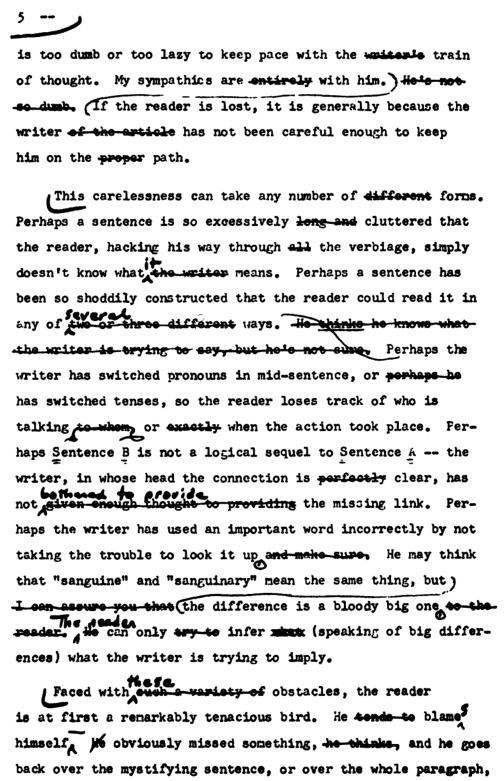
\includegraphics[width=0.9\textwidth]{figure/fig1-1.png}
\end{figure}


\begin{figure}[!htb]
\centering
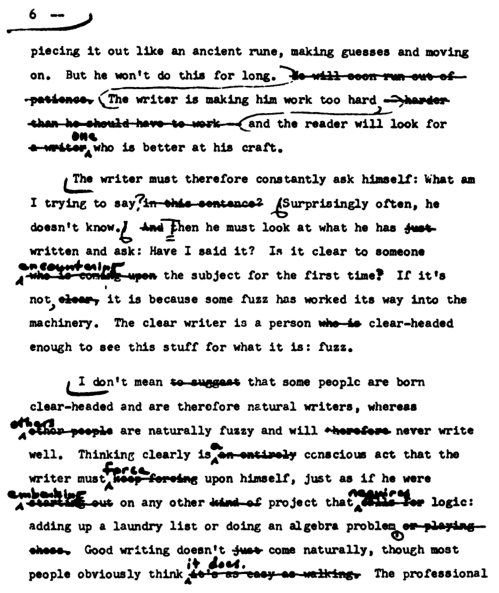
\includegraphics[width=0.9\textwidth]{figure/fig1-2.png}
\end{figure}


以上是《写作法宝》第一版本章终稿的两页。虽然这两页看起来像第一稿,其实已经修改和重新打过四五遍了——几乎每隔一页都是如此。每次修改我都尽力使所写的文字更紧凑、有力、精确,剔除所有无用的部分。然后再过一遍,朗读一遍,每次都惊讶地发现仍有许多赘词可以去除。(在后几版中,我去除了用来表示“作者”与“读者”的性别歧视性代词“他”。)
\chapter{激励工具}
上一章我们批驳了一系列“貌似有理”的不写作的理由,传递的信息是清楚的:根据计划来安排写作。计划表造就了高效的写作者,这是他们为什么能写出那么多作品的原因。不过有可能你在计划的写作时间里无所事事:你坐下来,泡上咖啡,打开电脑,却不知道要写点什么。改过自新的突击写作者通常都不懂如何管理他们的写作时间。因为他们以往的激励工具是“最后期限”和“罪恶感”,他们没有规划目标、同时管理多个写作任务和执行计划的经验。本章将介绍一些常见的能够提升你的写作动机和提高写作成效的激励工具。这些工具起作用的前提是你已经在按照计划表行事。如果你还没有这样做,那你尽可以固执地继续你临时突击的节奏。

\section{制定目标}
和商人一样,学者也喜欢讨论目标。有些学者非常痴迷于目标、举措和战略计划,所以他们成了院长或教务长。目标值得我们好好关注。清晰的目标本身就是直接的激励——它们能够帮助人们制订计划,采取有效行动并因为目标达成而感到自豪(Bandura, 1997)。没有清晰的计划,人们的行动是散漫而毫无方向的(Lewin, 1935)。为了能够写得更多,你需要明确写作目标。这个并不像听上去那样容易,计划常常因为目标设定不当而跑偏方向。设定正确的目标可帮助你成为一个高效的写作者。

那么你该怎样设定目标呢?首先要意识到目标设定是写作过程的一个环节。花上一个写作时间段来好好理清你的写作目标是个不错的主意,我通常一个月整理一次。计划是写作的一部分,所以计划多的人写得也多。第二步是把你的目标逐条列出来——这些目标是具体的需要完成的写作任务。例如修改和重新提交论文,开始写一篇新的文章,接受邀请为某一本合集写一个章节,把你去年写了一半的那篇论文重新捡起来,写一篇课题经费申请报告,或是写一本书。

你想写些什么?当悔过的突击写作者首次设定目标时,通常只有一个任务——是过去三个月以来他们心头一直在回避的那个恐怖的任务。当然要把这个列出来,但是不能仅此而已。在未来的几个月里,你还有什么其他想写的呢?是否在看得见的将来就有一个课题申请要截止了?在你的文件柜里是否有一个还没有发表的实验数据值得你再好好琢磨一下?是否有一篇一直想写而未写的评论文章?把这本书暂时放下,找些纸来,天马行空地列一些你想写的东西。

你决定了要写些什么以后——也许这张单子看起来很长——现在你需要把这些目标写下来。在你的写作过程中不断更新这份东西是浪费时间,所以找一块白板或者公告板,放在你的写字台旁边,然后骄傲地把你的目标一一列在上面。一个突击写作者在这么长的计划面前会感到非常焦虑,但是你有时间表啊!你会自问 “我能完成吗?”自律性强的写作者会大致想一想要花几个星期来完成单子上列的这些内容。在这个单子上划去一项任务是非常令人开心的。你可以贴个笑脸在上面,如果这是你的风格的话。

第三步是把每天要写的目标尽可能具体化。当你真的坐下来为了你的目标奋斗的时候,你需要把这些目标变成一个个小的目标。 “修改这篇论文”是一个写作任务,但是对于决定要写些什么而言,这个表述过于宽泛了。每当你开始工作的时候,都需要花一点时间想一下当天你想完成些什么。“写论文”这样的目标太宽泛了,你需要具体的目标。这里列举一些具体目标的范例:
\begin{itemize}
  \item 至少写200个字;
  \item 把昨天写的草稿打印出来,阅读和修改;
  \item 制订新的写作目标并把它们写在白板上;
  \item 把总论部分的前三段写好;
  \item 补充所有参考文献,然后把引文和参考文献梳理清楚;
  \item 重读津泽(Zinsser, 2001)的书的第二十二章和第二十四章,给自己充充电;
  \item 继续把昨天的“设定目标”部分写完;
  \item 头脑风暴,然后把新论文的大纲写好;
  \item 重读评审人的评论并把要修改的部分一一列出;
  \item 校对清样并寄出。
\end{itemize}

有些人对在目标里列出字数和段落数感到很吃惊。记住,这些是具体的目标。要着手完成一个宽泛的目如——如“修改和重新提交这篇论文”——是很难的,但是要理解“至少写200个字”很容易——你坐下来,打字。精力旺盛的安东尼·特罗洛普(Anthony Trollope)写作的时候会戴一块手表,他的具体目标是15分钟写250个字(Trollope, 1883/1999)。一定要养成制订具体、集中、详细的写作目标的习惯,这样能够避免不知道做什么和不知道怎么做。


\section{挑选优先项}
现在,你手里有一张写作任务的清单了 。在所有这些任务里,你应该先做什么呢?我问了身边的写作高手们是怎样挑选优先项的。下面是综合我自己和身边高手的经验后给出的一些参考意见。你可以以此为参考,并挑选自己的优先项,把它们写在你的写作任务清单旁边。

{\kaishu 1.校对清样和复审论文}

这一项几乎是所有人的首选。道理很简单,校对清样是论文发表前的最后一步了,而且与其他很多学术写作任务不同,这一项通常有严格的时间节点。出版商们往往需要你快速地校对和复审,通常在48小时内完成。在经历了数月或数年的数据收集和写作过程之后.你为什么还会拖延自己的论文发表呢?快快完成吧。

{\kaishu 2.完成有截止期限的任务}

大多数的写作任务都没有截止期限,所以那些有截止期限的任务都应该在计划表中占有优先位置。有截止期限的任务可能包括受邀写作的部分章节、课题申请报告或是行政报告。有些期限很死——大多数的经费提供机构都过期不候,而有一些期限则比较灵活。就我个人而言,我并不把这一项列为我的优先选项,原因是我已经不像过去那样死抠截止期限了。如果你很好地执行了写作计划,那么你总是能够提前完成。截止期限对突击写作者来说是最大的激励,对于一个严格自律、有良好计划的写作者来说则没有什么用。

{\kaishu 3.修改论文以重新提交}

大多数的论文都会被拒。如果你有幸收到修改并重新提交的通知,千万别浪费了。重新修改后的论文比新提交的论文发表的几率高,所以你应把这一项列为优先项。

{\kaishu 4.评审稿件或课题申请报告}

这一项颇受争议。我的同事们就审稿是否应该被列为优先项有不同的意见。有些人认为这一项属于优先“非写作”项,应该快速完成,但不是用写作时间去完成。有些人对评审论文不怎么感冒,常常放在一边。不过我个人觉得这是一项颇为重要的工作,把它放在比较重要的位置。同行评审的过程与评审人关系甚大。心理学界的审稿流程之慢,已经影响到这个领域的发展。如果每个人都看得快一些,那么每个人也会写得欢快一些。快速地完成评论也有助于和编辑们建立良好的关系,因为他们总是对速度过慢的审稿人意见颇多。对于课题申请报告也是一样:课题评审对申请者而言事关重大,所以还是早点把它们做完为好。

{\kaishu 5.开始写作新的论文}

每一篇发表的论文都是从一份草稿起步的。从头写一篇新的论文对于突击写作者来说很难:他们常常花了几个月才开头,他们也是心血来潮时才做文献综述和数据分析部分的。其实,如果你能照着计划来,写一篇新的文章是相对容易的(与撰写课题申请报告、著作和修改论文相比)。第六章将就实证研究型论文写作给出一些建议。

{\kaishu 6.写各种杂文}

对所有不太重要但是仍然需要完成的写作任务,我们姑且称之为杂文。例如写一篇通讯短文。这能够帮助你暂时从那些主要的写作任务中解脱出来,捣鼓捣鼓些小玩意,获得片刻的安宁和乐趣。

几乎所有我调查的对象都提到,他们会把有研究生参与的写作任务放在特别优先的位置。比如,他们通常会花时间修改一篇要重新提交的论文,但是,如果要写一篇新论文,而这篇论文是与某个研究生合著的,他们会把它放在更为优先的位置。这是明智的建议。我也常常把优先权给那些我不参与实际写作的合著论文。试想一下,你辛辛苦苦地写了草稿,发给第二和第三作者征求修改意见,但是从来得不到反馈,这会是什么感觉?被合著者拖累是令人抓狂的,尤其是当这个合著者还不负责具体写作的时候。突击写作不是一个好习惯,而与人合著时还拖延则更加糟糕。

研究生应该和教授们有着不同的写作优先项。以下清单是我在采访了一些优秀研究生或是刚刚毕业的学生后整理的。

{\kaishu 1.有截止期限的写作任务}

研究生学习期间会有很多有截止期限的写作任务,例如某门课程的作业。很多学生抱怨他们的课程作业占用了太多写作时间,使得他们无法花更多的时间完成更为重要的写作任务,例如硕士论文。这是事实,但是截止期限就是截止期限,而这些小的作业或论文对未来的学术生涯未尝不是一种有益的尝试。如果你需要更多的时间写作,那只能在你的写作计划表里安排更长的时间。经费申请报告——例如研究生奖学金的申请——也同样有截止期限,而且它们非常重要,应该努力尽快完成。

{\kaishu 2.与学位授予相关的写作任务}

研究生学习期间,你需要写很多与学位授予相关的文章,例如硕士学位论文、综合考核报告、资格论文和博士学位论文。这些要想毕业就必须完成的东西最好快点写完。上述这些任务的成果有时候还能转化为可发表的论文,所以很多学生都会把与学位授予相关的论文与真正的专业写作结合起来。

{\kaishu 3.公开发表的专业论文}

科学研究只有在它公开发表,使之得以为同行所阅读和评论之后才能实现其真正的价值。你完成了论文,院系委员会也觉得你干得不错,但这是不够的,只有论文公开发表后学术界的其他同仁才能有机会更仔细地研究你的论文并认识它的价值。优秀的硕士学位论文或博士学位论文应该寄给专业的期刊。此外,你还应该力求在硕士学位论文和博士学位论文以外发表更多的专业论文。你要抓住每一个机会参与研究和专业写作。如果你很好地对写作加以规划,你将是你们项目里最高产的研究生。

{\kaishu 4.其他}

研究生常常写许多五花八门的文章,比如书评或报刊杂文。和其他类型的写作一样,写这一类的文章也是很好的锻炼,也很有意义。不过与专业水准的、存档留案的论文(比如期刊论文或专著的某个章节)比起来,这些杂文就显得不那么重要了。如果要在两个中间作出选择,那就应该把专业写作放在前面。

当我们在讨论选择优先项的时候,总有人会问:“那万一我觉得没什么可写呢?”对教授们来说,极少会感到没东西可写。恰恰相反,大多数我认识的教授都有堆积如山的未发表的数据。收集数据的过程是简单的,写作是困难的。如果你有一些十年前就已完成的实验却从未发表过,那我肯定你需要一段时间才会感到没有东西可写。更何况,写作促进写作。正如博伊斯(Boice, 1990)所发现的,那些定期写作的人会比那些只在灵感来临时写作的人有更多的创见(参见第二章)如果你觉得没有东西可写,那还是花一段写作时间来重新列一下你的写作目标吧。

然而,研究生们或许的确会觉得没有一个现在要跟进的写作任务。也许你刚刚完成了你的论文,暂时没有其他任务;也许你刚刚入学不久。别害怕,这个时候你有两个选择。首先,你可以参与一项正在进行的写作任务。你的导师,跟其他大多数的教授一样,或许正在为一大堆写作任务而头疼。敲开他/她的办公室然后说:“我最近看了一些关于如何成为更好的写作者的书,其中一本建议我敲开您的办公室,然后问问我是否能参与到一些写作任务中来。如果您有一些论文要写或是有一些数据要整理,我愿意帮忙。”很有可能你的导师会大倒苦水。教授们都希望自己的研究生在专业研究和写作方面倍加勤奋,所以你的导师一定会为你想加入而感到高兴。

另一个解决没有东西可写的办法是,你可以用写作时间来做些对专业发展有益的事。我读研究生时得到的最好的建议就是,“总是让自己不断思考”。研究生院是疯狂的,当你在为一大堆截止期限埋头奋斗的时候,你往往会忘了自己的长期目标。每周给自己留些固定时间,就能够利用它们来读些关于写作和教学的书,回顾自己的研究,想想你的职业规划。


\section{监控进展}
大多数人都不清楚自己究竟写了多少东西,是多是少。因为他们总是带着某种沾沾自喜、自我安慰的态度来审视自己,大多数人都认为自己比实际上要来得高效。为了写得更多,你必须带着某种冷峻、客观的态度来监控你的写作进展。有关自我管理的研究表明,仅仅设定目标和选定优先项是不够的:人们必须就达到目标的进程进行监控(Carver \& Scheier, 1998; Duval \& Silvia, 2001)。

监控写作进展有很多激励作用。首先,时时直面你的目标能够加深印象,防止你淡忘。许多人对如何管理他们写的东西很不在行。监控进展能够帮助你关注你正在进行的任务。其次,监控本身也足以帮助你坐下来开始写作。行为研究表明,自我观察本身就能够促进期待行为的发生(Korotitsch \& Nelson-Gray, 1999)。例如,想要存钱的人应该记录他们每天的花销,因为记录他们每天花了多少钱能够让他们节省开支。同理,想要定期写作的人应该追踪他们是否定期坐下来写作了:你放弃了某段写作时间,所以不得不在一个Excel表格里打上一个大大的“零”的时候,你会很奇怪地感到某种鞭策。最后,监控你的写作能够帮助你制订更合理的目标。经过一段时间,你将能积累足够的资料来合理地判断你大概需要多久来完成某项写作任务。制订更合理的目标,反过来又能够保障更高效的写作。

高产的写作者通常都会做这样或那样的监控。方法有很多种。在这部分里,我想介绍一下我的方法。每次我向别人介绍我的方法的时候,他们都给我一个诧异的表情,就好像听说我要拿伯尔尼山犬的毛来做被子似的。我用的系统看起来又蠢笨又牵强,还有点奇怪,不过它的确能帮助我集中精力。我有一个文件名是“写作进程.sav”的SPSS文件,图3.1是它的截图。我记录月份、日期、星期和年份。这些变量帮助我定位某一个日期。统计项是字数、目标和任务。在字数一栏,我键入每天我写的字数。字数统计工具能够轻松地告诉我文章的字数;每天开始和结束写作的时候都统计一下就能清晰地显示出一天的成果。你会注意到字数这一栏有很多空白。我之前已经强调过了,写作包含很多任务,不仅仅是码字。有时候我读些论文,有时候我填写课题申请表,有时候我重读需要修改并重新提交的论文。这些日子的字数一栏就会是空白的。设置目标一栏的目的就是回顾我是否完成了当天的目标。我个人的目标很简单,坐下来做些有利于推进研究的事,所以我会把这个变量记为\{0=未完成,1=完成\}。图3.1所示的那段时间我干得不错;只有7月5日那天我未完成我的既定目标,其他日子我都完成了。任务一栏用来描述我当天的任务。如实记录任务能够让你更清楚地知道你要花多少时间来完成一项任务。有时候会觉得某个任务没完没了,但是有可能它比你记忆中的已经简化了而你没有发觉。

\begin{figure}[!htb]
\label{fig3-1}
\centering
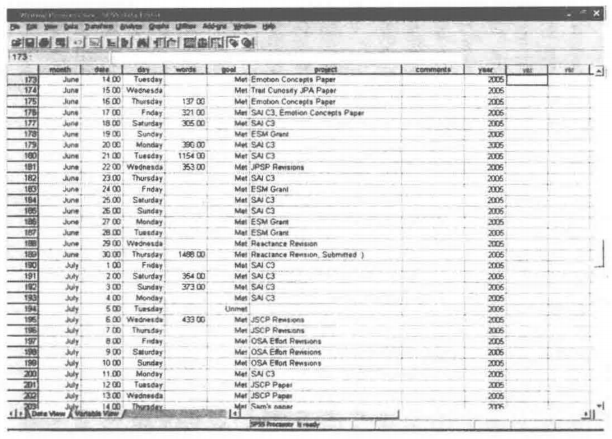
\includegraphics[width=0.9\textwidth]{fig3-1.png}
\caption{我用“写作进程.sav”文件来监控自己的写作进程}
\end{figure}

那些还死抱着各种无力借口的突击写作者可能会说“但是我不会用SPSS”或者“可是我只用SAS”!其实任何统计软件或者制表软件都可以做这件事,实在不行,画好线的笔记本和铅笔总是有的。监控本身才是关键,技术问题不是问题。不过,统计软件能够让你深入挖掘你的写作数据。如果你是一个统计控——这年头又有谁不是呢——那么你会爱上获得你的写作数据的感觉。我写了一个简单的SPSS公式来计算一些可见的数据和柱状图。当我开始写一篇新的文章时,我平均每天写789个字,如图3.2所示。听起来不是很多,不过字数逐日增加。图3.3显示的是每个月的目标完成情况。根据数据,在过去的12个月里,我在计划写作的日子中有97\%的日子实际坐下来写作了。我不是完美的,不过我对这个数据还是满意的。监控是为了改进,如果有一天这个数据达到100\%,我会感到非常骄傲。如果你很好奇,你还可以把目标达成情况和字数都按照天数来统计。所以,如果有人问我能写多少,我会回答97\%的工作日我都在写作,且每天我平均写789个字。他们可能会给我一个“伯尔尼山犬毛被子”的面孔,但这无所谓。

\begin{figure}[!htb]
\label{fig3-2}
\centering
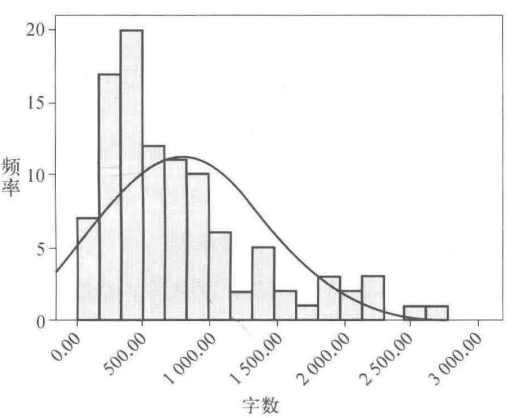
\includegraphics[width=0.9\textwidth]{fig3-2.png}
\caption{过去12个月每天的平均写作字数}
\end{figure}


\begin{figure}[!htb]
\label{fig3-3}
\centering
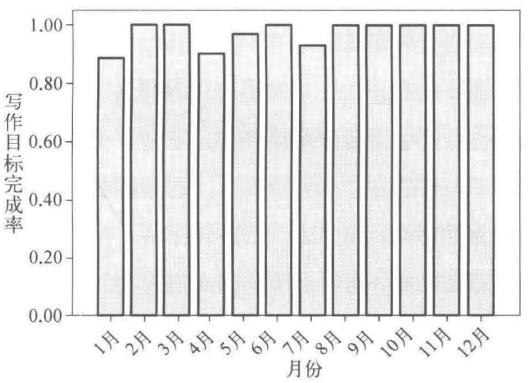
\includegraphics[width=0.9\textwidth]{fig3-3.png}
\caption{过去12个月每月的写作目标完成率}
\end{figure}


当你完成一项写作任务时,别忘了奖励自己。自我强化和依随性管理被证实对培养好习惯有很大的帮助(Skinner, 1987)。当你提交了一篇论文或是一份课题经费申请报告,给自己买杯好咖啡或是吃一顿奢侈的午餐,或者买一张古老的好莱坞-维克菲尔德式的书桌。写作的回报往往是滞后的——通常都要等上好几个月才能有杂志编辑或者经费评审委员会的消息——所以即时的自我奖励能够帮助你维持兴趣。不过,只有傻瓜才会以偷懒不写作的方式来奖励自己。永远不要以不写作的方式作为对写得好的奖励,以抛弃你的写作时间作为奖励,就好比以抽一支烟来奖励你戒烟成功。写作计划的有效执行有赖于超强的习惯掌控力:不要丢掉好的写作习惯。


\section{文思枯竭}
“等一下,”你也许会说,“到目前为止,这本书还没有提到任何关于文思枯竭的问题。当然啦,你可以制订计划,设定目标,然后监控进展,然而如果你实在写不出来怎么办?”我非常喜欢“文思枯竭”,这与我喜欢树精或是会说话的林中动物的道理是一样的——它们都很令人着迷,而且它们都不存在。当人们跟我说他们有时候真的会文思枯竭,我总是问他们,“你们到底要写什么?”学术写作者是不可能文思枯竭的。千万不要把自己和那些在艺术系教创作的朋友混为一谈。你又不是在创作一个长篇故事或是在写一个直指内心深处某个神秘角落的深刻隐喻。你对方差的精妙分析不会让读者们感动落泪,倒是有可能枯燥得让人掉眼泪。人们也不会影印你的参考文献目录并发给朋友们,期待能够给他们带去灵感与启迪。小说家和诗人是充满诗情画意的风景画家和肖像画家;学术写作者则是手握大型喷漆器重新粉刷地下室的油漆工。

文思枯竭是一个典型的倾向性谬论:对行为的描述同时被用来解释被描述的行为本身。所谓文思枯竭,说白了就是什么都没写。你说自己文思枯竭了,所以写不出东西,就相当于你说自己写不出东西是因为你什么都没写。这样的说法毫无意义可言。治疗文思枯竭的办法——如果你可以治愈无病呻吟——就是写作本身。建议重读第二章博伊斯(Boice, 1990)的实验。那个研究表明,苦苦挣扎的写作者们只要按照计划不断写作,就能写出很多东西——就这么简单。相反,那些非要等待“灵感”的人几乎什么也写不出。如果你真的文思枯竭,你有三个选择:(1)放下你手上正在摆弄的诗集,重新回到你的期刊论文写作中;(2)说服树精或会说话的动物们帮你写问题讨论部分;(3)重新制订你的写作计划,然后重新执行它。

就好像外星人只绑架相信存在外星人绑架事件的人一样,文思枯竭只会发生在相信有文思枯竭这回事的人身上。写作计划——这是个很神奇的东西——最神秘的部分就是,有计划的作者不会感到文思枯竭,不管到底有没有这回事。高效的写作者无论想不想写,都会按时写作。有时候他们写得不多——写作是件艰难的事情,但是不管怎样,他们都会坐下来写,不为那些虚无缥缈的事情所干扰。

\section{小结}
本章介绍了一些能够帮助你成为一个更高产的写作者的激励措施。制订好写作计划表以后,你需要确定写作目标并把它们写下来。然后,在你坐下来写作以前,先花一分钟想一想你今天想干什么。选定优先项能够马上帮助你摆脱同时进行多个写作任务的压力。监控你的写作能够让你集中精力完成目标,监督你不要放弃任何一天,告诉你你能写得多好,还能提供足够的数据让那些怀疑你的突击写作者闭嘴。任何能把本章提到的建议都一一做到的人,毫无疑问都能写得很多。
\chapter{风格}
作者努力写出简洁的句子,但总有那肿胀的怪物埋伏在暗处捣乱。有关写作初期的告诫就谈到此。

“但是,”你也许会说,“如果我去除你认为是赘语的所有部分,如果我将每一句话都剥到只剩骨头,那我还能剩下什么?”这个问题问得合理。简洁推到极致也可能会指向一种不比“狄克喜欢珍妮”和“看斯波特跑”这样的句子更复杂多少的风格。

我将首先从木匠手艺的层面回答这个问题。然后涉及更大的问题,即作者是谁,如何保护作者的身份。

很少有人意识到自己写得多么糟糕。没人向他们指出有多少过剩或含糊的词语溜进自己的写作风格中,以及它们如何阻碍了作者想说的话。假如你给我一篇八页的文章,我叫你删减到四页,你会叫喊说那做不到。然后你回家去做,结果会好得多。之后便是难的部分:删减到三页。

要点是你必须先将自己的写作拆开,然后再搭建起来。你必须知道基本工具是什么,以及其预设的作用是什么。再拿那个木匠手艺比喻为列,首先必须锯好木头,然后钉钉子。之后,你如果有雅兴,再切修棱角、添加别致的顶部。但千万不要忘记你是在练习一项基于一定原则之下的技能。如果钉子不牢,房子就会坍塌。如果动词不牢、句子结构摇晃,句子就会分崩离析。

我得承认,有一些非虚构作家,如汤姆·沃尔夫和诺曼·梅勒,他们建构起了不起的房屋。但这些作家花了许多年来学习技艺,最终才搭建起神奇的塔楼和空中花园,使我们这些从未梦想过如此装饰的人惊叹不已。他们知道自己在做什么。没人一夜间就成为汤姆·沃尔夫,就连他本人也不能。

那么首先要学会钉钉子。如果你所建房屋既结实又好用,就该对具简洁之力感到满意。

但你没有耐心去成就一种“风格”——去修饰简朴的词语,这样读者就会把你认作一种特殊的人。你只会寻觅花哨的比喻、华而不实的形容词,就好像“风格”是什么能在风格店买到的东西,是可以用装饰漆那鲜亮的颜色装饰词语的东西。(装饰漆是装修工用的彩色漆。)风格店并不存在,风格对于写作中的人是有机体,就像头发是他自己身体的一部分,或者假如他秃顶,那么就是他身体缺乏的那部分。试图添加风格就像加假发在秃头上。瞧第一眼时,之前秃顶的人看起来年轻,甚至还帅气,但瞧第二眼时——看假发时人们总会瞧第二眼——那人看起来就不对劲了。这里的问题并非是他看起来没有梳理好,他梳理得很好,我们真得敬佩假发匠人的高超工艺,问题是他看起来不像自己了。

这个问题是那些特意装点自己文体的作家的通病。你丧失的是使你自己独一无二之处。读者会看出你是否在装腔作势。读者要的是,与他们交谈之人听起来是真挚的。因此,写作的一个基本准则是:做你自己。

然而,没有什么准则比这一条更难遵循。这要求作者做到两件事,而按其新陈代谢的本能来说,这些都是难以做到的。他们必须放松,必须有信心。

叫作者放松就像在检查疝气时叫人放松一样;至于信心,看,他多么僵硬地坐着,眼睛直勾勾地盯着等待他造词儿的电脑屏幕。看,他多么频繁地站起来找吃的或喝的。作者会想方设法躲避写作实践。我可以证明我在报社工作期间,作为记者,我每小时去饮水机的次数大大超过身体对水的需求。

如何拯救作者出苦海呢?很不幸,并没有拯救的办法。我只能安慰大家说并非只有你的遭遇如此。有些日子好过一些,另一些日子则难熬到让你绝望,不再想写作。大家都有过这些日子,而且还会有更多这样的日子。

当然,最好还是尽量减少难熬的日子。这就使我回到如何放松这个问题上来。

假如你就是那位坐下来准备写作的作者。你想到你写的文章必须具有一定的长度,不然就不会显得重要。你想到文章印出来有多么庄严。你想到那么多人阅读你的文章。你想到文章必须具有重重的权威性。你想到文章的风格必须炫目。怪不得你会浑身发紧:你在忙于想着自己甚至还未开始的文章写完之后所要承担的巨大责任。而你发誓要对这一任务称职,于是四处找大词,找那些如果你不是想刻意给人突出印象就根本想不到的词,并且一头栽进去。

第一段是一场灾难——整段话成了似乎来自机器的一系列笼统词语的组合。人是不会那样写的。第二段也好不了多少。但是第三段开始有点儿人情味,而到了第四段你开始听起来像自己了。你开始放松了。令人称奇的是,编辑会常常删掉文章的前三四段,甚至前几页,而始于作者听起来开始像自己的部分。前几段的问题不只是缺乏人情味和浮夸华丽,而是根本就没说什么,只是刻意地要写出一个花哨的前言。作为编辑,我总是在寻找说类似以下这样话的句子:“我永远不会忘记那一天……”这时我就想,“啊哈!真人说话啦!”

作者用第一人称写作显然是最自然的。写作是把两个人之间密切的交往付诸笔端,写作保持人情味才会顺畅。因此我敦促人们用第一人称写作,用“我”或“我们”。但大家表示抗拒。

“说我认为什么,或者我感觉什么,那个我是谁啊?”他们问。

“不说你认为什么,那么你又是谁呢?”我回答他们,“只有一个你。没有任何其他人想的和感觉的一模一样。”

“可是没人会在乎我的观点,”他们说,“那样会让我觉得太突出了。”

“如果你对他们讲述有趣的事,他们会在乎的,”我说,“而且要用自然而然的词语讲述。”

然而,要作者用“我”并不容易。他们认为必须先赢得袒露自己情感和思想的权利,不然就会显得自以为是,或者不庄重。此类恐惧也影响了学术界,因而出现了学术性的“某人/有人”的用法(“有人不能苟同于莫尔特比博士对于人类状况的观点”),或者无人称的用法(“希望费尔特教授的专著会理所当然地拥有更广泛的读者”)。我可不想见用“有人/某人”这样的人——很乏味。我要的是对自己的话题有激情的教授来向我诉说该话题为何使他着迷。

我意识到写作中有广大领域不允许用“我”。报纸不要第一人称代词“我”用于新闻报道中;许多杂志也不要它出现在文章中;商业、社会机构不要它用在大量发送到美国家庭的报告中;大学不让把“我”用在学期论文或学位论文中;还有英语教师也不赞成用第一人称代词,除非是作为书面语的“我们”(“我们在麦尔维尔对于白鲸的象征用法中看到……”)。以上那些禁用是合理的。报纸文章就应该由客观报道的新闻构成。在学生没经过一番挣扎学会从其内在优点和外在评论评价一部作品之前,教师不希望学生避重就轻地发表意见——“我觉得哈姆雷特挺愚蠢”。我也理解教师的这些想法。“我”这个词有可能变成某种自我陶醉和自我逃避的工具。

然而,我们的社会已经变得害怕袒露自己的心声。向我们发送宣传品、寻求支持的社会机构听起来惊人地相似,但所有这些机构——医院、学校、图书馆、博物馆、动物园等——当然是由那些有不同梦想和展望的男男女女创建和管理的。这些人都在哪儿?在所有那些非人称的被动语态句子中,如“已经采取行动”和“重点已经确定”,很难瞧见他们的真面目。

即使是在不允许用“我”的时候,也有可能传达一种个性化的我的意思。政治专栏作家詹姆斯·赖斯顿在专栏写作中并没用“我”,但我却很清楚他是什么样的人,对其他很多随笔作家和记者,我也可以这么说。好作家在字里行间是看得见的。如果不允许你用“我”,写作时至少要用“我”思考,或者第一稿用第一人称写,然后再把“我”去掉。这样能预热你的非人称风格。

风格与心理绑在一起,写作的心理机制根深蒂固。我们表达自己的特有方式,或由于“作者心理阻滞”而没能表达好自己的原因,部分埋藏于潜意识心理中。作者心理阻滞的种类就像作家种类一样多,我也没有捋清它们的意图。这是一本薄书,我的名字也不叫西格蒙德·弗洛伊德。

但是我也注意到避免“我”的新理由:美国人在言辞上不愿意冒任何风险。我们的上一辈领袖们直言不讳自己的立场和信仰,现今的领袖们却千方百计地巧用词语逃避这一宿命。看看他们如何在电视采访中拐弯抹角,就是不立场鲜明。我记得有一次福特总统向一行来访的商人保证他的财政政策会奏效。他说:“每月我们所看见的是不断增亮的云彩,此外别无他物。”我对此的理解是那云彩还相当黑。福特的句子含义模糊不清,等于什么也没说,却给他的选民打了镇静剂。

后来的当局者们也并没有起色。国防部长卡斯帕·温伯格在1984年评价波兰危机时说:“有继续严重关注的余地,而且形势仍然严重。严重的形势持续越长,严重关注的余地也就越多。”老布什总统被问及他有关突击步枪问题的立场时说:“有不同的群体认为可以禁止某种枪支。我不在其列。我是在那些深刻关注者之列。”

不过我的全能冠军当属70年代身为四任主要内阁成员的艾略特·理查森。很难确定从他那模棱两可的句子宝库中选哪一句,还是看这句吧:“但是呢,均衡地来讲,我认为少数族裔及妇女维权行动还是取得了一定的成果。”\footnote{原文如下: And yet, on balance, affirmative action has, I think, been a qualified success.}一句13个单词的话中就有5个词含义模糊。在现代公共话语中,我给它最空泛句子一等奖,但与其媲美的还有他分析如何消除生产线工人单调乏味的句子: “这样呢,最后,我形成一个坚定的信念,我在开始提到过:就是这个问题太新,无法最终判断。”


那就是坚定的信念吗?像摇摇晃晃来回摆动的年迈拳击手这样的领袖不能鼓舞信心——也不配鼓舞信心。作家也是如此。推销你自己,你的题材就会发挥自己的吸引力。相信自我身份,相信自己的见解。写作是一种自我行为,你得承认这一点。要全力以赴使自己不断向前。
\chapter{简洁、单刀直入的文风}
学术期刊散发着垃圾写作的酸腐味——我总是把期刊放在离书桌最远的书架上,以免被熏到。但是如果你有机会与这些文章的作者面对面交流,你会发现他们对自己的研究津津乐道,他们的口头表达是那样清晰、生动和有趣。哪里出了问题?尽管这本书的主题是写得更多,而不是写得更好,但你还是应该花点时间来掌握一些要领,让你的作品更有力度。如果人们坚持执行写作计划,大概一个星期以后他们就能写得更多,要写得更好则需要更长的时间来学习——所以我们应该从现在就开始。本章将介绍几个能够帮助你提高写作水平的小技巧。

\section{诊断问题}
有三个原因会导致写作水平偏低。首先,学者们喜欢显摆聪明。有一则德国格言说:“水面颜色深的湖必是深湖”所以,学者们常常弃好词而不用。比如,他们不用“聪明的”(smart),却用“老练的”(sophisticated)或“渊博的”(erudite)。我应该这样说,“水体的透明度的最小值往往与水的深度之间有着极高的相关性(p<0.05)”。其次,学者们从未学过好好写作。他们在研究生院的导师可能不是一个好榜样,而他们引以为榜样的期刊文章也散发着酸腐的垃圾味。最后,大多数学者都没有花足够的时间来成为一名优秀的写作者。和其他所有的技能一样,写作技能也需要长时间的勤学苦练(Ericsson, Krampe \& Tesch-Romer, 1993)。人们必须学习好的写作规则,然后花大量的时间来练习。

为了解决第一个问题,你必须修正对学术写作的态度。也许有些读者会因为你写的东西晦涩难懂而觉得你很聪明,但是你并不需要这样毫无眼光的读者。大多数的科学家都会被好的观点和有趣的发现吸引,所以不要把你的意见藏在一大堆垃圾英语背后。为了解决第二个问题,仔细地阅读这一章,然后买一些其他关于写作的书来读。本书“推荐阅读:那些关于写作的好书”部分附有关于文风和语法的参考书目,或许对你有所帮助。为了解决第三个问题,你需要阅读上述书籍,并在写作时多加练习。要不了多久,你就会逐渐形成独具一格的文字风格,而不再是那个让人不知所云的无名氏了。

\section{选择“好词”}
写作的核心在于用好词。为了写得好,你必须选择“好词(good words)”。英语中包含很多词,其中有很多简短、有表现力而且常见的词——要选用这些词。避免用那些听起来很深奥的时髦词组,更不要用那些学术腔太重的词。除了帮你提高写作水平,选择“好词”也是对读者的一种尊重,因为对他们来说,英语可能是他们的第二、第三或者第四语言。外国学者常常在阅读文章的时候备有双语词典,如果你选的词不在词典里,他们就理解不了。他们会怪自己误解了你的意思,其实你才是应该被责备的人,因为你没有顾及他们的实际情况。

“那专业词汇呢?”你也许会问,“我怎么可以不用‘刺激呈现的异步性(stimulus onset asynchrony)’来写一篇关于刺激呈现的异步性的文章?”科学在需要的时候会创造出新的词——这些专业词汇是有用的。如果用常用的词来解释,这些专业词汇是很容易被理解的。我们应该保留科学词汇,剔除那些从商学、市场学、政治学和军事学那里借用来的词汇。我们不需要诸如“物质激励(incentivize)”或“瞄准(target)”之类的动词,也只有玻璃清洗工才需要“透明(transparent)”之类的形容词。为了连贯,请重复使用同样的专业词汇。不断变换的心理学专业概念会把你的读者搞晕:

{\kaishu 前:神经过敏症指标高的人比体验厌恶情感状态倾向指标低的人反应慢。

Before: People high in neuroticism responded slower than people low in the tendency to experience aversive affective states.

后:神经过敏症指标高的人比神经过敏症指标低的人反应慢。

After: People high in neuroticism responded slower than people low in neuroticism.}

而且有些专业词汇真的是糟糕透顶,所以不要不假思索地引用你在专业期刊上看到的词汇。发展心理学家对“道(path)”和“路(way)”都不满意,他们喜欢用“路径(pathway)”;在某些吹嘘的场合,“路径”变成了“轨道(trajectories)”。认知心理学家喜欢“澄清(clarify)”什么是“消除歧义(disambiguate)”。临床心理学家喜欢说病人“呈现(present)”出某种症状,感觉对方好像是一个情绪低落的管家,托着一个盛满“负面情绪”或“低质量睡眠”的大盘子。临床医生也不再用“医嘱(manual)”和“遵医嘱(follow manual)”,他们发明了“医疗干预(manualized interventions)”一词。情感心理学家生怕他们的读者不理解“评价(appraisal)”这个词的意义,他们喜欢说“认知评价(cognitive appraisal)”“主体评价(subjective appraisal)”有些人还是怕别人不理解,索性说“主体认知评价(subjective cognitive appraisal)”。做跨学科研究的心理学家提出了“生物——社会”模型(biosocial models)、“社会——心理”模型(psychosocial models),最近又有了“生物——心理——社会精神”模型(biopsychosocialspiritual models),用以取代原有的狭隘的“生物——心理——社会”模型(biopsychosocial models)。

心理学家特别青眯“坏词(bad words)”,不过他们不说“坏(bad)”,而是代之以“deficient(有缺点的)”或是“suboptimal(非最理想的)”。心理学家喜欢用“现有文献(existing literature)”, 难道我还需要阅读和引用“不存在的文献(nonexistent literature)”吗?任何在读文献的心理学家都应该知道我们这些专业期刊就是这样“可怕而真实”。“现存文献(extant literature)”是同一宗罪的升级版。那些写某两样东西之间“失联(disconnect)”的心理学家恐怕是与他们的字典“失联”了,因为他们本可以在字典里找到无数更好的词,如“差异(difference)”“区别(distinction)”“分离(seperation)”和“差距(gap)”。有些人在写某一关于某一问题的论文时,把“人”(a person)称为“个体”(individual)而把“人们”(people)称为“个体们”(individuals)。这些人忘记了“个体”是一个模糊的概念:试想,“我们观察一个个体\_\_\_\_ 。”画横线部分应该补充一个名词(例如:兔子)还是一个动词(例如:走路)?你在和朋友说话的时候从不说“个体”或“个体们”,那为什么在和广大的科学界同仁交流的时候要装腔作势地这么说呢?选个对的词,比如人(person)或人们(people)就可以了。而“persons”则更为可恨,这样的词大概只有小镇警长在寻找失踪人口时才会用到吧。

说到“人们(people)”,我在描述我的研究参与者时已经不再用“参与者(participants)”一词了。我的朋友们有研究鸟类、婴儿、老鼠或是学区的,他们的“参与者”和我的完全不同。我研究的是成年人,所以“人(person)”或“人们(people)”是对我的研究对象的准确界定。如果这个决定让你不安,别害怕——美国心理学会(APA)不像时尚界,这里没有“警察”。“参与者”是一个模糊的词,心理学家应该选择更确切的词。比方说,有些研究人员是从儿童、教师和家长那里收集资料来研究儿童心理学的,他们的参与者就应该是上述三个类别的人。不要觉得有什么不妥,就应该称他们为儿童、教师和家长。如果你研究老年人或是年轻人的认知过程,为什么不在你的研究方法和结论部分称他们为老年人或是年轻人?现在就把你的研究方法部分重新写一遍,把所有的“参与者”都改成更为确切的词,这样你会觉得舒服很多。

一些缩略词和首字母简称也是不妥的。我见过有些人把很常见的词,比如“焦虑”(anxiety)或“沮丧”(depression)缩写为ANX和DEP,把简单的词组,比如“引发焦虑”(anxious arousal)和“缺乏快乐感而沮丧”(anhedonic depression)简写成ANXAR和ANDEP, 然后兴奋地讨论ANX、ANDEP、DEP和ANXAR的区别。缩略词和首字母简称只在比它们代表的原词(或词组)更易于理解的情况下才有用。SES(社会经济地位)和ANOVA(方差分析)是好的缩写,ANX和DEP则不是。有些作者认为他们用简称代替常用词能够避免行文冗长。比如写一本关于如何写得更多的书,他们会想着把“写得更多”缩写为WAL。其实读者会觉得读这样的缩写比读原词更乏味。为了避免拐弯抹角,你应该少用缩略词。

删去诸如“非常(very)”“相当(quite)”“基本上(basically)”“实际上(actually)”“事实上(virtually)”“极端地(extremely)”“明显地(remarkably)”“完全地(completely)”“根本(at all)”之类的词。基本上,这些相当无用的词事实上毫无意义,它们事实上就像水草,实际上会完全地阻塞你的句子。在《垃圾英语》一书中,肯·史密斯(Ken Smith, 2001: 98)把这些词称为“寄生强化剂”(parasitic intensifiers)。

{\kaishu 原本含义确切的词现在好像需要附加这些强化剂才能恢复原有的能量。现如今,表达观点或是反对的立场时非要加上“有价值的”或“坚决的”之类的词,否则就会显得不温不火。这些强化剂削弱了原意。}

如果你真心领会了斯特伦克和怀特(Strunk \& White, 2000: 23)关于“省略无用的词”的建议,但是又不太确定哪些是无用的词,那么上述这些“寄生强化剂”基本上就是应该完全删除的。


\section{写出有力度的句子}
现在你对遣词有所体会了——“我上篇文章有没有用‘个体’?”——那么是时候想想如何造句了。“每当你造句的时候,”谢里丹·贝克(Sheridan Baker, 1969: 27)这样写道,“应该就像呼吸一样自然,或许也同样缺少变化”。不断重复类似句型的作者,就好像在不断地使用复读机。英语有三种不同类型的句式:简单句、复合句和复杂句(Baker, 1969; Hale, 1999)。简单句只有一个主——谓结构。学者们对清晰的简单句不屑一顾。这实在可惜。复合句有两个从句,每个句子能够独立存在。有时候用关联词来连接非独立从句,有时候分号能起到同样的作用。与简单句和复合句不同,复杂句包括独立从句和非独立从句。复杂句如果用得好,能够使你的文章干净利落、张弛有度。

在自我感觉良好的时候,我相信并列句是为心理学家发明的。我们总是在写关系、对照和比较:外向型指标高的人和外向型指标低的人、控制组和实验组、时间段一发生的事情和时间段二发生的事情。好的写作者合理地运用并列句来描述关系;拙劣的写作者则尽量不使用并列句,因为他们觉得并列句很啰嗦,相反,他们通过变换词语和句式发明了很多别扭的句子。

{\kaishu 前:双任务组的人在一组“嘟嘟”声的引领下阅读一列词汇清单;另一个组的另外一些参与者仅阅读词汇而不会听到任何声音(“控制组”)。

后:双任务组的人在一组“嘟嘟”声的引领下阅读一列词汇清单;控制组的人仅阅读词汇清单。}

有些并列句式用“标准——变量”的格式:先描述共性,而后解释差异。

{\kaishu 更好:每个人都阅读一列词汇清单,双任务组的人在一组“嘟嘟”声的引领下阅读,而控制组的人仅阅读。

更好:每个人看一组20幅画。控制组的人只是看一看这些画,评估组的人则要标出对每幅画的喜爱程度。}

很多人根本不知道如何用分号——这个符号是并列句的最佳搭档,却常被忽略。就像人们不喜欢球迷或俱乐部的年册一样,很多作者从高中就养成的对分号的不信任绝对是一种偏见。我们要解决这个问题——我们要分号。分号必须连接独立从句;句子的任一部分必须能够独立存在。与句号不同,分号表示两句句子间的紧密关系。与逗号及随之出现的“和”也不同,分号表示两个部分间的平衡。分号是理想的连接两个并列句的工具:

{\kaishu 前:在时间段1, 人们阅读词汇。在时间段2,他们尝试记住尽可能多的词。

后:在时间段1, 人们阅读词汇;在时间段2,他们尝试记住尽可能多的词。

前:阅读组的人阅读词汇,听力组的人听这些词的朗读录音。

后:阅读组的人阅读词汇;听力组的人听这些词的朗读录音。}

除了学会使用分号之外,我们还需要认识一位新朋友——破折号。好的写作者对破折号很上瘾。破折号——严格意义上,它们应被称为“长破折号”——让句子显得干脆。破折号主要有两大用途(Gordon, 2003)。首先,单用一个破折号能够关联一个从句或词组直到句子的最后部分。你在本章已经读到很多这样的例子:

{\kaishu 1.学术期刊散发着垃圾写作的酸腐味——我总是把期刊放在离书桌最远的书架上,以免被熏到。

2.我们要解决这个问题——我们需要分号。

3.除了学会使用分号外,我们还需要认识一个新朋友——破折号。}

其次,用两个破折号能够连接插入语。比如你前面读到的:

{\kaishu 1.现在你对遣词有所体会了——“我上篇文章有没有用‘个体’——那么是时候想想如何造句了。

2.破折号——严格意义上,它们应被称为“长破折号”——让句子显得干脆。}

请你在下次描述参与者和研究设计部分的时候,尝试运用破折号:

{\kaishu 尚可:42个成年人参与了这个实验。其中有12位女士和30位男士。

更好:42个成年人——12位女士和30位男士——参与了这个实验。}

长破折号有一个鲜为人知的兄弟:短破折号。短破折号连接两个概念。这是另一种更简洁的“中间”的表达方式。很少有人能准确地运用短破折号;他们用连字符,且常常带来令人尴尬的后果。发展心理学家对家长—孩子行为感兴趣,但是这并不是说家长们有时候表现得像个孩子——他们用的“家长—孩子”是“家长与孩子间的行为”的缩写。好的写作者知道“教师—家长会议”(短破折号)与“教师-家长会议”(连字符)之间的区别。我们学校的一位研究人员贴了一张有关“婴
儿-家长互动研究”的海报(“先别管少女妈妈了——婴儿妈妈都出来啦!”),现在是时候好好感谢那些默默地为你修改短破折号错误的出版界英雄啦。

你可以尝试用同位语来使句意更为确定。因为句中这些词组表示某种关系,所以你能够省略那些用来连接句子各个部分的连接词。

{\kaishu 前:反事实思维,被定义为关于并未发生过的事情的思维,表现了认知与情感间的交叉。

后:反事实思维,即关于并未发生过的事情的思维,表现了认知与情感间的交叉。

更好:反事实思维——关于并未发生过的事情的思维——表现了认知与情感间的交叉。

前:面部表情研究是认知与情感研究领域的一个热门话题,通过对其研究解决了情感结构上由来已久的矛盾。

后:面部表情研究,认知与情感研究领域的热门话题,解决了情感结构上由来已久的矛盾。}

最后,你能够通过检查学术写作中的两个通病来辨识哪些句子是弱句子。第一个通病,“这样(such that)”病毒。它折磨着那些惧怕简单句的作者。为了避免出现简单句,他们用“这样”来连接一个松松垮垮的主句和他们真正想写的从句。再也不要用“这样”了。用Word自带的“查找”功能把你的文章里所有的“这样”都找出来。如果你找到了,有三种处理办法:把“这样”之前的部分删除,用冒号或破折号替换“这样”,或者重写一句更好的。

{\kaishu 前:我们设立了这样两种情况,即第一种情形下人们被要求尽量准确,而第二种情形下人们被要求尽量快速。

后:第一种情形下人们被要求尽量准确;第二种情形下人们被要求尽量快速。(把句子第一部分删除,并运用分号连接两个对等的句子。)

后:我们设立了两种情况:第一种情形下人们被要求尽量准确,第二种情形下人们被要求尽量快速。(用冒号代替“这样……即”。)

前:人们被分成几个小组,这样的分配过程是随机的。

后:人们被随机分成几个小组。(重写一句更好的。)}

第二个通病,不成立的并列复合句。它折磨着那些错误地认为逗号都应该表示行文中的停顿的人。我们的杂志正在和不断蔓延的不成立的并列复合句做斗争。以下是几个例子:

{\kaishu Positive moods enhance creative problem solving, and broaden thinking.(积极的情绪启发了创造性的问题解决办法,并开阔了思维。)

Experiment 1 demonstrated strong effects of planning on motivation, and clarified competing predictions about how planning works.(实验一表明了计划对动机的重要作用,并澄清了有关计划如何产生效果的猜测。)}

发现问题了吗?知道为什么上述两句是错误的吗?并列复合句要求两个从句都是独立的。在有语病的并列复合句中,第二句不能独立存在,因为它们没有主语 “什么”开阔了思维? “什么”明确了预测?要修改它们很容易。你可以为第二句加上主语(“and they broaden thinking”“and it clarified competing predictions”),或可以在第一句中省略逗号(“Positive moods enhance creative problem solving and broaden thinking.”)


\section{避免被动式、拗口、繁琐的词组}
所有关于写作的书都要求人们用主动语态写作。人们主动地思考,主动地说话,所以主动地写作能够成功捕捉到日常生活中思考和言语的火花。被动语态由于句子的主语被隐藏而使读者感到模糊和不确定。喜欢用被动语态的作者往往希望显示自己很聪明;他们喜欢被动语态的冷冰冰的语气和常常与专业写作联系在一起的特质。被动态写作也很容易纠正。阅读你的文章,把所有的“被(to be)”都圈出来。想想你是否能想到更好的动词?几乎所有的动词都表示“being”,所以你通常能用更生动的动词来替代“to be”。至少把三分之一的“to be”改掉。时刻提高警惕,多加练习,你就会降低被动语态的使用频率了。为了让那些虚弱的句子重新焕发活力,在表达否定含义时使用动词而少用“不(not)”。人们在阅读的时候常常会忽略“not”而误解你的意思。这个把戏能使你的句子简洁,且能更生动地表达你的意思。

{\kaishu 前:人们常常看不到你写的“不”字而误解你的意思。(People often do not see not when reading and thus do not understand your sentence.)

后:人们常常漏看你写的“不”字而误解你的意思。(People often miss not when reading and thus misunderstand your sentence.)}

有些心理学家喜欢用高高在上的被动语气。翻开任何一本期刊,你都会发现心理学家喜欢用“ive”式的词:他们的结论“表现出重要性(are indicative of significance)”, 理论“是历史情景的反映(is reflective of its historical context)”, 数据“对假设是支持的(are supportive of the hypothesis)”。这些都是非常光鲜亮丽
和趾高气扬的被动语气写作:作者选择了奇怪的被动语气,而放弃常用的主动语气。为什么不直接说“结果显示”“理论彰显”“数据支持”呢?把所有“to be + \_\_\_\_ ivc”词组都删去,改成下面的形式:

to be indicative of = to indicate (显示)

to be reflective of = to reflect (反映)

to be supportive of = to support (支持)

to be implicative of = to imply (意味着)

我记得我还读到过“is confirmative of”这样的词组——希望我记错了。

只有提高警惕,才能防止写出来的句子啰嗦冗长。我最近读了一篇文章称,“态度在自然状态下是情绪化的(attitudes are emotional in nature)”。如果态度在自然状态下是情绪化的,那么它在受限制的状态下又是怎
样的?他们会像被圈养的熊猫那样繁殖么?那些写出“在自然状态下”这样的词组的心理学家恐怕是看了太多遍《走出非洲》这部电影了。除非你打算向《国家地理》投稿,否则就不要再用“在自然状态下(in nature)”这样的词了。形容词都是用来描写自然界中的某个事物的,所以所有的形容词都包含“在自然状态下”的意思。接下来,我就不用解释为什么“以\_\_\_\_方式(in a \_\_\_\_ mamer)”也不妥当了。多用副词——“人们快速地做出反应(people responed rapidly)”, 而不是“人们以快速的方式做出反应(people responded in a rapid manner)”——你能因此避免一场灾难。

即使主动的句式也可能是不顺畅或是不生动的。心理学家们常常用这样的短语作为句子开头:“研究表明……(Research shows that...)”“最近的研究发现……(Recent studies indicate that...)”“许多新的发现说明……(Many new findings suggest that...)”或是“大量的研究令人信服地证明……(A monstrous amount of research conclusively proves that...)”这些词组在表辞达意上功用平平,其实文章最后的参考文献就足以说明研究证实了你的观点。你偶尔会需要用到它们——这本书中,我在个人观点与经验所得相左的情况下使用它们——但要尽量少用。

在句首使用一些疙里疙瘩的短语,会削弱句式的含义,例如“然而…(However...)”“比如……(For instance ...)”和“举例来说……(For example)”。请把“然而”移到两个句子的中间:

{\kaishu Before: However, recent findings challenge dual-process theories of persuasion.

After: Recent findings, however, challenge dual-process theories of persuasion.(然而,最近的发现向说服的双重理论提出了挑战。)}

把“举例来说(for example...)”和“比如(for instance)”也挪到合适的位置,不过(在非正式写作中)把“但是(but)”和“然而(yet)”仍然放在句首。请一定牢记,如果“然而(however)”没有正确的标点符号相配合,就会把好好的一个复合句变成断句。

{\kaishu Before: High self-efficacy enhances motivation for challenging tasks; however it reduces motivation if people perceive the task as easy.

After: High self-efficacy enhances motivation for challenging tasks; however, it reduces motivation if people perceive the task as easy.(高水平的自我效能能够加强接受挑战的动机;然而,它也会在人们觉得任务过于简单的时候削弱动机。)}

多写主动句,但是也别刻意回避被动句。和所有的科学写作一样,心理学的文章也会涉及许多客观的媒介,例如概念、理论、构想和关系。我们常常有相对较弱的主体,比如“过去的研究”“认知不一理论”或是“对于焦虑性障碍的认知路径”。如果读者很难锁定一个主语及其行动——一个预测性理论、一个与另一个概念相连的概念、一种影响了现代的研究的传统——主动句就失去了它的效力。一种解决办法是用“研究者”来替代不具人格的主体。以“认知不一理论”为例,我们可以说:“研究认知不一理论的学者们……”此法深受某些认为应该尽量避免将不具人格的主体拟人化来作主语的学者的青睐,但我认为这种看法是一种误导。而且,我怀疑这样做是否有效。诸如“研究者(researcher)”“感兴趣的人(people interested in)”之类的主语不仅语义含糊,而且抽象、指代不明,令人难以捉摸。这一方法还可能会产生误导:有时候我们的确指的是认知不一理论,而非研究这一理论的人。



\section{先写,然后修改}
写文章和改文章是写作的两个不同步骤——不要同时进行。写文章的目的是为了把一堆难懂的、令人诧异的文字堆砌在纸上;而改文章的目的则是清理这些文字,使它们读起来通顺而表达确切。有些作者——还是那些苦苦挣扎的作者——想要写一份没有瑕疵的初稿。这种追求是错误的。这样写作实在太纠结了:这些作者写一句话;思考五分钟;删除;重写;修改一些词;然后抓狂,再写下一句。完美主义让人束手束脚。此外,一句一句地写还会使段落显得缺乏连贯性。写作的基本单位是段落,而不是句子。

熟记这些规则,但不要让这些规则束缚你。边写边改就如同在早晨喝不含咖啡因的咖啡:好心办坏事。初稿应该读起来好像由一个非母语的翻译者匆匆从冰岛语翻译而来。写作,一部分是创作,一部分是批判;一部分是自我,一部分是超我:首先让自我尽情发挥,然后让超我来评判和修正。写就杂乱而令人费解的初稿带来的快感,与大刀阔斧地删减那些陈词滥调的快感,应该说大体相当。


\section{小结}
本章让你对自己的写作形成了一些自我认识。很多人对自己糟糕的写作水平并没有客观的认识——或者借用津泽(Zinsser, 2001: 19)的话:“很少有人意识到他们写得有多糟糕。”有力而清晰的写作风格能够使你的作品从一大堆做作、平庸、粗制滥造和不痛不痒的论文和课题报告中脱颖而出。人们赞赏优秀的作品。评论者知道清晰的作品背后有着清晰的头脑;杂志编辑知道明白的解释背后有明白的思想。读一读本书后列举的那些书单,在你写文章和改文章的时候运用这些好的写作原则,不过,千万别再写“个体”或是“这样……即”这样的文字了。
\chapter{撰写期刊论文}
心理学期刊就好像20世纪80年代高中生电影里目中无人的运动健将或高傲的富家小姐一样——他们拒绝所有人,只有那些长得好看和坚持不懈的人才能获得他们的垂青。撰写期刊论文对自信心真是一种全方位的打击:成功概率很低;受到批评和拒绝的可能性很大;即便成功了,换来的结果也常常并不丰硕。做研究很有趣,但是写研究报告就毫无乐趣可言。尽管如此,我们还是必须撰写期刊论文,因为科学界通过期刊进行沟通。学术研讨会只是会会老朋友和互相切磋一下最近都在干些什么的地方,研讨会上的发言既没有同行审阅也不存档。 只有发表,才是研究过程自然的终结点。

文件柜里藏满了未能写出的文章。我认识很多科研人员,他们有整橱的数据;有些人还存着1980年以来未能发表的数据,他们希望“有一天能够发表”。他们当然这样希望。因为心理学界对在期刊上发表文章尤其热衷,所以学界提供了很好的资源,帮助初学者学习如何发表论文如:APA, 2010; Sternberg, 2000)。然而,大多数的资源都没能提供关于如何提高撰写论文动力的解决方案。本章将给出一些实用的个人建议。我会提供一些关于如何写作强有力的论文以及如何在面对不可避免的批评或失败的情况下坚持写作的建议。本章的这些建议不会使你爱上论文写作,不过能帮助你减少一
点畏难情绪,多写一点论文。

\section{关于实证型论文写作的实用建议}
写期刊论文就如同写一部浪漫戏剧的电影剧本:你得了解格式。听起来很奇怪,不过你真的应该庆幸有一本《美国心理学会出版手册》(Publication manual of the American Psychological Association)。一旦你知道了什么应该放在哪里,什么绝不应该放在哪里,你就会觉得写论文还是挺容易的。如果你还没有最新版的 《美国心理学会出版手册》(APA, 2010),你应该去买一本。

{\kaishu 1.大纲和准备工作}

在众多不良写作习惯中,“不列大纲”被我排在很靠前的位置——紧随其后的是“戴着粗糙的羊毛手套打字”,仅次于“让我的宠物狗帮我记录”。列大纲是写作的一部分,并不是“真正写作”的前奏。那些总是抱怨文思枯竭的写作者往往是不列提纲的。瞎写一气之后,他们就会抱怨写作如何如何难。这毫不奇怪——如果你不知道自己要写些什么,那么你肯定写不出来。多产的作者都喜欢列提纲。“清晰的思路孕育清晰的作品”,津泽(Zinsser, 2001: 9) 这样说。在和科学界进行交流之前,先把你的思路理清楚。

列大纲能够让你对论文大概有些思路。你打算写多长?你打算花多大的篇幅来介绍已有的研究?你打算把这篇论文写成一篇简单的报告还是一篇常规的学术论文?这些通常都取决于你自己,不过我建议你尽量简洁。学术期刊多年来被大量论文充斥着,近年来心理学的趋势是推崇简短的文章。有不少高质量的期刊只刊登短小的论文(例如《心理科学》),还有一些最近开辟了短小报告的专栏。短即是好。想象一下你在阅读学术期刊时的心情。你是希望快点看到结尾呢,还是希望作者再洋洋洒洒地写上14页?不要把所有的东西都塞进一篇文章里。你在职业生涯中会写很多文章,所以你可以把
一个遗漏的观点发展成为一篇新的论文。

内在的读者——一个假想的会阅读你论文的人——将帮助你来做决定。你应该如何详细地解释视觉注意力的竞争理论?你应该对某种统计方法加以解释,还是假设所有读者都已经理解?研究领域的其他专业人士——包括和你有同样研究兴趣的教授和研究生——是你最大的读者群体。你应为他们而写作。还有小部分另外的读者群体,包括本科生、记者、相关领域的工作人员和其他读者(例如博客博主或幽默作家)。对很多读者而言,英语是他们的第二甚至第三外语;当你被那些生僻而时髦的词语诱惑的时候,要考虑一下他们。为了更好地定位你的读者,你可以列一个你想要投稿的期刊名单。《实验心理学杂志:普通心理科学》通常拥有广泛的读者;有的期刊,例如《视觉认知和自我认定》,读者面就窄很多。当你为专业人士写作时,你可以假定你的读者知道相关领域的理论、发现和方法。你可以用通顺而专业的语气写作。你的目标是要让读者觉得你是一个值得交谈的正常人——别太严肃,也别太随便。


{\kaishu 2.标题和摘要}

大多数浏览你论文的读者只会看看标题和摘要,所以要认真对待。标题必须兼顾概括性和具体性:告诉读者你的论文是关于什么的,但是又不能太具体而显得过于功利和无趣。如果你想写一个时髦又幽默的标题,你要考虑到十年以后的情况如何。将来的读者能不能理解这种幽默?在数字化时代,读者通过电子资料库的搜索引擎来搜索标题或摘要从而找到你的论文。因此,在摘要里一定要包含你希望定位你的论文的所有关键词。比如,在我所有关于自我认知的文章中,我都会在摘要部分反复使用同义词,包括“自我关注”“自我关心”“自我意识”等。几乎所有人都是最后才标题和摘要的,你只要随大流就可以了。

{\kaishu 3.导论}

导论部分包含研究中的所有细节。在一篇论文中,导论部分的被阅读率是最高的。鉴于此,这一部分也是最让写作者们惧怕的。很多人告诫初学者,导论是没有固定格式的(例如:Kendall, Silk \& Chu, 2000)这是一派胡言——导论当然是有格式的。好的作者都遵从好的格式,很轻松就能辨别出来。

在导论的开始部分,先总体概括你的论文 ,一般长度为1$\sim$2页。 在这一部分,你应该描述你研究这个问题的缘由及理论依据。这一部分的目的在于论证本文存在的意义并吸引读者,同时帮助读者对全文建立一个总体概念。

总体概述全文后,用一个小标题来提炼导论的第二部分。这个小标题或许能够呼应你论文的题目。导论的第二部分是核心部分:这一部分你将描述相关理论,总结已有研究并更为具体地阐述你所做研究的目的是为了解决什么问题。利用好小标题和副标题来突出重点。如果有两种理论,那就为两者各取一个副标题。第二部分要紧紧围绕第一部分中你提出的研究议题。

第三部分的小标题应该是“目前的实验(The Present Experiments)”或“目前的研究(The Present Research)”。你已经在第一部分针对提出的问题给予了概括性的描述,在第二部分概述了相关理论及研究成果。现在,读者们理解了你所提问题的背景和重要性,那么在第三部分,你应该介绍你的实验,并解释为什么这个实验能够解决你提出的问题——这一部分可能有1$\sim$4页,根据详细程度不同而有所区别。这一部分的结尾通常是接下来研究方法部分的开头(方法或研究1)。

上述格式向读者介绍了你论文研究的问题(第一部分),总结了与问题相关的理论及研究(第二部分),还清晰地阐明了你的研究是怎样解决你的问题的(第三部分)。这样的格式能够引领读者的思路,也能帮助作者时刻围绕中心议题展开论述。当然会有例外——篇幅较短的报告,或许仅仅另起一段就足够了,不需要用小标题——但是上述格式适用于绝大多数的论文。

导论部分应该介绍您的研究,而不是不遗余力地把与问题相关的所有的研究从头讲一遍。简短的报告可能需要2$\sim$3页的导论;想要向期刊投稿的好大喜功的作者的论文可能有12$\sim$20页的导论。在写作一般的研究论文时,导论部分最好不要超过10页。

{\kaishu 4.研究方法}

研究方法部分可能看起来并不光鲜亮丽,但是它反映了你是如何认真对待研究的(Reis, 2000)。好的研究方法部分能够让其他的研究人员复制你的研究。与导论部分相似,方法部分也有固有的格式。这一部分由若干个小的部分组成。首先,研究对象或研究对象与设计,这一部分讲述样本的规模和特征,如果是实验研究,还包括实验设计。如果你的研究还涉及仪器——比如心理学仪器、非常规软件、反馈控制板、声控开关——你还需要用一个专门的部分叫做“仪器介绍”。测量方法部分适用于研究中包含集合测量、测试和评估工具的情况,例如神经认知测试、兴趣总结以及态度的自我报告机制和个体差异。

在完成上述各个部分之后,你将进入过程部分——研究方法部分的核心。在这一个部分,描述你做了什么和说了什么。读者往往对过程部分特别关注,所以不要让他们感觉到你在刻意隐瞒什么。尽可能详细地介绍自变量和因变量的情况。你的目的是将你的过程与已经发表的文章中的过程联系起来。如果你的实验使用了一种巳有的操作方法,那么即使这种方法已经广为人知,也请列明之前使用过类似方法的实验。如果你使用了一种新的操作方法,那么需要介绍以前用过类似方法的研究或者能够证明你的方法可行的已有研究。如果你的自变量包含分类(例如:社会焦虑程度高与低),那么需要介绍这种分类的依据(临界点、规则、惯例)并列举用过类似分类方法的已有研究。将你的过程与过去已有的研究联系起来能够降低读者对你的方法科学性的质疑。

读者们希望了解你是如何测量因变量的。如果你的因变量是经过慎重筛选后确定的,你应该列明以前使用过同样测量法的论文。如果是专业测试,那么要提供详细的测试手册,同时介绍最近的研究中有哪些用过同样的测试。如果你的因变量是特设的,比如你所写的自我报告项目,则要详细列明每个项目并介绍用过类似项目的论文。如果是自我报告测量法,则要标明数值——例如,7度可以是1$\sim$7, 0$\sim$6, -3$\sim$3——每一个数值都对应了相关标签(比如:1=一点也不,7=非常)。如果你的因变量测量涉及生理学或行为学的相关理论,那么要简要介绍一下过去哪些研究能证明你的测量方法是有效的。

如果你的论文有一系列的研究,你可以通过说明后续研究方法与第一个实验相同的办法来节省点篇幅。如果三个实验都用了同一种仪器,你就不必重复介绍三遍了。在介绍后面的实验时,只需说明它们与之前使用的仪器相同。

{\kaishu 5.结论}

结论部分用于描述你的分析。初学者往往觉得有必要报告有关数据的每一种可能的分析,或许因为论文答辩组成员希望看到这样的分析。但是,期刊论文应该是简明扼要的:只报告与你讨论的问题相关的结果。差劲的结论部分只是一长串的句子和统计;优秀的结论部分则讲述了一个故事(Salovey, 2000)。首先,在结论部分的开头,探讨一下你的研究的可靠性。这一部分可以分析自我报告测量法的内部逻辑性、预测评判间一致性、分析实验操作检查或者解释简化与处理数据的方法。

其次,按照逻辑顺序描述你的分析。这并没有一个放之四海而皆准的形式——根据你的方法和假设而有所区别——但是应该尽量把你的主要发现放在聚光灯下。萨洛维(Salovey, 2000)曾经建议把最有趣和重要的发现放在最前面。在描述结论的时候,不要盲目地一个实验接一个实验地接连陈述。介绍每个实验的时候,重新强调你的假设和报告数据,然后讨论这些实验的意义何在。但是初学者会反对:“针对结论部分的讨论应该放到下一部分——问题讨论部分!”这里存在一个由本科阶段学习带来的误区。结论部分不应该只是数据的展示。不要只汇报一个单项的趋势变化,然后说变化很明显。描述你的假设,汇报数据,然后说明这些发现的意义。哪个组的数据高于另一个组?结果是否与你的假设相符。

再次,多用图表或表格来增强结论部分的条理性。我常常写这样的论文评语:“作者应该列一张统计数据表。”如果是实验性研究,设计一张包括方法、标准差和单位尺寸的表格。更进一步,你可以加上95\%的置信区间——评论者会赞赏你的开放性,读者也能够对你的数据加以评论。如果是相关性研究,设计一张包括方法、样本量、置信区间、内部相关性评估和相关矩阵的表格。有了这些信息,读者能够自己创造和测试你提供的数据的结构方程模型(Kline, 2005)。没有法律规定你不能同时使用图表和表格:图表是为那些想要了解宏观数据样式的读者准备的,而表格则是针对那些想要了解具体细节的读者而设计的。

{\kaishu 6.讨论}

如果你的文章包含多项研究,那么每一个结论部分后面都应该紧跟一个讨论部分。这些讨论部分比一般性讨论部分涉及的面窄。它们总结了每项研究的结论并讨论这些研究如何探讨了论文的核心问题。讨论部分同样应该讨论实验的局限性,比如在研究过程中获得的意想不到的结果或者问题。如果你的讨论部分只是对结论部分的总结,你可以另外设计一个“结论与讨论”部分来作为补充。

{\kaishu 7.一般性讨论}

在一般性讨论部分,你可以将自己的研究放在其他理论或既有研究的聚光灯下重新审视。这一部分的开头应该对你的问题和发现作简单回顾:一般一到两段就够了。好的一般性讨论部分多种多样——你的问题、方法、研究领域都决定了你应该讨论些什么——但是这一部分应该很简短。想象一下你如何阅读一般性讨论。你是快速阅读、跳过,还是抱怨作者没完没了地讨论研究的每一个细节问题?应该尽量让这一部分短于导论部分。如果你愿意,可以在一般性讨论部分的最后用
一段的篇幅总结全文。

本科阶段研究方法课的老师会告诉你,应该在一般性讨论的最后谈谈你的研究的局限性;论文评议组成员或许也希望看到这个部分。讨论局限性在教学阶段或许是有益的,但是到了向专业期刊投稿的阶段就往往没有太大意义。有些局限性是普遍存在的:的确,如果能够有更大量和有效的样本就更好了;能够包含更多的测量方法也不错;的确,可以想象,在未来如果有研究能够运用更多的测量方法分析更多的样本,结论就会有所不同。别把你的读者当傻子——每个人都知道在类似的研究中存在的这些局限性。有些局限性在某一领域的研究中是普遍存在的。认知心理学家知道自己用了人为设计的计算机实验;社会心理学家知道自己运用了简单方便的本科学生作为研究对象。专家们都知道你的研究存在这些普遍的局限,所以不用再浪费时间来写这些显而易见的东西。相反,你可以用一些篇幅来讲讲你的研究特有的局限性。但不要太过于夸大这些局限性——提出来,然后巧妙地解释为什么它们并没有乍一看上去那么严重。

{\kaishu 8.参考文献}

参考文献部分用于收集整理对你的论文观点产生影响的资源信息。将你的作品放入科学领域,你的参考文献告诉了读者你如何看待你的研究。参考文献要有选择性——你不需要把读过的所有与研究有关的文章都列入参考文献,你也不应该把没有读过的书或文章列入参考文献。阅读论文的专家一眼就能看出你引的是二手资料。参考文献部分虽然不及导论部分光鲜亮丽,也没有结论部分强健有力,却值得你认真对待。作为一名论文审稿人,我见过很多草率的参考文献。懒惰的作者总是在挑战美国心理学会的写作格式,也常常忘记为行文中的引文作注释。“有什么大不了的?”有些人会说,“只是参考文献而已”。你的同仁能够看出你对参考文献的草率;应该让富有批判精神的匿名审稿人看到你最好的作品。

老练的作者利用参考文献来提高论文被自己希望的审稿人阅读的几率。编辑们在考虑你的论文的审稿人选的时候,常常直接翻到你的参考文献部分,看看你都引用了哪些人的作品。我不确定这个小技巧是否有效,但是试试也没有什么坏处。还有,别忘了在你的新作中引用你自己之前的文章。自我转引被很多作者认为是厚颜无耻的自我吹嘘。我就遇到过很多人对自我转引犹豫不决,他们大多是初学者。引用你过去的作品能将你最近的论文和你的研究脉络联系起来。如果有人对你最近的文章很感兴趣,那么他/她也许会有兴趣阅读你的其他作品。自我转引能够帮助他们找到这些文章。


\section{提交论文}
当你准备把论文投出去时,它应该是条清理晰、几近完美的。如果你总是想:“我先把它发送出去吧,等修改的时候再好好整理”,那我劝你还是打住,马上着手修改为好。只有受虐狂才会把潦草的草稿发给期刊编辑。原稿总是能够吸引眼球和获得审稿人的尊重,并且能够向编辑们展示你是一个严肃的值得信任的专业人士,相信你能够很好地根据修改意见进行修改。在你提交稿件以前,一定要花些时间阅读期刊网站上公布的投稿须知。请仔细阅读,因为每一份期刊的要求都有所差别。大多数期刊都接受电子稿件,稿件一般通过电子邮件或者在线提交软件提交。

不论你通过何种方式提交你的论文,你都需要写一封介绍信给编辑。有些人选择标准、简洁的信件;有些人则喜欢添油加醋地强调文章的优点和重要性。我曾经问过一些编辑重要期刊的朋友偏好何种介绍信。他们无一例外地喜欢简洁的介绍信。它包含一些程式化的内容:论文标题、作者的电子邮箱地址,以及一些常规的内容(这份稿件没有投往其他期刊,稿件资料的收集方式均合理合法,等等)。有一个副主编曾经提到他从来不看介绍信,因为在线提交系统使他很难阅读。另外一位说她更希望被文章打动,而不是被介绍信打动。

在介绍信里,你可以建议几位你认为合适的审稿人,以及几位不合适的人选。我从几位编辑朋友那里获知,他们往往会尊重“不合适人选”的提名,而对“合适人选”有所保留。也许期刊的某位副主编是非常适合你的论文的审稿人选,如果你乐意,你可以建议编辑把你的稿件发给这位副主编。(虽然我尝试过很多次,但是最终我的稿子从来没有被送到我建议的人那里去。)


\section{读懂审稿意见并重新提交论文}
我在随意翻阅一些较早版本的《儿童发展》时,无意中发现了一篇20世纪70年代早期的评论文章。作者描述了同行间互相审稿的流程,提到通常的反馈周期是6周。想想看,30年前,作者把像砖头一样厚的稿子寄给编辑,编辑再把稿子寄给审稿人。审稿人把他们的意见用打字机打出来,再寄还给编辑。编辑们打一份执行意见信(action letter),留存一份副本,再把执行意见信和审稿人的审稿意见寄给作者。今天,作者、编辑和审稿人通常用电子方式交流,用先进的在线系统投稿、向审稿人和编辑寄送通知单等,避免了由于邮寄信函而造成的延误。当你在等候审稿结果的时候,应该好好感谢高科技带来的便利。

当编辑的执行意见信寄到的时候,他往往会在信中总结审稿人的主要意见,并告知稿件是否被采用。结果可能有三种:采用、要求修改、拒绝。

\begin{itemize}
\item 采用的情况比较容易理解。编辑通常会说你的稿件被采用了,然后会要求你填写一些表格;有时候编辑会让你在稿子发表前做一些小的改动。原稿直接被采用的情况并不多见。即使他们很喜欢你的论文,他们也常常会要求你作些删减或添加内容。有的编辑偶尔会无条件地接受一些论文——所以说要十分注重第一稿的质量。
\item 在希望犹存的情况下,编辑会要求你修改论文。这一类回信差别很大,有的令人无比振奋,感觉距离稿件被采用只有一步之遥了;有的则列出一大堆修改意见,让人沮丧不已。有的门开得比较大,只要求做一些简单的修改,例如重写某个部分或添加某些信息。有的门只留了一道缝,要求要做大的修改,例如重新收集数据或是重新考虑研究的概念基础。有时候,编辑们会告诉你,他们将把做出重大修改的论文作为新稿件加以处理。
\item 在大门彻底关闭的情况下,编辑不希望再看到你的论文。有时候,退稿信会鼓励你把稿子投到别处;有时候,编辑会给你寄来一台碎纸机,让你彻底毁了这篇论文。如果门关上了,你就别再重新提交论文来挑战编辑的底线了。
\end{itemize}

即使是老练的研究者也常常搞不清楚编辑是否愿意给论文的修改稿一次新的机会。“拒绝”这个词并不一定意味着你不能重新提交论文。很多编辑都会对未被采用的稿件使用“拒绝”这个词。他们拒绝了你的第一稿,却有可能会接受修改稿。我猜想有些不喜欢说“不”的编辑会用一些让人泄气的话来拒绝作者——“如果您增加三个实验并重写导论和一般性讨论部分,我们会很愿意重新考虑您的修改稿。”当不确定的时候,把审稿信给朋友参谋一下,或者给编辑去封简短的邮件确认一下。

如果大门还开着,你要考虑清楚自己是否愿意修改。编辑可能希望有新的数据、新的分析,或是重新组织的某些部分。这个项目是否值得付出更多呢?默认的首选应该是修改并重新提交。你要记住,所有期刊的退稿率都非常高。如果你收到修改论文并重新提交的邀请,你已经在为降低退稿率做贡献了。如果这份期刊很有权威性,你应该努力修改,例如增加一个实验。如果这篇论文并不那么重要,你或许可以试试其他期刊,而不是费时间重新收集数据。

决定要修改并重新提交论文之后,你应该做个计划。仔细研究编辑的来信和意见,并提炼出修改要点。(不要用“可修改的要点”这样的词——这样的表述太模棱两可了,就像“可饮用的”或“可做的”一样,似乎可做可不做。)修改要点就是要修改的部分。仔细阅读编辑的来信和意见,把所有提示需要修改的意见都标记出来。可能是文字上的修改——增加、删减或是重写——或是修改分析部分。也可能是比较大的改动,比如增加或删除某个实验。很多审稿意见天马行空,很长的一篇只有寥寥几个修改要点。在你标出修改要点后,就尽快修改。在第三章里,我把修改稿件放在目标列表中比较重要的位置。因为它们离发表更近,所以不要磨磨蹭蹭的。有的编辑会给个修改期限,如60天或90天。

当你重新提交稿件时,你需要写一封再次投稿的介绍信来说明你是如何处理批评与意见的。至于应该写一封简短的信来标出大的改动之处,还是应该列一份详细的改动清单,依我私下与编辑们交流的经验来看,他们更喜欢翔实仔细的信函。大多数的编辑抱怨作者的信写得太简略(“我们修改了很多;我们希望您能满意”),作者们要么拒绝修改,要么就只提那些作了修改的部分,却从不解释为什么有些地方未作修改。所以,在信里详细地列出你做了哪些修改,哪里没有修改,这有助于编辑接受你的修改稿。

二稿介绍信应该具体和有建设性;你应该坦诚地、透彻地讨论所有修改要点。那些成功发表大量作品的作者都是写介绍信的高手。这些信很好地介绍了你所做的修改,并向编辑证明你很好地处理了反馈意见,你是一位严谨的科研工作者。简短、模糊的信让人感觉作者要隐瞒什么;长而翔实的信显得作者态度积极和真诚。信也要写得礼貌和专业——你的信不是为了显示对一位偷懒的审稿人的不满,也不是为了向一位好挑刺的审稿人展现你的骄傲,更不是为了夸耀你高超的统计水平。这些是很有诱惑力,但还是应该以科学大义为重。

我收集了大量成功的二稿介绍信,写信的人都是我的同事,他们都发表了大量的论文,也是很多期刊的编辑。以下列举一些要点。

(1)开头部分应该感谢编辑给予的建议和再次提交论文的机会。虽然你会觉得文章被退改不如被直接采用来得令人高兴,但这起码比被直接拒绝要好得多。

(2)给每一个修改要点起一个小标题。很多作者根据审稿人的序列来组织这封信。通常的做法是对应审稿人1、审稿人2的评论来拟定小标题,以此类推。每个部分都应该覆盖每一位审稿人的每一个意见,并用数字标识。用数字标识简洁明了,并且便于查找已经出现过的评论。例如,也许两位审稿人都提到应该增加样本的一些细节。虽然你已经讨论过审稿人1的意见,但到了审稿人2的时候,还是需要重复一下。只需要很快地重复一下这个意见,然后指明与上述第几条重复即可。

(3)每一个修改要点的阐述应该包含三部分。首先,简单总结意见或是批评的内容。其次,解释你针对这一评论做了哪些修改;如果可能,请列出这一要点具体在你论文的第几页。最后,阐述你的修改怎样回应了评审意见。

(4)编辑们并不指望你对每一条意见都一一修改,但是他们想知道你不做修改的理由。我见过最极端的二稿介绍信,作者固执地拒绝做一些无关紧要的修改,例如把几张小的表格合并成一张大的表格或是删掉10\%的文字。好好选择你需要修改的部分。如果你不接受修改意见,要在你的介绍信里详细地说明你为什么不愿意修改。

(5)注意保持专业性。别显得卑躬屈膝或是刻意谄媚。编辑们并不认为审稿人是天才,所以他们也不希望你把审稿人的意见形容成:杰出的、前所未有的、出色的、深刻的,等等。请你把自己放在编辑的位置上思考一下。一封溜须拍马的二稿介绍信到底是会打动你,还是会让你觉得“这个人真虚伪”呢?

一封好的二稿介绍信会让你看起来是一位认真的科研人员——其实你本来就是。那些认真对待批评意见的人写的论文值得被发表。有时候我会花比修改论文更长的时间来写这封信。我的一篇论文的二稿介绍信(Silvia \& Gendolla, 2001)有3200字,差不多和这本书的第五章一样长。我发表的很多论文都没有3200字。


\section{“如果他们拒绝了我的稿件怎么办?”}
很多作者很害怕收到负面的反馈和遭到拒绝。传统的成就动机理论显示有两个最主要的影响表现的动机:成功需求和避免失败的需求(Atkinson, 1964)。情境因素能够夸大这些动机,而写论文看起来能够唤起作者对避免失败的需求。很多作者——尤其是学界初学者——对“被拒”总是耿耿于怀。他们担心编辑们会怎么说;他们想象某一位审稿人在读他们论文的时候皱眉的样子;他们非常害怕收件箱里的退稿信。

避免失败的本能会让人们反复地问:“如果他们拒绝了我的稿件怎么办?”他们当然会拒绝你的论文。你写论文的时候就应该假设会被拒。决策理论指出,在不确定的前提下,基本概率是预估结果的最合理的依据。如果一份期刊拒绝大概80\%的稿件,那么稿件被接受的基本概率就是20\%。在缺乏其他信息的情况下,理性的判断是,你的论文有20\%的概率会被接受。因为没有期刊的拒绝率低于50\%,所以我假设我投的稿件都会被拒绝。这是唯一合理的结论,而且我被拒的次数也验证了我对理性分析的坚待。

“真是暗无天日啊,”你也许会说,“如果你知道你的稿子会被拒,你怎么还能打起精神来写呢?”首先,我们不应该寻找写作的动力,而是应该坚持执行写作计划,不论刮风下雨 其次,初学者往往觉得只有他们才会收到退稿信。其实那些已经发表了很多论文的作者同样会收到很多退稿信。心理学界最多产的作者在一年内收到的退稿信可能比有些写作者十年里收到的还要多。我甚至觉得被拒的基本概率反倒让人觉得安心。我对将发生什么并不确定,所以当我收到退稿信的时候我并不觉得太糟糕,而且在我完成论文以前,我也不会放纵自己沉溺于自己的文章即将变成铅字的幻想之中。

如果你假设自己的文章会被拒,你就能写出更好的文章,原因是你对避免失败的需求被屏蔽了。为了避免失败而写作的作者所写的文章读来小心翼翼、空洞而充满犹疑。他们总是设法使自己的文章看起来不坏,而不是看起来更好。读者可以感受到这种恐惧。相反,为了成功而写作的作者,他们的文章读起来充满信心和控制感。这些作者把重心放在作品的长处上,强调研究的重要性,传达着一种颇有说服力的自信。

审稿人是否会讨厌你的文章?是的,有的时候他们的确会讨厌你的文章。以下是我最近收到的一封退稿信的节选。在审稿意见总结部分,编辑写道:

{\kaishu 两位审稿人都认为您的论文未达到发表的水平。一位审稿人认为您的论文意义不大,对相对立的理论有所误读,结论与研究的证据未能很好匹配,而且写作也不甚精确。另一位审稿人认为论文未能推动建立完整而准确的模型,论证不够有力,部分重要的研究和观点缺失,且作出了一些错误的理论假设和批评。}

而且这还是通过编辑转述的——其中一位审稿人真是挑剔。不过这也没关系。我提取了审稿意见中的一些修改要点,修改了论文,然后投给了另一份期刊。考虑到基本概率,也许还是会被拒。

有时候,拒绝的决定是不公正、刻薄甚至毫无道理的。有时候你能够看出编辑或审稿人并没有仔细阅读你的论文。请你克制住向编辑抱怨的冲动。我听说有些人向编辑投诉,怒气冲冲地指责审稿人又懒又不称职。也许因为编辑往往和审稿人的私交很好,这些信大多石沉大海。有人建议你应该写封投诉信发泄一下,但是不要寄出。这似乎更不合理——为什么要浪费你的写作时间来做这些毫无意义的事情呢?把你的时间用于修改论文吧。世界是不公平的(p<0.001),所以你只需吸取审稿意见中有用的建议,修改你的论文,然后投到别的期刊去。

为了写得更多,你应该重新考虑一下你对待被拒和发表的认知模型。被拒就好像是为发表文章而交纳的销售税:你发表的论文越多,你收到的退稿信也会越多。如果你按照本书的建议来做,你将很快成为你们系里收到拒信最多的人。



\section{“如果他们要我修改所有的部分怎么办?”}
期刊是科学界公开的记录。你的论文将被印在无酸纸上,被永远存放在图书馆的书架上。如果人们能够把自己的研究与其他人的研究联系起来,在研究中阐述自己的观点,合理地分析数据并客观公正地说明自己和其他人已经取得的成果,那么科学进步的步伐就会更快。期刊不是心理学家宣传个人观点的论坛——在简报或学术会议上你可以那样做。学界对公开发表的论文的要求很高,并运用同行评审的方式来控制质量。你会被要求修改你的论文;有时候这些修改涉及的范围很广。如果这让你觉得不舒服,那你会不情愿地听到一个事实:最终得以发表的论文质量普遍高于初稿。能够发表的论文,其观点更集中,较少自相矛盾,更严密。互相审核制对于作者来说是令人厌烦的,但是这一制度是达成心理科学发展目标的核心所在。

\section{合作撰写期刊论文}
有时候,我们需要很多人合作来完成一项研究,但其中大多数人不会参与论文写作。我问过很多人如何与其他作者一起合著论文,几乎所有的人都说是其中一位作者撰写了大部分内容。合著者们一同列提纲,但是由其中一位作者完成写作。论文写完以后,所有的作者一起阅读、讨论、做必要的修改。对这一模式的改进办法是把各个部分分派给不同的作者。通常的做法是让一个人来写方法与结论部分,另一个人写剩余部分。不过,我也发现有人做到了真正意义上的“合著”。有一对合著者在电脑前放了两把椅子,讨论写些什么,然后把键盘传来传去。另一位说他和一位同事把两台电脑搬到一个房间里,然后一起完成了他们的课题基金申请报告。这样做使他们能够解决申请报告中纠结的问题,也能够随时向对方提出问题。可见,通过合作来完成论文写作也是可行的。

你要小心选择合著的人,不要在还未详细讨论由谁来写的情况下就投入一项与人合作的研究。如果你的搭档是一位突击写作者,请对他承诺会很快写完或是对研究表现出的激情持谨慎的态度。热情不代表投入。如果你无法信任你的搭档,那么你应该自己写初稿,并确保自己是第一作者。有时候,你辛苦写完了初稿,你的搭档却永远无法完成修改的工作。你应该在给他们初稿的同时给一个最后期限。例如:“我希望这篇论文能够在两周内提交,所以麻烦你在这之前回复我。”期限一过就提交论文。我的一个朋友给一位拖拖拉拉的合著者写了封邮件,邮件主题是“不带你玩儿了”。这招很管用。

对于研究生们来说,拖拉的合著者是个大麻烦,特别是如果一起合著的人是系里的导师。很多学生抱怨导师拖延了他们的论文——有的导师给学生的论文写意见要拖上好几个月甚至好几年。对学生来说,催促导师是有难度的,所以得想些办法。试试让其他人来催你的导师。为什么不向系里的其他老师抱怨?如,系主任或研究生项目负责人。如果这也没用,把本书的这一章节复印一份,匿名放到你导师的邮箱里。这一举动虽有些鲁莽,但希望能够把导师的注意力吸引到你的论文上来。最后,给导师一个期限,超出期限之后你自行提交论文。如果你的导师不愿意读学生的论文并提出意见,说明他缺乏对研究生教学和科学发展的投入。你可以告诉他,“我真的需要在4周内提交这篇论文”,然后在2$\sim$3周后提醒他。


\section{写评论文章}
在写了那么多实验论文之后,或许是时候考虑写点评论文章了。评论文章的读者众多:寻找新观点的研究人员、在全新领域学习的学生、备课的教师、关注心理学最新动态的政策制订者等。论文写作其实不难,只要你掌握了美国心理学会的要求就容易上手,但是评论文章不一样。写作动机层面还是一样——坚持执行你的写作计划,但是具体组织安排层面就很不同。研究者可以出于不同的目的写作各种不同类型的评论文章,结构、方法也差别很大(Cooper, 2003),而且没有统一的格式。

正因为评论文章千差万别,你必须做好计划。首先要想清楚评论文章的篇幅。有的期刊倾向于发表短小精悍的评论,例如《当代心理学研究方向》;另一些,例如《心理学探究》《心理学公报》《心理学研究》,都接受篇幅较长、较全面的文章。你想写多长?其次,你要考虑你的读者群是谁。除了综合性的评论期刊,心理学领域还有很多评论是写给特定读者的,例如《实验心理学研究》和《人格与社会心理学研究》等。你希望你的读者面广一些,还是希望你的读者是一小部分专业研究人员?

当你对篇幅和读者有所考虑以后,你需要列一个提纲,写明你的核心观点。评论文章必须提出自己原创的观点,而不是简单地复述已有的研究。最糟糕的评论文章是把对其他文章的描述弄成一个大杂烩。读一篇没完没了的评论——这篇文章发现了这个,那个实验证明了那个,另一项研究说明了这个——就好像看着衣物在洗衣机里不停翻滚,但是最终洗衣机里好歹还会有洗干净的衣服出来。为了提出你原创的观点,可以参考创造性方面的专家提出的关于“解决问题”和“发现问题”的区别(Sawyer, 2006)。一篇“解决问题”的评论描述一个问题(例如一个有争议或模棱两可的研究领域),然后提出解决问题的方法(例如一种新的理论、模型或解释)。一篇“发现问题”的评论提出一个新的概念或提出一个值得关注的新话题。真正好的评论应该包含解决问题和发现问题两方面。例如,解决具有争议的两种理论,通常为未来的研究指明方向。你想解决的问题是什么?你的结论里又有哪些新的观点?

评论文章最常见的缺点就是没有原创的观点。很多作者把研究改头换面解释一番,却没有结论;另外一些作者讨论了互相对立的理论却没有解决方案。有两个原因导致了上述问题:首先,如果作者本人没有新的观点,他当然无法提出新的观点。有时候就是这样。在阅读了大量的文献之后,你或许会发现你并没有什么要补充的。如果是这样的话,你就不要执意去写一篇评论文章,仅仅证明你花了那么多时间来阅读了文献。其次,有些作者不列提纲。他们在一堆文章旁边坐下来,开始描述每篇文章写了什么,然后加上一小段“评论总结”,就完事了。一个复杂的项目需要一份强有力的提纲——如果没有提纲,你的观点就会被淹没在浩如烟海的已有研究中。那些不喜欢列提纲的人不应该写评论文章,而应该到本地的动物收容所领养一条狗,因为狗不会因为他们这样荒谬而自以为是的习惯而嫌弃他们,狗会一如既往地爱着他们。

如果你有好的观点,别藏着掖着。你的观点应该写在文章的开头几段里。评论文章的第一部分,你应该大致介绍一下文章的核心观点,分几大部分,然后透露一下你打算讨论的原创观点。按照时间顺序来写评论——理论一、理论二,然后分析,这看起来很有吸引力,可是千万别这样写。评论文章包含太多的信息,所以你需要在文章的开头就给读者一个清晰的思路。与出色的推理小说不同,好的评论文章在第一页就揭开了谜底。

写作评论文章看起来有一定难度,确实不容易。这也是突击写作者很少写评论文章的原因:有太多东西要读,要消化,要写。但是善于反思、有规划的作者就没什么好害怕的。如果你有一个时间表,那写评论文章也绝非难事:你有清晰的目标、不可回避的时间安排、好的习惯,所以完成评论文章只是时间问题。当你决定要写一篇的时候,花一点写作时间来收集好的建议。鲍迈斯特和赖瑞(Baumeister \& Leary, 1997)写了一篇非常棒的写作评论文章的指南;你还可以参考一下本(Bem, 1995) 、库伯(Cooper, 2003)和海森堡(Eisenbery, 2000)的建议。

\section{小结}
当人们在为第一篇论文苦苦挣扎的时候,很多作者哀叹道:“为什么他们一点也不在乎我的研究?”如果“他们”指的是广义的世界的话,我向你保证他们真的一点也不在乎你的研究;但是如果“他们”指的是同一领域的研究人员,那你应该想到他们其实是有一些兴趣的。记住你是在为与你有着共同研究兴趣的专业人士写作具有技术含量的文章。或许你的文章在找到归宿之前被拒绝了一两次,但是真正好的文章总会找到归宿。为了写得一手好论文,你必须充分掌握文体,提交干净整洁的初稿,还要善于写出漂亮的二稿介绍信。你会发现期刊的世界并不可怕,只不过速度真的很慢。
\part{方法}
\chapter{撰写专著}
著名的心理学家都是因为他们的专著而名垂青史的。没有人阅读戈登·奥尔波特(Gordon Allport)和克拉克·赫尔(Clark Hull)的论文,但是人们都在阅读《人格的模式与成长》(Allport, 1961)和《行为的原理》(Hull, 1943)。这一章是关于如何写书的。如果你想写一本书,你几乎找不到什么有用的建议。心理学界对期刊论文的痴迷使得市面上有很多书、章节和文章介绍如何发表论文(例如:Sternberg, 2000),鼓励专著写作的资料却很少。因此,本章将比其他章节更个人化,它介绍了我从自己写作经历中得出的个人经验(Duval \&Silvia, 2001; Silvia, 2006),同时也介绍了我从前辈那里学到的经验。

你或许想直接跳过本章。你会想:“我绝不会写一本书的,写一篇像样的论文已经够难了。”也许吧。写书和写其他任何东西一样:你坐下来,然后开始打字。写书会比写文章花更长的时间,但是你只需坚持执行你的写作计划,就一样能完成。在写一份课题申请报告的时候,雪莱·杜瓦尔(T. Shelley Duval, 他是《客观自我意识理论》的作者)说:“天啊,在这份报告上花的时间,我都可以再写一本书了。”(Duval \& Wicklund, 1972)(说得没错——我花在写这本书上的时间要比我花在写最近的一份课题申请报告的时间短。)要知道,写一本书比写一篇论文的智力回报可要大得多。专著比期刊论文、合集或是合集里的某个章节都要重要,专著可以用来讨论一些大的问题并得出具有争议性的结论。

\section{为什么写作专著}
与优秀的专著作者会面成了鼓励我写作专著的动力——我觉得这挺有意思的。在就读本科期间,我与雪莱·杜瓦尔一起工作过。我还清晰地记得拜读了他的作品后再与他面对面地交谈书中的内容让人感觉很奇怪。我在堪萨斯大学读研究生期间遇到过很多学者,他们出版的专著水平颇高(例如:Batson, Schoenrade \& Ventis, 1993; Brehm, 1966)。仅拉里·赖茨曼(Larry Wrightsman)一人就写了差不多20本(例如:Wrightsman, 1999; Wrightsman \& Fulcro, 2004)。弗里茨·海德(Fritz Heider, 1958)的《人际关系心理学》至今仍然让这所大学的心理学系增光不少。

学者写书的目的千差万别。有些作者告诉我,他们只是对某个话题充满好奇。写作是研究某个复杂问题的好方法,它能够深化你对问题的理解(Zinsser, 1988)。你的书写完以后,你会生出很多很有价值的研究与思考。也有人告诉我,一本专著是若干期刊论文的升华。当人们想要对某个研究系列作个总结的时候,他们会写一本专著,同时激励其他学者继续探索剩余的问题。对有些作者而言,写本专著是他们表达正在从事的复杂研究的唯一方式。在心理学发展的进程中,有很多作者写了很多专著,因为他们的每一项研究课题都足以写成一本书。也有些人只是简单地认为写书很有趣。

或许你考虑编写一本教材。教学是心理学科学使命的核心——一本好的教材能够把晦涩难懂的学术语言翻译成日常生活中的白话。心理学界永远需要新的高质量的教材。很多作者被写作教材带来的权威感吸引。一部分教材让作者发家致富了,但是绝大多数都差强人意。很多教材表现平平:书是出版了,但是鲜有教师选用,于是出版商拒绝再版。即使是出色的教科书——那些具有综合性、挑战性和前瞻性的教材——也往往难逃此尴尬下场。因为人们甚至从未看见过或听说过这些教科书,于是大大低估了此类书籍的数量。一本书如果没有二版的机会,不再印刷,那么市面上很快就找不到了。如果你不是被钱吸引,那么你需要找到一个很好的理由来投身教材写作,比如说对坐在椅子上打字情有独钟。



\section{怎样通过两个简单的步骤加上一个艰难的步骤来完成你的专著}
{\kaishu 1.第一步:寻找合著者}

写书就好像重新粉刷浴室——有个伴会更有趣。如果这是你的处女作,那么考虑寻找一位合著者。也许有些朋友和你有同样的研究兴趣。为什么不问问他们是否有兴趣加入?有个合著者有着显而易见的好处。两个作者写起来速度更快;这样你就可以用你的写作时间来完成其他的任务,比如论文或是课题报告。还有,具有不同研究兴趣的合著者能够大大提高你的写作水平,从而成就一本更为丰富的专著。同时,有个合著者还有一些隐性的好处。专著的作者们往往会面临一些艰难的抉择:书的结构、组织和章节衔接。如果你是唯一的作者,就没有人能够帮助你做决定。你的合著者将是唯一一位了解所有问题背景的“其他人”。如果你无法找到一位合著者或者你计划写的书最好是独立完成,那么你可以找一位“导师”。你是否有一位朋友或者同事能够对你的奇思妙想给些中肯意见呢?

选一个能写的合著者。显然,如果一位高产的作者和一位低产的作者决定共同写一本书,那将是一场怎样的灾难啊。别被热情冲昏头脑。你心仪的合著者以前写过书吗?他/她发表过论文吗?你认为他/她是一位高产的作者吗?别把你的书和你们的友情都给毁了。高产的作者在一旁抱怨:“他是怎么了?为什么他就不能坐下来写点东西呢?”低产的作者也在抱怨:“她有病吧?她整天都追在我后面催。”这样的组合有时候也能完成一本书,前提是双方都充分理解劳动分工。高产者可以负责写作,而另一位则负责列提纲,针对某些章节的草稿提出批判性的意见以及修改书的某些部分。如果低产的那位还有些特长,那他/她还算是位非常不错的“不执笔”的合著者。

{\kaishu 2.第二步:做好计划}

很多写作者,甚至是很有天分的写作者,也很奇怪地就是不愿意列提纲。事先声明:没有计划的话,要写成一本书是不可能的。书太庞大了。写书的第一步——可能要花上好几个月完成——就是列出一份清楚的章节目录。要列出一份清楚的章节目录,首先需要通过头脑风暴来搞清楚你想写的书是关于什么的。当你进行头脑风暴的时候,你会看到你的想法的层级结构——此时书的章节脉络就逐渐显现。有的人喜欢写很多短小的章节,另一些人写的章节则比较长,总数比较少。仅作参考,一本典型的专著一般包含8$\sim$14个章节,而一本教科书则通常有12$\sim$20个章节。

你的章节目录在写作的过程中会不断发展。当你逐步进入状态后,你可能会有新的想法,你也会重新考虑过去的一些想法。你或许会新增一个章节,把两个比预想的要短的章节合并,或是把一个章节一分为二。这都没问题,但是千万不要还没有做好章节目录就动手写作。我在动手写这本书以前,差不多花了两个月的时间仔细揣摩这本书的章节目录。

与章节目录相配套的是,为每个章节写一个大纲。你应该能够通过几段文字来大致描述这一章节要写些什么。你有两个理由必须列章节大纲。首先,写一本书并不容易,只有傻子才会在还没有想好每章写些什么的时候就动手写书。你可能并不需要知道每一章你具体需要写些什么,但是你必须明白每一个章节的目标是什么,以及这一章节对实现整本书的写作目标有哪些作用。其次,为了获得一份出版合约,你必须向出版商详细地介绍每个章节。那些审阅你的写作计划书的人会非常仔细地检查你的章节目录,以判断你花了多少心思来考虑你的这本专著。

就好像和你一起粉刷房子的搭档能够帮你清洗工具一样,你的写作搭档也能够帮助你列提纲。列提纲的阶段——第一步就包含货真价实的写作——你和你的合著者可能会对写些什么有不同的意见。这都无所谓——这些分歧说明了写作过程中与合著者之间固有存在的某种权衡关系。当独立写作时,你不需要努力妥协,但是在某些艰难的时刻,你必须和你自己的心魔作斗争。如果你有一个合著者,你们会在书的内容、组织和重点等许多方面产生分歧。妥协退让或许会让你很不爽,但是一位好的合著者能把你从牛角尖里拽出来。两个头脑比一个要好得多。

{\kaishu 3.第三步:动手写}

读到这里,即使是最迟钝的读者也看明白了,这本书其实就说了一个简单的道理:如果你想写得更多,你就必须做个时间表,然后坚决执行。写书的时候也是如此。别等待夏天到来,别等待长假。虽然死不悔改的突击写作者也能够在休假的时候写成几个章节,但他们用12个月也写不完一本书。当突击写作者忙于种种日常事务,例如教学、研究和杂务的时候,写书的计划就渐行渐远了。我自己也曾经迟钝过,我用某种悲壮的方式明白了这个简单的道理。我在汉堡大学做博士后的时候开始写《兴趣心理学探索》。那时,我有一个安静的办公室,有美味的德式咖啡,事务清闲,我用6个月的时间突击撰写了这本书的大部分内容。我没有按照计划写作,当我开始终身教职工作的时候,这本书就被耽搁下来了。

我们每个人都曾受到类似的诱惑,就是专挑有意思的章节写,而完全忽略那些生涩的部分。按照这种思路写作的作者可能写了几百页,却还没有完成一个完整的章节。当你写完那些容易的章节时,你就泄气了;所以一定要按照章节的顺序来写作。很多作者建议从第二章开始,循序渐进,最后写第一章和序言。这个建议不错,因为有时候写着写着可能会写偏。很多作者都说他们从来没有一本书是和原计划一模一样的:最终的版本更好,但是都和原来预计的差别很大。 你没办法介绍一本你还没有读过的书,因此在宣称你将要写些什么前,先得看看你实际上写了些什么。

写一本包含大量的阅读、研究和文献内容的书,我得到的最好的建议之一就是按照书的章节而不是按照话题来整理所有资料,作者们都很容易按照书的章节来思考问题——“这篇文章适合放在第四章”,他们这样说道,“我会在第八章的结尾引用这段话”。如果你对自己的专著的认知是以章节为序的,那么你也应该按照章节来整理你的资料。那些再版多次的书的作者也提到这种方式对下一版的资料收集整理颇有益处。

和写文章一样,你也必须监控自己写书的进程。在执行一个时间跨度颇长的写作计划时,人们往往容易迷失方向。 写书的时候,我常常用一张图表来跟踪我写了多少。表7.1展示了我写关于兴趣的那本书时的进程(Silvia, 2006)。这张图表中有一列标明了章节的序号,一列标明了章节的名称。针对每个章节,我都记录了写作的页数和字数。(大多数作者都以页数来衡量文章的长短,而编辑和出版商则用字数来衡量。)图表中的公式会自动计算页数和字数的总和。这张图表还标明了初稿和修改稿是否完成。你也可以根据实际情况增加更多的行和列。比如你的书有两位作者,你可以设一列记录谁负责写这一章。如果每个章节有截止期限,例如很多教科书的章节就有截止日期,那么你也可以用一列专门标注这一日期。

\begin{table}[htbp]
  \centering
  \caption{写作进度表}
  \begin{tabular}{p{0.07\textwidth}p{0.15\textwidth}|p{0.07\textwidth}p{0.15\textwidth}|p{0.07\textwidth}p{0.15\textwidth}}
    \hline
    章 & 页码 & 字数 & 初稿 & 修改稿 & 章标题 \\
    \hline
    1 & 10 & 2770 & Done & Done & Introduction \\
    2 & 23 & 5830 & Done & Done & Interest as an Emotion \\
    3 & 41 & 10952 & Done & Done & What Is Interesting? \\
    4 & 24 & 6596 & Done & Done & Interest and Learning \\
    5 & 32 & 8583 & Done & Done & Interest, Personality, and Individual Differences \\
    7 & 29 & 7838 & Done & Done & How Do Interests Develop? Bridging Emotion and Personality \\
    8 & 33 & 8892 & Done & Done & Interests and Vocations \\
    9 & 21 & 5609 & Done & Done & Comparing Models of Interest \\
    10 & 11 & 3003 & Done & Done & Conclusion: Looking Back, Looking Ahead \\
    References & 63 & 14269 & Done & Done & References \\
    总数 & 310 & 80643 &  &  &  \\
    \hline
  \end{tabular}
\end{table}

\begin{remark}
这是我写一本关于兴趣的书时使用的进度图表(Silvia, 2006)。
\end{remark}


\section{怎样找到一位出版商}
如果你去阅读本书最后列出的“那些关于写作的好书”,你会发现很多作者都描述了要找到出版商有多困难。比如《写作者的希望之书》(The Writer's Book of Hope)的作者拉夫·凯斯(Ralph Keyes, 2003)告诉我们,这本畅销书曾受到许多出版商的冷遇。心理学家或许是幸运的,因为学术著作出版和商业出版之间有质的区别。在真实的世界——那个你读研究生之前生活着的世界里——无数的写作者争相吸引出版商的注意力,而对出版商而言,每一本书都是一场赌博。在学术世界里,写书的人不那么多了。正因为相对较少的人写书,学术著作出版商希望能够与作者建立深厚的感情。学术出版物也比商业出版物风险小。学术著作有固定的市场群体——大学的图书馆、大学课程——和经得起时间考验的吸引其特定读者群的方式。有些学术著作出版机构是非营利的组织。如果你正在写一本好书,出版商会希望与你进行进一步沟通。

写完几章之后,你就应该和图书编辑取得初次联系。外星人钟爱的初次接触的方式——把人们从床上绑架走,再用各种探头挠他们的痒——可能不适用于你的处女作。你应该在会议上与编辑们交谈。在与会嘉宾中你很容易辨别出谁是图书编辑:他们都比教授或研究生穿着得体,他们一般都会站在一张堆满图书的大桌子旁。你也许会说:“我觉得他们在那里是卖书的。”当然,宣传并销售他们的书是编辑们参加会议的两大理由。除此以外,他们还会与潜在的作者建立联系,或跟踪那些正在写作的作者的最新进展。他们希望人们走上前去,和他们讨论新书的想法。你只需要走到一张桌子前,问问是否能和他们讨论一下你正在写的一本书。你会发现他们对你的著作的兴趣对你来说真是一股清新之风,因为那些互助组的同事或许早已对你的想法感到厌
烦了。

我采访的写作者们对应该在写了多少字以后尝试联系出版商这个问题意见不一。有些人很早就开始寻求签订出版合同;有些人则是写完了整本书才开始寻求出版。在做这个决定以前好好考虑一下。在你签署一份合同以前,你只是和自己就写一本书达成了约定。与自己违约是件不光彩的事,但是你既不会有财务损失,也不会惹怒他人——只是你和你的羞耻感间的问题。但是如果你跟出版社签了约,那么你的书就“正式而世俗”地存在了。如果你违约,就会显得很不专业,编辑会不高兴;如果你拿了预付款,你还会欠编辑一笔钱。所以,在你确信你与自己的约定不会被违背以前,不要随便签署一份出版合同。杜瓦尔(Duval)和我在还没有动笔写以前就接到了合同;我写了两章以后就开始为我的关于兴趣的书寻找归宿;而你们正在阅读的这本“巨著”,我是等写完了全部初稿后才联系美国心理学会的。

如果对你的书感兴趣,编辑会让你准备一份书稿写作意向书。你可以在任何出版社的网站上找到意向书写作指南。常规的意向书要求作者描述书籍的写作目的、目标读者和主要竞争对手。你需要提供一个含有具体内容的表格,详细描述各个章节,同时也需要提供一些章节的成稿来表示你的诚意。你或许会被要求提供几位审稿人来审阅你的意向书,而出版商也希望更多地了解你。出版商都清楚,出书这件事,说比做难。如果你以前没有出版过专著,编辑会坚持要求你提供几个章节的样稿。

与期刊论文不同,书稿写作意向书可以寄给几个不同的出版商。为了节约大家的时间,请不要把意向书寄给你不希望它出版你的作品的出版商。有很多具有良好声誉的出版商出版心理学著作。在考虑出版商的时候,挑选那些长期以来一直活跃在你研究领域的出版商。有的出版商可能会有一个关于某个领域的系列图书出版计划。出版商也可能会把你的意向书发给其他同行审阅,通常这些人都是他们以前的客户。有时候出版商会把他们的反馈寄给你;有时候他们自己留着。不管怎样,如果你的书看起来不错,他们就会和你谈谈合同的事。

一本书的出版合同可是件大事——它和你在光碟出租店签的合同是两码事,你必须仔细阅读。以下是一份图书合同的几大核心内容:

(1)合同会约定一个交稿日——这个日子就是你让书稿离开你那脏兮兮、沾了咖啡渍的手套,交给出版商的日子。有时候出版商会设定一系列的交稿时间。比如某些教科书,常常是在某一个月之前交某几章。好好考虑交稿时间——设定为合同签订之日起两年是比较常见的。如果你有监控写作的习惯,那么你应该知道每天你大概写多少字以及你投入写作的频率。实践出真知——根据你的统计数据来确定交稿日。

(2)作者和出版商都会十分在意版税问题。常见的做法是分别针对平装版和精装版商定一个费率,并随着销售数量的增加而增加。合同通常也会约定上述比率的例外情况,例如作者从外文翻译版中所获的版税。有一部分图书——例如余量和赠阅的图书,作者和出版商都不能从中获益。

(3)出版商往往会拿预付款来诱惑作者,此时作者们总是失去理智地上钩。请记住:这笔钱是从你将来应得的版税里预支的,并不是一个“签约奖金”。如果你不需要预付款,你可以拒绝它。如果你希望早点获得版税的一部分,那么你可以就预付款问题与编辑进行交流。如果你打算请人帮你校对清样或是帮你画一些图表,预付款能够派上用场。

(4)合同会列明谁负责申请授权(允许影印来自他人的资料)、画图表和完成索引。通常作者会负责完成上述工作,不过教科书的出版商常常宁愿自己来完成。

(5)合同会约定将来如何处理图书的修订。通常出版商有权提出修订要求。如果你不打算修改这本书,那么合同里会说明出版商有权委托另一作者进行修改。这一条款并没有听起来那么糟糕。如果你不幸去世或者退休,出版商可以继续出售和推广你的著作。合同还会框定将来修订版版税的相应变化——增加或减少。

(6)合同会说明谁拥有此书的版权。对于学术著作,出版商一般拥有该书的版权。出版商还必须说明如果书籍脱销了怎么办。合同通常会约定,作者有权在著作脱销6个月以上的情况下要求出版商再次印刷。如果出版商拒绝,那么作者有权收回该书的出版权。你一定要争取在著作脱销的情况下获得你应有的权利,这样你能够有机会对著作进行修改,然后另外找一家出版商重新出版。

(7)出版商有可能会要求增加一条“优先拒绝权”条款,意思是即便该出版商决定不出版你的下一本书,他们也有权优先获得出版意向书。



\section{处理—些细节问题}
书写完以后,你必须尽快从写作的快感中脱身,投入能给你带来更大喜悦的工作中——准备将书稿投递给出版商。你的编辑会给你寄来一份指南,告诉你应该做哪些准备。在这一阶段,你需要搜罗所有授权,绘制高质量的电子图表,处理在写作过程中一直懒于处理的行文和参考文献中的空格问题。出版商会给你寄一份详细的作者调查表,询问一些关于你和你的作品的问题。这份资料将来会用于图书归类、营销和推广活动,所以你需要花点精力来好好考虑。也许他们还会让你推荐几位艺术家或学者来设计推荐广告。你还要启动你的激光打印机,因为大多数出版商通常除了电子版本以外,还希望收到几份纸质的稿件。

现在你的专著进入了待出版环节,你需要准备好迎接大量的编辑和校对工作——你想象中的成堆的喜悦化成了成堆的工作。大多数的书籍出版周期都很紧张,所以你不能拖后腿。还记得你的优势吗?你可以付一笔钱让别人帮你校对清样。你自己当然也要校对,但是你需要另一位读者用全新的视角来阅读。一位从事编辑工作的好朋友帮我阅读了第一本书的清样;一位在我供职的大学写作中心工作的研究生阅读了我第二本书的清样。如果你需要准备索引,你应该在收到清样的时候弄好它。单调的索引制作过程考验着你的决心,但是同时它也铸就了作者的品质。



\section{小结}
写书是一种干净的家庭娱乐,只是既没有家庭也没有乐趣(如果你像我一样总是把咖啡泼出来,那就连干净二字也无从谈起了)。写书没有什么神秘之处,只是机械地执行你的写作计划。人们出于各种目的而读书:想学习一个全新的领域,想就某一项研究开阔思路,或是想表达你想要说的。如果你有话想说,请写一本书。如果你有很多话想说,请写两本书。当你开始写书的时候,给我写一封电子邮件,告诉我进展如何。我想知道我写的这些小窍门对你有没有用,也想知道你对那些有抱负的专著作者有何建议。
\chapter{还有好东西要写}
本书介绍了一个实用的体系,目的是帮助你成为一位高产的学术写作者。第二章反驳了妨碍人们写得更多的一些借口,并介绍了整个体系的核心:按照写作计划按时写作。为了帮助你执行写作计划,第三章和第四章描述了如何设定好的目标和优先项,如何监控写作和如何组建“失写互助组”。第五章告诉你如何写得更好,第六、第七章提供了一些关于期刊论文写作和专著写作的有用的建议。令人感到讽刺的是,这本介绍如何写得更多的书本身篇幅却很短,但是我要说的已经都在这里了。这个体系其实很简单。

\section{计划之乐}
执行写作计划的过程是充满乐趣的。你每周可以写更多页的文章,这样你就能完成更多的期刊论文、更多的课题报告、更多的章节和更多的专著。按计划写作,你就能将“找时间写作”的不确定性和痛苦转化为对“什么时候能完成”的期待。项目都能够在截止期限前完成。你在开学第一周花在写作上的时间和暑假里一样长:你的写作计划让你的写作成果呈现出令人赏心悦目的正态分布。写作会变得寻常、固定和有规律,而不是沉重、无常和被迫。

执行写作计划还带来了令人意想不到的快乐:手工业者的骄傲。外在的对写作的奖励很有限,而且难以预料——往往是在一堆拒信中能够找出一份用稿通知。内在的奖赏对于突击写作者来说更是稀有。突击写作者总是带着罪恶和紧张的情绪,从来不觉得写作的过程是有意义的。正因为长时间地持续恶性循环,写作对于突击写作者而言总是和精疲力竭的阴霾相伴,这更加剧了他们对写作的厌恶。当你执行写作计划的时候,行为主义者或许会说,你掌控了你的自我强化计划(Skinner, 1987)。你知道什么时候你将因为实现了目标而得到奖赏。我的目标是每个工作日早上写作。有时候我写了很多;有时候却收获甚少,疲惫不堪。但是即使是在那些糟糕的日子里,我还是为我能坐下来写作感到高兴:我很自豪地在我的SPSS表格里打上“1”,然后我给自己一个小小的奖励(比如来一杯上等的咖啡)。我从不想写作——想出门去吃个面包圈的冲动有时候很强烈,但是不管怎样我写了。在坚持写了这么久以后,正是每天的小小胜利,而不是最终发表的成就感,激励着我坚持写作。



\section{少点空想,多些实干}
你不需要特殊的天赋、基因或是动力来帮助你写得更多。你也不需要“想写”才写——人们通常很难喜欢这项毫无乐趣又没有截止期限的工作——所以不必等到你喜欢上写作才写作。高效的写作有赖于习惯的力量,而习惯养成的关键在于重复。制订一个写作计划,然后坐下来写作。最初的几个星期,你或许会怨天尤人,还会恨得牙痒痒,但至少你是在计划写作的时间里诅咒,而非无所事事的时候。熬过了几周之后,你就会对写作安排习以为常,而你再也不用承受除此之外的时间里必须写作的压力了。一旦你的写作计划僵化成一种牢固的习惯,你就会对“想要写东西”的论述感到不可思议。习惯的力量会促使你坐下来写作。

令人感到讽刺的是,写得更多并不会让你喜欢上写作或者更想写作。写作很难,永远都很难;写作令人头疼,永远都令人头疼。大多数日子里,我都不想坐在那张硬邦邦的椅子上,打开电脑,继续一篇写了一半的论文。不过,上课也令人沮丧;奋战在冗长的会议中就更别提了。那么,人们是怎么对待这些任务的呢?他们只是“出现”而已。做一个写作计划,然后按时“出现”。少些空想,多点实干。威廉·津泽(William Zinsser, 2001: 285) 说:“想好你要做什么,然后做好决定,然后开始做。”





\section{写作不是比赛}
你想写多少,就写多少。虽然本书介绍了如何写得更多的方法,但是千万不要觉得写得越多便越好。本书更确切的题目应该是《如何在正常的工作周内带着较少的焦虑和负疚情绪更高效 地写作》,但如果这样的话,相信没人会买这本书了。如果你想写得更多,那么写作计划能够帮助你。你每周会花更多的时间写作,也会更高效。逐渐地,你就会把那些堆积如山的数据清理干净,你写作的时候也会更为得心应手。如果你不想写得更多,写作计划能够帮助你消除写作带来的罪恶感和不确定性。你就不用总是牺牲周末的时间来进行无谓的突击写作了。如果你一生中只打算写很少的作品,那你的写作时间可以用来思考。用这些时间来阅读和思考你的职业发展。

文章发表得更多并不意味着你就是一位更为成功的人、心理学家或科学家。心理学界许多高产的作者不停地重复着同一个观点:从论文到评论文章,从评论文章到专著的部分章节,从部分章节再到报刊文章和专业指南的某个章节。高产的写作者会有更多的公开作品,但并不一定就比别人有更多好的观点。写作不是比赛。不要仅仅为了发表而发表。不要计算你发表了多少文章,出版了多少专著。你应该为拥有这样的文章而骄傲——它们可以在某些地方发表,但不能在所有地方发表——它们潜伏在你书橱的文件夹里。如果你发现自己正在扳着指头计算你学术大厦上的砖头,你或许应该花一段写作时间来思考你的动力和目标究竟是什么。




\section{享受生活}
一份写作时间表能够平衡你的生活——不是伪科学里所谓内心无欲无求之后获得的奇妙平衡感,而是将工作与娱乐区分开来的平衡。突击写作者傻傻地寻找着整块的时间,但是他们找到的是晚上和周末。于是,他们牺牲了正常的生活。学术写作真的比与家人共处、爱抚小狗、品尝上好的咖啡更为重要吗?得不到爱抚的狗该有多么悲伤;一杯无人品尝的咖啡永远只是流失的咖啡因。你应该像保护你的写作时间一样保护你的正常生活。晚上和周末的时间应该用来与家人朋友团聚,制作独木舟参加阿尔瓦·阿尔托(Alvar Aalto)老式家具拍卖,尽管你未必需要它们,看最新的电视剧,粉刷百叶窗或者教你的猫怎么上厕所。随便你如何打发你的业余时间,就是别写东西——你在工作日有时间干这个。



\section{小结}
这本书告一段落了。谢谢你的阅读。我很享受写这本书的时光,但是对我来说,是时候写点别的了。对你来说,也是时候写点别的了。让我们往前看。威廉·萨拉扬(William Saroyan, 1952: 2)这样写道:“每当我想着还有好东西要写的时候,我都欣喜无比,因为好东西永远写不完,而我知道我会成就其中的一部分。”
\chapter{推荐阅读:那些关于写作的好书}
\section{必备的书}
American Psychological Association. (2010). Publication manual of the American Psychological Association (6th ed.). Washington, DC: Author.

Merriam-Webster's collegiate dictionary. (11th ed.). (2005). Springfield, MA: Merriam-Webster.

Strunk, W., Jr., \& White, E. B. (2000). The elements of style (4th ed.). New York, NY: Longman.

Zinsser, W. (2001). On writing well (25th anniversary ed.). New York, NY: Quill.



\section{关于文风的书}
Baker, S. (1969). The practical stylist (2nd ed.). New York, NY: Thomas Y. Crowell.

Barzun, J. (2001). Simple and direct: A rhetoric for writers. New York, NY: HarperCollins.

Harris, R. W. (2003). When good people write bad sentences: 12 steps to better writing habits.New York, NY St. Martin's Press.

Smith, K. (2001). Junk English. New York, NY: Blast Books.

Smith, K. (2004) Junk English 2. New York, NY: Blast Books.

Walsh, B. (2000). Lapsing into a comma: A curmudgeon's guide to the many things that can go wrong in print——And how to avoid them. New York, NY: Contemporary Books.

Walsh, B. (2004). The elephants of style: A trunkload of tips on the big issues and gray areas of contemporary American English. New York, NY: McGraw-Hill.




\section{关于语法与标点的书}
Gordon, K. E. (1984). The transitive vampire: A handbook of grammar for the innocent, the eager, and the doomed. New York, NY: Times Books.

Gordon, K. E. (2003). The new well-tempered sentence: A punctuation handbook for the innocent, the eager, and the doomed. Boston, MA: Mariner.

Hale, C. (1999). Sin and syntax: How to craft wickedly effective prose. New York, NY: Broadway.

Truss, L. (2003). Eats, shoots \& leaves: The zero tolerance approach to punctuation. New York, NY: Gotham.




\section{激励写作的书}
Boice, R. (1990). Professor as writers: A self-help guide to productive writing. Stillwater, OK: New Forums Press.

Friedman, B. (1993). Writing past dark: Envy, fear, distraction, and other dilemmas in the writer's life. New York, NY: HarperCollins.

Keyes, R. (2003). The writer's book of hope. New York, NY: Holt.

King, S. (2000). On writing: A memoir of the craft. New York, NY: Scribner.




\part{形式}
\chapter{作为文学的非虚构写作}
几年前的一个周末,我在布法罗的一个作家研讨会上发言,会议是由那个城市的一群女作家组织的。这些女士对自己的行当是认真的,她们写的书和文章扎实、有用。她们问我是否愿意在那周的早些时候参加一个无线电广播谈话节目,这样可以宣传本次会议一他们与主持人在录音室,我在纽约我的公寓里,我们电话连线。

约定的夜晚到了,我的电话响了,主持人开播,他以自己那一行业热情高涨的情绪向我问好。他说录音室和他在一起的有三位可爱的女士,他很想知道我们大家如何看待目前的文学状况,我们对也是文学成员并且自己也有文学抱负的他的听众有什么建议。这个热诚的介绍就像一块石头掉在我们当中,三位可爱的女士谁也没说什么,我认为这里是恰当的反应。

沉默了一会儿,我终于说,“我觉得我们应该禁止再提‘文学’、‘文学性’、‘文人’之类的词。”我知道主持人简略地了解我们都是什么样的作家,我们都想讨论什么。但他没有什么别的参照。“告诉我,”他说,“你们大家对今天美国的文学体验有什么高见?”针对这个问题又是一阵沉默。最终我说,“我们在这儿要谈的是写作技艺。”

他不知如何是好,于是便开始求助于作家的名字,如欧内斯特·海明威、索尔·贝洛、威廉·斯蒂伦,这些人我们当然认为是
文学巨匠。我们说这些人碰巧都不是我们的榜样,我们所提到的是刘易斯·托马斯、琼·迪迪翁、加里·威尔斯。他从未听说过这些人。其中一位女士提到汤姆·沃尔夫的《太空英雄》,他也没听说过。我们解释说我们羡慕这些作家,是因为他们有驾驭当今事件和问题的能力。

“但是你不想写文学性的东西吗?”我们的主持人问。三位女士说她们觉得自己已经满足于所做的事。这使得节目又停顿下来,于是主持人开始接听众的电话,所有听众都对写作技艺感兴趣,想知道我们是怎么做的。“然而,在夜深人静之时,”主持人对几位听众说,“你就从未梦想过写一部伟大的美国小说吗?”他们没想过。他们没有那样的梦想——在夜深人静之时,或在任何其他时候,他们都没想过。这就是那种惯常的蹩脚无线电谈话节目之一。

这个故事概述了所有非虚构写作实践者都会看到的一种情形。我们这些人在尽力写好我们所居住的世界,或教学生写好他们所居住的世界,但我们都陷入一个时间弯曲之中,在那里文学从其定义本身仍就包括被确定为19世纪“文学性”的形式:长篇小说、短篇小说、诗歌。但现今作者所写、所卖的,图书、杂志所出版的,读者所需求的,绝大多数是非虚构作品。

这种变化可以通过各种例子得以说明。其一是“每月一书俱乐部”的历史。该俱乐部在1926年由哈里·谢尔曼创建之时,美国人很少有接触优秀新文学的途径,而主要是读如《宾虚》之类的破烂书。谢尔曼的想法是把所有有邮局的城镇都等同于一个书店,而后他开始将最好、最新的图书寄给他在全国各地新招募的读者。

他所寄的大部分图书是小说。1926-1941年,俱乐部主选书单偏重于小说家:埃伦·格拉斯哥、辛克莱·刘易斯、弗吉尼亚·伍尔夫、约翰·高尔斯华绥、埃莉诺·怀利、伊格纳奇奥·西隆尼、罗莎蒙德·莱曼、伊迪思·华顿、萨默塞特·毛姆、薇拉·凯瑟、布思·塔金顿、艾萨克·丹森、詹姆斯·古尔德·科曾斯、桑顿·怀尔德、西格里德·温赛特、欧内斯特·海明威、威廉·萨罗扬、约翰·P·马昆德、约翰·斯坦贝克,还有许多其他作家。那是在美国的“文学”高潮。“每月一书俱乐部”的成员几乎没有听见第二次世界大战的临近。直到1940年,一本名叫《米尼弗太太》的书才将这一消息带到俱乐部成员的家中,那是一本关于早期不列颠之战的小说,冷峻得使人上唇紧绷。

所有这一切都随着珍珠港事件发生了变化。第二次世界大战将七百万美国人送往海外,开阔了他们对于现实的视野:新地方、新问题、新事件。战后,这个趋势又由于电视的出现得到加强。每天晚上在自家客厅目睹现实的人们对小说家的慢节奏和随意幻象失去耐心。一夜之间,美国变成了一个只注重事实的国家。1946年以后,“每月一书俱乐部”的成员主要需求的是——因而收到的也是——非虚构作品。

杂志的传播也顺应同样的潮流。《星期六晚邮报》一直提供给读者的是比重很大的短篇小说餐食,这些小说家的名字似乎都有三个词——克拉伦斯·巴丁顿·凯兰、奥克塔沃斯·罗伊·科恩——但到60年代初,该报颠倒了这个比重。该杂志的百分之九十现在分配给非虚构文章,只保留一篇由三个词名字的作家撰写的短篇小说,来保持那些忠实于此的读者不至于感到被遗弃。这个时代是非虚构作品黄金时代的开始 ,特别体现在《生活》杂志中,它每周都刊登技艺精湛的文章。《纽约客》则通过现代美国写作原创性地标,如雷切尔·卡森的《寂静的春天》和杜鲁门·卡波特的《冷血》,提升了非虚构写作的形式。《哈珀》杂志也约到许多出类拔萃的作品,如诺曼·梅勒的《夜幕大军》。非虚构作品成为新美国文学。

当今生活中没有哪个方面——无论是现在还是过去——没有被人们以极认真优雅的写作风格提供给普通读者。在这种纪实文学中,增加了所有从前被认为只是学术性的学科,并使其成为非虚构作家和兴趣广泛的读者的领域,如人类学、经济学、社会史。增加的所有这些结合历史与传记的书籍,近年来使美国文坛名声大震:大卫·麦卡洛克的《杜鲁门》和《海之间的路》、罗伯特·艾伦·卡罗的《权力掮客:罗伯特·摩西和纽约的衰落》、泰勒·布兰奇的《分水岭:马丁·路德·金岁月的美国:1954— 1963》、理查德·克鲁格的《报纸:纽约先驱论坛报的生死》、理查德·罗兹的《原子弹诞生记》、托马斯·L·弗里德曼的《从贝鲁特到耶路撒冷》、杰伊·安东尼·卢卡斯的《共同基础:美国家庭生活的动荡十年》、埃德蒙·莫里斯的《西奥多·雷克斯》、尼古拉斯·莱曼的 《乐土:黑人大迁移及美国的变迁》、亚当·霍克西尔德的《利奥波德国王的鬼魂:殖民非洲的贪婪、恐怖与英勇故事》、罗纳德·斯蒂尔的《沃尔特·李普曼与美国世纪》、玛丽安·伊丽莎白·罗杰斯的《门肯:美国的反传统文评家》、大卫·雷姆尼克的《列宁墓:苏联帝国的最后岁月》、安德烈·德尔班科的《梅尔维尔》、马克·史蒂文斯和安娜琳·斯旺的《德·库宁:美国大师》。简而言之,我的非虚构新文学作家名单将包括所有承载了信息,并以有力、清晰与人文的特点呈现这些信
息的作家。

我并不是说虚构作品死亡了。显然,小说家可以带我们进入其他作家无法带入的地方:进入深沉的情感世界和内在的生活。我所说的是,我没有耐心听势利之人说非虚构写作只是给新闻体写作换了一个名称,以及新闻体写作无论用什么名称都是一个脏词儿。我们在重新界定文学,让我们也重新界定一下新闻体写作。新闻体写作就是先出现在期刊上的写作,与读者无关。刘易斯·托马斯的最早两本书,《细胞生命的礼赞》和《水母与蜗牛》,就是首先为《新英格兰医学杂志》以散文形式所撰写的。历史地讲,好的新闻体作品在美国已成为好的文学。H.L.门肯、林·拉德纳、约瑟夫·米切尔、埃德蒙·威尔逊,以及其他几十位主要的美国作家,在他们于文学殿堂内被经典化之前都是职业记者。他们只是尽力做好自己的事,从不担心自己所为是如何被界定的。

最终每一位作家都必须遵循自己感到最惬意的路径。对多数学习写作的人来说,这条路径就是非虚构写作。它使得人们能够写自己知道的事,或者自己能够观察或发现的事。这一点特别适用于年轻人和学生。我们更愿意写有关自己生活的题材,或者自己有能力写的题材。动力是写作的核心。如果说非虚构写作是你所写或者所教的最佳领域,不要被迷惑而以为这是一种低等的类别。唯一重要的区别只在于它是好的写作还是差的写作。好的写作无论采取什么形式,无论我们管它叫什么,都仍然是好的写作。
\chapter{写人:访谈}
要让人们谈论起来。学会问问题,引他们讲述生活中最有趣、最生动的答案。没有什么比听人亲口讲述他们怎么想、怎么做更能激发写作活力了。他自己的词语总比你的词语好,即使你是本国最优雅的文体大家也是如此。他的词语带有他说话时语气的曲折变化,以及他造句时的独特风格。这些词语包括对话的地域性以及行业的行话。它们还表现出他个人的热忱。这是一个人在同读者直接对话,而不是通过了作者的过滤。作者一旦介入,其他人的经历就变成二手的了。

因此要学会如何进行访谈。无论你写的是何种形式的非虚构作品,其活灵活现的程度与你在写作过程中编织进去多少“引语”成正比。你常常发现自己正在着手写一篇显然是毫无生机的文章——一个机构的历史,或者某个地方性事件,如排水沟——你很怕不能确保读者甚至你自己在阅读的过程中保持清醒。

提起信心来。如果想要寻找人文因素,你就会找到解决的办法。每一个乏味的机构的某个岗位都有对自己所做的事情怀有强烈热忱的人,他们是故事的丰富宝库。在每一个排水沟之后都有一位政客,他的未来悬于能否将其治理好;都有一位寡妇,她一直在此街区居住,愤慨于某位愚蠢的立法者认为排水沟会通畅无阻。找到这些人来讲述你的故事,那就不乏味了。

我经常向自己证明的确如此。很多年前,我应邀为纽约市公共图书馆写一本小书,庆祝其在第五大道上的主楼建成50周年。表面上看,这似乎只是一幢大理石建筑和上百万陈旧书籍的故事。但在那外观之后,我发现图书馆有19个研究部,每一个部门都有一位主任,监管大量的稀奇宝物和馆藏,从华盛顿手写的告别演说到75万张电影剧照。我决定访谈所有 的部门主任,了解其馆藏,了解他们为跟上新知识领域增加了什么,以及他们的办公室是如何使用的。

我发现科技部有专利收藏,规模仅次于美国国家专利局,因而也是这座城市专利律师们的第二个家。而且每天不断有人来此,他们认为自己处于发现永动机的边缘。“每个人都有什么要发明,”部门主任解释道,“却不告诉我们他们在找什么——也许是怕我们自己会去注册专利吧。”结果发现整幢建筑就是一个学者、探索者和怪人的混合体,我的故事表面上看是一个机构的编年史,实际上是有关人的故事。

在一篇有关伦敦索思比拍卖行的长文中,我用了同样的方法。索思比也同样分为不同的部门,如银器、陶瓷、艺术品,每一个部门由一位专家负责,就像纽约市图书馆一样,其生存有赖于公众变化多端的异想天开。这些专家就像一个小学院的院长,每人都有内容和讲述方式很独特的轶事:

“我们就坐在这里,像米考伯\footnote{米考伯(Micawber):英国作家狄更斯小说《大卫·科波菲尔》中的人物,无远虑而老想走运的乐天派}一样等待东西送进来,”家具部主任泰姆韦尔说。“最近剑桥附近有一个老太太写信说她要筹集两千英镑,问我能否去她 的房子那里寻查一下,看看她的家具是否值这么多钱。我去了,屋子里的家具绝对没什么价值。要走之际,我说,‘都看过 了吗?’她说都看了,除了女仆的房间,她觉得没什么好看的。那间屋里有一个很精美的18世纪橱柜,老太太用来储藏毯子。‘如果你卖那件橱柜,’我说,那你就什么也不用担心啦。’她说,‘那绝对不可能——我的毯子往哪儿放啊?’”

我也不用担心了。通过倾听做这门生意的好奇的专家学者,倾听每天早上蜂拥而至的男男女女,他们带来从英国阁楼找到的自己不再喜欢的东西(“恐怕不是安女王时代的物件,太太——更靠近维多利亚女王时代,可惜啊”),我得到了作家想要的所有人文细节。

还有一次,在1966年,我应邀写“每月一书俱乐部”的历史,庆祝它四十岁生日,我想这当中可能什么也遇不上,而只是一些了无生气之事。但我在篱笆的两边都发现了饶有趣味的人文因素,因为图书总是由意志强大的评委组专家选择,然后寄往同样固执的订购读者,而订购读者从不迟疑地将他们不喜欢的书包起来直接寄回去。我得到了一千多页对俱乐部最初 五位评委的访谈记录(海伍德·布龙、亨利·塞德尔·坎比、多萝西·坎菲尔德、克里斯托弗·莫利、威廉·艾伦·怀特),同时增加了我亲自与俱乐部创始人哈里·谢尔曼以及当时仍活跃的评委的访谈。其结果是呈现出长达四十年的有关美国人阅读变化的个人记忆,甚至那些书籍都有了自己的生命,在我的故事中成为人物角色:

“对所有记着《飘》的巨大成功的人来讲,”多萝西·坎菲尔德说,“也许很难想到这本书当时是如何影响人们的。碰到这本书的人只将其看作一部很长很长的详述有关内战及战后故事的书。我们从未听说过其作者,也没有任何人对此书的评论。选这本书有点儿困难,因为其中的一些人物刻画不太真实或令人信服。但是作为叙事作品,该书具有法国人称为‘吸引力’的特点:它使你想要翻页,看下面会发生什么。我记得有人评论说,‘好了,人们可能并不喜欢这本书,但是不能否认你的钱换来了大量的阅读。’其巨大的成功,我必须说,对我们和对其他人一样,都是令人吃惊的。”

以上三个例子都是锁定在人们头脑中的典型例子,好的非虚构作家必须为其解锁。最好的实践方式是出去采访人。采访本身就是最受欢迎的非虚构形式之一,因此你应该尽早掌握它。

应该怎样开始呢?首先,决定你想采访什么人。假如你是大学生,不要采访你的室友。尽管我们完全尊重你有多么好的室友,他们恐怕没有太多我们想听的内容要说。要学非虚构写作技能,你必须将自己推到真实的世界中——你的城镇,或你的城市,或你的国家——并装作你是为了真正出版而写。假如这样做有所帮助,可以决定你想为哪家出版物写。将你的题材选为某人,其工作特别重要,或特别有趣,或特别与众不同,普通读者都愿意阅读有关这个人的事。这并不是指他或她非得是银行总裁。可以来自当地的比萨店或者超市,或是理发学校的老板。可以是每日出海的渔民,或者少年棒球联合会的经理,或者护士。可以是屠夫、面包师,或者——假如你能找到他更好——烛台工匠。找你所在社区的女士们,她们会揭示两性注定要做什么的古老神话。简而言之,选择那些触动读者生活一角的人。

访谈是你可以不断提高的技能之一。尝试之后,你就不会像第一次访谈时那样紧张,但在尽力使受访对象不要太腼腆,而受访对象不善言辞因而不能回答所问之时,你恐怕也不会感到完全轻松。但这项技能的大部分都是机械性的。其余部分则靠直觉——知道如何使另一个人放松,何时推进,何时倾听,何时停止。这些都可以通过实践学会。

访淡的基本工具是纸和削好的铅笔。你觉得这个建议显而易见,有点儿伤自尊?你会惊讶于有多少作者莽撞地追踪猎物而没带铅笔,或者铅笔断了,或者钢笔不好用,而且没有纸。“时刻准备着”这个座右铭对于非虚构作者来讲和对于童子军一样适用。

但要将笔记本收好,需要时再取出。没有什么比一个陌生人带着一个速记员的本子更难让对方放松了。你们两个都需要时间认识彼此。先花一点儿时间聊聊,评估一下你要打交道的是什么样的人,让他或她信任你。

在没做任何功课之前,决不要进行采访。如果你想采访城镇官员,要弄清他或她的选举记录。如果是女演员,要弄清她演过什么影视作品。假如你问的事实是可以事先得到的,你会让人恼火的。

将可能问的问题列一个单子,这样能避免采访变得沉闷所造成的巨大尴尬。也许你并不需要单子,你会临时想到更好的问题,或者接受采访的人可能改变角度而你无法预知。这样你只能靠直觉行事。假如他们跑题太远,拉他们回来。假如你喜欢新方向,跟进,忘掉你有意要问的问题。

许多采访者内心都有恐惧,以为自己在强加给别人什么,觉得自己没有权利侵犯他们的隐私。这种恐惧几乎完全没有根据。所谓的凡夫俗子会很高兴有人要采访他。多数人的生活,假如不是在静静的绝望中,至少也是在绝望的寂静之中,因此他们很欢迎有机会向似乎愿意倾听的外人谈谈自己的工作。

这并不一定意味着一切顺利。你经常会同那些从未接受过采访的人谈话,他们在这个预热的过程中可能感到局促不安,过分敏感,也许不能提供任何可用的东西。过一天再来,访谈会好一些。你们两个甚至会享受这一过程,这证明你没有在逼迫你的牺牲品做他们不想做的事。

讲到工具,(你会问)可以用录音机吗?为何不带一个录音机,把它打开,然后忘掉那些纸和笔?

显然录音机是一个抓取人们所要说的内容的超级机器,特别是对那些出于文化或秉性原因绝不费事写东西的人来说。在诸如社会史和人类学领域,这是很有价值的。我欣赏斯塔兹·特克尔的书,如《艰难时世:大萧条时期口述史》。他“写”这部书的方法是记录对普通人的访谈,将结果拼缀成连贯的统一体。我也喜欢问一答方式的访谈。这种访谈有一种随意的声音,清新自然,避免了作者凌驾于产品之上并将其抛光的可能。

严格来讲,这不是写作。这是一个问问题、修剪、嫁接、编辑记下来的回答的过程,需要占用大量的时间和精力。你以为受过教育的人会一直以线性精确度冲着录音机说话,结果他们在语言之沙上毫无目的地跌跌撞撞,连一个像样的句子也说不全。耳朵可以容忍缺少语法、句法成分、少转折词,但眼晴不能忍受这些东西印出来。录音机用起来似乎简单,实则不然,之后需要做无数遍的编辑加工。

但我警告你远离录音机的主要理由是很实际的。风险之一是你不是常常随身带录音机,你更有可能带的是铅笔;另一个风险是录音机可能失灵。在新闻职业中,记者本来以为带回来“一个真正的好故事”,紧接着他按播放键,却发现根本没有声音。没有比这更令人沮丧的了。最重要的是,作者应该能够看到自己的材料。假如你的采访在磁带上,你就成了听众,需要不停地摆弄那部机器,往后倒带,找你根本找不到的精彩言辞,往前倒带,停止,开始一这简直能将你逼疯。做一名写者。将东西写下来。

我用手采访,用一根削得尖尖的一号铅笔作记录。我喜欢同另一个人相互作用。我喜欢那个人看见我在工作——干一件活儿,而不仅仅坐在那儿让机器为我做事。只有一次我充分利用了录音机,那是为我的书《米切尔与拉夫》准备的,是有关爵士乐手威利·拉夫和德怀克·米切尔的。虽然我对两位都很熟悉,但我感到一个白人作家冒昧地写黑人的体验,有责任要把音调搞准。这并不是说拉夫和米切尔讲另一种英语,他们的英语讲得很好,而且常常很雄辩。但作为南方黑人,他们所用的某些词与习语为自己的传统所独有,这为他们所讲话的增添了丰富性与幽默感。我不想错过任何一点儿这些用法。我的录音机抓住了这一切,这本书的读者可以听见我对二位的描述是准确的。在你有可能违背你所采访之人的文化传统整体性的情形下,要考虑用录音机。

记笔记也有一个大问题:受访的人常常讲起话来比你写得快。你还在记A句,他很快就推进到了B句。你停止A句,追他到B句,同时还竭力在耳朵里抓着A句的其余部分,希望C句会无足轻重,可以完全略过,这样就有时间赶上。可惜,你现在的受访者讲得飞快。他终于说出你花了一个小时一直在诱导他说的全部内容,并且他说起来似乎像丘吉尔那样雄辩。你的内耳塞满了想要抓住的句子,但很快这些句子就溜走了。

告诉他停。就说,“请停一分钟,”然后继续写,直到赶上。你发狂般地抄记的意图是准确引用被访者,没人愿意被误引。

通过练习,你能写得更快,并形成某种形式的速记。你会发觉自己在为常用词发明缩写,并省略了连接性小句子结构。一旦访谈结束,补充所有你能记起来的缺失词语,完成未完成的句子。多数句子还停留在可回忆起来的范围之内。

当你到家后,将笔记打出来——很可能几乎辨认不出来——这样你就可以轻松阅读了。这不但能使访谈同你所搜集的剪报以及其他材料一起更容易使用,而且还能使你静下心来回顾自己在匆忙中写下的大量词语,从而发现受访者真正想说的。

你会发现他说了大量无趣或者不相关、或者重复的事。挑出最重要和最精彩的句子来。你会很想用笔记中所有的词语,因为你做了大量辛勤繁杂的劳动,才将其全部记下来。但这就太放纵自己了。没有理由将读者也置于同样的辛苦之中。你的任务是蒸馏出本质的东西来。

那么你对被采访者的义务又如何呢?你能在多大程度上裁减或摆弄他的词语呢?这个问题使每一个第一次做采访回来的作者感到烦恼——也应该如此。如果记住下面两个标准,解决的办法并不难:简洁明了和公平合理。

你对受访者的道德义务就是准确地呈现他的立场。假如他仔细衡量了一个问题的两端,而你却只引用他的观点的一面,使他似乎倾向于那一面的立场,你就会错误地再现他告诉你的。或者,你也许会由于离开语境引用他的话,或只选某些精彩的话而没增加后来的严肃思考,错误地再现他的观点。你所谈论的内容涉及一个人的荣誉和名声,也涉及你自己的。

在那之后,你的责任就是对读者的。他或她应该获得最紧凑的信息包。多数人在对话中会漫谈,填充一些没有关联的故事和琐事。其中大部分使人愉悦,但毕竟还是琐事。你的访谈应该强有力到只包括要点而没有废话。因此,如果你在笔记的第5页发现一个充分说明第2页中一个要点的评述——一个在访谈的前部分提出的要点——如果你将这两个想法连起来,让第二句话跟在后面,说明第一句话,你就帮大家忙了。这可能会违背访谈实际进行时的真实情况,但你会忠实于受访者说话 的意图。通过各种方法摆弄好引文:挑选、去除、精简、调换位置,留下好的引文放到最后。只要保证处理得不违背真实性就好。不要变换词语,也不要让裁剪了的句子打乱留下的内容所处的恰当语境。

我真是指“不要变换词语吗”?既是也不是。假如说话人选词精当,你就应该出于职业对语言要求的特别自豪感而一字不差地引用。多数采访者对此很马虎,他们认为大概差不多也就够了。实际上还不够:没人愿意看到自己从来不用的词语以自己的口吻印出来。假如说话人的对话很粗糙——句子拖拖拉拉,思路杂乱无章,语言乱作一团,连他自己都感到难为情——作者别无选择,只能清理语言,提供缺失的连接部分。

有时候你尽力忠实于说话者,但太忠实了,反而使你陷入困境。你在写文章的过程中,不折不扣地打出自己记下来的词。你甚至对自己作为这么忠实的抄写员感到心满意足。之后在编辑自己所写的内容时,你意识到有几个引语不太能说明问题。你首次听见这些引语的时候,它们听起来很贴切,你并没多想。而现在再想,你发现其中的语言或逻辑有漏洞。留下漏洞对读者和说话者都不好,对作者也不光彩。通常你只需添加一两个词来澄清。你或许在笔记中找出另一个能清楚地表达同样要点的引语。但同时记住,你还可以找你采访的人,告诉他你想核实一下他说的几件事,让他重述自己的要点,直到你明白为止。不要成为自己引文的囚徒——受到引文美妙的声音诱惑,而不再停下来分析。绝不要让任何自己不明之事出笼入世。

至于如何组织访谈内容,开头应该明确地告诉读者为何受访之人值得一读。他有什么地方值得我们倾注时间和注意力?因此,要在受访者用自己的语言所说的和你用自己的语言所写的之间,尽力取得平衡。如果你连续三四段引用一个人的话,就会显得单调。当你把这些段落分开,以向导的身份定期出现,引语就会更生动。你仍是作者,不要放弃对内容的掌控。但你的出现要有用,不要只插几句干瘪瘪的话,来向读者疾呼你这么做的唯一目的就是要断开一连串的引语。(例如,“他拿烟斗在旁边的烟灰缸上敲,这时我注意到他的手指很长。”“她悠闲地拨弄着芝麻菜沙拉。”)

在使用引语的时候,把它放在句子的开始。不要用一个乏味的词组说受访者说,然后导向引语。

差例子:史密斯先生说,他喜欢“每周进城一次,同自己的几位朋友吃午饭”。

好例子:“我一般喜欢每周进城一次,”史密斯先生说,“同自己的几位朋友吃午饭。”

第二句话有活力,第一句话死气沉沉。没有比“史密斯先生说”这种结构的句子更死气沉沉的了。许多读者会就此打住。如果受访人说了什么,就直接让他说,以温情、人性化的句子开始。

但要注意在何处断开引语。在你能最自然地断开时断开,这样读者便知是谁在说话,不过不要在可能影响节奏和意思之处断开。注意下面三种变体都造成了某种程度上的损伤:

“我通常喜欢,”史密斯先生说,“每周进城一次同我的几位朋友吃午饭。”

“我通常喜欢进城,”史密斯先生说,“每周一次同我的几位朋友吃午饭。”

“我通常喜欢每周进城一次吃午饭,”史密斯先生说,“同我的几位朋友一起。”

最后,不要费力找“他说”的同义语。不要只是为了避免重复“他说”,而用断言、坚称和劝告之类的词语来表示受访者的引语。请千万不要写“他微笑道”或“他咧嘴笑道”之类的词语。我从未听见什么人微笑道。读者的眼睛反正会略过“他说”,因此无须小题大做。如果你特别喜欢语词的变化,选择能抓住对话变化实质的同义词。“他指出”、“他解释说”、“他回答道
”、“他补充说”等,这些词语都带有特定的含义。但假如受访者只是在肯定地说什么,而不是在他已说过的话之后加什么,就不要用“他补充说”。

所有这些技巧只能帮你到此。一次成功的采访,最终与作者的性格与个性有关,因为你所采访之人对有关题目的了解总是超过你。有关如何在不对等的情形下克服焦虑,以及如何学会相信自己的聪明才智,本书第20章“愉悦、恐惧与信心”提供了答案。

恰当的和不恰当的引语使用在新闻中都很常见,其中就有某些知名度很高的事件。有一个是有关珍妮特·马尔克姆污蔑诽谤罪的审判。陪审团发现她涉嫌在《纽约客》传略中“伪造”心理医生杰弗里·M·马松的某些引语。另一个是由乔·麦金尼斯透露的。在他写参议院议员爱德华·M·肯尼迪的传记《最后一个兄弟》中,他“以我推测是他的观点为依据,撰写了某些场景,描述了某些事件”,但其实他从未采访过肯尼迪本人。如此模糊的事实和想象成为困扰严谨作者的一种趋势,也是对此类写作技能的一种侵犯。然而即便对自觉的记者来说,这也是不确定的领域。让我来援引约瑟夫·米切尔的作品作一指导。在散文中无缝编织引语是米切尔在1938—1965年为《纽约客》撰写的出色文章所取得成就的标志,其中许多是写工作在纽约码头附近的人们的。这些文章对我这一代非虚构作家影响重大,是一本基础教材。

米切尔的六篇文章后来逐渐成书,即《海港之底》,成为美国非虚构作品的经典。这六篇文章在20世纪40年代晚期和50年代早期以极为恼人的频率刊登于《纽约客》,刊登时间经常相隔几年。有时我会问在那家杂志工作的朋友何时出此系列的新文章,但他们从不知晓,甚或从不冒昧地猜想。这是马赛克式的作品,他们提醒我说,马赛克师对于如何将一块块碎布拼嵌在一起非常讲究,非得拼嵌对了才行。当新文章终于出现,我明白了为何需要那么长时间:真就非得这样写才对。我仍记得阅读《亨特先生的坟》一文时的激动心情,那是我最喜欢的米切尔文章。该文描述了一位87岁高龄的非裔循道公会教堂的长者,他是斯塔腾岛名为沙地村的一个19世纪黑人采蚝村庄最后一批幸存者之一。由于《海港之底》的连接,过去的记忆成为米切尔作品中的主要人物,赋予其既有挽歌式又有历史性的基调。作为主要描写对象的老人们是记忆的守护者,他们是连接早期纽约的活的纽带。

下面这段引用了乔治·H·亨特对美洲商陆这种植物的描述,是《亨特先生的坟》中许多很长的引语中典型的代表,由轻松、愉快的细节合成:

“春天的时候,当它刚长出来时,根部上端的嫩芽很好吃。这些嫩芽吃起来像芦笋。沙地村的老太太过去都迷信吃美洲商陆的嫩芽,那些南方老太太们。她们说这样可以更新人的血液。我母亲就信这个。每年春天她都指使我去林子里采美洲商陆的嫩芽。我也信这个。所以每年春天,假如想起来,我就去采一些做熟了吃。并不是我有多喜欢吃这些东西——其实这些嫩芽让我直放屁——只是这些东西让我想起过去的日子,想起我的母亲。眼下,斯塔腾岛的这个地方,在远离市区的林子里,可能在某个不知名的地方另一边十五英里处,就在亚瑟杀人的路上面不远,靠近阿登大道上方,有一个转弯处,从那里你有时可以看见纽约摩天楼的楼顶。只能看见最高的摩天楼,只是这些摩天楼的楼顶。但必须是特别晴的天才行。即使这样,你也可能一会儿看得见,一会儿又看不见了。就在这路上转弯处旁边,有一块小沼泽地,沼泽地的边上是我所知的最佳采摘地。今春的一个早上,我去那里想采一些,可是这个春天来得晚,你还记得吧,美洲商陆还没长出来。卷牙长出来了,还有奥昂蒂、春美草、臭菘和矢车菊,就是没有美洲商陆。所以我这儿看看,那儿看看,没注意踩在哪儿,一下子踩空了,等我明白过来,淤泥已经到了膝盖。我在淤泥里挣扎了一分钟,定了定神,这时我刚好抬头向上看,突然间我看见,在很远处,几英里、几英里以外,纽约摩天楼的楼顶在晨光中熠熠生辉。我真没想到,太叫人惊讶了。那就像《圣经》中的幻象。”

好了,其实没人认为亨特先生真的一口气说完了所有这些,米切尔做了大量拼接。然而我毫不怀疑亨特先生在此时或彼时的确说了,所有这些词语和措辞都是他的。这听起来就像他;米切尔并没有依照他所推测的受访者的观点来描写这些情景。他做了文学性的布局,假设自己花了一个下午被带着去墓地转了转;与此同时,由于我了解他出了名的耐心细致和彬彬有礼以及精雕细琢的方法,我猜想这篇文章至少花了他一年的时间四处辗转、聊天、写作、修改。我很少读到质地如此丰富的文章,米切尔的“下午”有那种实实在在的下午的从容不迫的特质。到文章结束的时候,亨特先生已经回顾了在纽约港挖牡蛎的历史,在沙地村逝去的一代又一代人,每个家庭与家庭成员的姓名,种庄稼和做饭,野花和水果,鸟儿和树木,教堂和葬礼,变化和衰落;他已经接触到了生活的方方面面。

《亨特先生的坟》毫无疑问是非虚构作品,但米切尔在这篇文章中改变了已逝去的时光,他以剧作家独特的技法,压缩、突出了其中的故事情节,因而给予读者一种可控的叙述框架。假如他按照事件实际发生的时间顺序讲故事,将自己在斯塔滕岛上度过的日子串联起来,其结果会像安迪·沃霍尔拍的电影一样,一个人睡觉八个小时,电影的时长就得八个小时,以显示其真实性。米切尔通过审慎的操控,将非虚构技巧提升到了艺术的高度,但他从未操控过亨特先生的真实性。这里既没有“推测”,也没有“杜撰”。他做得客观公平。

最后讲一讲我的标准。要写好一篇有力度的访谈,不改一改、删一删被访者的原话是不可能的。任何作家都得这么做。对此有两种不同的意见,彼此呈现出许多细微的差别。纯洁主义者会说约瑟夫·米切尔拿了小说家的魔杖描写事实,而革新者则会说米切尔是一位开拓者——他比别人早几十年就践行了“新新闻学”。作家如盖伊·塔利斯和汤姆·沃尔夫由于在60年代发明此方法而大受欢迎。他们运用充满想象的对话与情感等虚构技巧,给以严肃事实为基础的叙述作品增添了光彩。其实两种观点都有合理性。

我认为,错误的做法是在作品中杜撰引语或猜测某人可能说了什么。写作是一种公共信任。非虚构作家少有的特权是拿整个世界上的真人真事来写。当你让人们说话的时候,对待他们所说的话要像对待贵重的礼物一样。
\chapter{写地点:游记}
了解了如何写人之后,就该知道如何写地点。人和地点是多数非虚构作品得以成立的两个支柱。每一件事总要发生在某处,读者想知道那个某处是什么样的。

在少数情况下,你只需要一段或两段文字来描写事件的背景。但更常见的是,你需要再现整个居民区或城镇的气氛,以便让你所讲述的故事富有质感。在某些情况下,比如游记本身——你以粗犷的笔调回忆自己如何乘小船穿越希腊诸岛,或者 在落基山背包旅行——描述性的细节会是主要内容。

对地点的描述不管占多大比重,都似乎相对容易。但令人沮丧的真相是,这其实很难,因为正是在这个领域,多数作家——包括专业和业余的——写出了不仅是最差的作品,而且简直就是糟糕透顶的作品。这种糟糕透顶的作品与作者性格上的某些严重缺陷并无关系。相反,它是作者的热情这一美德所造成的。没人能像刚旅行回家的人那样很快就招人烦。这种人特别享受自己的旅行,非得把一切都告诉大家不可——但我们并不想听这“一切”。我们只想听一部分,听是什么使他的旅行与众不同?听他能告诉我们有什么我们还不知道的?我们不需要他描述在迪斯尼乐园的每一趟乘车游玩,或者告诉我们大峡谷有多么壮观,或者威尼斯有运河。但假如有一次他在迪斯尼的乘车游玩遇到了阻碍,或假如有人坠人了壮观的大峡谷,那才是值得听的。

我们去了某地,感到自己是到达那里的第一人,为此我们浮想联翩,这些都是很自然的事,也很合理。这些感觉与想法促使我们不断四处旅行,验证自己的经验。有谁能参观伦敦塔而不想到亨利八世的妻子们,或者参观埃及而不被金字塔宏伟的规模和悠久的历史所感动?但那些地方其实早就被无数人光顾过。作为作者,你必须勒紧主观主义这条缰绳——你作为旅行者常常被新景色、声音、气味所感动——但为了读者,你必须保持观察的客观性。记录下你旅途中的一切会使你兴趣盎然,因为是你在旅行,但那一切也同样会使读者兴趣盎然吗?不会。仅仅汇集大量的细节来激发读者的兴趣是行不通的。每一个细节都必须有重要意义。

另一大陷阱是风格问题。在非虚构作品中,作者最容易滥用词语、无病呻吟。你会局促不安地在对话中使用大量形容词,如“神奇的”、“斑驳的”、“玫瑰色的”、“传奇式的”、“飞快的”。这些都是常见的流行语。在一天的观光中,有一半的景点都很“别致”,特别是风车房和廊桥;这些都被确认为具有“别致”性的特征。坐落在山区(或丘陵地带)的城镇被描绘为“依偎”在那里——我几乎没读到过在山区有哪个城镇不是“依偎”在那里——乡村被小路间隔得“星罗棋布”,更合意的描述是这些地方处于“半遗忘”状态。在欧洲,你一醒来就听见马车咯噔咯噔地沿着“饱经历史沧桑”的河边行驶;你似乎听见羽毛笔的嚓嚓声。这是一个新旧相遇的世界——旧的与旧的决不相遇。在这样的世界里,毫无生气之物焕发生机:店面微笑、楼房夸耀、废墟示意,就连烟囱顶都唱起古老的迎宾歌。

游记体裁还是一种富有弹性风格的写作,其中的词语严格审视起来并无微言大义,或者说其含义因人而定,如“吸引人”、“迷人”、“浪漫”。写出“这座城市自有其吸引力”并说明不了什么。除了女子仪态学校校长,又有谁会来界定“迷人”呢?还有“浪漫”又如何界定?这些都是观者眼中的主观概念。日出对一个人可能很浪漫,而对另一个人则可能很落寞。

那么你该如何克服如此惊人的差异而写好地点呢?我的建议可以缩减为两个原则——一个是风格原则,另一个是内容原则。

首先,在风格方面,要精心选词。如果一个词语很容易到手,要特别小心审视,它可能就是无数的陈词滥调之一。这些词语被紧密地编入游记写作之中,你需要花特别的力气才能避免。另外还要抵制滥用光彩夺目的抒情词语来描绘神奇的瀑布。这么做最好的效果也只会使你听起来做作,不像你自己,而最坏的效果则是自以为是。因此要尽力找鲜活的词语和意象。将文绉绉的词语留给诗人吧,将此类词语留给愿意要的人吧。

至于内容,也要极为审慎地选择。假如你描写海边,不要写“海岸岩石遍布”,或“时而海鸥飞过”。海岸本来就常常是岩石遍布,而且上方常有海鸥飞过。去掉每一个此类家喻户晓的事实:不要描写大海有波浪,沙滩是白色的。选择的细节要具有重要性。这些细节也许对你的叙述很重要,也许与众不同,或丰富多彩,或滑稽可笑,或赏心悦目,但一定要保证这些细节有效用。

让我来举几个不同作家的例子,他们的个性完全不同,但所选的细节却具有很相似的力量。第一个例子是琼·迪迪翁的一篇文章,题目是《金色梦想的梦想家》。文章报道了一起发生在加利福尼亚州圣贝纳迪诺谷耸人听闻的案件。在该文前面一段,作者就好像驾车带我们驶离都市文明,来到一段人迹罕至的公路。就在那里,露西尔·米勒的大众牌汽车不明原因地起了火:

这就是祈祷电话\footnote{一种宗教组织的热线电话,以吸引教徒参加宗教活动。}好打书难买的加州。在这里,人们梳着蓬松隆起的头发,穿着卡普里裤,女孩们一生的愿望就是能穿上中长款的白色婚纱;与此同时,这里的离婚事件也层出不穷,有金伯利、谢丽、黛比、提华纳等离婚案,许多人又回归美发学校重新学着打扮自己。“我们当时就是疯疯癫癫的孩子,”他们毫不后悔地这么说,一心展望未来。未来在这个金色国度总是一片灿烂,因为没人记得过去。在这里,热风吹拂,陈旧的生活方式不再相干,离婚率是全国平均离婚率的两倍,每38个人中就有一个生活在拖车房里。在这里,人们从 四面八方来到了自己的终点站,有的漂泊自寒冷的北方、遥远的过去,远离自己陈旧的生活方式。在这里,人们积极地寻找新的生活方式,在他们唯一所知的电影和报纸中寻觅。露西尔·玛丽·麦克斯韦·米勒就是这种新生活方式所浓缩成的纪念碑。

先想象一下榕树街,因为那里正是事发地点。去榕树街的路从圣贝纳迪诺沿着66号路的山丘大道一段向西行驶:经过圣菲道岔区和小睡汽车旅馆;再路过一个叫灰泥圆锥帐篷19号的汽车旅馆,“睡印第安棚屋——让钱花得超值”;路过丰塔钠赛车城和拿撒勒派丰塔钠教堂,还有歌舞厅休息点;路过凯泽钢厂,穿过库卡芒加,出去就到了位于66号路和玛瑙大道交汇处的卡普凯餐馆——那里有酒吧和咖啡馆。从意思是“禁海”的卡普凯,沿玛瑙大道往北,可以看见小区的彩旗在疾风中猛 烈飘动。“半英亩牧场!快餐吧!石灰华大厅!95美元搞定。”这是一条令人心狂神迷之路,是新加利福尼亚残渣余孽的处所。但再过一段路,各式招牌在玛瑙大道渐渐稀疏,那里的房屋也不再有春季房地产业主房屋的亮丽色彩,而是色彩斑驳的低矮平房;那里的住户种几架葡萄,养几只鸡。之后,山丘变陡,路开始爬坡,平房也很少见,四周一片荒寂,路面凹凸不平,两边长满桉树和柠檬树——这里就是榕树街。

仅两段描述,我们不但感觉到印第安灰泥圆锥帐篷、临时住房、借来的夏威夷式浪漫,而且还感觉到在此地落脚的人们矫饰的生活,以及其可悲可叹的不稳定性。所有细节——数字、名称、招牌——都各行其职。

描述具体细节也是约翰·麦克菲散文的支柱。他写的《进入乡间》这部有关阿拉斯加的书——从他众多别具匠心的书中只选一部——其中有一部分专门描写为州政府选择新地点的可能性。麦克菲只用几句就使我们明白了现州府所在地的问题。无论是作为居住地还是作为立法者制定合理法规的处所,这个地方都是个问题:

在现今的朱诺,行人尽管低头、奋力向前,还是会受风的阻碍而寸步难行。沿街有栏杆,参众议员们可以借此把着上班。在过去的几年里,风速表接二连三地被安装在城市上方的山梁上,测出的风速可达每小时200英里。这些装置都没能逃过一劫。塔古风将这些风速表的指针吹到了刻度的尽头,随后将其摧散。这儿的天气倒不总是那么糟糕,但朱诺市基本上是在这样严酷的气候条件下形成的,因而这里的街区很紧凑,建筑互相毗邻,街道呈狭窄的欧式风格,依着山坡、面对咸水湾而建……

哈里斯就是在那两年里(在阿拉斯加州参议院期间)忽然有了搬迁州府的动议。研究这一动议始于1月份,持续了至少三个月,哈里斯渐渐得到一种他称为“完全被隔绝的感 觉。你陷入困境,人们接触不到你,你在笼子里,你每天都要向难对付的游说者辩解,而且每天都是同一伙人。所发生的一切需要更多的宣传解释工作”。

这座城市如此远离美国普通民众的生活体验,其特性显而易见。对立法者来说,一个可能性是将州府搬到安克雷奇。在那儿人们至少不会感到自己是在一个封闭的城市里。麦克菲在这一段描述中提取了最本质的东西,无论在细节还是比喻上都恰到好处:

几乎所有美国人都知道安克雷奇,因为安克雷奇是城市涨出其边界的那部分,曾驱逐过桑德斯上尉。先建设,后文明。安克雷奇时不时以开拓之城的名义得到大家的谅解。但安克雷奇并不是边塞之城。它与其环境毫不相干。它随风而来,是一粒美国的种子。安克雷奇整齐划一,就像一架大饼干成形切割刀从埃尔帕索这个地方切出来的一样。安克雷奇位于代顿纳海滩背海处的奥克斯纳德中心特伦顿的北部边缘。它很紧凑,是速成的阿尔布开克市。

麦克菲所做的是捕捉朱诺市和安克雷奇市的意义所在。作为游记作者,你的主要任务是找到你所描写之地的中心意义。几十年来,无数作者试图把握密西西比河,捕捉这条贯穿美国神圣中部的雄伟通道的精髓,而且他们在描述中常常带有《圣经》般愤慨的语气。但是没有人能像乔纳森·拉邦那样对这一流域作出如此简明的描述。他的创作灵感来自于重访受洪灾的中西部各州后的体验。以下是文章的开头:

从西部飞往明尼阿波利斯,你会把这看成是一件具有神学内涵的事。明尼苏达州大片平坦的农庄散落于规整的网格之中,空阔得就像方格纸那样令人惊讶。每一条沙砾铺的路,每一条沟渠,都是沿着城镇测量系统中的经纬线设计的。农庄是方的,田地是方的,房屋是方的;假如你把人们头顶上方的屋顶掀掉,会看见各家各户坐在方形房间正中央的方形桌子旁。大自然已被剥夺、修剪、钻探、惩罚、压制在这个直角形、直向思维的路德教区域。这里让你渴望看见桀骜不驯的曲线或者不规则的景象,看到田野里斑驳的色彩,在那里农人不经意间放任玉米和大豆混种。

但在这趟飞行途中并没有不经意的农人。下面的地貌一览无余,仿佛等待上帝检查,就像一幅巨大的广告,显示出人们严守的操行。它说明,下面没有任何嬉戏、不正常的情况;我们都是清清白白正直的百姓,是去天堂的合适人选。

然后大河走进视野,一条宽阔的蛇形影子顺从地在棋盘上爬行。密西西比河弯弯曲曲地流淌,一片片黑色沼泽,一座座绿色雪茄形状的岛屿,令人迷惑不解。这一切看起来就好像被有意置于此地,目的是教导中西部敬畏上帝的人们,告诫他们大自然固执不化的本性。大自然就像约翰·加尔文的坏脾气一样,它以野兽的姿态呈现在大陆中央。

在河上生活的人们赋予密西西比河不同的性别。他们对此绝非随心所欲,而几乎总是赋予自己的性别。“你最好尊重这条
河,不然他会吃了你,”闸门工大声说。“她可怕着呢,她在这一带就吞噬了好多人,”午餐台边的女服务员这么说。诗人艾略特将这条河比喻为我们的内心世界(相对于海在我们周围),这是在向我们揭示日常生活中有关密西西比河的一个事实。看见浑浊翻腾的河水,人们的确会想到这体现了自己内心的矛盾冲突。人们向旁人吹嘘这条大河的恣意汪洋,它巨大的滋事与破坏力,还有它所造成的洪灾与溺人事件。此时,他们的嗓音里有一种弦外音:“我内心也有那么做的冲动……我知道那种感觉。”

身为非虚构作者,有谁比生活在美国更幸运呢?这个国家在不断地变换花样、创造奇迹。无论你所写的地方在城市还是乡村、东部还是西部,每一个地方都有与其他地方不同的面貌、人口,以及一套文化习俗。要发现这些与众不同的特点。下面三段描述了美国几个很难区分的地方。然而,在每一个例子中,作者都给出了许多细节,使我们感到身临其境。第一个片段选自杰克·埃格洛斯的《去见迪克与简的途中:波多黎各人的心路历程》,描写的是作者童年在纽约拉美社区的经历。在那里不同族裔的“领地”可以共存于同一个街区:

每一个教室里有十个孩子不会说英语。黑人、意大利人、波多黎各人在教室里关系良好,但大家都知道彼此不能去其他人的区域。有时我们在自己的区域也不能太随意活动。在109街,从路灯往西是拉丁王牌区,从路灯往东是塞纳卡人区,我就属于这个“俱乐部”。不会说英语的孩子号称为海老虎,这个称号出自一首西班牙流行歌曲。“海老虎”与“海鲨鱼”是两艘船,从圣胡安驶抵纽约,从岛上运过来很多很多移民。

居民区有界限。第三大道以东为意大利区。第五大道以西为黑人区。南面,在103街有一座小山,当地人称之为库尼山。当你登上山顶,奇怪的事就发生了:美国从此开始,因为从山的南部开始是“美国人”生活的区域。迪克和简没有死,他们还好好地活着,在更好的街区里活着。

每当我们一群波多黎各孩子决定去杰弗逊公园泳池游泳,我们就知道会冒险干仗,被意大利人揍。每当我们去哈莱姆的拉米拉格罗萨教堂,我们知道也会冒险干仗,被黑人揍。而当我们翻过库尼山,我们会冒险看别人的白眼,鄙视的目光,以及来自警察的审问,比如“你们在这个街区干吗?”或者“你们这些孩子怎么不回自己的地儿呆着去?”。

什么自己的地儿?哥们儿,我写过关于美国的作文。尽管我不会打网球,难道我就无权享用中央公园网球场?我就不能看迪克打球吗?难道这些警察不为我服务吗?

让我们从那里再到东得克萨斯的一座小城,也就是阿肯色州界对面的一座城镇。普鲁登斯·马金托什描写该城的一篇文章刊登在《得克萨斯月刊》上。我喜欢这本杂志,因为该文的作者和其他得克萨斯的作家在其中以活灵活现的风格,带我这么一个曼哈顿中城的居民遍访了该州的每一个角落。

我逐渐意识到,在成长的过程中我一直以为是得克萨斯特点的,其实属于整个南方。人们所珍视的得克萨斯神话其实与我所在州的那个部分没有多大关系。我认识多花狗木、无患子、紫薇、含羞草,但这里没有得克萨斯羽扇豆或者红扁萼花。虽然四州博览会和牧人竞技会在我所在的城里举办,我却从未学会骑马。我从未认识过什么真正戴牛仔帽穿牛仔靴的人,即使认识这样穿戴的人,他们也只是穿着玩而已。我只认识一些农场主,他们的农场被称为某某老人农场之类的,而不是大 门上立有牛标记的牧场。城里的街道被命名为木、松、橄榄以及大道,但没有瓜达卢佩和拉瓦卡之类的名字。

再往西走是加利福尼亚莫哈维沙漠的穆拉克机场,那里是美国极为艰苦荒芜的地方,但正适合美国空军使用。上一代空军就是在这里开始实验如何突破声障的。汤姆·沃尔夫在《太空英雄》中的前几章对此有精彩描述。

这里看起来就像是化石地貌,这是由于长久以来的地质变迁所遗留下来的。到处都是巨大的干涸湖床,最大的是罗杰斯湖。除了三齿蒿之外,这里唯一的植被是短叶丝兰,形成一派弯曲成畸形的植物景象,看起来像仙人掌和日本盆景植物的杂交。这些植物有石化深绿的颜色和变形得厉害的枝干。傍晚,短叶丝兰的轮廓显露在石化的荒原上,就如同陈旧的梦魇。夏天,这里的温度一般可达华氏110度,干涸的湖床布满沙砾,掀起的暴风和沙尘暴就好像直接来自电影中的异域军团。晚上,温度会降至接近零度,12月份开始下雨,干涸的湖泊会满上几英寸深的水,某种腐臭的史前虾会从沼泽中向上爬,海鸥会从一百多英里外的海洋越过山脉飞过来,吞吃这些蠕动的小返祖虾。人们得亲眼看见才会相信……

风将几英寸深的水横着湖床吹来吹去,湖面变得绝对平滑。春天湖水蒸发,太阳烘烤大地,河床就成为自然界最棒的降落场地,而且也是最大的,可以允许降落误差达几英里。这对于在穆拉克机场从事的这项航空事业来讲是求之不得的环境。

在穆拉克,除了风、沙、风滚草、短叶丝兰之外,只有两个并排的匡西特活动房屋样式的飞机棚,几个汽油加油泵,单一的混凝土跑道,几个油毡纸棚屋,还有几顶帐篷,此外别无他物。军官们呆在标为“营房”的棚屋里,级别低一点儿的军人呆在帐篷里,整晚挨冻,整天挨烤。每一条通往营区的路都有一个由士兵把守的岗哨。就在这样一个被上帝遗弃之地,军队所从事的是研发超音速飞机和火箭推进式飞机。

我称这种写作形式为游记写作,但要练习这种写作并不意味着你非得去摩洛哥或蒙巴萨才行。去当地的购物中心,或者保龄球馆,或者日托中心。但无论你写什么地方,要去够次数,区分出那里别具一格的特色。一般来讲,那种特色就是那个地方和住在那里的人的某种结合。如果你去的是本地保龄球馆,其特色就是那里的气氛和常客的一种混合。如果你去的是外国城市,其特色就是那里古老文化和现住居民的一种混合。要尽力去发现。

英国作家V.S.普里切特是这种发现技艺的大师,他是最优秀、最多才多艺的非虚构作家之一。下面看看他从伊斯坦布尔的造访中能挤出点儿什么:

伊斯坦布尔所激发的想象力震撼了大多数游客。苏丹王的形象在我们头脑中挥之不去。我们或多或少期望看见他们仍浑身宝气地盘腿坐在卧榻之上。我们记得圣城的故事。事实上,伊斯坦布尔除了其氛围外,并没有什么辉煌。这座城市建在 山丘上,有陡坡,有鹅卵石街道,人群熙熙攘攘……

商店大多卖布、衣服、袜子、鞋子,希腊商人跑出店外,摊开布匹向过客兜售,土耳其人则被动地等客上门。搬运工喊叫,人人都喊叫,你被马头撞上,被驮着的床上用品撞到一边,而穿过这一切,你又看见一种在土耳其的奇妙景象——一个神情严肃的年轻人拎着一个由三条链子吊着的铜盘,在盘子正中心有一小杯红茶。他没洒一滴,行动自如地穿过混乱的人群,将茶送给坐在店前台阶上的老板。

人们发现在土耳其有两种人:一种是拎着的,另一种是坐着的。论坐得悠闲、精到、美妙,无人比得过土耳其人,他身体的每一寸都坐着,就连他的脸都坐着。他坐在那里,就好像经历了几代宫廷峰的宫殿中苏丹王所享有的坐的艺术。他再喜欢不过的是邀请你在他的店里或办公室一起坐坐,同时还有十几位其他坐客:他客气地问你几个问题,有关你的年龄、婚姻、孩子的性别、亲戚多少、在哪儿住、如何生活,然后像其他坐客一样,你清一清嗓子,说话音量之大超过在里斯本、纽约或谢菲尔德所听到的任何声音,随后同大家一起静默。

我喜欢“就连他的脸都坐着”这样的词语——短短几个词,所表达的意思却极具想象力,令人惊叹,同时很好地说明了土耳其人的特性。我要是再去土耳其,绝对不会注意不到那里的坐客。仅用一种迅捷的洞察力,普里切特就抓住了整个民族的特性。这是描写好其他国家的基本写作要素。要从非物质性中提炼出重要的特性。

英语(正像普里切特所提醒我的那样)历来擅长游记这种独特的文体形式——这种文章更着重于某个地点从作家那里提取 了什么,而不是作家从那个地点提取了什么。新景观能够激发思想,不然作者在头脑中可能想不到这些。如果游历在扩大,它应该不仅扩大我们对哥特式教堂的观瞻或者法国人酿酒方法的了解。它应该激发群星璀璨般大量的思想,有关男男女女如何工作、嬉戏、养儿育女、敬神拜神、生生死死。在阿拉伯半岛有一批痴迷沙漠的英国学者探险家,如T.E.劳伦斯、弗雷亚·斯塔克、威尔弗里德·塞西杰。他们选择生活在贝都因人的部落中,在其所撰写的书籍中,大部分的神奇力量来自于他们在如此严酷苛刻的环境中对于生存的反思。

因此,当你写地点时,要尽量地尽其材。但假如把创作过程倒过来,就让地点让你人尽其才吧。虽然梭罗只出城一英里,却写了美国人所能写出的最丰富的一本游记《瓦尔登湖》。

最后,无论如何,给地点带来生机的是人的活动:人的活动赋予地点性格。四十年后,我依然记得詹姆斯·鲍德温在《下一次是火》一书中动感十足的描述。他在书中描写了自己作为一所哈莱姆教堂儿童传道员的情景。我至今依然有礼拜日早晨身处教堂里的感觉,因为鲍德温在自己的作品中超越了简单的描述,而进入由声音、节奏、共同信仰、共同情感相结合的更高的文学领域:

教堂里一派激动人心的场面。过了好长时间我才从这激动中回过神来,但在最直觉、最内心的层面,我却从未真正回过神来,也将永远不会。从没有如此的音乐,如此的圣剧,演绎出圣人欢庆、罪人呻吟、铃鼓疾敲,所有人的声音汇合在一起,向神圣的主高唱赞歌。我从未体验过如此的情怀,它发自这些多肤色的、憔悴的、带有某种胜利和容光焕发的面容;大家发自内心深处的声音来自对主的仁慈的极端渴望,可触可见,永不间断。我从未见过如此火一般的热情和激动毫无征兆地充溢整个教堂,使教堂就像莱德贝利\footnote{莱德贝利(Leadbelly,即Huddie William Ledbetter,1888-1949):美
国黑人民谣及布鲁斯传奇音乐家,以强有力的嗓音与粗犷的吉他弹奏闻名,为民谣确立了标准。}和很多其他人所证实的那样“震颤”。从那以后,我再也没有感受过如此巨大的力量和荣耀。有时候在布道中间,我忽然感觉到自己已经真的奇迹般地高高举起人们所说的“主的旨意”——这时教堂和我融为一体。他们的痛苦和欢乐就是我的,我的也是他们的——他们大喊“阿门!”“哈利路亚!”“是啊,主!”“赞美他的名字!”“传道吧,兄弟!”这些声音持续不断,拍击着唱独角戏的我,直到我们都平等如一,在圣坛下痛苦并快乐地扭动身体,唱歌跳舞,大汗淋漓。

决不要怕写一个自己认为已经被别人写尽的地方。只要你写了,那就是你的地方。我就给自己定了这么一项挑战,决定写一本书,题目是《美国的景点》,其中有15个最受欢迎的热门景区已经成为美国标志性景点,或者说强有力地代表了美国人的理想与精神。

我要写的景点中有九个是超级偶像:拉什莫尔山、尼亚加拉瀑布、阿拉莫、黄石公园、珍珠港、弗农山庄、康科德与莱克星顿、迪斯尼乐园、洛克菲勒中心。还有五个地方体现了对美国的独特看法:马克·吐温童年的故乡密苏里州的汉尼拔,他借此创造了密西西比河和理想童年的双重神话;内战结束之地阿波马托克斯;莱特兄弟发明飞机之地基蒂霍克,它象征着美国人发明创造的天赋;德怀特·D·艾森豪威尔的大草原故乡堪萨斯的阿比林,它象征着美国小城镇的价值观;纽约州边远村庄肖托夸,美国的自我完善与成人教育理念大多孵化于此。我所写的圣地中只有一处是新的:玛雅·林民权纪念地,在阿拉巴马州的蒙哥马利,纪念在南方民权运动中被杀害的人们。除了洛克菲勒中心,我之前从未参观过以上其他的地方,对那里的历史也一无所知。

我的方法不是问在拉什莫尔山景点抬头凝视的游客“你感觉到什么?”我知道他们会说什么,比如一些主观的印象(如“简直不可思议!”),因此这些信息对我没用。相反,我到这些地方去问那里的管理员:你觉得为什么每年有两百万人到拉什莫尔山来?或者三百万人到阿拉莫来?或者一百万人到康科德桥来?或者几十万人到汉尼拔来?所有这些人都在追寻什么?我的目的是进入每一个地方,了解其自身的意图,去发现每一个地方自身的努力目标,而不是我可能希望或者想要这个地方怎么样。


通过采访当地的男男女女——公园管理员、园长、图书管理员、商人、老居民、得克萨斯共和国姊妹协会、弗农山庄女士协会的女士们——我进入了最丰富的矿藏之一,这里等待着作者去发掘、寻找美国:在当地工作的人习以为常的健谈满足了其他人的需求。 下面就是三个地方的管理员告诉我的:

拉什莫尔山:“下午,当阳光将阴影投入那个凹陷处,”一位叫弗雷德·班克斯的管理员说,“你会感到那四位伟人的眼睛直勾勾地看着你,不管你挪到哪里都是如此。伟人们一直看入你的心里,想知道你在想什么,使你感到内疚:‘你尽职了吗?’”

基蒂霍克:“来到基蒂霍克的人中有一半与航空有某种联系,他们在寻找事物的根,”主管安·奇尔德雷斯说。“我们得定期替换某些威尔伯·莱特和奥维尔·莱特的照片,因为他们的脸都被磨掉了——参观者想要触摸他们。莱特兄弟是普通人,受教育程度只有高中水平,但他们在很短的时间里,用很少的资金,做出了非同寻常的事。他们大获成功,我觉得他们改变了我们的生活方式,‘我会这么受鼓舞并这么勤奋地工作来创造这么伟大的东西吗?’”

黄石公园:“参观国家公园是一项美国家庭传统,”管理员乔治·鲁宾逊说,“人人皆知的公园就是黄石了。但还有一个藏而不露的原因。我认为人们有一种天生的需求,要与他们所进化而来之地重新建立某种联系。我在这里注意到一种最紧密的联系,那是最年轻的人和最年长的人之间的联系。他们都更靠近自己的原始地。”

这本书中带有强烈感情色彩的内容,都是由我让别人述说提供的。我无须增强其感情度或爱国度。要小心强度的分寸。假如你在写神圣之地或意义重大之地,那就把强度留给别人。我到达珍珠港之后不久明白了一件事。日本于1941年12月7日炸沉亚利桑那战舰之后,人们继续让这艘战舰每天漏一加仑油。在我后来采访那儿的主管唐纳德·马吉时,他回顾说,接这份工作时,他扭转了一项禁止45英寸高的孩子参观亚利桑那纪念舰的官僚规定。那项规定认为,小孩们的行为会“负面地影响”其他游客的感受。

“我不认为孩子太小就不能理解那艘船象征着什么,”马吉告诉我,“如果他们看见漏油——如果他们看见那艘船还在流血 ,他们是会记住它的。”
\chapter{写你自己:回忆录}
在作者可以利用的所有题材中,最熟悉的是自己:自己的过去和现在、自己的思想和情感。然而这些也可能是自己最想竭力回避的。

每当我受邀去学校或大学上写作课,我问年轻学生的第一件事是:“你的问题是什么?你关心什么?”从缅因到加利福尼亚,他们的回答都一样:“我们得写老师想要的。”这句话真令人沮丧。

“这是好老师最不想要的,”我告诉他们。“没有哪位老师想要25份千篇一律的作文。我们要寻找的,我们想看到从你的作文中蹦出来的,是个性。我们要找的是任何使你独一无二的东西。写你自己的所知所想。”

中年人也并没有摆脱这个问题。在作家研讨会上,我遇见一些女士,她们的孩子都已长大,现在她们想通过写作来清理一下自己的生活。我敦促她们运用个人生活中的细节,写最靠近自己的。她们表示反对,说“我们得写编辑想要的”。换言之,还是“我们得写老师想要的”。为什么她们认为自己需要得到许可才能写自己最熟悉的或者她们自己的体验与情感?


让我们再跳到另一代人。我有一位记者朋友,他一辈子踏踏实实地写作,但总是用二手材料阐释他人的事情。几年来我常听他提到他的父亲,一位在堪萨斯一座保守的城里持自由立场、孤立无援的牧师。显然我这位朋友强烈的社会良知就来 自于此。几年前我问他何时开始写生活中对自己真正重要的内容,包括他父亲。有朝一日吧,他说。但这一天总被推迟。

当他到了65岁,我开始不断烦扰他。我寄给他一些感动过我的回忆录,最后他同意把自己的上午时间花在写回顾性的内容上。现在他简直不敢相信自己踏上的是怎样一条解放之路:他发现了许多自己不明白的有关父亲的事情,以及有关他自己的生活。但当他描写自己走过的旅程时,他总是说,“我以前从没有这个胆量”,或者“我总是害怕尝试”。换言之,“我之前并不认为自己得到了许可”。


为什么不呢?难道美国不是“坚强的个人主义者”之地吗?让我们找回那丧失的领土和那些迷失的个人主义者。如果你是写作课老师,让你的学生相信他们自己的生活值得一写。如果你是作者,许可你自己告诉大家你是谁。

说“许可”,我不是指“放任”。我可没有耐心放任松松垮垮的写作技能——60年代那种“一切都随它去”的措辞。要想在这个国家拥有一项体面的事业,能写出体面的文字很重要。但针对你为谁写作这个问题,不要急于讨好。如果你有意识地为老师或编辑写,结果是你为谁也没写。如果你为自己而写,你就会达到你的写作目的。

写自己的生活自然与阅历有关。当学生说他们得写老师想要的,其实常常是指自己没什么想说的——他们的业余生活极为贫乏,主要的活动不是看电视就是逛购物中心,都是人造的现实世界。而在任何年龄,写作这一具体活动都有强大的探索机制。浸入自己的过去,我会发现某些已被遗忘的事情在我需要的时候会准时到位,这常使我感到惊讶。当你的其他资源之井干枯的时候,你的记忆几乎总能提供素材。

不过,许可是一把双刃剑,使用时人人都要牢记军医的警告:过度写自己无论对于作者还是读者的健康都是有害的。自我与利己主义只有一线之隔。自我是健康的,作者若无自我行之不远。利己主义则是障碍。虽然本章无意发放许可来空谈疗法,我还是要提出规则,以确保回忆录中的每一个组成部分都起作用。写自己,要不遗余力地用自信和愉悦的心情去写自己。但要保证所有细节,包括人物、地点、事件、轶事、思想、情感,都能稳步地推动故事的进展。

这就涉及回忆录的形式问题。几乎任何人的回忆录我都读。对我来说,没有其他非虚构形式能如此深入地进入个人经历的根基——进入人生的所有戏剧、痛苦、幽默以及不可预知性。在我读过第一遍的书中,记忆最真切的一般都是回忆录,比如安德烈·艾西蒙的《走出非洲》、迈克尔·J·阿伦的《流放》、拉塞尔·贝克的《长大》、薇薇安·戈尼克的《强烈的依赖》、皮特·哈米尔的《醉酒人生》、莫斯·哈特的《第一场》、约翰·豪斯曼的《排练》、玛丽·卡尔的《说谎者俱乐部》、弗兰克·麦考特的《安吉拉的骨灰》、弗拉基米尔·纳博科夫的《说,记忆》、V.S.普里切特的《门前的出租车》、尤多拉·韦尔蒂的《一个作家的开端》、伦纳德·沃尔夫的《成长》。

给这些回忆录以力量的是聚焦的狭窄度。不像跨度为一生的自传,回忆录也呈现人生,但只精选一小部分而忽略大部分。回忆录作者带我们回到其过去某一段刻骨铭心的时光,比如童年,或者饱受战争或某种社会动荡影响的岁月。贝克的《长大》就是盒中盒。故事记述了遭受大萧条打击的家庭中一个男孩成长的经历,其力度来自当时的历史环境。纳博科夫的《说,记忆》是我所知的最优雅的回忆录,它激起人们对沙皇时代在圣彼得堡度过的金色童年的回忆,那是一个家庭教师与夏宫的世界,是一个俄国革命永远将其终结的世界。这一写作行为冻结于特定的时间和地点。普里切特在《门前的出租车》中回顾了几乎是狄更斯一样的童年,他在伦敦皮毛行当学徒的的那段阴郁时期似乎属于19世纪。然而普里切特的描写并没有自怜,反倒有些自娱。我们看到他的童年与他所出生的特定时期、特定国家以及阶层密不可分,是他成长为了不起的作家的有机部分。

当你尝试回忆录写作的时候就要想得窄一点儿。回忆录不是整个人生的概述,它是通向生活的窗户,很像在构图上具有高度选择性的照片。它看起来像是在随意、甚至任意地回顾往事,实则不然,它是有意的建构。梭罗八年间写过七个不同版本的《瓦尔登湖》草稿。在美国人的回忆录中,没有比这一部更难完成的了。要写好回忆录,你必须成为自己生活的编辑,赋予散落四处、半遗忘的事件以叙事结构与组织思路。回忆录是发明真实的艺术。

艺术的秘诀之一是细节。任何细节都会有效——一个声音、一种味道或者一首歌的名字——只要它在你所提取的那部分生活中起结构性的作用。想一想声音。看一下尤多拉·韦尔蒂是如何开始《一个作家的开端》一书的,看起来薄薄的一本书,却充满了丰富的回忆:

我1909年出生在密西西比州杰克逊城北国会街自家的房子里,是三个孩子中最大的一个,我们都是伴随家里敲打的钟声长大的。门厅里放着一架教堂样式的橡树老爷钟,它撞出鸣锣般的响声,传到客厅、餐厅、厨房、配餐室,连楼梯的板壁都声声作响。整个晚上,钟声钻进我们的耳朵,有时我们甚至在卧廊都会被半夜惊醒。我父母的卧室里有一台小撞钟与之呼应。厨房里的钟不发声而只显示时间,餐厅里的是个布谷鸟钟,下面有坠连在长链条上。有一次我小弟弟爬上椅子够到碗柜的顶部,成功将猫在坠上悬吊了一会儿。我不知道父亲在俄亥俄州住时的老家是否与此有关,不过在18世纪初第一批韦尔蒂兄弟来美国之前,这一家都是瑞士人;反正我们大家一生都特别在意时间。这对于一位未来的小说家来说至少是件好事,它使我学会了深刻地洞察时间的顺序,而且在描述事件时几乎总是想首先处理好时间安排问题。这是我在几乎不知不觉中就学会的许多好事之一,写作中掌控时间的技巧对我是随需随到。

我父亲喜爱所有教育人、愉悦人的工具。他保存东西的地方是图书馆式大桌子的抽屉,在里面,折叠起来的地图之上有一架带黄铜伸缩部件的望远镜,晚饭后他用它在前院观察月亮和北斗七星,还按时观看月食、日食。还有一架折叠式柯达相机,在圣诞节、生日以及外出旅行时用。在抽屉的最里面有放大镜、万花筒、陀螺仪,都放在一个黑色硬麻布盒子里。他会让陀螺仪在绷紧的绳子上跳舞给我们看。他还为自己准备了一套游戏拼接组件,由穿在一起的金属环、连接链和连接锁构成,父亲无论怎么耐心地教,我们都拆不开。父亲对精巧的发明有一种近乎孩童般的热爱。

不久,餐厅的墙上又多了一个气压表,但其实我们并不需要气压表。父亲像乡下孩子一样对天气和天空的变化了如指掌。他每天早晨第一件事就是站在门前台阶上,观察一下天气,然后吸一口气。他是个很棒的天气预报员。

“可我不是……”母亲会极为得意地这么说。

因此我对于天气变化也极为敏感。后来我写小说的时候,环境气氛从一开始就起到很大的作用。天气的剧烈变化以及由此引起的内心情感的起伏,会以戏剧性的形式共同呈现在我的作品中。

注意,我们一开始就马上了解到许多有关尤多拉·韦尔蒂早年的信息——她出生的家境、她父亲的为人。她以钟表声带我们进入她的密西西比少女时代,钟表的报时声在楼梯上下回荡,甚至向外传到了卧廊。

阿尔弗雷德·卡津运用气味作为线索,来追寻自己在布鲁克林区布朗斯维尔地段所度过的童年。从我很久以前第一次读到卡津的《城市里的步行者》之时起,我就记得那是一本感官特点浓重的回忆录。以下这段不仅是用鼻子写作的范例,而且还显示出回忆录如何受作家所创造的地点滋养——那是一种使其街区和传统与众不同的感觉。

至于星期五的晚上,我最喜欢的是街道上的黑暗和空荡,就好像为那一天的休息和拜神做准备,而犹太人则像迎接“新娘”一样对待那一天,就连碰钱都是被禁止的,他们停止一切工作、一切旅行、一切家务,甚至连开灯关灯都停止了——犹太人通过饱受痛苦的心灵,找寻到自己某种远古的中心。我等待星期五晚上街道黑下来,就像其他孩子等待圣诞灯亮起来一样……当我三点回家的时候,烤箱里焙烤的咖啡饼的温暖气味,妈妈手脚着地在厨房地板上刷洗油地毡的身影,使我心中充满温馨的感觉,我觉得自己的感官都伸展出去,拥抱住家里的每一个物件……

我最盼望的时刻六点钟到来,这时父亲下班回家,他的工作服闻起来还有淡淡的松节油和虫胶清漆的味道,下巴上还有银漆的白点闪闪发亮。他把大衣挂在通往厨房的又长又黑的走廊,一只口袋里留着一份折得松散的纽约《世界报》。随后我大脑的另一半会唤起纽约东河那边的一切,新印出来的报纸油墨味道和头版的地球图案浮现在脑海里。这份报纸对我来说承载着与布鲁克林大桥特别的联想。编辑部坐落在俯瞰大桥的公园街上,《世界报》就是在那里的绿屋顶下出版的。纽约港清新、咸咸的空气滞留在我家的走廊里,混合在油漆和新闻纸的气味中。我感到父亲通过每天一份的《世界报》,直接将外面的气息带进家里。

卡津后来跨过布鲁克林大桥,成为美国文学评论界的泰斗。但他心目中的文学体裁并非诸如长篇小说、短篇小说或诗歌之类的文学形式,而是回忆录,或者他所称的“个人历史”——特别是那种他孩提时发现的“美国个人经典”,如沃尔特·惠特曼在内战时期的日记《典型的日子》和他的《草叶集》,梭罗的《瓦尔登湖》,特别是他的日记以及《亨利·亚当斯的教育》。使卡津兴奋的是,惠特曼、梭罗和亚当斯都大胆运用最个性化的形式——纪事、日记、信件、回忆录——将自己写入美国文学的地貌之中,而他通过书写个人历史,创造出同样与美国“值得珍视的联系”,因而也将自己,这位俄国犹太裔的子孙,置于同样的地貌之中。

你可以用自己的个人历史跨越你自己的布鲁克林大桥。回忆录是捕捉美国新移民生活的最佳形式,每一位移民的儿女都从自己的文化中带来与众不同的声音。下面是恩里克·汉克·洛佩斯撰写的《回到巴钦巴》中的一段,典型地反映出被遗弃的过去和被抛在身后的故乡所发出的巨大力量,它给予这种写作形式以丰富的情感。

我是来自巴钦巴的“老墨”,那是一个很小的墨西哥乡村,在齐瓦瓦州,我父亲曾在那里为比亚的军队打仗。他其实是比亚军队里唯一的二等兵。

一般来讲,“老墨”在墨西哥是一个贬义词(简单讲,“老墨”是指那种粗俗平庸的墨西哥人,却装作是狗娘养的外国佬),但我用其特别的含义。对于我,这个词意味着“拔了根的墨西哥人”,而那正是我一生的写照。虽然我的整个成长和教育过程都在美国,我却从未真正感到过自己是美国人;而当我在墨西哥,有时又感觉像一个错了位的外国佬,有一个古里古怪的墨西哥人的名字。人们可能会下结论说,我不是文化分裂型的墨西哥人,就是有文化的分裂型美国人。

不管怎么说,这种精神分裂早就开始了,当时我父亲和比亚队伍里的许多人逃过边境,以躲避正在压近的、最终击败比亚的墨西哥联邦部队。母亲和我乘平板马车穿越炽热的沙漠平原,在父亲仓皇逃离几天之后,在得克萨斯的埃尔帕索同父亲会合。随着比亚的人每天蜂拥涌入埃尔帕索,很显然工作会越来越少而且不稳定,于是父母打点好我们仅有的几件家具,赶第一辆公共汽车去了丹佛。父亲希望搬到芝加哥,因为那个城市的名字听起来很墨西哥化,但是母亲少得可怜的积蓄都不够买票去科罗拉多。

在那里,我们搬进了讲西班牙语的居民区,那里的人特意称自己为西班牙裔美国人,他们憎恶突然从墨西哥迁徙过来的同族兄弟,嘲讽地称其为“南方佬”……我们这些“南方佬”开始在这个大居民区的一个次街区聚集起来,而正是在那里,我才痛苦地意识到父亲是比亚军队里唯一的二等兵。我的大多数朋友都是上尉、上校、少校甚至将军的儿子,只有少数几位父亲承认他们只是中士或下士……还有另一个现象越发加重了我的苦闷,那就是比亚的丰功伟绩是家里谈话中从不间断的话题。我的整个童年似乎都笼罩在这一阴影之中。几乎每晚的饭桌上,我们都会听到重复了无数遍的对这场战役、那次战略的叙述,或者某种罗宾汉施善似的伟大行为……

就好像要加深我们对比亚主义的印象,父母教我们《爱德丽特》和《他们将大炮送到巴钦巴》这两首墨西哥革命时期最著名的歌曲。大约二十年后(我在哈佛法学院任职的那段时间),沿着查尔斯河边散步,我还会不由自主地反复哼唱“他们将大炮送到巴钦巴,送到巴钦巴,送到巴钦巴”,这就是我能记住的那首带有强烈造反激情的歌曲全部。虽然我出生在那里,但我总认为 “巴钦巴”是一个虚构的、杜撰的、路易斯·卡罗尔\footnote{路易斯·卡罗尔(Lewis Carrol,1832—1898):英国数学家、作家,著有童话《爱丽丝漫游仙境》,其中有许多杜撰的地名。}式的名字。因此,当我八年前首次回到墨西哥,来到齐瓦瓦南面的一个十字路口,看见一块老路牌“巴钦巴18公里”时,简直惊呆了。还真有这 么个地方——我内心大喊——巴钦巴是一个真实存在的城镇!驾车拐到狭窄、铺得很差的路上,我加大马力,开向儿时就一直歌唱的镇子。

对于加利福尼亚州斯托克顿市中国移民的女儿汤婷婷来讲,一个孩子在异国他乡开始上学,这样的人生经历充满了腼腆与尴尬。下面这段选自《女勇士》,标题“找到自己的声音”十分恰当。注意汤婷婷是如何生动地回忆起自己早年在美国那令人伤痛的事情和情感的:

我上了幼儿园,第一次必须说英语,这时我变得沉默寡言。甚至现在当我想说一个随意的“你好”,或者在前台问一个简单的问题,或者向公车司机问路的时候,还会有一种莫名的沉默——一种羞愧将我的嗓音撕成两半。我会僵直地站着……

第一年,我沉默无语,在幼儿园不跟任何人说话,去厕所也不请假,成绩也不及格。我姐姐也是三年没说话,在操场上沉默,午餐时同样沉默。除了我们家的女孩之外,还有其他沉默寡言的华裔女孩,但她们大都比我们克服得早。我喜欢沉默寡言。开始我还没意识到自己该说话,或者该通过幼儿园的考试。我在家里说话,也对班里一两个华裔孩子说话。我做动作,甚至开玩笑。我用玩具碟子托着杯子喝水,当水溅出托在玩具碟子上的杯子时,大家哄堂大笑,用手指着我,于是我就再演一遍。我不知道美国人不用碟子托着杯子喝水……

当我发现自己必须说话的时候,上学成立痛苦的事,沉默寡言也成了痛苦。我不说话时,而且每次不说话时,都感到心情不好。 不过我在一年级的时候也朗读课文,听见自己喉咙里吱吱地发出最空洞的低语。其他华裔女孩也不说话,因而我知道这种沉默寡言同作为华裔女孩的身份有关。

童年的低语现已成为用智慧与幽默向我们诉说的成年作家的声音,我对于在我们之中有这样的声音心存感激。一位华裔女孩就这样被扔进美国的幼儿园,被指望成为美国女孩,除了华裔美国女性之外,无人能够使我感到作为华裔女孩会是什么样。回忆录是使文化差异变得富有意义的一种方式,这些差异在当今美国可能是日常生活中痛苦的事情。在下面这篇《为我的印第安女儿》一文中,想一想刘易斯·P·约翰逊所描述的对身份认同的追求。约翰逊在密歇根州长大,是帕塔瓦米族奥塔瓦人公认的最后一位酋长的重孙子:

在大概35岁的某一天,我听说有一种帕瓦仪式。我父亲过去常参加这种仪式,于是我带着极大的好奇心和异常的兴奋,去发现我该继承的那部分传统。我打定主意,为这件大事做准备,让朋友在他的铁匠铺为我造一支矛。钢矛质地精良,蓝光闪闪,耀眼夺目。矛杆上羽毛鲜亮,威风凛凛。

在南印第安纳州一个尘土飞扬的集市广场,我发现有些白人一身印第安人打扮。据说他们是“癖好者",也就是说,他们有在周末装扮成印第安人休闲的癖好。这时我感到自己拿着矛很滑稽,于是就离开了。

过了好多年我才有勇气告诉别人那个周末我有多么窘迫,并且在其中看到了某种幽默性。但从某个方面来说,不管当时那个周末如何寂静,它都警醒了我。我意识到我并不知道自己是谁。我没有印第安人的姓名,不说印第安语,不知道印第安人的习俗。我恍惚记得奥塔瓦词儿“狗”,但那是儿语kahgee,不是全称muhkahgee,后来我才学会它的全称。更恍惚的是 ,我记得曾有过一次起名仪式(给自己起名)。我记得周围到处都是舞动的腿,四下里尘土飞扬。那曾在哪儿?我曾是谁?“Suwaukquat,就是树木开始生长的地方,”我问的时候,母亲这样告诉我。

那是在1968年,而我并非是这个国家唯一感到需要记住自己是谁的印第安人。还有其他人也有同感。他们举行帕瓦仪式,真正的仪式,后来我终于找到了他们。我们共同探寻自己的过去;对我来讲,这一探寻的顶点就是那次最长的行走,即1978年华盛顿大游行。也许因为我现在知道了作为印第安人意味着什么,我对别人仍不知道感到吃惊。当然,我们印第安人现在剩下的也不多了。一个普通人在自己普通的一生中认识一个普通的印第安人的机会不会太多了。

回忆录中关键的因素当然是人。声音、气味、歌曲以及卧廊只是带你到此而已。最终,你必须召回生活中让你印象深刻的人们。是什么让你对他们难以忘怀——什么天赋的聪慧,什么怪癖?在回忆录这一大鸟舍中,有一只典型的怪鸟是约翰·莫蒂默的父亲。他儿子在《抓住残骸》中回忆起这位盲人律师。这部回忆录成功地刻画出一位既温情脉脉又滑稽可笑的父亲。莫蒂默本人也是律师,同时还是一位多产的作家和戏剧家,以作品《法庭的鲁波尔》著称。他写道:父亲失明时,还坚持帮人打官司,就好像什么也没发生似的。为此母亲成了给他读辩护状和为他受理的案子做记录的人。

我母亲成为法庭上家喻户晓的人物,就像法警或庭长一样出名,带父亲从一个法庭到另一个法庭,耐心地微笑着。父亲则用带有云纹状图案的马六甲白藤手杖点着铺设平整的地面,向母亲或者向他的诉状律师大声责骂,或者同时责骂他们两个。战争早期,当他们在这个国家最终安顿下来,母亲就每天开上四英里的车,送父亲去亨利火车站,带他上车。父亲安坐在车厢一角的座位上,穿着打扮像温斯顿·丘吉尔:黑色外套,条纹裤子,领结扎在燕子领上,长筒靴上带有鞋罩。父亲会要求母亲用响亮而清晰的嗓音朗读当天离婚案的证据。随着火车嘎嘎作响地停靠在梅登黑德附近,一等车厢突然寂静无声,此时母亲正在读私人侦探调查到的有关通奸行为细节的报告。一旦她降低嗓音读到弄脏的亚麻床单,七零八落的男女衣物,或是轿车里的不轨行为,父亲就会大叫,“大声点儿,凯丝!”这时同车的旅客就能享受另一集耸人听闻的连载故事。

大家希望回忆录中最有意思的人物最终会是写回忆录的人。这位男士或女士从生活的山丘峡谷中都悟到了什么?弗吉尼亚·伍尔夫是高度个性化写作形式的积极实践者。她用回忆录、日志、日记、信件来捋清自己的思绪与情感。(我们经常开始出于义务写一封信,写到第三段时却发现还真有想对对方说的。)弗吉尼亚·伍尔夫一生所写的私密内容,对于那些同样与天使和魔鬼较量的其他妇女,有极大的益处。肯尼迪·弗雷泽曾为一本有关伍尔夫儿时遭性侵犯的书写过一篇书评,她在其中明确指出伍尔夫对她的影响。该文以回忆录形式开头,其坦诚与脆弱引人注目:

有一段时间,我感到生活似乎异常痛苦,读其他女作家的人生遭遇是少数的几种解决办法之一。我不幸福,并为此羞愧。我被生活所累。在我三十出头的几年里,常常坐在扶手椅里阅读他人的生活。有时读完之后,我会坐下来再从头通读一遍。我记得那一切难以言状的强烈情绪,以及一种鬼鬼祟祟的感觉——就好像唯恐自己被别人从窗外看到。甚至现在,我都感到自己应该假装只是在读这些女人的小说或诗歌——她们有意选给读者看的人生部分,化为艺术的那部分。但这却是谎言。我真正喜欢的正是那些私密的内容——日志和信件、自传和传记,只要她们似乎讲的是真话就好。我那时感到很孤独,只关注自己,十分自闭。我需要所有这些喃喃的合唱,这种不间断的真实故事,帮我渡过难关。她们对我来说就像母亲和姐妹,这些文学妇女中的许多人早已故去;她们似乎伸出手来帮我,超过我的家人。像其他许多人一样,我很小就来到纽约,为的是塑造自我。而像许多现代人一样——特别是现代妇女——我被弹射出自己的生活环境……(作家们的)成功当然给我希望,然而我最喜欢的却是她们生活中绝望之时的点点滴滴。我在寻找方向,收集线索。我特别感激的是有关这些女人的隐秘、羞愧的事情——她们的痛楚:堕胎、不匹配的婚姻、她们吃的药、她们喝的酒。还有,是什么使她们成为女同性恋者,或者爱上男同性恋者,或者爱上有妇之夫?

当你写个人历史的时候,必须贡献的最佳礼物就是你自己。要允许自己写自己,并享受这一过程。
\chapter{科学与技术}
如果你在人文学院找一班写作课的学生,给他们留作业,叫他们写有关科学的某个题目,教室里准会响起一片可怜兮兮的嘀咕声。“别啊!别写科学!”学生会嘀咕道。他们都有一种共同的烦恼:怕科学。他们在年纪很小时就被某位化学或物理老师告知自己没长“理科脑子”。

找一位化学家或者物理学家或者工程师,叫他们写一份报告,你会看见他们简直要疯掉:“不!别叫我们写这个!”他们会这么说。他们也有一种共同的烦恼:怕写。他们在年纪很小时就被某位语文老师告知自己没有“词语天赋”。

两者其实都是不必要的害怕,但它们拖拽着人们的生活,因此,在本章我愿意帮助你平息无论是哪一种害怕。本章基于一个简单的原则:写作并非是语文老师所独有的特殊语言。写作是付诸文字的思维。只要你想得清楚,就能写得清楚。打破迷信,科学只是另一种非虚构项目。打破迷信,写作只是另一种科学家传播知识的方式。

在这两种害怕中,我曾经怕科学。我的化学曾挂科。教我的女老师教过三代学生,已然是一位传奇人物,其传奇性在于她可以教会任何人化学。时至今日,我在这方面比詹姆斯·瑟伯的奶奶也强不了多少。瑟伯在《我的人生与艰难时世》中回忆道,奶奶以为,“电是从墙上的插座中无影无踪地滴进全屋的。”但作为作家,我已经学会如何将科技内容传达给普通读者。这只是一句之后再写一句的问题。然而这个“之后”很关键。你必须迫使自己卖力地将一个个句子都写成线性结构,这至关重要。这可不是想象跳跃或暗含真谛之处。这里的统治家族是实事陈述和逻辑演绎。

我给学生留的科学作文很简单。我只是叫他们描述某些东西是如何运转的。我不要求文体风格或者任何其他优雅性。我只要他们告诉我,比如说,一架缝纫机是怎样工作的,或者水泵是怎样抽水的,或者苹果为何往下掉,或者眼睛怎样告诉大脑它看见了什么。描写任何过程都行,而且“科学”可以笼统地定义为包括技术、医学和自然。

新闻写作的一条原则是“读者一无所知”。从原则的角度来讲,这句话倒并非讨好之语,但科技写作的作者务必牢记这一点。你不能认为你的读者知道你自以为大家都知道的东西,或者读者还记得曾对他们解释过的东西。看了几百次的演示之后,我还不敢肯定我能像航班乘务员所演示的那样套上救生衣:也就是“简单地”将手臂穿过带子,“简单地”将两个棒形纽扣直接向下拽(或许是向边上拽?),还有“简单地”将其吹起来——但不要过早。唯一我能确保的一步是过早地将其吹起来。

描述一个程序如何运作很有价值,其原因有二。它迫使你确信程序是如何进行的。然后它迫使你带领读者重新经历之前已经明了的想法和演绎。我发现这对许多思维混乱的学生来说是一种突破。有一个是来自耶鲁大学的很聪明的大二学生,他在期中还是满篇言辞模糊,后来有一天却兴高采烈地来到班上,问我可否向大家读一下他自己有关灭火器如何灭火的作文。我肯定我们当时都预感文章会一团糟。但他的作文运笔简洁严谨,清楚地解释了三种不同的火是如何用三种不同的灭火器来熄灭。我真是高兴极了,他一夜间就学会了有序写作,他自己也高兴极了。到了三年级结束的时候,他写了一本“如何做什么”的书,结果发行量比我写的书都好。

许多其他思维模糊的学生尝试了同样的办法,之后写起来就清晰了。试试吧。科学和技术写作原则适用于所有非虚构写作。这一原则引领一无所知的读者,一步一步地掌握他们原本认为自己并没有能力掌握,或者害怕因为自己太笨而理解不了的科目。

把科学写作想象为一座倒金字塔。先从塔底下以读者一定知道的事实开始,然后再介绍更多内容。第二句拓宽上一句所陈述的内容,使金字塔更宽,然后第三句拓宽第二句。这样你就可以逐渐超越事实,进一步移动到内涵与推断——这里的新发现是如何改变已知的事物,它可能打开什么新的研究渠道,该研究可能适用于何处,这个金字塔能变多宽是没有限制的,但是只有从一个狭窄的事实开始,读者才会明白宽广的内涵。


小哈罗德·M·施梅克刊登再《纽约时报》第一页上的文字就是一个范例。

华盛顿——在加利福尼亚有一只黑猩猩,会画“连城”游戏。培训师对这种习得现象很是兴奋,但他们对另一件事更为惊叹。他们发现能从这只动物的大脑看出某一个特别举动做得是对还是错。这取决于黑猩猩的注意力状况。当这只受过训的动物集中注意力时,他做出的举动就是正确的。

好,这个事实还挺有意思。但它凭什么登上《纽约时报》第一页呢?第二段告诉了我:

重要的是,科学家们能够辨认出黑猩猩的注意力状况。他们通过对脑电波信号进行详细的电脑分析,可辨别出被称为“精神状态”的现象。

但这在以前可能吗?

比起简单地探测兴奋、困倦或睡眠之类的粗略状况,其成果与希望要大得多。这是向认识大脑如何运作迈出了新的一步。

为何是新的一步呢?

加利福尼亚大学洛杉矶分校的黑猩猩及其研究小组已经从画“连城”游戏阶段毕业,但是研究脑电波的工作仍在继续。这项工作已经揭示出一些空间飞行期间大脑行为的惊人秘密。其成果有可能应用在解决地球上的社会与家庭问题,乃至改进人类的学习能力上。

真棒。这项研究的应用领域简直太宽泛了:太空、人类问题和认知工程。但它只是一个孤立的研究课题吗?其实不是。

这是正在全美国和全世界的实验室中进行的现代大脑研究蓬勃发展的一部分,所涉及的生物各式各样,从人到猴子,再到鼠类、金鱼、扁虫和日本鹌鹑等。

我开始看见整个形势的发展,但目的又是什么呢?

这些研究的最终目的是了解人类大脑——那个不可思议的三磅重的软组织集合体。大脑可以想象出宇宙最远的太空边缘以及原子最终极的核,但却探查不清自己的功能是如何运作的。每一项研究计划都是从一个巨大的谜团中啃掉一小块。

现在我知道加利福尼亚大学洛杉矶分校的黑猩猩在国际科学领域处于何种地位了。知道了这个之后,我就准备好去了解这只黑猩猩的具体贡献。

在这个教黑猩猩做画“连城”游戏的例子里,通过仪器在纸上记录下来的代表动物脑电波的波浪线中,即便是受过训练的眼晴也看不出什么特别之处来。但是通过电脑分析,人们有可能辨别哪些痕迹显示这只动物将要做出正确的举动,而哪些之前犯了错。

其中的关键部分是主要由约翰·汉利博士研发的电脑分析系统。能预兆正确答案的精神状态是那种可以描述为因受过训练而注意力高度集中的状况。假如没有电脑来记录并分析大量复杂的脑电波,这种精神状态的“征兆”就无从发现。

这篇文章在报纸上连续用了四栏,描述这项研究的潜在用途——探究家庭关系紧张的原因,减小司机交通高峰期的焦虑——而且最终还涉及医学与心理学的许多领域正在做的研究工作。但文章开始于一只黑猩猩做画“连城”游戏。

你可以通过帮助读者认同正在进行科学工作,来解除科学写作中的许多谜团。同样,这意味着寻找人的因素——而且如果你非得以黑猩猩为例,至少那是在达尔文进化阶梯上仅次于人的最高一档。

其中有一种人的因素就是你自己。用你自己的经历去连接读者与你所描述的话题。在下面讨论记忆的文章中,注意作者威尔·布拉德伯里如何以个人独特的手法让我们理解一个复杂的话题:

直到现在,我还能看见沙土像一片乌云般打向我的眼睛,我听见父亲用沉着的嗓音叫我快把蜇眼的沙土哭出来,我感到胸中燃烧着愤怒和羞辱。距离我的玩伴在抢我的玩具救护车时对着我的脸扬起一把沙土那刻起,30多年过去了,然而沙子和救护车的影像,父亲说话的声音,以及我受伤时情感的跳动,至今清晰可见。这些是我最初的记忆,这些最初的影像、语言、情感玻璃镶嵌于马赛克图案之中,后来通过大脑最基本的功能——记忆,我认识到那些就是自我。

如果大脑没有这个储存和回忆信息的神奇功能,那么这些醒与睡、表达我们如何感知事物以及进行复杂活动的大脑关键系统,就只能起到比模糊地感知每一刻的印象多不了多少的作用。人也不会有自我的真正感觉,因为他没有过去的画廊供审视、借鉴、欣赏,也不能在需要的时候藏匿其中。然而经过了几千年对自己行为特点的总结、细读和误读,人类渐渐对断开和储藏那些不断流逝的时间点滴的过程有了些许了解。

期中一个问题是,决定记忆的是什么,拥有记忆又意味着什么?例如,亚麻籽油有一种记忆,把它暴露于日光下,哪怕只有很短的时间,当它第二次曝光时,就会改变常态和感光度。它会“记住”第一次与光接触的特性。电子与流体线路也有记忆,情况更复杂一些。把这些线路安装在电脑里,就能够储存和提取大量的信息。而人体至少有四种记忆……

这是一个好开头。谁还没有一串串生动的、从极小的年龄回忆起来的印象呢?读者急于了解这种储藏和提取记忆的成绩是怎样取得的。亚麻籽油这个例子就足以激励人们去了解“记忆”到底是什么,而后作者又回到人的参照框架中来,因为是人安装了电脑线路,而且自身还有四种记忆。

另一种个性化的写作方法是将科学故事编织到某些人身上。伯顿·卢艾什多年来为《纽约客》撰写的系列文章,被称为“医学年鉴”,就具有这种吸引力。这些文章是侦探小说,其中总有一位受害者——某个普通人得了一种不知名的病——还有一位密探痴迷于寻找罪魁祸首。下面是其中一篇的开头:

1944年9月25日,星期一早上大约8点钟,一位衣衫褴褛、漫无目的的82岁老人倒在了哈德逊车站附近的人行道上。一定有很多人注意到了他,但他独自躺在那里好几分钟,神志不清。他由于腹部痉挛而蜷缩着身子,痛苦地发出呕吐声。之后一名警察出现了。若不是弯腰仔细打量这位老人,警察还以为又碰上一个醉汉。大早上在城里这个区域遇见醉倒的流浪汉是常事。但是他这个想法并没有持续多久。这位老人的鼻子、嘴唇、耳朵还有手指都呈现出一种天蓝色。

到中午,十一位变蓝的男子被送进了附近的医院。但别害怕:野外流行病学家奥塔维奥·佩利特里医生在现场,他正打电话给疾病预防局的莫里斯·格林伯格医生。两人逐渐将病人的各种病症联系在一起,发现目前的病状似乎违背医学史上的任何记载,而直到后来这种病例才被确诊,罪魁祸首原来是一种极为罕见的中毒现象,就连许多标准的毒理学教科书都没提过。卢艾什的秘诀就是古老的讲故事艺术。我们受故事中追寻与悬疑的吸引。但他并没有以中毒医学史开头,或者谈论标准的毒理学教科书。他向我们描绘了一个人,又不仅是一个人,而是一个变蓝了的人。

另一个帮助读者了解不熟悉事物的方法是将人们与他们自己所熟悉的景致联系在一起。将抽象的原则简化为他们可以视觉化的意象。建筑师莫舍·萨夫迪构想出生物环境模型,他用这一模型设计了1967年蒙特利尔世界博览会创新性人居综合体。他在《超越生物环境模型》一书中解释说,人类假如花时间看一看自然是如何做的,就会把自己的家园建设得更好,因为“自然创造形状,而形状则是进化的副产品”:

人们通过研究植物和动物的生命、岩石和水晶的构成,可以发现形成它们各自形状的原因。鹦鹉螺进化成自己独特的形状,由此随着它的壳长大,头就不会卡在开口处。这就是我们所知的日晷式生长,其结果是长成螺旋状。从数学的角度看,这是其唯一的生长方式。

要用特定的材料获得强度也是同样的道理。看一看秃鹫的翅膀,其翼骨的构成,进化出一种复杂的三维几何形状,这是一种空间框架,很薄的骨头在末端变厚。秃鹫的主要生存问题就在于如何增强翅膀的力量(当这种鸟儿飞翔时,下摆运动量巨大)而不增加体量,因为那样会限制其活动。通过进化,秃鹫有了难以想象的最有效结构——翼骨中的空间框架。

“生命的每一个方面都有对形状的反应,”萨夫迪写道,指出枫树和榆树有宽宽的叶子,以便在温带气候下最大限度地吸收阳光;橄榄树叶则旋转式生长,因为它必须保存水汽而不吸收热量;仙人掌则垂直转向光照。我们都能想象出一片枫叶和一棵仙人掌来。对每一个理性原则,萨夫迪都给我们一个简明的例证:

经济性与生存是自然界的两个关键词。脱离具体环境来观察,长颈鹿脖子的长度似乎并不经济,但实际上它很经济,因为长颈鹿的大部分食物都在高高的树上。我们所理解的美,我们所欣赏的自然界中的美,从来都不是任意的。

还可以再举一个黛安娜·阿克曼所写的有关蝙蝠的例子。我们大多数人对蝙蝠都只知道三个事实:蝙蝠是哺乳动物;我们不喜欢蝙蝠;蝙蝠有某种雷达,能使它们在黑夜中飞行而不撞上东西。显然,写蝙蝠的人必然要很快回来解释“回音定位”机制是如何运作的。在下面这段中,阿克曼给了我们极为精准的细节描写,而且很容易同我们已知的事情关联起来。阅读这一运作过程成了乐趣:

假如想象一下蝙蝠用高频声音向猎物发出呼唤和口哨,也就不难理解回声定位了。我们的耳朵在最年轻、最敏感的阶段能够分辨每秒2万次的振动,但蝙蝠可以发出高达到每秒20万次的振动。蝙蝠并不是持续不断地发声,而是间歇性地发声——每秒20$\sim$30次。蝙蝠接收返回的声音,当返回的声音变得更快、更响,它便知道被追踪的昆虫飞近了。通过判断回声之间的时间差,蝙蝠可以分辨猎物运动的快慢以及方向。一些蝙蝠的敏感度足以察觉到在沙子上走动的甲壳虫,还有一些蝙蝠可以察觉蛾子停在叶子上扑扇翅膀。

这就是我所思考的敏感度问题,我请出的作家所给的两个例子再精彩不过了。但是对此,我的羡慕超过感激。我仍然在想:有关蝙蝠的敏感度问题,她还收集了多少其他例证才能选出这两个呢?几十个?几百个?要在开始尽可能多地手机材料,然后适当地呈现给读者。

当蝙蝠靠近猎物时,它会发出频率更高的声音,以便确定猎物的方位。而且,从砖墙上弹出的稳定、坚实的回音与从摇晃的花儿上弹回的轻盈、流动的回音之间有质的差别。通过向这个世界发出叫声并听其回声,蝙蝠就可以在脑中形成周围环境以及其中物体的图像,包括质地、密度、动作、距离、大小,也许还有其他可能的特征。多数蝙蝠都向自己的周遭环境发声,我们只是听不见而已。站在一片寂静的树丛里,四处都是蝙蝠,这想起来真是怪怪的。蝙蝠一生都在叫唤。它们向亲爱的叫唤、向对手叫唤、向晚餐叫唤、向忙忙碌碌的大千世界叫唤。这些蝙蝠的叫声,一些快,一些慢,一些响,一些柔。长耳蝙蝠无须叫唤,它们只要悄悄低语就能真切地听见自己的回声。

另一个使科学人人可知的办法是像普通人那样写作,而不是像科学家那样写作。这是一个老问题,即做你自己。你所应对的学术性科目,在一般情况下是以枯燥乏味、墨守成规的方式报道的,但这不能成为你不用出色、生动的语言写作的理由。洛伦·艾斯利是一位博物学家,他无惧于大自然的威胁,在《无边的旅途》中传达给我们的不但有他的学识,还有他的热情:

我一直是章鱼爱好者。这种头足动物很古老,它们变化多端,悄悄地经历过许多形状上的演化。它们是最聪明的软体动物,我总是感到我们真该庆幸这些章鱼从未上过岸,但是也有其他一些动物上了岸。

这倒没有必要恐惧。有一些生物的确怪异,但我却发现这个情况令人鼓舞,而不是相反。看到大自然仍在忙于试验,仍充满活力,并没有因为泥盆纪的鱼最终变成了有两条腿并且头戴草帽的家伙而完结或者满足,这给人一种充满信心的感觉。在海洋这个大染缸里还有其他东西在发酵和生长。知道这一点是值得的。很值得知道未来同过去一样有很多可以期待。唯一不值得知道的是确认人自己在其中的作用。

艾斯利的天才之处在于,他帮我们感觉到当一名科学家是什么样的。在他的写作中关键的事务是一位博物学家与大自然的恋爱,就像刘易斯·托马斯所写的细胞生物学家对于细胞的恋爱一样。“看着电视,”托马斯在他优雅的《细胞生命的礼赞》一书中写道,“你会想到我们生活于走投无路之中,完全处于危险之下,四周围绕着追人的细菌,只有通过不断杀灭细菌的化学技术,才能保护我们免于感染与死亡。我们幸运地把混合了除臭剂的喷雾剂喷进鼻子、口腔、腋窝、隐秘的犄角旮旯——甚至喷进电话听筒里。”但正当我们感到最紧张的时候,他说,“在庞大的微生物世界里,我们人类一直处于一个相对次要的位置。感染了脑膜炎球菌的生命危险,即使没有化学疗法,也比脑膜炎球菌不幸地抓到一个人的危险要小得多。”

刘易斯·托马斯科学地证明,科学家也能像其他人一样写好。要写好不一定非得当“作家”。我们想到了作为作家的雷切尔·卡森,她以《寂静的春天》一书发起了环保运动,但卡森却并不是作家,她是海洋生物学家,她就能写好。她能写好,因为她想得清楚,而且对自己的专业充满热忱。查尔斯·达尔文的《比格尔航行》不但是一部自然史经典,而且也是文学经典,书中的句子生动、有力地阔步前行。如果你是爱好科技的学生,不要想当然地认为英语系对“文学”具有垄断权。每一门科学都有自己的优秀文学。阅读在你感兴趣的领域写得好的科学家的作品——普里莫·利瓦伊的《元素周期表》、彼得·梅达沃的《柏拉图的理想国》、奥利佛·萨克斯的《错将妻子当帽子的男人》、斯蒂芬·杰伊·古尔德的《熊猫的拇指》、S.M.乌拉姆的《数学家历险记》、保罗·戴维斯的《上帝与新物理学》、弗里曼·戴森的《武器与希望》——并且把他们的作品作为自己的样板。模仿其线性风格,避免技术术语,不断将晦涩难懂的过程与读者可以想象出来的东西联系起来。

这里有一篇文章,名为《晶体管的未来》,刊登于《科学美国》,由罗伯特·W·凯斯撰写,他拥有物理学博士学位,也是半导体和信息处理系统专家。约有80\%拥有物理学博士学位的人不能写清楚皮氏培养皿是什么样,但这并不是因为他们不能,而是因为他们不愿意。他们不愿意屈尊去学语言这种简单的工具,而这种仪器却像物理实验室里的任何一台仪器那样精密。下面是凯斯的开头:

我现在写这篇文章所用的电脑有大约1000万个晶体管。作为一个人所能拥有的产品,这个数量相当惊人,而其价钱却低于硬盘、键盘、显示屏、机箱费用。比较来说,1000万个订书钉的价钱大约同一台整机一样。晶体管变得如此廉价,是因为在过去40年间,工程师们学会了在单张硅晶片上蚀刻更多的晶体管。已有的生产成本因此得以摊销在硅片上不断增多的晶体管上。

这一趋势能持续多久呢?学者与业界专家过去曾多次宣称,硅晶片存在某些物理极限,微型化也无法超出这一极限。但他们却多次被以下事实所困惑,即人们至今也不能确定硅片上蚀刻晶体管数量的极限。自晶体管发明46年以来,这一数量已经增长了8倍。

再来审视一下这种序列性文体。你会看见科学家用逻辑步骤引领着你,一句接着一句,走上他讲故事的路径。他自得其乐,因而享受写作。

我引用了许多作家是如何描述物质世界的方方面面的,来表明他们首先都是以人的面貌出现:这些人在他们自己与专业之间以及与读者之间找到了共通的人性线索。无论你的专业是什么,都可以获得同样的融洽关系。序列性写作的原则适用于每一个领域,在那里,读者必须被护卫着越过这些艰涩的新领域。想一想所有这些领域:生物、化学、政治、经济、伦理、宗教,它们纠结在一起;还有艾滋病、堕胎、石棉、毒品、基因剪接、老年医学、全球变暖、医疗保险、核能、污染、有毒垃圾、类固醇、克隆、代理母亲,以及几十种其他问题。只有通过专家们清晰的写作,我们作为普通公民的外行,才能在这些所知甚少或者一无所知的领域,做出合理的选择。

下面以一个概述本章所有内容的例子来结束这一章。在阅读晨报上报道1993年国家杂志奖的内容时,我看到在高度受重视的奖项中,险胜重量级杂志如《大西洋月刊》、《新闻周刊》、《纽约客》、《名利场》的,是一份我从未听说过的杂志,叫《I.E.E.E谱系》。结果我发现,这是一本电气与电子工程师研究会的旗舰杂志,这个专业协会拥有32万会员。据该杂志编辑唐纳德·克里斯琴森说,这份杂志曾经充斥着积分符号和首字母缩写,其中的文章甚至对其他工程师来说都深不可测。“电气与电子工程师研究会有37个界限分明的不同学科,”该编辑说,“如果你不能用词语做清晰的描述,我们协会内部的成员也不能彼此沟通。”

在让32万工程师都能看懂这份杂志的同时,克里斯琴森也使它能让普通读者看得懂。格伦·佐皮特撰写的获奖文章《伊拉克如何以逆向工程制造核弹》就证明了这一点。这是我所读过的调查报道类文章中最好的,它是服务于普及公共知识的非虚构写作。

文章用类似侦探小说的结构,描述了国际原子能机构是如何千方百计监察伊拉克人依照秘密计划几乎制造出了原子弹,并解释了为何说他们离完成已经如此接近。因此这篇文章既是科学史作品又是政治文件,而且至今仍是炙热文件,因为伊拉克人所进行的研究——并且预计将持续到萨达姆·侯赛因倒台——违反了国际原子能机构所公布的规定;核材料中许多是从不同的工业国家以非法途径得到的,包括美国。《I.E.E.E谱系》中的这篇文章突出解释了一种电磁同位素分离技术。这项技术被巴格达南部阿尔图维撒的研究中心所使用:

电磁同位素分离计划不但震惊了国际原子能机构,也震惊了西方情报机构。利用这种技术,铀同位素流通过电磁作用在真空容器中被转移方向。这个容器与相关设备被称为卡留管。稍重的铀238同位素比铀235同位素转移得慢些,就是这个细微的差别被用于分离出可裂变的铀235。然而,“理论上很有效的过程在实践中却是一件非常、非常麻烦的事,”莱斯利·索恩说。他最近刚从国际原子能机构行动组现场活动干事的职务上退休。事实上,一些铀238同位素始终混合于铀235,而且同位素流很难控制。

好,这已经很清楚了。但是这个过程为何如此麻烦?同位素流为何难以控制?这位作者会帮忙解释的。他决不会忘记上一段把读者留在哪儿了,也不会忘记他们下面都想知道什么。

这两种同位素材料聚集在杯状的石墨容器中,但是它们在两个容器中的聚集会由于给予电磁的能量和电磁的温度的微小变化,而发生巨大的离散。因此在实践中,该材料趋向于四处飞溅在容器的内壁上,这就要求在每十几个小时的操作后清洗容器。

这就是人们所谓的麻烦。但是这个过程的确可行吗?

为此人们需要成百上千的磁体以及上亿瓦特的功率。比如在曼哈顿计划中,田纳西橡岭的Y-12电磁同位素分离设施耗用的电能比加拿大全国还多,还要用上全美国的银储备,后者用于缠绕所需的许多电磁体(铜在别处用于战争目的)。主要是由于这些问题,美国科学家认为没有哪个国家会转向电磁同位素分离技术来生产相对大量的原子武器所需的浓缩材料……

发现伊拉克人的电磁同位素分离计划,带有像间谍小说一样许多精彩纷呈的喜剧性。第一条线索据说来自于被图维撒伊拉克军队所劫持的人质衣服上。人质被释放之后,他们的衣服由情报专家作了分析。专家们发现了极微小的核材料样品,而其中的同位素浓缩物只有在卡留管中才能产生……

“突然间我们发现了活恐龙,”国际原子能机构行动小组的副主任迪米特里厄斯·佩里克斯这样说。

甚至在如此的高科技中,作者也从未丢失人的因素。这不是一个有关“科学”的故事,而是有关人从事“科学”的故事——一伙偷偷摸摸制造炸弹的人和一队高科技警察。像发现恐龙这样的比喻是含金量十足的,它是一种我们大家都能明白的比喻,甚至连孩子都知道恐龙已不复存在。

依照精彩侦探小说推理的必然结果,这篇文章所做的结论就是整个调查的要点:发现伊拉克“并没有限制自己生产武器级原材料,而且同时还在拼命地围绕这种材料制造一种可运载武器,进行一种称之为武器化的威慑性任务”。首先我们被告知任何想尝试这一任务的人都有什么选择:

原子弹的两种基本类型是外射装置和内爆装置。后者设计和制造起来要难得多,但用等量的可裂变材料却可以提供更高的爆炸当量。国际原子能机构调查人员没有发现证据说明伊拉克在积极研制外射装置,他们说,伊拉克显然在等筹集资金和资源研发内爆装置,甚至已经开始了相当高级的内爆装置设计。

何为内爆装置?接着读 :

在内爆装置中,裂变物质被普通炸药所产生的冲击波力量物理压缩,然后到达既定的一个点,中子被释放,引发超速的裂变连环反应——原子爆炸。因此,内爆装置的主要部分是点火系统、炸药的组合体以及核心。点火系统包括以真空管为主的被称为氪的高能爆炸部件。这些部件能够释放足以引爆普通炸药的能量。炸药组合体部分所包括的“镜片”可精确地将球状的内爆冲击波聚焦在裂变核上,其核心是一个中子起爆器。国际原子能机构已经收集到足够的证据,证明伊拉克人已经在这些领域的各个部分取得进展。

这一段说到压缩,正是线性紧凑写作的精华,依次解释内爆装置及其三个主要部分。但我们现在想知道,国际原子能机构的证据是如何收集到的呢?

1990年3月,新闻爆出伊拉克试图从加利福尼亚圣马科斯的CSI科技公司进口氪。在经过美国和英国海关18个月的“圈套”行动之后,两名伊拉克人在伦敦希思罗机场被捕。而在几年前,伊拉克已经从美国其他公司搞到武器级电容器,而且制造出了自己的电容器……

我用这个例子得到以下证明,或者说我让《I.E.E.E谱系》杂志为我提供了以下证明:一个如此复杂的科学题材只用少数几个很快就能解释清楚(比如氪)或查到(比如裂变)的术语,就能用漂亮的语言写得如此清晰有力,那么任何题材也都可以被你们这些自认为害怕科学的作者,以及自认为害怕写作的科学家,写得清晰有力。
\chapter{商务写作:工作中的写作}
如果你在工作中需要写作,这一章就是为你准备的。就像科技写作一样,焦虑是问题的关键,而人性化和清晰的思考则是解决问题的关键。

虽然这只是一部关于写作的书,但此书并不只是写给作者的。其中的原理适用于每一个在自己的日常工作中需要写一点东西的人。备忘录、商业信函、行政报告、经济分析、市场营销计划、给老板的说明、电传、电子邮件、报事贴——每天流转于办公室的各种各样的纸片文书都是写作的一种。要认真对待这些文字。无数事业上的起伏都起因于雇员有没有能力流畅地陈述事实、概述一次会议的内容,或者阐述一种想法。

多数人是为各种社会机构工作的:商业企业、银行、保险公司、律师事务所、政府机构、教育系统、非营利组织以及其他单位。这些人中的多数是管理者,他们所写的文书都将公之于众:总裁致持股人、银行家说明程序变更、校长写致家长信。他们无论是谁,都有害怕写的倾向,以至于其字里行间缺乏人文关怀,而其机构也是如此。在此情形之下,很难想象这些机构都是确确实实存在的地方,每天都有真真切切的男男女女来这里上班。

但即使大家都为某个机构工作,写文书也不必千篇一律。其实机构可以温暖起来。行政管理者可以变得人性化起来。信息可以清晰而不是虚浮地传达到人。你只需要记住读者认的是人,而不是那些抽象的词语,如“可获利性”、“运用”、“实施”等,或者死板的句子结构,人们在其中看不见任何人在做什么,如“前期可行性研究尚处于文件阶段”。

乔治·奥威尔就这一问题给出了范例。他将《圣经》中《传道书》的著名诗句翻译成了现代官僚模糊语。原句如下:

我又转念,见日光之下,快跑的未必能赢,力战的未必得胜,智慧的未必得粮食,明哲的未必得资财,灵巧的未必得喜悦;所临到众人的,是在乎当时的时机。

奥威尔的译文如下:

对当代现象的客观考虑迫使我们得出以下结论:在竞争性活动中的成功与失败并没有显示出与内在能力相对称的趋势,而相当大的不可预测成分必须始终如一地考虑在内。

首先注意这两段话外观看起来如何。上面第一段吸引我们去阅读。该段词语简短,周围空气充沛,整段能够传达出人们说话的节奏。第二段堵满了冗长的词语,它立即向我们显示出一个头脑笨拙的人在思考。我们不想跟一个用这么窒息的语言表达思想的人去任何地方。我们甚至连读都不想读。

同时还要注意这两段话所讲的内容。在第二段中,那些简短、生动的日常生活中的意象,如赛跑、打仗、面包、财富,全无踪影,而顶替这些的是摇摇晃晃、冗长无力、含义笼统的名词。任何表达某人做了什么事的意思都不见了,如“我又转念”,或者他对人生中一大谜团、命运之不可捉摸感悟到了什么,如“见”,这些词语全都无影无踪。

让我来举例说明这种顽疾是如何传染给大多数在工作中需要写作之人的。我要用校长作为第一个例子,不是因为校长们此类问题最严重(他们并非如此),只是因为我碰巧有这么一个例子。我指的是所有机构中的所有人,他们的语言丧失了人性化,没人知道他们那里管事的人在说什么。

我同校长的接触始于我接到康涅狄格州格林威治校监欧内斯特·B·弗莱希曼的电话。“我们想请你来为我们‘去行话’,”他说。“我们觉得,如果我们学校的高层不能打扫干净自己的写作,我们就教不好学生写作。”他说要寄给我一些本系统内的典型材料。他的想法是要我分析这些写作材料,然后开一个讲习班。

吸引我的是弗莱希曼博士和他的同事们自觉自愿地将自己暴露无遗的胆识;这种自我暴露弱点的行为自有其力量。我们定了个日子,很快一个鼓鼓的信封邮到了。其中包括各种各样的内部备忘录,还有来自城里16所小学、中学、高中邮给家长的油印通讯。

这些通讯看起来欢快、亲切。显然整个教育系统在努力与孩子们的家长热情地沟通。但是只看第一眼,我就发现一些冷飕飕的问语,比如“优先评价程序”、“调整过的科目分类日程表”,而其中有一位校长保证,他的学校将提供“增强了的正面学习环境”。同样明显的是,该系统并没有像他们所想的那样在热情地沟通。

我研究了校长们的材料,将其分为好例子和差例子。我们定了一个早晨在纽约市的格林威治见面,40位校长和课程负责人准时集合在一起,急切地想要学习。我告诉他们,我所能赞许的只是他们为此不怕降低自己身份的勇气。在这场所谓孩子们为何不会写的呼吁中,弗莱希曼博士是我所遇见的第一个承认不仅青少年用语拖沓沉闷,而且成年人也是如此的人。

我告诉校长们,要把那些管理学校的人看做是同我们一样的人。我们对人们装腔作势的行为、别出心裁的词语心存疑虑。社科领域的人杜撰出这类词语来是为了混淆普通人的视听。我要求大家一切顺其自然。如何写与如何说都将展示出自己的个性。

我让大家听自己是如何向社区展示个性的。我复制了某些差例子,改了其中学校与校长的名字。我解释说,我首先要向大家大声朗读其中的部分例子,之后再来看看是否能用朴实的语言将其改好。以下是我选的第一个例子:

亲爱的家长:

我们建立了特别的电话通讯系统,为家长交流信息提供更多的机会。今年我们将进一步强调通讯的目的,并运用各种办法来实现这一目标。你们从作为家长的独特身份所提供的信息将有助于我们计划和实施一项满足您的孩子的需求的教育计划。家长与父母间的公开对话、反馈以及信息共享将使我们能够与您的孩子一起以最高效的方式把教学工作做好。

校长

乔治·B·琼斯博士

我可不想收到这种通讯。我作为家长也许可以提供很独到的信息,但在这种情况下我却不想沟通了。我想被告知,学校将使我给老师打电话更容易,他们希望我能经常打电话来讨论孩子在学校的表现。事与愿违,结果家长收到的是连篇的废话,什么“特别的电话通讯系统”、“进一步强调通讯的目的”、“计划和实施一项教育计划”。至于“公开对话、反馈以及共享信息”,这实际上是用三种方法说同一件事。

琼斯博士显然是好意,而且他的计划是我们大家都想要的:都希望有这么一个机会拿起电话告诉校长,尽管上周二在操场上发生了不愉快的事儿,强尼还是个好孩子。但琼斯博士听起来却不像是我想要通话的人。其实他听起来根本就不像真人。他的话就像是从电脑里放出来的。他在浪费他自己这个丰富的资源。

我选的另一个例子是学年初寄给家长的《校长致辞》,它包括两个截然不同的段落:

从根本上讲,福斯特是一所好学校。在某些科目或技能学习领域需要帮助的学生在这里能受到特别的关注。在即将到来的学年里,我们将努力提供强化了的正面学习环境。孩子与教职员工一定会在有助于学习的环境中工作与学习。我们需要广泛、多样的学习材料,要求对个体能力与学习方式给予充分重视。学校与家庭的配合在学习过程中极为重要。我们大家都应该认识到每个孩子想要的教育目的的重要性。

及时沟通今年给孩子们制定的计划情况,让我们知晓您的问题以及您的孩子可能有的特别需求。在前几周里我见过你们当中的许多人。请继续光临并介绍您自己或者谈谈福斯特。我期盼我们大家都能度过卓有成效的一年。

校长

雷·B·道森博士

在第二段向我致辞的是一位平易近人的人,而在第一段我却听到一位教育家在说话。我喜欢第二段里真正的道森博士。他说起话来,言辞温暖、适宜:“及时沟通情况”、“让我们知晓”、“我见过”、“请继续”、“我期盼”。

形成对照的是,第一段中的教育家道森从不用“我”,甚至连“我”的含义都不带。他坠回到自己的专业术语中,那样他才有安全感,但却没有停下来注意到他实际上并没有告诉家长任何事。什么是“技能学习领域”,又如何与“科目”相区别?什么是“强化了的正面学习环境”,又如何与“有助于学习的环境”相区别?什么是“广泛、多样的学习材料”:铅笔、课本、幻灯片?究竟什么是“学习方式?”什么“教育目的”是“想要的”?

简而言之,第二段温暖、有人情味,而第一段则迂腐、含糊。我反复遇见这种样式。每当校长们写信给家长通知他们一些日常细节时,他们写起来就带有人情味:

校门前的交通似乎又开始拥堵了。如果您还方便的话,放学时请来学校后边接孩子。

请您找自己的孩子谈一谈他们在餐厅的行为举止问题,我将不胜感激。假如您看见自己的孩子在吃饭时的表现,准会大吃一惊。时不时查一下,看他们是不是欠午饭钱。有时孩子们迟迟不还钱。

可是这些教育家们一旦写如何实施教育计划,他们个人就消失得无影无踪:

在这份文件中您会看见被认可和优先的计划宗旨和目标。目标的评价程序也依照可接受的标准建立起来。

在实施这项练习之前,学生对选择题接触很少。大家感到,与学生正在学习的单元同步的习题具有非常正面的效果,考试成绩证明了这一点。

听我读了各式各样的好的和差的例子之后,校长们开始听见真实的自我和作为教育家的自我之间的区别。关键问题是如何弥合这一鸿沟。我列举了我所倡导的四个理念:清晰、朴实、简明、人文。我解释了如何运用主动动词和避免“概念名词”。我告诫他们不要用教育学的术语作为拐杖,几乎所有科目都可以用好的语言表达得通俗易懂。

这些其实都是基本原则,可校长们赶紧记下来,就好像之前从未听说过一样——也许真没听说过吧,或者至少好几年没听说了。也许这就是官僚散文体在各类官僚机构为何如此泛滥的原因吧。一旦管理者升到一定的高度,没人再去向他指出简单陈述句之美,或者指给他看他所写的有多么臃肿不堪,充斥着浮夸的词语和笼统的概念。

最终我们的讲习班开始实际行动。我分发了准备好的复本让校长们重写那些盘根错节的句子。这可真是严酷的时刻。他们是第一次遭遇敌手。校长们在本子上划拉着,潦草地写出自己所划拉出来的句子。有一些人什么也没写。还有一些人把纸弄得皱皱巴巴。他们开始看起来像作者了。整个房间被一片可怕的寂静所笼罩,只是偶尔被有人划掉句子或团皱纸张打断。他们开始听起来像作者了。

这一天接下来的时间,他们才慢慢放松下来,开始用第一人称写作,开始用主动动词。有那么一会儿,他们还是放不下冗长的词语和模糊的名词(如“家长通讯反馈”)。不过逐渐地,他们写的句子开始有人情味了。我叫他们处理“目标的评价程序也依照可接受的标准建立起来”这句话,其中一位是这样写的:“年末我们将评估大家的进展。”另一位:“我们会看到大家所取得的成效。”

家长想要的就是这样质朴的话语。持股者从公司想要的、顾客从银行想要的、寡妇从负责其社会保险机构想要的,也都是如此的话语。人人都有对人际交往的深切渴望和对大话连篇的憎恶。最近我收到一封致“亲爱的顾客”的信件,来自为我提供电脑的公司。信是这样开始的:“我们将转移我们终端用户的订单入径和供货介绍程序到新的电子营销中心,生效期为3月30日。”我最终总算琢磨清楚,原来他们换成了新的800电话号码,而那个终端用户就是我。任何机构如果不屑于把文书写得清楚和有人情味,都将丧失朋友、顾客或金钱。让我向公司经理们以一种方式敬一言吧:预期利润率将会经历亏空。

这里有一个例子,显示出公司如何用做作的语言抛弃了人文关怀。这个例子是一家大股份有限公司发布的“顾客公告”。顾客公告的唯一目的就是向顾客提供有用的信息。这份公告是这样开始的:“各公司都在增大力度转向承受力计划技术,以便确定未来何时处理负载量将会超过处理负载能力。”这句话丝毫无助于顾客,而是由奥威尔所讥讽的名词如“承受力”和“负载能力”等凝结在一起,顾客根本就无法从这种表达中想象出什么过程。什么是承受力计划技术?谁的承受力在计划之中?由谁在计划?第二句是这样的:“承受力计划增加了决策过程的客观性。”更多的死板名词。第三句是这样的:“在信息系统资源重点领域,管理被赋予了增强性的决策参与。”

每一句顾客都得停下来翻译。这份公告还不如就用匈牙利语写得了。顾客从第一句开始——有关承受力计划技术那句,翻译过来的意思是:“这有助于知道你何时会给自己的电脑施加超过其处理能力的工作量。”第二句“承受力计划增加了决策过程的客观性”——其意思是你在决定前应该搞清楚事实。第三句——有关增强性的决策参与——其意思是“你对自己的系统 知道得越多,系统就越高效”。但它也可以表示其他好几个意思。

但是顾客不会继续翻译了。很快他就会找另一家公司。他想,“如果这些家伙那么聪明,他们干吗不告诉我他们是做什么的?也许他们并不那么聪明。”公告继续说,“为了避免将来的成本,生产力得到了增强。”这似乎是指产品会免费——所有成本都被避免了。接着公告向顾客保证,“系统以功能性运转。”这指的是系统工作正常吧。但愿如此。

最终,在最后我们才得到一丝人文关怀。公告的作者问一位满意的顾客他为何选这个系统。顾客说他选此系统是因为该公司有服务上乘的声誉。他说:“电脑就像一支复杂的铅笔。不管它是如何运转的,一旦坏了,你就需要有人来修理。”在之前所有那些垃圾之后,注意这句话是多么清新:体现在其语言中(舒适的词语),可视觉化的细节中(铅笔),以及人文关怀中。在技术程序描述中去除冷冰冰因素的办法是,将其与我们大家都熟悉的经历联系在一起,如:东西坏了的时候等修理工。这使我想起在纽约地铁看见的一幅告示,它证明即使偌大一个都市官僚机构也可以带有人情味地向其市民说话:“如果你常乘地铁,可能已经看到一些标记引导你通向从未听说过的线路。其实这些只是你非常熟悉的线路的新名称。”

然而,要在美国公司里推行朴实的话语并非易事。这里有太多的虚荣。各层的经理禁锢于这样一种理念,即简朴的风格反映出简单的头脑。其实,简朴的风格是勤工作、勤思考的结果;含混的风格反映出某人思维含混或者态度傲慢,或者太笨拙,或者太懒惰,组织不好自己的思路。记住,你所写的常常是你得以表现自己的唯一机会,而你文字的对象的生意或者金钱或者好处恰是你所需要的。假如你所写的华而不实,或者大话连篇,或者朦胧模糊,你本人就会被看成这样的人。读者别无选择。

在格林威治讲习班之后,我大着胆子出去到一些大公司开了讲习班,他们也邀请我为他们“去行话”,这样我就了解到美国公司的情形。“我们甚至连自己的备忘录都看不懂了,”他们告诉我。与我合作的人们撰写大量的材料用于公司内部以及外部交流。内部材料有内部报刊和公告,其目的是告诉员工在他们的工作“场所”发生的事情,给他们以归属感。外部材料包括发给股东的光纸印刷杂志和年度报告、行政主管要的讲话稿、新闻发布稿,还有给顾客的产品说明书。我发现几乎所有这些材料都缺乏人情味,而且许多都看不透。

比如下面这段就是公告中的典型句子:

与以上改进产品同时发布的还有对系统支持程序的变更,这一程序产品同NCP结合在一起使用。所增加的功能性改进产品中还有动态重新配置与交互系统通讯设各。

在这样的工作中,作者无快乐可言,读者当然更不快乐。这像是出自电影《星球旅行》的语言。如果我是员工,我可高兴不起来,也了解不到什么。这些话语鼓不起我的士气。我不会再读这些公告了。我告诉公司的文书们,必须找到这些优异成绩背后的人。“去找构想出这个新系统的工程师,”我说,“或者设计这个系统的设计师,或者安装这个系统的技师,让他们用自己的话告诉你他们是如何想到这个主意的,或者他们是如何共同构想出这个主意的,或者这个主意将如何在真实世界里为真人服务。”要使任何机构变得温暖起来的办法,就是找到丢失的“自我”。记住:“自我”是所有故事中最有趣的因素。

公司的文书解释说,他们其实常找那位工程师交谈,但却不能使他正常说话。文书还给我看了典型的引语。工程师们用晦涩的语言说话,随处都是首字母缩写(如“副系统支持只适用于同VSAG或TNA使用”)。我说,文书得不断地找工程师,直到他最终把自己说明白。文书说工程师不想叫别人明白,假如他说得太简明,他会在同事眼里看起来像蠢货。我说,他们应该对事实与读者负责,而不该对工程师的虚荣负责。我敦促他们自己要有写作的自信,而不能放弃掌控的权利。他们回答说,在等级分明的公司里,书面报告需要高层逐级审批,这说起来容易做起来难啊。我感觉到他们心里有一种潜在的恐惧 :要按公司的惯例行事,为了保住工作,不要冒险去使公司更人性化。

为了让自己听起来有威信,高层主管同样成为牺牲品。有一家公司每月发布公告,为的是使高层“管理人员”能够同中层管理者和低层员工分享其所关心的事情。每一期的重要内容都是分公司副总裁告诫性的致辞,我暂且称他为托马斯·贝尔。从他的每月致辞中判断,他是个空话连篇的蠢货,实际上说不出什么,却大放厥词。

当我提到这个例子时,文书则说,托马斯·贝尔其实是个谦虚谨慎的人,是位好经理人。他们指出,致辞并非他自己所为,是别人为他写的。我说贝尔先生是被帮了倒忙——文书应该每月都去找他(如果需要,带着录音机),在那呆着,直到他用到家后对贝尔太太说话时同样的语言来谈论他所关心的问题。

我意识到,美国的大多数经理人并不按照自己真正的写作风格或说话方式写作。他们放弃了使自己与众不同的特质。假如说他们对公司似乎很冷漠,那是因为他们默认了人性被抽干、被烘干的程序惯例。他们盲从于高科技,却忘记无论好坏,自己最有力的工具是词语。

如果你为某个机构工作,不管什么工作,不管职位高低,要写就写出真实的自我。你会在其他机器人般的人群中间作为真人独树一帜,你所立的榜样也许能说动托马斯·贝尔写出自己的东西。
\chapter{体育}
我自儿时起就着迷于体育栏目,早在明白“电子回路”之前,就已经明白“打本垒”了。\footnote{电子回路(electrical circuit)、打本垒(circuit clout),两个词组中都有circuit(回路),作者在此作文字游戏。还有之后列举的体育行话其实每一个几乎都有一个更普通的称谓,作者讽刺一些记者嗜好行话。这些行话与普通称谓的区别属于语内区别,在译语中不一定有此区别。}我知道脚尖触在投球板而面向左的“投手”或“投球手”叫“左投手”或“左投球手”。左投手总是身子“细长”,而左投球手总是身子“厚实”,可除了花生酱之外(以区别于“像奶油一样柔滑”),我从未听过“厚实”用于形容其他东西,我也不知道厚实的人会长什么样。当投手猛一下投出一个“老棒球”时,击球者会竭力调整倾斜度。他一旦成功,就可能击中一个利落的“安全打”到外场,赢得一个“意外本垒”,或者至少“结紧球数”。假如他不成功,他也可能“击触地球”而获“双杀”,气喘吁吁地用鼻音报出进攻方“连续得分”的消息,使自己的队夺旗希望渺茫。

我可以继续下去,发掘每一项体育运动的行话,从其母矿中采出各种在其母语中找不到的词语。我可以写出篮球队员、冰球队员、摔跤队员、划桨手、橄榄球队员各自称谓的行话。我可以热情洋溢地写出有关颇具传统的“猪皮橄榄球”的文章——比任何一位猪农都更激情高涨——描述秋季经典赛季处于兴奋之中疯狂的观众。简言之,我可以写出体育英语来替代好英语,就好像它们是两种不同的语言。但它们不是。就像写有关科技或其他领域的文字一样,什么也替代不了最好的英语。

你也许会问,“左投手”(southpaw)有何错?我们难道不应该对有这么生动的词心存感激吗?用twirlers(投球手)和circuit clouts(打本垒)来替代旧有的pitchers(投球手)和home runs(打本垒),难道不是一种调剂吗?回答是,这些词的币值已经贬得低于所要取代的硬币。这些词源源不断地从每一个记者席上的每一位新闻记者(体育记者)手中写出。

第一位想出“左投手”这个词的人有权利感到高兴。我想他会由于自己所发明的新玩意儿而会心地微笑。但那是多久以前了?由于几十年的重复,“左投球手”给英语所添加的色彩早已褪去,同时褪色的还有构成每日体育报道结构的其他习语。这些词语给人一种倦怠感。我们读这些文章是为了弄清谁赢了,而这些词语并没有给我们提供享受阅读的乐趣。

最好的体育记者知道这一点。他们避免那些疲惫不堪的同义词,而是在句子的其他部分争取新意。你可以查瑞德·史密斯的栏目,而发现不了“击球员触地获双杀”这样的词语;史密斯不会害怕用“让击球员击中双杀”这样的词语。但是你将发现他所用的成千上万的与众不同的词语,都是好英语,它们选择精准,恰到好处,其他体育记者却写不出来。这些词语使我们愉悦,因为作者注重的是新闻体中新鲜的意象,而其竞争对手却满足于一脉相承的旧东西。这就是瑞德·史密斯为何在半个世纪的写作生涯之后,仍然是该领域的国王的原因,也是其竞争对手为何(就连他们自己也这么说)早已提前退出比赛。

我仍记得瑞德·史密斯栏目中的许多词语,其幽默和独创性令人惊喜。史密是一位虔诚的垂钓者,看他装鱼饵于钩上,钓上一条滑溜溜的鱼,而一位体育主管就像鱼一样大喘着气,那可真是一大乐趣。“在多数专业体育运动中,几乎一切都已掉出了这一独断行当的底线而难以控制,”他这样写道,指出球队老板的贪婪大有超过体育监管者的监管勇气的趋势。“第一位也是最强硬的 (棒球)巨头是芒廷·兰迪斯。他于1920年掌权,管理手段一直强硬,直至1944年去世。但假如说棒球始于霸王小凯撒,那么它止于无准备之王艾特尔雷德。”史密斯是我们保持宽广视野的每日守护者,他教我们诚实做人。而这主要是因为他写了一手好英语。其风格不但优雅,而且坚强有力,足以传达坚定的信念。

阻碍多数体育记者写出好英语的是一种误解,那就是对于写好英语,他们根本连试都不应该试。他们在充斥着陈词滥调的环境中长大,便认为那些词语就是自己行业中所必需的工具。他们还害怕重复最易唤起读者视觉印象的词语,如“击球员”、“跑垒者”、“高尔夫球员”、“拳击手”。如果可能,他们总是要找一个对应的同义词。而且一般来讲,假如尽力找,都能够找到。下面来自一份院报的节选就是典型的例子:

鲍勃·霍恩斯比以6比4和6比2击败了达特默思的杰里·史密瑟斯,带领网球队员攻克超强的对手取胜,拓展了其团队的疆域。这位瘦高的小将充分利用强势发球机会,打翻那位绿军头领。这位土生土长的孟菲斯小子以最佳状态赢得了前四场比赛,在这四场比赛中两次回发那位印第安小子的球得分。这位埃克塞特毕业生随后受挫,那位汉诺威支柱重振旗鼓,捞得三场胜利。但这位得分手决不会就此罢休,那位扬基佬想以4比4平第一局的图谋宣告失败,他在第六局末平分点时,遭遇半场斜线拦击,结果被赶超。这位红发小伙儿实在是太顽强了,而且……

鲍勃·霍恩斯比究竟如何?还有杰里·史密瑟斯又怎么样?仅在这一段之中,霍恩斯比就变成瘦高小将、土生土长的孟菲斯小子、埃克塞特毕业生、得分手、红发小伙儿,而史密瑟斯成了绿军头领、印第安小子、汉诺威支柱、扬基佬。读者在这些纷繁的名字掩盖之下实在是分不清楚谁是谁,或许他们也不屑区分。他们只想弄清赛事情况。所以千万不要怕重复球员的名字,要保持细节的简明。没有必要只是为了避免累赘,而将“一局”或“一个回合”的名称转换成其他同义词。这样治疗的效果反倒比病患本身糟糕。

另一个癖好是数字。每一个体育迷在生活中都满脑子数据,其中的数字交叉纵横张口即来。许多棒球迷在学校连简单的算术都不及格,在球场却成了速算天才。当然啰,有一些数据会比另一些更重要。假如投手赢得了第20场球,高尔夫手打了一个61杆,赛跑运动员一英里跑到了3分48秒,请提出来。但不要太过了:

11月1日,亚拉巴马州,奥伯恩(合众国际社)——帕特·沙利文,奥伯恩的二年级四分卫球员今日获得两次达阵,传球两次,以38比12击败佛罗里达队,这是本赛季排名第九的佛罗里达鳄鱼队第一次受挫。

佛罗里达队的约翰·里夫斯打破两项东南联会的纪录,平了一项纪录。这位来自佛罗里达坦帕市的高个子二年级学生赢得369码过人,将自己六场比赛总成绩推进到2115分。这打破了东南联会赛季1966年由冠军海斯曼10场比赛赢得2012分所创的纪录。里夫斯尝试了66次传球,这是东南联会的纪录,平了今秋由密西西比队阿尔奇·曼宁所创的33次成功传球纪录。

幸运的是,对奥伯恩来说,里夫斯传球中九次被拦截——打破1951年由佐治亚队齐克·布拉特科夫斯基抗击佐治亚理工学院8次传球失利的纪录。

里夫斯的表现使他离东南联会赛季由佐治亚的弗兰克·辛克维奇在1942年11场比赛中所创造的2187次攻击总纪录只差几码。而他两次达阵传球抗击奥伯恩,比肯塔基的贝比·帕里利1950年所创的23分东南联会纪录只差一个达阵传球……

以上是一篇六段报道文章中的前五段,醒目地登在我所在地纽约的一家报纸上。纽约离奥伯恩远着呢。在这篇报道中有一种对数字的兴奋度不断增长——一位数字狂敲打着数字。可是谁能读这样的文章?谁又愿意读这样的文章呢?只有齐克·布拉特科夫斯基\footnote{齐克·布拉特科夫斯基(Zeke Bratkowski, 1931— ):美国20世纪五六十年代联盟四分卫美式橄榄球队队员,当过多支球队的教练和进攻协调员。}吧,但就连他最终也会逃之夭夭。

体育是当今向非虚构作者敞开的最富饶的领域之一。许多以“严肃”书籍著称的作家都曾以体育竞技观察者的身份写过一些这方面最扎实的书籍。约翰·麦克非的《比赛的水准》、乔治·普林顿的《纸狮子》、乔治·F·威尔的《工作中的男人》,这些有关网球、职业美式橄榄球和棒球的书籍带我们深入到球员的生活之中。这位奇特的家伙、这位获胜的运动员是谁?有什么内在动力驱使他不断前行?棒球文学的经典之一是《波士顿球迷告别基德》。约翰·厄普代克记载了泰德·威廉姆斯1960年9月28日的最后一场比赛。当时42岁的“基德”在沼泽路球场赧后一次为棒球现身,他将球击过了围墙。但在撰写此文之前,厄普代克已经从《这位激动易变的球员》中提取了精华:

……我觉得,在所有团体项目中,棒球比赛那幽雅的间歇性运动、巨大静谧的场地、身着白色球衣蓄势待发的球员,以及冷静的数学运算,似乎最适合独立之人,也最受这样的人青睐。它从本质上是一种孤独的游戏。我们这代人所见的棒球手在自己体内所聚集的辛酸没有其他球员可比。他们如此刻苦地完善了自己与生俱来的技能,又如此不断地将能力集中体现在本垒板上,让喜悦之情涌上心头。

这篇文章的深度在于,这是作者的作品,而不是体育记者的作品。厄普代克知道有关威廉姆斯在本垒板上无可匹敌的能力,这已经没有什么可多说的了:那出名的转身,一双眼睛可以看见以90英里时速飞驰而至的棒球的轨迹。但此人的神秘性仍未解开,甚至在他运动生涯的最后一天都是如此。也就是在这里,厄普代克引导了我们的注意力,暗示棒球适合这样一位独处的明星,因为它是一种孤独的游戏。棒球孤独?我们这项伟大的美国宗族仪式?思考一下吧,厄普代克如是说。


厄普代克心中的某个东西触及了威廉姆斯心中的某个东西:两位孤独的匠人在众目睽睽之下竭尽全力。要找出这种人性的结合点。记住,运动员是那些在赛季成为我们生活一部分的男男女女,他们演绎了我们的梦想,或是满足了我们的其他需求,我们需要让这种结合得到尊敬。收敛炒作,给我们以可信的英雄。

在罗伯特·克里默的优秀传记《贝比》中,甚至贝比·鲁斯这么一个奇才也沿着净化的坡路被请下奥林匹斯圣山,而转变为实实在在的人,尽管他的胃口大得像他的腰围一样。同样的特点也体现在后来克里默所写的《施滕格尔》一书中。在此之前,读者都心甘情愿地接受过去对凯西·施滕格尔的典型描述,即一位开始上年纪的丑角,吐词不清,却赢得十次锦标赛。克里默写的施滕格尔要有趣得多:他是一位复杂的人,并非人们的笑料,他的故事就是棒球本身的故事,其历史可以一直回溯到19世纪的美国乡村。

诚实的描述只是诸多新现实中的一种,而这一领域曾是神话世界。现在体育是反映社会变迁的一个重要前沿,而且国内一些最恼人的问题——滥用毒品及类固醇、群体暴力、妇女权利、少数民族管理、电视播放合同等——都会在体育场中、看台上以及更衣室里产生作用。如果你要写美国,这儿就是你可以支起帐篷大干一场的地方。仔细审视一下各类学校的运动员由于受经济诱惑而引发的事件,那就不只是单纯的体育事件了,而是涉及我们如何教育下一代的价值观以及要优先考虑什么的问题。美式橄榄球王与棒球王在经济上稳坐宝座。有多少教练的薪酬超过大学校长、中学校长以及教师的收人?

钱是美国体育中一个赫然逼近的怪物,其阴影随处可见。有关可憎的巨额薪酬的消息充斥着体育栏目,而现在这一栏目所登载的金融消息几乎同金融栏目一样多。球员赢得一场高尔夫或网球锦标赛将获得的钱数,赫然登载在报道的头版头条中,而且是在其得分之前。赚大钱也带来了巨大的情感困扰。今日多数的体育报道与体育无关。首先我们被告知是谁的感情受到了伤害,因为运动员被球迷喝倒彩,球迷认为身价1200万美元的球员击球率就应该高于225,并且要追赶着接到朝他这个方向打过来的腾空球。网球比赛这桶金利润巨大,球员绷得就像他们的高科技球拍一样紧,这些百万富翁随时都会向裁判和司线员抱怨和咒骂。在美式橄榄球和篮球中,球员的报酬是天价,脾气也有过之而无不及。

现代运动员的自我也随之在现代体育记者的笔端被抹掉。我感到震惊的是,如今有许多体育记者以为他们就是赛事的中心,认为他们自己的想法要比他们所报道的比赛更有意思。我怀念从前的日子,那时候的记者会很谦逊且直截了当地说谁赢了,而今天,谁赢的信息则姗姗来迟。有一半的体育记者自以为是莫泊桑,是在头版头条精心制造悬念的大师。其余的以为自己是弗洛伊德,私下里能洞察运动员的心理需求与受伤的情感。另一些人还会在一旁实施外科整形和关节内窥镜手术,评估由核磁共振影像扫描才能确诊的投手的肌腱套是否撕裂,他们在这方面比队里的医生反应还快。“他的状况每天都在变,”他们这样下结论。谁的状况不是每天都在变?

未来的莫泊桑们专门写比赛之前发生的事件,他们守候在运动队俱乐部会所收集这些事件,寻找“趣闻”。任何新闻不管多琐碎乏味,只要能够构筑进巴洛克大厦,刊登为报刊的头版头条,就都成了珍宝。下面的例子是我编的,但每个体育迷都能认出其体裁:

两周前,亚历克斯·罗德里格斯的祖母做了一个梦。她告诉亚历克斯,她梦见亚历克斯和他在扬基队的部分队员去一家中餐馆吃晚饭。吃甜点的时候,罗德里格斯叫服务生给他拿一份签饼\footnote{fortune cookie,又称“福饼”,国外中餐馆的特产,是一种很脆的饼干,里面藏有一张小纸条,印有中英文对照的签语。}。“有时候这些东西真能一语中的,”他的祖母回忆亚历克斯对德里克·杰特这样说。打开签饼里的纸签,他看见有这样的字句:“你会很快做出强有力的举动来挫败对手。”

也许亚历克斯·罗德里格斯昨晚在扬基体育场踏上本垒板,面对红袜队王牌柯特·西林时;正想着祖母的梦呢。他在2004年是3比27对西林,陷入他在此赛季最长的下滑困境。不用谁来告诉他,球迷们正盯着他看,他已经听见球迷在喝倒彩。挫败敌人的最佳时机。第八场的后半局,两个人都在垒上,红袜队3比1领先。时间在流逝。

罗德里格斯击球数已快满,这时他从西林那里得到一个齐腰高的滑行曲线球,在关键时刻击了出去。球升上去形成高高的弧线,你看着罗德里格斯就知道,他以为球会飞向棒球场左侧的席位。一阵强风席卷体育场,但签饼中所说的“强有力的举动”不容置疑。马里亚诺·里韦拉在第八场的前半局阻挡住红袜队之时,记分板上显示扬基4,波士顿3。奶奶,谢谢!

未来的弗洛伊德们也不甘示弱,他们大吹大擂,无法平静。“在安德烈·阿加西斯昨天进人球场对阵小他20岁的敌手之前,就该有人告知他必死无疑,”这些研究人性动机的专家们这样写道,一面用诸如“可以预测,毫无希望”之词,而这本不该是记者用语,他们这么做是为了显示自己面对失利的运动员时的优越性。“昨晚纽约大都会棒球队打外场,铁了心要另找一个滑稽可笑的方式输球,”在最近一次低潮赛季,我所在的当地报纸报道该球队的记者用如此惯用的腔调不停向我说,极尽讽刺之能事,而非以事实说话。如果你要写体育,记住,你所写的男男女女是在做极难的事情,他们都有职业自豪感。你所做的工作也有自己的信誉度。其中之一就是你并非事件的主人公。


瑞德·史密斯对自以为是的体育报道毫无耐心。他说,记住棒球是小孩玩的比赛,始终有助于我们理解此项比赛。这也同样适用于美式橄榄球、篮球、曲棍球以及网球等大多数其他比赛。从前的小男孩、小女孩玩过这些球类,他们长大后成为体育版的读者,而在心中觉得自己仍年轻,仍在棒球场、网球场、篮球场上,仍在比赛。当他们翻开报纸,想要知道的是球员们打得如何,比赛的结局如何。请告诉我们这些。

体育记者的一个新角色是让大家知道真正从事体育运动是什么样的感觉:当一名马拉松运动员或是足球守门员,滑雪运动员、高尔夫选手或是体操运动员。现在时机已经成熟,大众对人体潜能所能达到的高度兴趣之大前所未有。美国人掀起了健身热潮,他们在健身器材上健身,精确地调整体重,测量肺活量以及心脏压力。对于非虚构作家来讲,这些周末勇士提供了一批崭新的读者:这些体育迷也是业余运动员,他们很想钻进运动员脑子里,一窥他们处于最佳状态时的情形。


高速度是许多体育项目中的刺激核心,它是普通人只能尽力想象出来的典型感受。作为开到每小时65英里就发抖的车主,我从未了解过驾驶跑车是什么感觉。我需要作家莱斯利·黑兹尔顿把我系在一级方程式赛车的车座上。“每当我开快车,”她写道,“就有一种意识,我在逾越自然规律,车子的运行速度超过了自然所赋予身体的运行速度。”黑兹尔顿说,这种意识真正始于驾驶员亲历重力之时,那是一种外力,它“以特别的压力作用于你,就好像你的身体先被推动,而内脏随后跟上”:

赛车手所要应对的重力巨大,要承受三四倍于普通重力的压力。一级方程式赛车从静止到每小时100英里只需三秒钟。而在那第一秒中,赛车手的头部被猛烈后推,脸部撑开,让他显出一种可怕的笑容。

在另一秒之内,他已经两次换挡,每一次的加速都将他挤进车座上。三秒钟之后,赛车从每小时100英里加速到200英里,赛车手的周边视野完全模糊起来。他只能看清正前方。800马力的引擎以130分贝吼叫,每一个汽缸都要完成四次循环燃烧,每分钟10000次,这意味着他所感觉到的振动就是这个速率。

赛车手脖子和肩膀上的肌肉承受着巨大的拉力,随着重力将头从一边甩向另一边,他竭力保持眼睛平视。强大的加速力将血液堆积在腿部,传输到心脏的血液减少,这意味着心脏供血减少,压迫脉搏增快。一级方程式赛车手的脉搏经常高达180,甚至200,在几乎整整两个小时的赛程中,赛车手的脉搏有85\%的时间保持在这一最快频率上。

随着肌肉需要更多供血,呼吸开始加快,速度则完全让人窒息,整个身体进入一种长达两个小时的紧急状态。正常心跳一次的时间内,赛车就要跑完一个美式橄榄球场那么长的距离。赛车手嘴里发干,眼睛膨胀,大脑以惊人的速度处理信息,因为速度越高,反应时间就越短。反应不仅要快,而且要异常准确,无论身体压力多大都必须如此。几分之几秒也许只是时间上小小的片段,但关系到一场赛车的输赢,或者是否遭遇一场车祸。

简言之,一级方程式赛车手处于巨大的身体压力之下,他必须保持几乎超常的警觉。显然,其肾上腺素在涌动……但除了要有顶级运动员的健康身体状况之外,他还要有棋手般的头脑,综合遥测数据、计算超车点、实施赛车战略。所有这些说明了为何速度对我们大多数人来讲都是十分危险的,我们根本既不能在身体上也不能在精神上应对这一切。



从心理上讲,赛车中所发生的一切还要更加复杂。肌肉、大脑中的化学物质、物理定律、振动、比赛条件,所有一切结合在一起,才能从身体里产生一种高度的兴奋和紧张,使赛车手保持绝对的头脑清醒、神情警觉,以及亢奋。

虽然黑兹尔顿一直用的是“他”,但其文章中的人称代词应该是“她”。在当今体育运动及体育新闻遭受侵蚀的形势之下,“她”代表了一种巨大的进步。优秀女运动员出现在从前经常是男性所垄断的地盘上,女记者享有进人男性更衣室的平等权利,她们还拥有新闻记者的其他常规权利。请思索一下这方面无论是在行动上还是在观念上的诸多进步。下面这篇由女记者贾尼斯·卡普兰所写的文章就体现了这些特点:

要了解女性在体育方面取得的成绩有多好,得先了解仅在10年以前女性在这方面有多差。70年代初,人们所争论的不是女性在体育方面能做多少,而是普通女性从根本上是否适合当运动员。

例如,据说参加马拉松对儿童、老人和妇女有害。难度巨大的波士顿马拉松直到1972年才正式向女性开放。那一年,尼娜·库西克同性别歧视还有比赛中途发作的腹泻抗争,最终成为女子组的第一位冠军。知道这件事的人都涌动着自豪感,同时夹杂着一点儿难堪。自豪是因为库西克的胜利证明女性也能跑26英里,难堪是因为她跑的3小时零10分比男子最好成绩慢了50分钟还多。50分钟啊!这在赛跑中简直就是永恒了。显而易见的解释是,女性之前几乎没有跑过马拉松,她们缺乏训练和经验。这的确是显而易见的解释,但谁又相信呢?

再返回到今年。女子马拉松将首次成为奥林匹克比赛项目。最具竞争力的选手之一很可能是琼·贝努瓦,她保持的女子马拉松纪录是2小时22分。自从第一位女性在波士顿参加赛跑后的十几年里,女子的最好成绩已经提高了约50分钟。这是另一个永恒。

与此同时,男子马拉松成绩只提高了几分钟,于是这项戏剧性的进步开始回答训练与荷尔蒙之间的关系问题:女性比男性更慢、更弱,是因为生理结构差异呢,还是因为文化偏见和我们并没有机会去证明我们都能做什么?……男女之间的鸿沟能否完全弥合,好像并非重点。重要的是,女性在做她们从未梦想自己能做的事:认真对待自己和自己的身体。

在这场改变意识的革命中,一个关键事件是70年代中期比尔斯·琼·金和博比·里格斯的网球比赛 。“这场比赛被宣布为性别大战,”卡普兰在另一篇文章中回顾道,“而且后来证明的确如此。”

也许从来没有一场赛事比这场更不关注于体育问题本身,而是关注于社会问题。这场比赛的大问题是妇女:我们归属于何处,我们能做什么。不要提最高法院的决定与《平等权利修正案》的裁决;我们所期盼的是两位运动员以至关重要的方式来了结妇女平等权利问题。在体育比赛中,一切都写得清清楚楚、确确实实,只有一个赢者和一个输者,一切都无可争辩。

对许多妇女来说,在比尔斯·琼的胜利中有一种个人夺冠的感觉。这一胜利释放了全国妇女身上的某种能量。年轻女性在大学体育活动中要求自已的权利,而且得到了更重要的地位。在许多专业体育赛事中,奖励女性的资金大增。小女孩开始参加少年棒球联合会,加入男孩的球队。这些都证明男女生理上的差异并非从前人们想象得那么大。

美国体育总是与社会历史交织在一起,最优秀的作家是那些将其结合起来的人们。“将篮球赛变为避税的表演活动并不是我的主意,”比尔·布拉德利在《奔波的生活》中这样写道,那是一部记述他跟随纽约尼克斯队征战的赛季的编年史。前参议员布拉德利的书是现代体育写作的范例,因为该书反思了一些正在改变美国体育的破坏力量——球队老板的贪婪、对体育明星的膜拜、不能接受失败,等等:

在范离开后,我意识到无论球队老板多么善良、友好而且发自内心地感兴趣,最终大多数球员对他们来说也只是会贬值的财产而已。

大多数运动员的自我认定来自于外在的资源而非内在的动力。专业运动员在保持身体技能的同时,还是名人——他们被溺爱、原谅、赞美、崇拜。只是到了他们事业的末期,这些明星们才意识到,他们对自己的认同感还不够。

获胜的球队就像征服大军,一路上占有一切,似乎在说只有获胜才是唯一重要的。但是胜利也有很狭隘的含义,它可能成为破坏力。失败的滋味也有其自身的丰富体验。

布拉德利的书也是一本优秀的旅行日记,它捕捉了专业运动员游牧般生活中的疲倦与孤独——无数的夜间航班和巴士旅行,沮丧的日子,以及在汽车旅馆和航站里无尽的等待:“飞机场成为我们的通勤站,我们在那里目睹了许许多多戏剧性的个人经历,我们自己变得冷漠、生硬。对外人,我们过着浪漫的生活;而对自己,我们每一天都得不断地奋力去应付生活中的复杂问题。”

这些就是你在写体育的过程中所要寻找的价值:人与地点,时间与转变。这里有一个意味深长的人员清单,每一种体育都需配备这样的人。清单来自G.F.T.赖亚尔的讣告。他以笔名迈纳为《纽约客》报道了半个多世纪的纯种马比赛,直到几个月前在92岁高龄去世。讣告说赖亚尔“后来认识了与赛马相关的形形色色的人——马主人、饲养员、管事、裁判、计时员、同注分彩管理员、私人侦探、训练师、厨师、马夫、赛马优胜预测人、遛马人、发令员、乐师、职业赛马骑师,以及他们的代理人、下注者、挥金如土的赌徒和阔绰的赌客。”

要夺取田径场、赛马训练场、体育场以及冰球馆。仔细观察,深度采访,倾听老手,反思变化。要好好写。
\chapter{写艺术:评论家与专栏作家}
艺术无处不在,它丰富着我们每天的生活,无论我们亲自实践——如演出、跳舞、作画、写诗、弹奏乐器——还是到音乐厅、剧院、博物馆以及画廊去观赏,都是如此。我们还想阅读有关艺术的评论,无论艺术在哪里,我们都想同当今文化潮流保持接触。

此类写作任务的一部分是新闻性质的,比如采访新交响乐指挥、与建筑师和馆长一同参观新博物馆,这些与本书所讨论的其他写作形式需要同样的写作方法。写新博物馆是如何设计、筹资和建造的,从原则上讲,与解释伊拉克如何差点儿造成原子弹并没有什么差别。

但要从内行的角度去写艺术——评估新作品、评价演出、辨认什么好什么差——则需要一套特别的技艺和特别的知识储备。简言之,这需要你做一名评论家,每一位作者在个人生涯的某一段,都几乎想做评论家。小城的记者们梦想着,有朝一日他们的编辑会召唤他们报道已经在本地剧院卖票的一位钢琴家、一个芭蕾舞团,或者一家保留剧目轮演剧团。他们会匆匆忙忙翻出大学期间辛勤学来的词语——“凭直觉”、“敏感性”、“卡夫卡式的”——并且还会向全镇的人显示自己能从安特雷沙芭蕾舞动作中分辨出滑奏,在易卜生的作品中分辨出比易卜生本人所能想到的更多象征来。

这只是此类强烈欲望的一部分。评论是记者最富于想象力的花式慢舞的舞台,也是其风趣之声誉诞生之处。美国俗语富于警句妙语,如“她经历了从A到B的全音阶感情波折”,这些作者包括多萝西·帕克和乔治·S·考夫曼,他们的声誉应该部分地归功于创造了这些词语;而以评论毫无天赋的蹩脚演员的代价去留名,这对于所有人的诱惑都实在太大了,最圣洁的人除外。我特别喜欢考夫曼的暗示语,他是这样评价雷蒙特·马西在《艾贝·林肯在伊利诺伊》中演主角演过了头的:“马西他不演到被暗杀绝不罢休。”

但真正的风趣罕见,正如射出去一支带刺的弓箭,会有一千支落在弓箭手的脚下。假如你要写正经的评论,这个办法则过于容易了,因为留存下来的警句妙语都是狠话。埋葬恺撒要比赞美他容易得多——对埃及艳后克娄巴特拉也是如此。但是要用听起来并不平庸的话来说明你为何认为一部剧好,却是这个行当里最难做的工作之一。

因此不要上当受骗,以为评论是通往荣耀的捷径。此项工作所享有的权利也并非猜想的那么广。也许只有《纽约时报》的每日剧评人才能成就一部创作或扼杀一部创作,而乐评人则几乎没有这种权利,他们评论的那一串音符,其声音很快就消失在空气中,人们再也不会以同样的方式听到它。文学评论人也没能使畅销书排行榜免于成为丹尼尔·斯蒂尔之类作家的容身之地,他们并没有凭直觉发现他的感受力。

因而我们需要区分“评论家”与“评介者”。评介者为报纸或大众杂志写作,他们报道的基本上是某个产业的产品,比如影视产品,以及不断增多的出版业产品,如泛滥成灾的烹饪、健康、指南类图书,“本人口述”类图书,礼品图书,以及其他类似的商品。作为评介者,你的工作更多的是报道,而非作出美学评价。你代表着想了解情况的普通男女:“新电视剧演的是什么?”“这部电影对孩子是否健康?”“这本书真能改善我的性生活吗,或者教我如何做巧克力慕斯蛋糕?”想一想,假如你要花钱看电影、雇保姆、在好餐馆享用盼望已久的晚餐,你都需要知道什么。显然你会使自己的介绍更平实,不那么复杂,远不像你在评论新编排的契诃夫的剧作时那样。

不过我提出了几种情形,既适用于好的评介也适用于好的评论。

其一:评论家应该喜欢、最好喜爱所评的媒介。如果你认为电影愚蠢,就别写它了。应该能有一位电影迷带给读者丰富的相关知识、激情以及个人之见。评论家没有必要喜欢每一部电影,他的评论只是个人的看法。但他应该抱着喜欢的愿望去看每一部电影。假如他经常失望多于愉悦,那是因为该电影没有发挥出最好的潜能。这大不同于那种以憎恨一切为荣的评论家。他的厌烦来得比你的“卡夫卡式”之类的词语还要快。

其二:不要透露太多的情节。恰到好处地告诉读者,让他们自己决定是否是自己喜欢的故事,但不要告诉太多,不然会扼杀读者的兴致。常常一句话就能起作用。“这是一部关于一位难以捉摸的爱尔兰牧师的电影,他雇了三个孤儿做帮手,三个孩子都打扮成传说中能指点宝藏的矮妖精,他们去一个村庄搜寻,那里有一位吝啬的寡妇藏了一罐金子。”我不会被抽打着去看那部电影,我已经在舞台上和荧屏中看够了“小矮人”,但还是有很多人并不认同我的怪想法,他们愿意成群结队地去看这部电影。不要泄漏故事的每一个悬念,这样会搅了他们的乐趣,特别是不要透露有关桥下侏儒的滑稽情节。

第三:运用特别的细节。这样可以避免流于笼统,而笼统意味着什么也没说。“这个剧总是令人着迷”就是典型的评论家用语。但它是如何令人着迷的呢?你对令人着迷的看法不同于别人。要举几个例子,让读者在自己的着迷秤上衡量。下面是两篇约瑟夫·洛西执导的电影的影评节选:(1)“在试图文明化与自律化的同时,电影拒绝了粗俗的可能性,并误把无流血冲突当成品味。”这句话很含混,它向我们提供了一丝电影的气氛,但毫无可视觉化的意象。(2)“洛西追求一种在灯影下发现征兆、在桌案摆设上发现意义的风格。”这句话很精确,它使我们知道了这部电影的艺术特点何在。我们几乎能看见摄影机小心谨慎、慢慢地停留在家庭水晶摆设上。

在书评中,这意味着允许作者用文字本身来说明问题。不要说汤姆·沃尔夫的风格是华而不实、与众不同;要引用几句他华而不实、与众不同的话,让读者自己看到这些句子有多么怪异。评论戏剧演出时,不要告诉大家舞台布景有多么“醒目”;要描述其变幻多样的层次,或者舞台布景是多么巧妙地被照亮,或者它如何有助于演员出场、退场,如何不同于传统的方式;要将读者置于剧院的座位上,帮助他们看到你所看见的。

最后一条:要注意的是,评论家激动时会用诸如“心旷神怡”、“灿烂辉煌”之类的词语,要避免此类虚夸性的形容词占到不恰当的比例。好的评论需要用精炼而生动的风格来表达你的观察和思考。花哨的形容词带有气喘吁吁式散文的特定风味,《时尚》杂志就喜欢用此风格透露其最新的时尚发现:“我们才听说这无与伦比且令人心驰神往的科苏梅尔小海滩!”

关于此类作品的评介以及写作的简单规则到此为止。评论又该是什么样的呢?

评论是一项严肃的智力行为,其任务是评估严肃的艺术作品,并将其置于该媒介内或该艺术家从前作品的背景之下。这并不意味着评论家必须将自己限制在只评估目标高远的作品上,他们也可以选一些商业性作品,如《法律与秩序》,来点评美国社会和价值观。但总的来说,他们不想在文化产品兜售者身上浪费时间。他们自认为是学者,所感兴趣的是自己领域中思想的作用。

因此,如果你想当评论家,就要深人到你希望自己有所长的领域的文献中去。如果你想当戏剧评论家,则尽可能多看戏剧,好坏、新旧都要看。要通过阅读经典或者观看经典戏剧重演,来补习对以往戏剧的了解。认识你的莎士比亚和萧伯纳、你的契诃夫和莫里哀、你的亚瑟·米勒和田纳西·威廉姆斯,了解他们是如何标新立异的。了解伟大的演员和导演,发现他们在方法上的差异。了解美国音乐剧历史,包括杰罗姆·克恩、格什温兄弟和科尔·波特,罗杰斯、哈特和海默斯坦因,弗兰克·莱赛和斯蒂芬·桑德海姆,阿格尼斯·德·米尔和杰罗姆·罗宾斯等人的特别贡献。只有这样,你才能将每一部新话剧或音乐剧置于一个更悠久的传统之中,分清楚哪些是开拓,哪些是模仿。

我可以为每一门艺术列出同样的清单。一位电影评论家在评论罗伯特·奥尔特曼的新电影时,假如没看过奥尔特曼早期的电影,那他对认真的电影观众就提供不了多大的帮助。一位音乐评论家不仅应该知道巴赫和帕菜斯特里纳、莫扎特和贝多芬,还应该知道勋伯格和艾甫斯,以及菲利普·格拉斯这些理论家和特立独行者,还有实验派。

显然我现在所假设的这群人是修养比较好的读者。作为评论家,你可以预先假设与你为之写作的人们共享某些知识领域。你不必告诉他们福克纳是南方小说家,但假如你要评估一位南方作家的第一部小说,并且衡量福克纳对这位作家的影响,则你必须提出富有启发性的想法,将其付诸笔端,这样你的读者才可以品鉴其气味。他们可能不同意你的观点,那是他们智力趣味的一部分,但他们会欣赏你的秉性以及你得出结论的路径。我们喜欢好评论家,既因为他的观点,也因为他的性格。

没有什么媒介像电影一样赋予我们与评论家共同前行的乐趣。这里有非常广泛的共享领域。电影与我们的日常生活和态度、我们的记忆和神话交织在一起——《卡萨布兰卡》中四行不同的台词进入了《巴特勒特常用妙语词典》——我们依赖评论家为我们打通那些联系。影星们在一部接一部的电影屏幕上展现自己,有时他们来自观星者从不知晓的星系,而评论家所提供的一项典型服务就是让这些影星暂时静止,以便我们观察。在电影《黑暗中的哭泣》里,梅里尔·斯特里普扮演了一位澳大利亚妇女,她在一次野外旅行中犯了杀婴罪。莫莉·哈斯克尔在评论这部电影时,深入思考了斯特里普“假扮的快感,包括奇异的假发、违背常理的穿戴以及外国口音,还有扮演超出观众正常同情范围的妇女形象”。正像好的评论家应该做的那样,莫莉将其置于特定的历史背景中:

老牌影星的光环发自于自我意识,能把一种核心的自我身份投射于每一个角色。贝特·戴维斯、凯瑟琳·赫伯恩、玛格丽特·萨拉文的表演无论怎样变化多端,我们都能感到所面对的是某种可知、熟悉、恒久的东西。他们有可辩别的声音、说台词的方式,甚至他们的某些表情从一部电影到另一部电影也保持了恒久的特质。喜剧演员可以作出模仿,观众要么对此反映强烈,要么就全无反应。但斯特里普就像变色龙,她连根切断了你的这类反应,而从不呆在同一位置上等你定位。

贝特·戴维斯拓展了演员类型的界限,她既喜欢演以服饰为特色的电影(《贞洁女王》),也喜欢演以时代为特色的电影(《老保姆》);但无论如何,她总是贝特·戴维斯,而且没人会想要另一个她。像斯特里普一样,她甚至敢演不讨人喜欢的、道德不定的女主角,她所扮演的最杰出的角色就是《信件》中庄园主的妻子,冷酷地谋害了自己诡计多端的情人,而且毫无忏悔之意。其中的区别是,戴维斯与角色融为一体,在其中倾注了自己的激情和力度。女主角冷酷傲慢,而且像美狄亚\footnote{美狄亚(Medea):希腊女神,精于巫术,曾帮助伊阿宋取得金羊毛,与其私奔,后被遗弃,愤而杀死亲生儿女。}一样无情,这可能是奥斯卡评奖委员会为何没颁奖给她的缘故,她本来该得奖,但奖项却颁给了主演《基蒂·福伊尔》的更甜美温柔的金杰·罗杰,而其实戴维斯让我们对其内心之火的反应更加强烈。很难想象斯特里普这样的演员,能与其角色保持安全的距离,既能上升到如此高度,又能堕入到如此深渊。

以上这一段很巧妙地将好莱坞的过去与现在联系在一起,留下我们自己去揣摩梅里尔·斯特里普的后现代冷漠,同时也告知我们需要了解的有关贝特·戴维斯的一切。扩而展之,它也向我们讲述了整整一代巨星同戴维斯一道称霸这一影星制度的黄金时代,诸如琼·克劳福德和巴巴拉·斯坦威克,她们并不介意在屏幕上遭人恨,只要在票房上惹人喜欢就好。

再转向另一种媒体,来看看迈克尔·J·阿伦的《客厅大战》,这是阿伦60年代中期撰写的电视评论专栏集。

越南战争经常被称为“电视战”,意思是,它是主要由电视带到人们面前的战争。人们的确看电视,他们确实看到了。他们看狄克·范·戴克,并成为他的朋友;他们看乐于思考的切特·亨特利,发现他的确乐于思考;他们看风趣的大卫·布林克利,发现他的确风趣。他们看越南。他们看越南,就像孩子跪在走廊,眼睛对着钥匙眼儿,看两个大人在锁着的房间里争论——钥匙眼儿的开口很小,人影模模糊糊,多数看不见;嗓音分辨不清,被隔绝的威胁毫无意义;孤立的几瞥,肘部弯曲的地方,一个男子的夹克(那人是谁呢?),脸,一个女人的脸。啊,她再哭泣。我看见了眼泪。(说话声在含混不清地继续。)我数着眼泪,两滴,三滴。两次爆炸袭击,四次“寻找目标即刻摧毁”的任务,六次政府公告。如此美貌的女子。我徒劳地寻觅另一个大人,但是,嗨,钥匙眼儿太小,总是有点儿看不准。看!凯将军在那儿。看!有几架飞机安全返回提康德罗加。我想知道(只是有时候),经营电视节目的人如何看待战争,因为他们为我们提供了钥匙眼视窗,我们则报他们以收视率。而现在,在这关键时刻,他们回敬以这钥匙眼儿般的视窗。我想知道他们是否真的认为这些支离破碎的肘弯、脸庞、旋转的裙子(谁是那另一个人呢?)画面,还有这屋子里发生的一切,是我们这些孩子看得下去的。

这是最佳状态的评论:风格化、暗示性、令人不安。评论就应该令我们不安,因为它触动了一套信仰,迫使我们重新审视自己。吸引我们注意力的是钥匙眼儿这个比喻,如此精确但又如此神秘。但剩下的根本性问题是,这个国家最具影响力的媒体如何向人们报道正在进行的战争,而且这场战争仍在加剧。这个专栏登载于1966年,那时多数美国人还在支持越南战争。假如电视报道扩大了那个钥匙眼儿,不但向我们放出“旋转的裙子”,还放出割断的头颅和燃烧的孩子,那么美国人是否会更早起来反对越战呢?现在要知道这一切已为时过晚,但至少有一位评论家一直在关注它。当我们所坚信的不言自喻的真理不再真实时,评论家应该是第一个告知我们大家的人。

与其他艺术相比,有一些艺术更难用文字的形式来捕捉,其中就包括舞蹈,这门人体运动的艺术。作家如何把所有这些优美的跳跃和快速的旋转凝固下来?另一种是音乐,通过耳朵欣赏的艺术,而写作者却苦于如何用我们看得见的文字来描述音乐。他们最多只能部分成功,许多音乐评论家靠藏匿在一整套意大利音乐术语藩篱之后,建立起自己漫长的职业生涯。他会发现一位钢琴家所演奏的“自由速度乐段”有点儿过了,一位女高音的“应用音域”中有一丝尖声。

但即使在音符的瞬间世界里,好的评论家仍可凭借一手好英语,向读者传达所发生的一切。1940-1954年间,《纽约先驱论坛报》的音乐评论家维吉尔·汤姆逊就是一位优雅的践行者。他本身是一名作曲家,博学、文雅,从没忘记读者都是有七情六欲的人,因而他的评论充满激情,能够感染读者,他的风格充满了活力与惊喜。他同时也无所畏惧。在他任职期间,没有哪位音乐人能够逃脱他严谨犀利的评论。他从没忘记音乐人也是有七情六欲的人,因此会毫不犹豫地将这些音乐巨人拉回人间:

不寻常的是,音乐人士彼此间很少谈论托斯卡尼尼在速度、节奏以及音调的适宜度方面的对错。同其他音乐人一样,托斯卡尼尼在这些方面经常反应敏捷,也常常错误百出。而似乎更重要的是他所一直拥有的处理乐曲的能力。一旦发现观众的注意力趋于摇摆,他就会毫无顾忌地加快音乐节奏,牺牲清晰度,忽视基本的韵律,而是让音乐像他的指挥棒一样,不停地转。没有哪支乐曲非得表现特定的含义,每一首乐曲都得激发起听众的热情而使他们欣然接受。这就是我所称的“叫好的技巧”。

这里没有“自由速度乐段”或“应用音域”之类的术语,也没有盲目的偶像崇拜。但这一段落却捕捉到使得托斯卡尼尼伟大的精髓:为演奏界增添了色彩。假如认为其精髓竟包含如此粗糙的成分会让乐迷感觉受到冒犯,他们可以去欣赏这位音乐大师的“抒情色调”或者“交响齐奏”。我则会跟从汤姆逊的判断,而且我认为大师也会如此。

幽默是评论中的一种润滑剂。幽默能使评论家工作时采取迂回的姿态,对其所写的评论自身也带有娱乐性。但此类专栏的写作应该是一个有机的整体,而非像猛击兔子后颈那样的一时机巧。詹姆斯·米切纳的书历来抵挡得住书评者对其作品说任何坏话;这些作品严肃认真,无懈可击。然而,约翰·伦纳德在评论《盟约》一书时,却拐弯抹角地用暗喻伏击了米切纳一把:

有关詹姆斯·米切纳必须要说的是,他使你疲惫不堪。他使你不知不觉地进入默许的状态。一页又一页平淡无奇的散文,就像被击败的大军,穿过你的视线。这是一次从平凡到虔诚的南非大迁移。两耳之间的大脑,可看作是在姆济利卡齐破坏之后,或者是布尔战争期间英国“焦土”政策之后的南非大草原。鸟儿不再歌唱,羚羊死于干渴。

然而米切纳先生就像鞋子一样忠实于主人。在《盟约》中,就像在《夏威夷》、《一百周年》和《切萨皮克》中一样,他的眼光源远流长。他始于15000年以前,止于1979年末。无论我们想还是不想,他都打算让我们了解南非。他经常一本正经、不偏不倚地表现荷兰人的观点,而就像这些荷兰人一样,他自己也是顽固不化;他忍受自己的逆境,驱赶事实这头牛,直到它倒下。

300多页之后,读者一声叹息,服了。当然,假如我们打算花一周读一本书,这本书应该是普鲁斯特或者陀思妥耶夫斯基写的,而不是由米切纳先生从文档卡片中编订出来的。但是已经没有回头路了。这与其说是在读虚构作品,还不如说是在遭罪,我们尽由这位骑在我们肩头上的学究牵着走。也许这么学习对我们会有好处。

我们的确学到东西了,米切纳不骗人。他的个人盟约不是与上帝所结,而是与百科全书所结。假如15000年前非洲灌木丛中的桑人用了毒箭,他就会描述那些毒箭,并且指出毒药的来源。

一篇好的评论该如何开始呢?你必须马上让读者面向将要进入的特殊世界。即使这些人学识广博,也需要你告诉或提醒他们某些事实。你不能把他们扔下水里然后指望他们游泳自如;他们需要热身,水需要热起来。

对于文学评论来讲尤为如此。前面过去的太多,无论他们决定顺流而下还是逆流而上,所有作家都是文学长流中的一部分。本世纪没有哪位诗人的创新性和影响力超过T.S.艾略特,然而令人吃惊的是,1988年他的100岁生日悄然过去,却没有引起多少公众关注。辛西娅·奥齐克在《纽约客》上的一篇评论文章的开头注意到了这件事。她指出,这位诗人对她那代人具有“巨大而先知性的存在”意义,而今天的大学生对其却几乎毫不知晓:“(对于我们,)在那个文学类似于永恒的时代,T.S.艾略特……似乎就是纯粹的顶点,一位巨人,绝不亚于一颗永恒的天体,像太阳和月亮一样固定在苍穹上。”

奥齐克是多么灵巧地把水热了起来,引导我们回到她大学时代的文学景象,我们因此理解她对于自己要述说的故事近于被人遗忘所表现出来的惊诧。

通向艾略特诗歌的门径开启起来并非易事。其诗行和主题理解起来也不容易。但年轻人还是扑入这些门径,受其陌生的魔法诱惑,被其带给人快感的厌倦之绸所束缚。“四月是最残忍的月份”——带着阴森森的韵律,艾略特的嗓音从学生的留声机里传出来——“滋生/丁香花出自死寂的土地,混合/记忆与欲望。”那高贵的英国口音,平淡、精确、稳重、冷漠、令人惊诧的高傲、阴郁的被动,在令人敬畏的英语系和令人崇拜的宿舍与房间萦绕,在那里,墙上钉着毕加索的画像,庞德、艾略特、《尤利西斯》、普鲁斯特,杂乱无章地在痴迷的年轻人胸中彼此推挤。那嗓音就像诗人自己,几乎是天赋神权,无动于衷,就像茫然、机械、痛苦的线轴,缠绕迂回地遍及全国各个大学校园。“安静 安静 安静”,“没有轰鸣,只有呜咽”,“一位老人在干枯的月份”,“我要穿着卷起裤脚的裤子”——这些就是四五十年代文学迷们吟诵的诗句,他们在自己最早的诗行里虔诚地模仿艾略特的腔调,模仿其节制、凝重、神秘的特征,其扩散的疏远以及纹丝不动、支离破碎的绝望。

这一段的精彩之处在于,记忆中的细节、学者的考究魔法般地将艾略特本人召回,重新让其巨大的实体存在遍布全美各大校园。作为读者,我们被重新带回这位大祭司的巅峰时刻,向展现在前方的完美坡道进发。许多学者不喜欢奥齐克的文章,他们认为奥齐克对这位诗人声誉的兴衰夸大其词。但对我来讲,那正是其文章的有效性所在。一点儿争议性都激发不了的文学批评几乎不值得一写,很少有大型体育运动能像一场学术争吵那样使人快乐。

当今,评论在报刊写作中有许多近亲:报纸或杂志专栏、随笔、社论、书评文章。评论者在其中从一本书或一种文化现象推演到某种更大的观点。(戈尔·维达尔将一种高度的放肆与幽默感带到这种形式之中。)许多在好的评论中行之有效的原则同样适用于专栏写作。比如政治专栏作家必须热爱政治,并热爱其与古代千丝万缕的联系。

但是所有这些形式的共通点是,它们都包括作者的观点。即使是用“我们”这一人称的社论也显然是由“我”撰写的。你作为作者的关键是要坚定地表达自己的观点。不要由于最后一刻的含糊其辞和回避矛盾而消减其力量。日报中最乏味的句子是在社论的最后说出诸如“新政策是否奏效现在下结论还为时过早”或者“这项决定的有效性还有待见证”这样的话。假如为时过早,就不要以此来烦扰读者。至于有待见证,一切都有待见证。要坚定信念,站稳立场。

许多年前,我曾为《纽约先驱论坛报》撰写社论,社论版的编辑是一位来自得克萨斯的脾气暴躁的大块头,名叫L.L.恩格尔金。我尊敬他,因为他不装腔作势,憎恨对一个题目纠缠不休。每天上午我们都碰面,讨论第二天要写什么社论、持什么观点。对此我们经常不太确定,特别是一位算得上是拉美专家的作者。

“怎么看乌拉圭的政变?”编辑问。

“那可能代表经济的进步,”那位作者这样回答,“也可能会使整个政治形势不稳定。我也许可以先指出可能的益处,然后——”

“好了,”这位来自得克萨斯的家伙打断他,“咱们不能撒尿顺着双腿流。”

这是他经常提的要求,是我所收到的最不文雅的忠告,但是在经历长期的评论和专栏写作生涯之后,每当我尽力想就深有感触的事物发表自己的观点时,都会感到这个忠告也许是最好的。
\chapter{幽默}
幽默是非虚构作者的秘密武器。其之所以秘密,是因为很少有作家意识到幽默常常是他们最好的工具,而且有时是阐述重要观点的唯一工具。

如果你惊讶地认为这是一个悖论,也并不奇怪。幽默作家们通过自己的生活阅历意识到,许多读者根本不知道他们到底是做什么的。我记得有一位记者打电话问我,为何会想到为《生活》杂志写一篇戏讽。最后他说,“我该称你为幽默作家么?或者说你也写过什么严肃作品吗?”

回答是,假如你一心想写幽默,那么几乎你所写的一切都是严肃的。很少美国人明白这一点。我们对国内的幽默作家不屑一顾,认为他们是在玩弄把戏,因为他们从来都安不下心来做“真真切切”的工作。普利策奖都颁发给诸如欧内斯特·海明威和威廉·福克纳那样的作家,他们严肃认真(上帝知道),因而被认定为文学家。这些奖项很少颁给诸如乔治·埃德、H.L.门肯、林·拉德纳、S.J.佩雷尔曼、阿特·布赫瓦尔德、朱尔斯·费弗、伍迪·艾伦以及加里森·凯勒那样的人。他们似乎都是无所事事之徒。

他们当然并非无所事事。他们在目的方面同海明威或福克纳一样严肃认真,都是民族的财富,能让这个国家看清自己。幽默对他们是紧迫的工作,是试图以特殊的方式说重要的事情,是常规作者以常规方式说不出的——或者假如他们说得出,那也太常规了,没人会读它。

一幅强有力的报刊漫画抵得上一百篇一本正经的社论。一张加里·特鲁多的《杜恩斯比利》连环漫画抵得上一千个词的说教。一部《第22条军规》或者《斯特兰奇洛夫博士》比所有试图演示战争“实况”的书籍和电影都更强有力。战争的心态明天就可能毁灭我们所有人,这两部喜剧的创作对于任何想警告我们防止这种心态的人来说,至今仍是参照标准。约瑟夫·海勒和斯坦利·库布里克强化了有关战争的真谛,恰如其分地捕捉了战争的疯狂,也让我们认识到战争的疯狂。这个玩笑已不再是玩笑。

这种以强化的方式揭露某种战争狂的举动,其强化的程度达到了使其本身看上去就是一种疯狂 ,但这正是严肃的幽默作家竭力想要达到的。下面的一个例子说明幽默作家是如何执行自己的神秘工作的。

60年代的某一天,我忽然发现美国有一半的女人无论大小都戴起卷发夹来。这简直就是一种奇特的新枯萎病。更令人不解的是,我不知道这些女人何时会将卷发夹取下。根本就没有迹象表明她们会取下这些发夹——他们戴着发夹去超市、去教堂、去约会。是什么美妙的东西使她们一直保持这样美妙的发式呢?

我费了一年的时间想办法要写一写这个现象。我可以说“这太不成体统了”或者“这些女人没有自尊吗?”,但那就成了说教了,而说教是幽默的死敌。作者必须找到某些喜剧性的方法——讽刺、戏讽、反讽、挖苦、打油诗——他可以用这些来掩饰其真实目的。但他常常找不到合适的方法,因此目的也就达不到。

幸运的是,我的不眠之夜最终得到回报。我在报摊上浏览,看见四本杂志并排放着:《发式》、《名人发式》、《美发》以及《高发髻》。我将四本全买下来——报摊主大为吃惊——我发现这些都是专门开发美发文章的杂志:脖子以上的人生,但不包括大脑。杂志上有卷发筒详细位置的图解,姑娘们可以将自己的卷发筒问题邮寄给专栏的编辑寻求指导。这正是我需要的。我杜撰了一份杂志叫《卷发》,写了戏讽读者来信与回复的系列,登载在 《生活》杂志上。信是这样开头的:

亲爱的《卷发》:

我15岁,在同伴儿中算是漂亮的。我戴浅粉红色卷发筒,超大号。我同一个男孩一直要好有2年半了,他从未见过我不戴卷发筒。有一天晚上我摘下了卷发筒,结果我们大吵了一通。“你的脑袋看起来很小啊,”他告诉我。他叫我侏儒,而且还说我骗了他。我怎么才能叫他回心转意呢?

伤心人儿

纽约,斯皮昂克

亲爱的伤心人儿:

你做出这么蠢的事儿,只能怪你自己。最新《卷发》调查表明,94\%的美国女孩现在每天有21.6小时头发上戴卷发筒,每年359天。你想与众不同,却因此失去了男友。听我们的劝告,戴上超超大号卷发筒(这个型号也有你最喜欢的浅粉红色),你的脑袋会比以前更大,你会加倍可爱。千万不要再摘掉了。

亲爱的《卷发》:

我的男友喜欢用手指捋我的头发。问题是他的手指老是夹在我的卷发筒上。有一天晚上发生了一件极为难堪的事。我们在看电影,不知怎的我男友的两个手指被夹住了(正好是中间那个卷发筒上夹着的卷发夹),说什么也拔不下来。我感到在众目睽睽之下,他的手还夹在我的头发里,我们就这样离开了影院,而且在回家的公共汽车上,好几个人都以“异样的眼神”看我们。幸运的是,我在家联系上了发型师,他马上带着工具过来,给可怜的杰瑞松了绑。杰瑞气极了,说他再也不跟我约会了,除非我戴的卷发筒不再有这种夹人的怪癖。我觉得他并不讲理,可是他“说话算话”。你能帮帮我吗?

急疯了的人儿

野牛城

亲爱的急疯了的野牛:

我们很抱歉地通知你,目前还没有研发出不会偶尔夹住弄乱别人头发的男孩手指的卷发筒。不过卷发筒行业正在尽力解决此问题,因为这种抱怨时有发生。与此同时,干吗不叫杰瑞戴上连指手套?这样你也高兴,他也安全。

还有很多这样的信,也许我甚至对伯德·约翰逊女士的“美容”活动都做出小小的贡献。但要点是:一旦你读了这篇文章,就不会再以同样的方式看待卷发筒这件事了。你受了幽默的震动,开始以崭新的眼光看待自己日常环境中以前熟视无睹的怪诞之事。在此事例中,这一问题的对象并不重要,卷发筒并不会毁坏我们的社会,但是这种写作方法的确适用于重要的问题对象,或是几乎任何对象,只要你能找到正确的喜剧性框架来描述它。

在1968—1972的五年间,我在老牌的《生活》杂志中,运用幽默手法涉及了几个似乎不相干的题目,比如军事力量以及核试验的滥用。其中一个专栏是围绕在巴黎针对越南战争的和谈过程中,有关桌子形状问题的琐碎争吵。八周的谈判毫无结果,形势变得简直无法容忍,只有通过嘲讽来解决。于是我就作出种种尝试来描述这场淡判,拿我的饭桌作比喻,试着同我自己的饭桌达成和解。其中的办法包括每晚改变桌子的形状,或者降低不同人椅子的高度,以便给他们低一点儿的“身份”,或者旋转他们的椅子,这样我们其他人就不必“认出”他们了。这都是在巴黎实际发生的事情。

使这些文章产生效果的要素是每一篇都紧跟特定的嘲讽写作形式。幽默看起来似乎是一种大肆夸张的行为,但无论是在文体上还是心态上,假如我们不将这些卷发筒信件确定为一种特别的报刊写作形式,这些文章就不会成功。掌控能力对于幽默的效果至关重要。不要用诸如“混饭吃的公职人员\footnote{Throttlebottom,这是看起来很怪的英语单词。}”那样滑稽的名字。不要一而再再而三地开同样的玩笑,读者更欣赏一个玩笑只说一次。相信读者的鉴赏力,他们知道你在做什么,不要操心其他的事。


我为《生活》写的专栏使读者大笑。但是,这些文章有严肃的目的,他们在提醒大家:“有一些疯狂的事情在这里发生,其中一些侵蚀着我们的生活质量,另一些对人生构成威胁,而人们却认为一切正常。”现今,荒诞无稽之事第二天就会变得习以为常。幽默作家在竭力告诉大家荒诞无稽之事就是荒诞无稽。

我记得60年代晚期学潮期间比尔·莫尔丁的一幅漫画,当时步兵和坦克应召在北卡罗来纳的一所学院维持秩序,伯克利的本科生也被直升机喷洒的泪毒气所驱赶。那幅漫画上,一位母亲向征兵局请求道:“他只是一个孩子——请叫他离开校园。”这是莫尔丁将这场特别的疯狂行为具体化的方式,而且瞄得很准——事实上正中靶心,因为就在漫画出现不久,四名学生就在肯特州立大学遭到枪杀。

靶子每周都会变化,但是社会永远不缺乏幽默作家与之战斗的新的疯狂和危险。林登·约翰逊在其灾难性的越战任期内,部分是被朱尔斯·费弗和阿特·布赫瓦尔德拉下台的。参议员约瑟夫·麦卡锡与副总统斯皮罗·阿格纽也是部分被沃尔特·凯利通过其《跳跳乐》连环漫画拉下台的。H.L.门肯将一大群著名的伪君子拉下高位,而坦慕尼协会会堂的特威德“老板”也是部分地被托马斯·纳斯特的漫画所推翻的。喜剧演员莫特·萨尔是在艾森豪威尔时代,当美国处于镇静状态不想被打扰之时,唯一保持清醒的人。许多人认为萨尔是一个愤世嫉俗之人,但他认为自己是一个理想主义者。“如果我批评某人,”他说,“那是因为我对这个世界抱有更高的希望,想用好的来替换坏的。我并不是在说‘垮掉的一代’所说的:‘走开,因为我不参与。’我是在说:我在此,我参与。”

“我在此,我参与”:如果你要写严肃的幽默,就将此作为自己的信条吧。幽默作家所参与的潮流比大家所想的更深。他们必须逆潮流而上,说大众与总统也许不愿意听的事。阿特·布赫瓦尔德和加里·特鲁多每周都大胆行事。他们说该说的,一般专栏作家都会这么做。使他们得以解脱的是,政客们不善于幽默,因而也就比一般民众对幽默所讽刺的东西更迷惑不解。

但幽默除了有关时事之外,还有许多其他用途。那些用途并不紧迫,但有助于我们看待心灵、家园、家庭、工作,以及其他那些从早到晚都可能遭遇的挫折,还有那些更长久的问题。我曾采访过《勃郎黛》漫画系列创始人奇克·扬,当时他已经为那份每日漫画系列撰写和绘画了40年之久,总共14500幅漫画。他的作品是所有漫画系列中最受欢迎的,读者遍及世界每一个角落,达到6千万人。我问扬为什么他的漫画这么经久不衰。

“我的漫画经久不衰,因为简单,”他说,“它们基于四项人人都做的事情:吃饭、睡觉、赚钱、养家。”在此四项基础上,其漫画的喜剧性变化之多就像生活一样。其中的人物大梧努力从老板迪瑟斯先生那里赚钱,但永远也超不过勃郎黛努力花钱的速度。“我尽量使大梧处于人们习惯了的世界中,”扬告诉我。“他从不干像打高尔夫球之类的特别的事情,去他家的人都是那些普通人家必须打交道的人。”

我引用扬的四项主题来提醒大家,多数幽默,无论它看上去多么奇妙,都离不开最基本的事实。幽默并非依靠自身微弱的新陈代谢就能单独存活的组织。它赋予已经写得很好的作家一种特别的视角。这些作家并非在写本质上就可笑的人生,而是在写本质上就严肃的人生,但他们的眼光所落之处,却是真诚地希望被命运的逆转所嘲弄——就像斯蒂芬·李科克所说的“那种在我们的抱负和成就之间奇怪的不协调”。E.B.怀特也持同样的观点。“我不喜欢‘幽默作家’这个字眼,”他说。“我觉得这似乎在误导读者。幽默是在某一些但并不在另一些严肃作品中出现的副产品。我受唐·马奎斯的影响比海明威更大,受佩雷尔曼的影响比德莱塞的影响更大。”

因此我向幽默写作者建议几条原则。要掌握写得好、写得“直截了当”的本领,从马克·吐温到拉塞尔·贝克,这些幽默作家首先是超级作家。不要猎奇,不要鄙视似乎太普通的事物,通过发现你所了解的真实事件中的滑稽之处,你能拨动更多的琴弦。最后,不要滥用笑这一工具,使人发笑的幽默建立在惊诧之上,而你能使读者惊诧的次数是有限的。

遗憾的是,对作家来讲,幽默是捉摸不定、充满主观性的。没有两个人会因为同样的事情发笑,被一家杂志作为废物退稿的文章很可能被另一家当做珠玑发表。退稿的原因也同样令人难以捉摸。“它就是不行,”编辑会这么说,而且没有进一步的解释。偶尔这种被退稿的作品还可以用,其中的某些缺陷可以修改,但是夭折率还是很高。“幽默可以像一只青蛙一样被解剖,”E.B.怀特曾写道,“但在这个过程中青蛙就会死亡,除了纯理科人士外,其内脏对其他人的头脑都会是很沮丧的。”我可不喜欢死青蛙,但是我想知道,通过扒拉其内脏,可否至少学到一点东西。于是我在耶鲁大学教书的时候,有一年决定开一门幽默写作课。我警告学生也许幽默是学不来的,结果可能会扼杀自己所喜欢的幽默。幸运的是,幽默不但没有夭折,而且还在一本正经的学期论文这片荒漠之上开花结果。这样我在下一年又开了那门课。现在让我简明地回顾一下我们的幽默学习之旅。

“我希望指出,美国幽默具有光荣的文学历史,”我在为选课的学生准备的备课笔记中这样写道,“我还希望探讨某些幽默的开拓者对其后辈的影响……虽然在幽默中,‘虚构’与‘非虚构’的界线模糊,但我将本课程作为一门非虚构写作课:你们所写的将以外在的事件为基础。我的兴趣不在那种纯粹想入非非与漫无目的的‘创意写作’上。”

我的课堂先是读早期作家的节选,以说明幽默作家可以运用广泛的文学形式,或者发明自己的形式。我们从乔治·埃德的《俚语中的寓言》开始,其中第一篇发表于1897年的《芝加哥纪事》,当时埃德是该报的记者。“他就这样若无其事地坐在一张白纸前,”琼·谢泼德在选集《乔治·埃德的美国》中精彩的前言里这样写道,“这时他突发奇想,要用寓言形式写点儿什么,就用当下的语言及俗语,换句话说,也就是俚语。为了让大家明了自己还不至于只能用俚语来写作,他决定大写所有可能引起猜疑的词语。对于人们可能误以为他不识字,只会用俚语,他怕得要死。”

他本不必担心,因为到了1900年,这些寓言大受欢迎,他每周都能赚到1000美元。下面是《瞧见灵光的下属之寓言》:

从前有一个雇员,他累得像死狗,可得到的还不够糊口。他怒斥工时长,薪水太少,还帮着发起了员工保护协会。他为的是苦力工,反的是吸血鬼。

为了消他的火,老板给了他好处。打那以后,他看了工资条就出汗,于是乎,他似乎的确感到有好多五大三粗、好吃懒做的家伙在车间周围整天闲逛,逃避干活。他学会了每当办公室的勤杂员咯咯笑就打响指。至于想要薪水涨到9美元外加夏天一周假期的忠实的老会计,最多只得到了一顿劝告,让他知足常乐吧。

对这个人来讲,一天中最悲哀的时刻是全体工友晚上6点全部下班的时候。把10个小时的工作时间就当做一整天,这似乎太无耻了。至于争取周六半天放假的倡议,那简直就是拦路抢劫。那些从前和他在同一条船上的人,现在得叫他先生,而他把这些人像囚犯一样都编了号。

有一天,一个底层雇员壮着胆儿提醒这位苛刻的工头,说想当初他也曾是这些工薪阶层的患难兄弟。

“算你说对了,”工头老板如是说。“不过当我献身于低薪兄弟运动之际,还从未进过主任办公室,从未见过那‘美德赢红利’的美妙画面。不知这是否向你解释清楚了,因此我也就只能对你说,站在我们这边的所有人马,一定有能力在这个薪水问题上提高思想觉悟。”

寓意:为了教育目的,每一位雇员都应该被公司买通。\footnote{本篇原文用词多为美国俚语、俏皮话,营造出一种幽默的气氛,译语只能尽力再现某种滑稽讽刺的气氛。}

在这历时百年的宝物中所蕴涵的普适性真谛,至今千真万确,几乎所有寓言都是如此。“作为幽默作家,埃德是第一位影响到我的人”S.J.佩雷尔曼告诉我。“他对历史具有社会责任感。他对世纪之交印第安纳州山地人生活的描绘,比对人们消耗的煤炭要花多少钱的任何研究,都更具有纪实性。他的幽默根植于对人和处所的感知能力。他所具有的活力和辛辣的风趣是早期美国幽默作家所没有的。”

从埃德往下,我要讲的是林·拉德纳。他的经典语句“住嘴,他解释道”,部分说明戏剧性对话是幽默作家可以利用的另一种形式。我很容易着迷于拉德纳的滑稽剧。他写这些剧很可能只是自娱自乐,但他也讽刺挖苦戏剧创作中的金科玉律,包括运用大量斜体字句来说明舞台上所发生的事件。拉德纳的戏剧《室内装潢商》的第一幕包括十行对话,但对话与所列人物并无关系,其中还包括九行不相干的斜体说明,其中结尾说明是:“幕布放下7天,以表明过了一个星期。”在其创作生涯中,拉德纳能将幽默的强大效力运用于许多文学形式中,比如棒球小说《阿尔,你了解我》。他的耳朵洞悉美国人的虔诚与自欺欺人。

下一个我要发掘的是唐·马奎斯的《阿奇与梅希塔布尔》,这位具有影响力的幽默作家也用一种非传统的形式——打油诗——来表达他的要旨。马奎斯这位《纽约太阳报》的专栏作家,恰巧找到了一种新办法,来解决报人赶截稿期并且必须用有条不紊的散文体来呈现事实这一苛刻要求,就像埃德遇上了寓言形式一样。他1916年创造了蟑螂阿奇。阿奇深夜在马奎斯的打字机上砰砰地打出自由诗,这些诗一律没有大写字母,因为他不够有力气,按不动切换键。阿奇的诗描述了他与一只名叫梅希塔布尔的猫的友谊。诗中充满哲理,这从他们那衣衫褴褛的外表上是看不出来的。马奎斯用他的诗彻底削掉了那些抱怨戏剧现状的老演员们的傲气,这一点任何严谨的散文都比不上。马奎斯在长诗《老演员》中,借用阿奇描述了梅希塔布尔见一个叫汤姆的剧院老猫的情景:

我来自那古老的家族

一个剧院猫的家族

我的祖父

与福雷斯特为伍

他说自己是真正的老演员……

马奎斯熟悉这一切,他借用猫来逐渐改变自己对此类乏味之人的不耐烦。这种不耐烦具有普遍性,无论对哪类老者都是如此,就像老者的普遍特征是抱怨自己这一行每况愈下。马奎斯实现了幽默经典功能的一种:将气愤转入一种渠道,在那里我们可以嘲笑弱点,而不是怒斥它。

我的幽默之途的下几位是唐纳德·奥格登·斯图尔特、罗伯特·本奇利、弗兰克·沙利文。他们极大地扩展了“自由联想”幽默的可能性。本奇利增加了温暖与脆弱的纬度,但这并不存在于埃德与马奎斯的作品中,他们一头扎人非人称表现形式,如寓言和打油诗,以便自己藏匿其中。在一头就能扎入主题方面,没人能超过本奇利:

阿西西的圣·弗朗西斯(除非我将他与圣·西米恩·斯泰莱特搞混了,这很容易,因为两个名字都以圣开头)非常喜欢鸟儿,他经常在鸟儿站在自己肩上并在自己的手腕上啄食时与其合影。这没什么,只要圣·弗朗西斯喜欢就好。我们大家都有自己的喜好与憎恶,我自己对狗更情有独钟。

也许这些作家都只是在为S.J.佩雷尔曼铺路。如果是这样,佩雷尔曼也感激地认可了他们的贡献。“你必须从模仿学起,”他说。“在我20年代晚期的作品中,我模仿林·拉德纳的成都都够被抓起来了——并不是在内容上,而是在方式上。这些影响逐渐都会消退。”

但佩雷尔曼自己的影响却没那么容易消除。到1979年去世时,他写了有半个多世纪,用语言穿过了一个个令人屏息的圆圈,而这片林中仍有许多作家与喜剧演员,他们被他文体的分量所吸引,而且从未完全摆脱出来。其实并不需要什么侦探,人们就能看见佩雷尔曼的那只手不仅在伍迪·艾伦身上,而且体现在英国广播公司的《傻瓜秀》与《蒙提·派森》节目之中,在鲍勃与雷的广播滑稽剧中,在格劳乔·马克斯的即兴风趣之中——他的影响在这里更易于追根溯源,因为佩雷尔曼撰写了马克斯兄弟早期的几部电影。

佩雷尔曼的创造使人们意识到,当作者的大脑以自由联想的形式工作时,它可以从正常飞向荒诞,并通过令人意想不到的角度,捣毁以前所有陈腐的想法。在这一让人不断惊奇的过程中,他嫁接了炫目的文字游戏,使之成为他的标志,那是一种丰富、玄妙的词汇,一种基于阅读与旅行所获得的博学。

但是假如他没有目标,即便如此多才多艺也不足以使他维持太久。“一切幽默都必须关乎某些事情——必须具体地接触人生,”他这么说,而且欣赏他的风格的读者虽然可能忽略他的动机,但某些浮夸的形式都会在佩雷尔曼作品之后化为废墟,就像大歌剧在马克斯兄弟的《歌剧院之夜》之后就从未完全恢复元气,或者银行业在W.C.菲尔德的《银行妙探》之后一样。他总有办法对付骗子与无赖,特别是在百老汇、好莱坞、广告业以及商品促销这些领域。

我仍记得自己十几岁时第一次被佩雷尔曼的语句震撼到的情形。他的语句不同于任何我所见过的,使我激动不已:

汽笛鸣响,一会儿我就嘎嚓嘎嚓地出了大中央火车站梦幻般的尖顶。我只嘎嚓出几英尺,忽然发现我走了而火车却没动,于是我只得跑回来,等火车出发……在芝加哥只有两个小时,我就要见不到这座城市了,这一想法反倒使我镇静下来。我注意到迪尔伯恩大街车站又增添了一层新污垢,心中暗喜,当然我并没有自以为是地认为,那同我的这次造访有任何关系。

女人们喜爱这位鲁莽的爱尔兰冒险家,他不是打架滋事就是大吃大喝。有一天晚上,他正在朴次茅斯的一家叫“小酌”的酒馆焦躁不安,忽然听到一位强壮的枪炮军士长醉醺醺地随意闲聊……第二天早上,配有36门炮的“赫尔圣女”号护卫舰全体官兵瞬间出了巴斯进入河床,乘风破浪,顺流而上,直驶孟买,联姻的向往之地。\footnote{此处原文巧用双关语,如Maid(仆人、处女、圣女),Bath(巴斯城、浴缸),Bed(河床、床),因此含义也可以理解为:处女出了浴缸就上床。但译文只能选其一。}我曾祖父是船上的乘客……五十一天后,几乎完全以宝石饰针和随猎枪扳机应声而落的雷鸟为生的他,终于看见了伊什珀明的塔,那里是无理数与余弦的圣城,狂热的伊斯兰勇士教派的圣地。


我的课堂幽默概论止于伍迪·艾伦,他是这个行当中最有头脑的实践者。艾伦的期刊文章现今收集在三本书中,组成自成一体的幽默集,其独到之处在于既具有知性又滑稽可笑,不仅探讨众所周知的死亡与焦虑主题,而且包括一些重头的学科与文学形式,诸如哲学、心理学、戏剧、爱尔兰诗歌,以及对文本的解读(“犹太教哈西德传说”)。《有组织犯罪一瞥》是一篇对所有描述黑手党文章的戏讽,也是我所知道的最滑稽的文章之一,而《施密德回忆录》——希特勒理发师的回忆——则是对这位只干自己活儿的“德国老好人”的致命一击:

我被问到自己是否意识到所做之事的道德含义。正像我对纽伦堡特别法庭所说的那样,我当时并不知道希特勒是一名纳粹分子。事实上,多年来我一直认为他为电话公司工作。当我最终发觉他是个多么可怕的怪物时,为时已晚,因为我买了家具,得挣钱分期付款。有一次,在战争快结束的时候,我的确想松一松“元首”的围脖布,往他背上掉一点儿头发茬儿,可就在那最后一刻,我害怕了,退却了。

本章简短的选段只能转达出这些幽默大师们大量的艺术创作中的一点点,但是我要让学生知道 ,他们所学习的领域具有悠久的传统、严肃的目的和大量的勇气,这一传统至今仍存活于诸如加里森·凯勒、弗兰·勒波维茨、诺拉·依弗郎、卡尔文·特里林以及马克·辛格这些作家的作品中。辛格是《纽约客》悠久的作家家族中的当代明星——这个家族包括圣·克莱尔·马克威、罗伯特·刘易斯·泰勒、莉莲·罗斯、沃尔科特·吉布斯——他用冷面幽默来对沃尔特·温切尔这样的公害行刺,在匕首穿破皮肤之处几乎不留任何痕迹。

辛格的致命饮剂是由成百上千种稀奇古怪的事实与引语调制而成的。他是一位坚强的记者,他的风格是对自己的兴趣所在几乎不加压抑。这一招对那些不断考验老百姓的耐性的冒险家们特别有效。他在《纽约客》上对开发商唐纳德·特郎普的简介证明了这一点。注意到特郎普“所追求并达到的顶级奢侈生活,那种从未被任何抱怨所打扰的生存状况”,辛格描述了一次赴玛尔拉格的访问,那是马乔里·梅里韦瑟·波斯特和E.F.赫顿建于20年代的具有西班牙摩尔式威尼斯风格的豪宅,有118个房间,后来由特郎普改造成棕榈海滩健康俱乐部:

显然,特郎普的身心健康哲学根植于这样一种信念,即长时间接触特别漂亮的年轻健康俱乐部服务员会在男性顾客心中逐渐灌输一种热爱生活的愿望。按照这一理念,他将自己的作用局限于在雇用主要员工时亲自行使袋中否决的权利。特郎普领我来到主要健身房,在那里托尼·班尼特正在跑步机上快走,他每个演出季都来玛尔拉格做几场特约演出,被称为“常驻艺术家”。特郎普又向我介绍“我们的常驻内科医师,金格·李·索撒尔医生”——一个按摩学院的新毕业生。金格在给一位心存感激的俱乐部成员按摩酸痛的背部,我趁她听不见,问特郎普她在哪里受的培训。“我也不清楚”,他说。“护滩使者医学院?差不多的地方?告诉你实情吧。我一看到金格医生的照片,就不必再看简历了,也不用看别人啦。难道你要问我’我们聘用她是因为她在西奈山受训了十五年吗’?回答是不。我来告诉你为什么:因为等到她在西奈山花上十五年,我们就不想看她了。”

在当下所有的幽默作家中,加里森·凯勒对于社会变迁的眼光最准,在拐弯抹角地陈述观点方面,头脑也最富创意。他一次又一次地为我们提供欣赏旧体裁穿新装的快乐。美国当下对吸烟者的敌意是大势所趋,任何一位作家只要留意都会注意到这一点,并且会以相应的严肃态度撰文评论。而以下的评论方式却是凯勒所独有的:

在内华达山区唐纳山口的箱型峡谷里,美国最后一批吸烟者被两位联邦烟草管理员乘直升机锁定,就在正午之前,他们俩发现了喷出来的一点点烟圈。其中一位区队长通过空对地无线对讲机叫来了地面队伍。穿迷彩服的六个人是打击与禁止吸烟慢跑组织的成员,他们快速穿越崎岖的地带,包围了那一小撮藏匿之人,用催泪瓦斯制服了他们,迫使他们在八月炎热的阳光下脸冲下躺在沙砾上。他们共有三女两男,都在四十四五岁。自从第二十八条修正案通过之日起,他们就一直潜逃。

凯勒头脑中的这个体裁自从30年代的迪林杰时代就成为美国报刊的必需品,其中回荡着黑帮和美国联邦调查局人员、监视与交火,他对这种形式的喜爱在其作品中显而易见。

凯勒发现了如此完美的表达框架,他显然也喜欢将其运用于其他情形之中,如描述第一届布什政府对于储蓄与贷款业的紧急财政援助。下面是他《储蓄与贷款是如何被拯救的》一文的开头:

当一大群野蛮的匈奴人入侵芝加哥时,总统正在阿斯彭打羽毛球;一位记者的婶婶住在埃文斯顿,他一边向俱乐部会所跑,一边向他喊,“匈奴人在芝加哥杀人了,总统先生!你有何评论?”

布什先生虽然冷不防被这一入侵的信息所惊动,但还是冷静地说,“我们一直在密切关注整个匈奴人的情况,现在看来一切都朝着有利于我们的方向发展,不过我希望再过几个小时我们可以向你公布更确切的消息。”总统看起来很关心这件事,但也很放松,当然是下巴颏上扬,一副一切尽在掌控之中的样子。

这篇文章接着描绘了那些贪婪的野蛮人蜂拥人城,“烧毁教堂、演艺中心还有历史古迹,他们拽走和尚、处女还有副教授……贩人为奴,”然后抢劫储蓄与贷款办事处,而布什总统却对此无动于衷,因为“在购物中心出口处的投票亭显示,人们认为他对这一事件的处理还可以”。

总统决定对试图抢夺储蓄与贷款业这件事不加干预,而是投入1660亿美元,这笔钱不是任何种类的赎金,而是作为政府的正常扶持,这简单明了,并没有什么违反常规的,于是匈奴人和汪达尔人带着财物骑马而归,哥特人也朝着密歇根湖之北扬帆离去。

凯勒的讽刺让我佩服得五体投地。首先其幽默行为如此具有创意,而且其表达公民愤怒的方式是我没能找到的。我所能够聚集的只是无助的气愤,这个行业被这群贪婪之徒洗劫一空,我们的子孙一直到老都将为布什所拯救的这个行业而付出。

但是没有哪条准则说幽默必须观点明确。想入非非的纯粹的胡说八道“永远是乐事”,就像济慈在诗中所暗示的那样。我喜爱看作家天马行空,乐此不疲。下面两段选自伊恩·弗雷泽和约翰	厄普代克最近的作品,绝对异乎寻常,美国早期黄金时代的作品中没有哪篇能比得上这些更滑稽可笑了。弗雷泽的这篇叫做《与妈妈约会》,它是这样开始的:

在当今快速、无常、无根的社会中,人们见面、做爱、分手,彼此间没有真正的接触,因而每一位男子汉与其母亲的固有关系就弥足珍贵,不可忽视。这里有一位成年、阅历丰富、充满爱心的女人——她无须你到晚会或者单身酒吧与之见面,她也无须你千方百计地与之结识。有千百次机会,你和母亲自然而然地凑在一起,没有一般求爱所伴随的紧张——只有你们两个人,单独在一起。你所需要做的只是动一点儿脑筋,充分利用当前的机会。比如,妈妈开车带你去城里买新裤子。首先,在车载收音机上调出一个好电台,她喜欢的。进入高速公路,车匀速行驶——轮胎在路面上哼鸣,空调调到最大。然后探过前排座椅看着她,说类似下面的话:“你知道吗,妈妈,你的身材保持得真不错,别以为我没发现。”或者假设她进到你房间,给你拿来双干净袜子。你抓住她的手腕,拽到跟前说,“妈妈,你是我所见过的最迷人的女人。”也许她会叫你住嘴别说傻话,但我敢向你保证一件事:她决不会告诉你爸爸。也可能她觉得不好说出“亲爱的,派珀刚才向我调情来着”这样的话,或者也可能她心中暗喜,但无论什么原因,她会始终守口如瓶,直到有一天她不再羞于告诉世人你对她的爱。

厄普代克的作品《快乐的服饰》虽然几近于一种蹦极行为,将他带到谷底,离岩石只差几英寸,却具有一种打动人心的现实感。它不但调侃有关埃德加·胡佛那些关乎国家的种种黑暗疑团,也涉及近年来人们记忆中的那些美国高官们——已去世的总统和他的内阁。在琐碎的表面之下,使其奏效的是厄普代克一丝不苟的探索。可以肯定,所有的细节——名字、日期以及时尚术语都千真万确:

对于我们这些仍具有活力、对当下服饰仍感兴趣的人来说,最近读到波士顿的《环球》上“纽约社会名流”苏珊·罗森斯蒂尔的断言,那可真令人心生悲叹。据她说,1958年,约翰·埃德加·胡佛在一家广场酒店的套间里身穿女性服装,来回炫耀:“他身穿一件松软的黑色衣裙,非常松软,镶有荷叶边,脚上穿有蕾丝长筒袜和高跟鞋,还戴着一个黑色卷曲假发。”在艾森豪威尔第二任期间,一些高官们身穿异性服装,显示出特别的光彩与兴奋;未来的几代人对此会迷惑不解,他们只能想象,那种过时的黑色松软的衣裙,配上过分装饰的荷叶边以及配套的假发,曾经是非常时尚的装束,而事实上,我们大家都以为约翰·埃德加是一个类似于老古董式的人物。我一想到这些就感到可悲可叹。

比如总统艾森豪威尔,我们一贯正确的、可敬的艾克,就决不会被人逮着穿蕾丝长筒袜;即使他的确长了适宜的腿,也决不会这么做。我记得圣·劳伦在1958年为迪奥设计的时装系列发布不到一个月,艾克就身着钴蓝色的毛帐篷形长袍,脚穿白色后开口高跟鞋,头戴假发髻,闪亮登场。就在当天,如果我没记错的话,他派遣了五百名海军陆战队队员到黎巴嫩,而他自己的头发丝毫没乱。当时他就是穿着这套装备——或许是前一年束有腰带的A字形女装?他还炫耀自己带花图案的真丝围巾,而当时围巾仍被认为只适合老太婆。但是对于衣裙的边沿,他还是很保守的;当1959年圣·劳伦将裙子底边设计上提到膝盖,总统等了三个月要国会就此事作出决定,后来他实在是失去了等待的耐心,转而亲自动笔写信给巴黎世家。从那时起,一直到他任期的最后,他坚持穿中性暗褐色和米色的高腰日礼服。

而在另一方面,约翰·福斯特·杜勒斯则更喜欢紧身睡衣的款式和菘蓝色裤子和套装,他喜欢布料上带一点儿光亮,还有大量的环饰,上梳的金色假发以及带绒球的拖鞋式女鞋。尽管他坚决反对共产主义,却反倒偏好红色,不过据可靠消息,舍曼·亚当斯至少有一次把福斯特拉到一边,强调说鲜亮的颜色不适合大骨架的人。舍曼的名声虽然被骆马绒给毁了,但他在我心目中却迟迟不肯离去,那家伙围着稀奇古怪的鸵鸟毛长披肩、轻轻浆洗的柠檬色巴里纱,真令人着迷……

最终,乐趣是所有幽默作家都必须传达的,也就是大家都特别开心。这种激发出胆大妄为的想法就是我要我在耶鲁的学生所探讨的。开始我告诉他们用现有的幽默形式写,比如讽刺、戏讽、挖苦等等,不要用“我”或者以自己的经历来写。我向整个班级布置了同一个题目,指出我最近在报纸上发现的某些荒谬之处。学生们大胆地投身于自由联想、超现实主义以及荒谬杜撰。他们发现可以摆脱逻辑的束缚,用现有的幽默形式阐明严肃的观点,并乐此不疲。他们深受伍迪·艾伦的无逻辑关联陈述的影响。(“为此,拉比猛击头部,按照希伯来律法,这是表示关心的最微妙的办法之一。”)

大约四周之后,学生们开始疲倦。他们意识到自己能够写出幽默,但同时也意识到每周都用他人的口吻来不断发明笑料有多么累人。该是放慢他们的新陈代谢的时候了,让他们开始用自己的口吻写,写自己的生活。我宣布暂停阅读伍迪·艾伦,并且说当他们需要再读他的作品时,我会告诉他们。那一天一直没有到来。

我采用了奇克·扬原理,只写自己知道的,然后开始阅读那些用幽默作为经脉不知不觉贯穿于自己作品中的作家。其中一篇是E.B.怀特的《埃德娜之眼》。怀特回忆起在缅因州农场一边等待埃德娜飓风,一边连续几天听收音机空洞地报道飓风迫近的情形。那篇文章完美无缺,充满了睿智与温和的风趣。

另一位我发掘出来的作家是斯蒂芬·李科克,加拿大人。我回忆起小时候对他的印象是滑稽可笑,但忐忑不安地担心他会不会变得只是“荒谬可笑”而已,这种心态常常发生在你去看望自己的老朋友之时。不过他的作品经受住了时间的侵蚀。《我的金融生涯》一文使我记忆犹新,他在其中描述了试图以56美元开设一个银行账户的故事。该文至今似乎仍是幽默的范例,它描述了我们大家在与银行、图书馆以及其他刻板的机构打交道时有多么惊慌失措。重读李科克提醒我幽默作家的另一个功能,那就是以受害者或呆子的身份再现自己在多数情况下的无助。这对读者是一种疗法,使他们感到优于作者,或者至少认同于同病相怜的受害者。描述普通生活的幽默作家决不会没有素材,这一点几十年来已经令人愉快地被厄玛·邦贝克证明了。

这就是我们耶鲁幽默班行进的方向。许多学生写自己的家庭。我们也遇到问题,主要是夸张的用法,但我们逐渐解决了这些问题,尽力获得掌控能力。另外还有删除多余的句子,这类被删除的句子往往重复解释一遍本来已经暗示过的滑稽点。难以抉择的是判断夸张在什么程度上是被允许的,在什么程度上是过量的。有一个学生写了一篇幽默文章,描述他祖母的厨艺多么糟糕。但当我赞许这篇文章时,他却说他祖母实际上是个非常棒的厨师。我说我很遗憾听他这么说——不知怎地,这时那篇文章似乎就不那么可乐了。他问我有什么区别吗?我说在这篇文章里并没有区别,因为我已经欣赏过了,当时并不知道那不是真事,但我认为假如他从真事儿而不是杜撰开始,他会写得更持久——这当然事詹姆斯·瑟伯作为美国主要幽默作家能够长久的一个秘密。在瑟伯的《床翻了的那个晚上》中,我们知道他稍微夸大了事实,但我们也知道那天晚上阁楼上的床的确出了点事儿。

简言之,我们的课开始于努力创造幽默,希望在这个过程中传达一点儿真谛。我们结束于努力揭示真谛,希望在这个过程中加上幽默。最终我们意识到,这两者是交织在一起的。

\part{心态}
\chapter{自己的声音}
我写过一本有关棒球的书,还写过一本有关爵士乐的书,但我从未想过一本用体育英语写,另一本用爵士乐英语写。这两本我都尽力用最好的英语写,用我惯常的风格写。虽然题材上大相径庭,但是我要读者知道他们所倾听的是来自同一个人。其他作家也会以他们自己的方式写书。作为作家,无论我写什么,我的商品只是我自己,而你的商品也只是你自己。不要改变自己的声音去迎合自己的题材。培养一种读者一读文字就能认出的声音,这种声音不但在富于乐感的字里行间令人愉悦,而且还能避免任何降低其品味的音调:轻浮、屈就以及迂腐。


先从风趣开始。

有一种写作风格听起来特别放松,你会觉得是在听作家与你交淡。E.B.怀特可能是其最佳典范,当然我还会想起其他一些具有这类风格的大师——詹姆斯·瑟伯、V.S.普里切特、刘易斯·托马斯。我偏向这种风格,因为这是我一直在努力实践的。一般人认为用这种风格写起来轻而易举,但事实正好相反。看起来举重若轻的风格其实是通过艰苦的努力和不断的润色才能达到的。语法与句法都钉得严丝合缝,这样写出来的文字是作者尽了最大力气的。

下面是E.B.怀特一篇文章的开头,颇具代表性:

我9月中旬同一头病猪过了几天几夜,现在感到有什么驱使我非得讲一讲这段时间是怎么过的不可,特别是因为最后猪死了,我活了,其实事情很容易会是相反的结果,那样就没人来讲这事儿了。

这句话特别随意,我们会想象自己就坐在怀特在缅因家中的阳台上。怀特坐在摇椅里,抽着烟斗,词句就从他那说书人的嗓音中滚落。但是再看一看这句话。其中的一切并非偶然,而是训练有素的写作行为。语法规范,用词简朴、准确,节奏富有诗人的秉性。这就是最佳的举重若轻的风格:这种有条不紊的创作,以其散发出的温暖使我们释然。作者听起来很自信,他并非要竭力讨好读者。

无经验的作者正是缺乏这一点。他们以为要达到一种随意的效果,所要做的就只是“百姓化”——就像老好人贝蒂或者鲍勃隔着后院的栅栏聊天。他们想做读者的朋友,他们急于要显出平易近人的样子,结果连文字都不好好写了。他们写出来的文字风格轻浮。

一个轻浮的作者会如何处理E.B.怀特与猪在一起时的孤独时光呢?他可能会这样写:

曾熬夜看护过一头病肉猪吗?信不信由你,那可得缺老鼻子觉了。那事儿我早在9月份干了三宿,我那另一半还以为我发飙了呢。(只是开个玩笑,帕姆!)着实地讲,那整桩子事儿有点儿叫我郁闷。因为,你知道,结果那头猪死了,死在了我前头。跟你说实话,当时我自己感觉身体并不太好,所以我觉得当时很可能是人而不是那头老肥猪先翘辫子了。你可以拿救命钱打赌,猪先生可不会为这事儿去写一本书!

没有必要费力找出诸多理由来说明这篇东西为何这么糟糕。它太粗糙、太土气、太啰嗦、太讨好(我已经不再读那些老说“你知道”的作者的文章了),这简直就是鄙视语言。但这种轻浮的风格最可悲之处是,它比好语言还难读。作者试图减轻读者在阅读旅途中的烦劳,但结果却在沿途四处设置障碍:粗鄙的俚语、拙劣的句子、浮夸的说教。E.B.怀特风格的作品读起来容易得多。他知道语法作为语言工具几百年流传下来并非偶然;这些工具是读者需要并发自内心想要的后盾。人们不断地阅读E.B.怀特或者V.S.普里切特,因为他们写得就是好,不可不读。但假如读者认为你在降低档次对他们说话,他们就不会再读你写的东西了。没人愿意被照顾。

要抱着对最典范的语言崇敬的态度写作,要对得起最佳的读者。假如你有用轻浮的文风写作的冲动,朗读一下你写的东西,看你是否喜欢自己的声音。

找到读者喜欢的音调与风格主要设计品味的问题。这么说无济于事——品位这种特质太不可捉摸,甚至不可界定。但是一旦遇见,就能认出来。穿衣有品味的女人使我们愉悦,她有能力经过一番综合的打扮,不但给人以时尚感和惊喜,而且恰到好处。她知道什么效果好,什么不好。

对作家和其他艺术家来讲,知道不做什么是品位的重要组成部分。两位爵士钢琴家可能技艺相当,有品位的一位会善用每一个音符来倾诉他或她的故事,没品位的那位则会用涟漪与装饰音来侵浸我们。有品位的画家信任自己的眼晴,知道什么该出现在画布上,什么不该。无品位的画家呈现给我们的风景不是太漂亮,就是太杂乱,或者太艳丽,反正有点那个。有品位的平面设计师知道少即是多,设计是文字的奴仆。没有品位的设计师则会将文字扼杀于背景的色彩与线条以及虚饰之中。

我意识到自己面对的是一种主观的东西,对一个人美丽的东西对另一个人却可能是庸俗之作。品位也随时代变化,昨日迷人之物今日被嘲笑为蹩脚货,但明日又可能重新时髦起来,又被认定为迷人。那我为什么还提这件事呢?就是要提醒你这样的事情确实存在。品位是一股贯穿于整个写作过程的暗流,你应该意识到它的存在。

其实,有时候品位也是看得见的。每一种艺术形式都有一种实质性的核心,能够冲破变幻莫测的时间的束缚。帕提侬神庙的建筑比例之中一定有什么内在的东西使人愉悦,西方人继续让两千年前的希腊人为其设计公共建筑,任何人只要在首都华盛顿转一转就会很快发现这一点。巴赫的赋格曲具有超越时间的优雅,它根植于超越时间的数学定律。

写作也有诸如此类的标杆吗?不多。写作是每个人个性的表达,我们一旦遇上什么,便知道自己是否喜欢。同样,通过知道省略什么,我们会收获很多,比如套话。假如作者生活于幸福的无知之中,不知道套话是死亡之吻,假如他翻遍每一块石头并不遗余力地使用套话,我们可以推断,他缺乏把握语言新鲜感的天赋。面对新鲜与陈腐,他会毫不犹豫地选择陈腐。他的声音是庸才的声音。

套话散布在我们四周的空气中,并不容易识别,就像老朋友们伸手相助,随时提供简短的比喻形式为我们表达复杂的意思。这就是话语最初如何成为套话的,甚至连审慎的作家在初稿中都会用到不少。但之后,我们有机会清除掉套话。套话是你在稿件后续的改写和朗读中,能够不断听出来的问题中的一项。要注意套话听起来多么难以区分,使你注定满足于使用同样的陈词滥调,而不是努力使用自己的新颖词语。套话是品位的敌人。

要超越个人的套话,将重点扩展到更宽广的语言用法上。同样,新鲜感至关重要。有品位者选择令人惊诧、有力、精准的词语,无品位者滑入轻浮的校友杂志中班级纪事之类的俗语——在这样的世界中,权威人士是领袖人物或者当政者。“领袖人物”到底有什么问题呢?并没有什么问题,但同时也是问题所在。有品位者知道,对权威人士,最好他们是什么就称呼什么:官员、行政主管、主席、总裁、主任、经理。无品味者特意用俗气的同义词,这更加剧了不精准这一不利因素。那么到底公司里哪些头儿才是领袖人物呢?无品味者用“第n个”,还有“数不清”,或者“到此为止”\footnote{这三个词原文为:“umpteenth”,“zillions”,“period”,皆为俚语,相当于汉语中含义相近的口头语。}等,比如“她说她不想再听到那件事了。到此为止”。

但最终,品位是一种综合素质,不可分析:有品位的耳朵可以听出一瘸一拐的句子与轻快跳跃的句子之间的差异;品位赋予人直觉,使人知晓何时一个随意、俗气的词语变成规范的句子后,不但听起来对头,而且似乎就是不可避免的选择。(E.B.怀特就是平衡此举的大师。)这意味着品位是可以学会的吗?是,也不是。完美的品味,就像完美的音高,是上帝赐予的天赋。但其中的一部分还是可以学得的。关键在于要研读有此天赋的作家的作品。

不要犹豫,要模仿其他作家。模仿对于任何艺术或技艺的学习者,都是创造过程的一部分。巴赫和毕加索也不是一蹦出来就成为成熟的巴赫与毕加索,他们也需要样板。对于写作尤其如此。找到你感兴趣的领域中最好的作家,朗读他们的作品。将他们的声音和品位沁入你的耳朵——还有他们对语言的心态。不要担忧模仿他们会令你失去自己的声音和自我。很快你就会脱掉那层皮,成为你本应该成为的自我。

通过阅读其他作家,你还可以投身于一个能丰富自己的更悠久的传统之中。有时候你还会开发出雄辩之才,或者民族记忆之源,给你的写作增添深度,而这光靠自身是达不到的。让我以间接方法来举例说明我的意思。

一般来讲,我不会通过读州政府官员发布的公告,来确定哪一年中的重要日子的确为那一年中的重要日子。但在1976年,我当时在耶鲁教书,康涅狄格州州长埃拉·格拉索想出一个令人愉快的主意,重新发布40年前由威尔伯·克罗斯撰写的感恩节公告。她称之为“雄辩之杰作”。我常想雄辩的风采是否已从美国人的生活中消失,或者我们是否还将其看作是一种值得为之努力奋斗的目标。因此我研究了克罗斯州长的言辞,看看它们是如何经受住时间的考验的。时间就是对于先辈们辩才的严酷裁判。我欣喜地发现我同意格拉索州长的看法。这的确是一件大师级作品:

在此季节更替之际,时间久远到已被忘却,耐寒的橡树叶在风中窸窣作响,霜冻给空气增添了一丝凉意。黄昏早早到来,温馨的夜晚随着猎户座俄里翁的脚跟渐渐拉长。这似乎是一段不错的时光,我们大家聚在一起,赞美我们的创世主与保护人,他以我们不知的方式,再次将我们带到一年的终了。为了遵守这一风俗,我将9月26日礼拜四,确定为公共感恩节日,祝福我们一直共同享有的好运,祝福赐予我们所热爱的州为大地上受优待的地区——祝福众生所拥有的舒适:来自土壤的丰收哺育着我们,各行各业劳作的丰硕成果维持着我们的生活——祝福所有这一切,这一切就像呼吸对于身体一样珍贵,这一切激发起人们心中的信念,滋养与增强人们的言与行;祝福荣誉高于一切;祝福以坚定的勇气与热忱在漫漫征途上追寻真理;祝福同胞们彼此赠予自由与公正并自由地享受这一切;祝福无上的和平之荣耀与仁慈降临我们的土地——我们以庄严隆重的仪式,再次聚会,来庆祝我们家园的收获节日。让我们以诚心,谦卑地接受这些祝福。

格拉索州长加了一个跋,号召康涅狄格州的市民们“重振清教徒在新大陆的第一个严酷的冬天所表现出来的勇于奉献与担当的精神”,而且当晚我还特意在脑子里观望了一下猎户座俄里翁。我很高兴被提醒自己生活在大地上受优待的地区之一,也很高兴被提醒和平并非是唯一让我们为之感恩的无尚荣耀。语言在此优雅地用于公共福祉,因此同样需要我们感恩。杰弗逊、林肯、丘吉尔、罗斯福以及阿德莱·斯蒂文森的文辞节奏向我滚滚而来。(而艾森豪威尔、尼克松以及布什父子的文辞节奏却没有滚来。)

我将感恩节公告张贴在公告栏上让学生赏析。从他们的评论中,我发现有几个学生以为我是在开玩笑。由于了解我对简洁的癖好,他们猜想我是将克罗斯的言辞当作了过分华丽的代表。

这件事给我留下几个问题。我将威尔伯·克罗斯的散文体推荐给年轻人,这种语体是向民众沟通的一种方式,而这一代人难道就从未领略过此中语言的高贵性吗?自从1961年约翰·F·肯尼迪的就职演说以来,我就再也想不出还有任何一种这样的尝试。(马里奥·科莫和杰西·杰克逊也许能部分地恢复我的信心。)这是伴随电视长大的一代人,在电视中画面胜于言辞——言辞实际上贬值了,只是用来闲聊,而且常被误用,音也经常发错。这也是伴 随音乐长大的一代——歌与节奏主要是用来听和感觉的。空气中充斥着这么多噪音,有哪一个美国孩子在接受倾听训练吗?有哪一个人在关注一句结构讲究的句子中所体现的庄重感吗?

我的另一个问题提出了一个更微妙的谜题:区别雄辩与浮夸的界限是什么?我们为什么会受到威尔伯·克罗斯言辞的感召,而觉得大多数政客和政府官员硬塞给我们的是华而不实的花哨与炫耀,他们的演讲只会使我们昏昏欲睡?

其中的部分原因带我们回到品味问题上。耳朵对语言敏感的作家会寻求鲜明的意向,而避免陈腐的言辞。平庸的作者恰恰在寻求这些陈词滥调,以为他能用所谓检验过的真实的硬通货丰富自己的思想。答案的另一部分在于其简明性。经得起时间检验的作品一般用词短小精悍、强劲有力;沉闷的词是那些由三、四或五个音节构成的词,多数来自拉丁语词源,许多以拉丁语后缀结尾,表示一种模糊的概念。在威尔伯·克罗斯的感恩节公告中,没有四音节的词,只有十个三音节的词,其中三个还是他非用不可的专有名词。注意州长的公告中并没有含糊的用词,而只有诸如树叶、风、霜冻、空气、夜晚、大地、舒适、土壤、劳作、呼吸、身体、公正、勇气、和平、土地、仪式、家园等词汇。这些都是从正面意义上最朴实的词语——抓住了季节的韵律和生活的节奏。同时还要注意,所有这些词都是名词。动词之后,朴实的名词是最有力的工具,它们能引起情感的共鸣。

但最终,雄辩流动于更深的层面。它以一切尽在不言中感动着我们,在我们已经知晓的读物、宗教以及传统的内容中触发回响。雄辩邀请我们的自我那一部分加入到交流之中。林肯的演讲回响起詹姆士一世钦定版《圣经》的神韵,这绝非偶然。他从儿时就对此几乎谙熟于心,他自己浸淫于其言辞语调之中,他的正式用语更趋向于伊丽莎白时代的特点,而非美国式。他的第二届任职演说回响起《圣经》的用语和对《圣经》的阐释:有人竟敢请求公正的上帝给予帮助,从别人脸上的汗水中拧出自己的口粮,这可真是咄咄怪事,但却让我们不加裁判,我们也不受裁判。此句的前面部分借自《创世记》中的一个比喻,后部分改自《马太福音》中一条著名的训诫,而“公正的上帝”来自《以赛亚书》。

如果说这个演讲对我的影响大于所有其他美国官方文件,那不只是因为我知道林肯五周后被暗杀了,或者因为我感动于他的和解呼吁在达到顶点时的所有痛苦,这一和解对于国人来讲有百利而无一害;还因为林肯运用了某些西方人有关奴隶制最古老的教诲——仁慈与审判。对于像他一样在《圣经》的教诲下成长的人们,当他们在1865年听到他的演讲时,能感受到他的言辞所承载的坚定的弦外之音。即使到了21世纪,林肯的理念中那种久远而几乎难以理解的愤怒也很难让人忽略,那就是,上帝也许有意让内战继续,“直到由奴隶们两百五十年全无报酬的劳作所堆积的财富最终全部沉没,直到鞭子抽打出来的每一滴血最终由刀剑汲取的另一种血得到偿还,就像三千年前所说的那样,必须说,‘上帝的审判既是真实的也是公正的。’”

威尔伯·克罗斯的感恩节公告同样回响着深入我们骨髓的真谛。对于季节的更替与大地的丰收,我们赋予了自己强烈的情感。谁没有怀着敬畏之心遥望过射手座呢?对于“漫漫征途上追寻真理”与“赠予自由与公正”这样的民主进程,在这个我们已经赢得了许多人权而仍有许多使我们无措的国家,我们奉献自己,追寻自己的真理,接受自己的馈赠与给予。克罗斯州长并没有占用我们的时间解释这些进程,我为此向他表示感谢。我厌恶一个平庸的演说家动用太多的陈词滥调来告诫我们太多,而滋养我们太少。

因此,当你讲述自己的故事时,记住过去的功用。在具有地域性和民族性根基的写作中,包括南方写作、非裔美国人写作、犹太裔美国人写作等,感动我们的是比叙事者古老得多的声音,以非同寻常的丰富节奏向我们述说。托妮·莫里森是最雄辩的黑人作家之一,她曾说:“我记得伴随我长大的人们的语言。语言对他们至关重要,所有力量都在语言之中。其中有优雅与比喻,还有很庄重的成分,以及充满《圣经》意蕴的成分。人们的习惯是,当有重要的事情要说时,假如你来自非洲,你就会用寓言的形式,否则就会用另一种层次的语言表达。我就想这样运用语言,因为我的感觉是,黑人小说之所以其有黑人的特点,并非因为它是我写的,或者因为其中有黑人,或者因为它事关黑人。重要的是风格。它具有特定的风格。它具有无可替代的风格。我无法描述,但我可以创作出来。”

追求你自己传统中那些无法取代的风格吧。拥抱它,它就可能引你走向生动与雄辩。
\chapter{愉悦、恐惧与信心}
在孩提时代,我从未想过长大后要以写作为生,甚至当作家。我只是想为报社工作,我想加人的报纸是《纽约先驱论坛报》。我每天早上读这份报纸,喜爱它所传达的愉悦感。每一位为之工作的人——编辑、作者、摄影师、化妆师——都心情愉快。报上的文章常常有特别的典雅、人性化以及幽默的气息——作者与编辑们喜欢将自己的某种才气传达给读者。我觉得他们就是在为我办报。做其中的一名编辑或作者是我对终极美国梦的想法。


这一梦想成真是在我“二战”回国之后,那时我在《纽约先驱论坛报》的队伍中找到了一席之地。我有一个信念,那就是,愉悦的感觉对于作者或者出版社都是无价之宝,我至今仍与当初将这一观念灌输给我的人们同室工作。最棒的记者以满腔热情与充沛精力写作,最棒的评论家与专栏作家,如维吉尔·汤普森、瑞德·史密斯,以雄辩与个人见解中快乐的信心写作。在“拆分页”上——也就是报纸的第二版第一页,当时报纸只有两版——美国最受尊重的权威沃尔特·李普曼的政论专栏就登载在H.T.韦伯斯特的单幅漫画之上。韦伯斯特是漫画系列《胆小鬼》的创作者,也是美国的名人。我喜欢在同一页呈现出两种风格迥异的作品这种逍遥自在的大气。没人想到要将韦伯斯特挤到漫画栏目中。此二人都是巨匠,都是同一个等式的一部分。

在这些快乐的人之中,有一位叫约翰·奥赖利的本地新闻部记者。他因冷面孔的滑稽报道而受人们喜爱,他能使稀奇古怪的想法带上某种严肃的抢先报道的味道。我记得他每年都写灯蛾幼虫的文章,据说根据那种毛毛虫的棕色和黑色条纹的宽窄,可以预测这个冬天是寒冷还是温暖。每年秋天,奥赖利都会同摄影师纳特·费恩驱车到熊山公园。纳特因拍摄贝比·鲁斯告别扬基体育场而获普利策奖并因此闻名。他们俩在那里观察选中的灯蛾幼虫过马路。他的文章以模仿科学与博物馆考察的风格写就,自命不凡,神气十足。报纸总是在第一页底部的一个三栏标题之下登载这篇报道,还带有一张灯蛾幼虫的照片,但虫子的条纹并不清晰。来年春天,奥赖利会写一篇续文,告诉读者灯蛾幼虫预测得是否准确,其实即便不准,也没有人会责备他——或者责备虫子们。其用意就是要逗大家开心。

从那时起,我就将愉悦感当成我作为作家和编辑的信条。写作是很孤独的工作,我尽力使自己保持愉悦的心情。如果在写作过程中遇到什么有意思的事,我就写进去给自己找乐子。如果我自己觉得有意思,我想其他人也会觉得有意思,对我来说似乎这一天的工作就很值得。即使有一些读者并没感觉到什么乐子,我也不在乎;我知道大众中相当一部分人根本就没有幽默感——并不知道这世上还有人在想方设法给他们找乐子。

我在耶鲁教书的时候,请了幽默作家S.J.佩雷尔曼与学生交谈,其中一名学生问,“当幽默作家都需要具备什么品质?”他回答说,“需要胆大妄为,精神饱满,兴高采烈,其中最重要的是胆大妄为。”然后他说:“必须要让读者感到作者感觉良好。”这句话就像罗马焰火筒在我脑中炸响:它说明了愉悦的整个过程。然后他补充说:“即使作者并非感觉如此,也要这么做。”这句话同样带给我很大的震动,因为我知道佩雷尔曼的人生所遭遇的苦难超过一般的失意与艰辛。但他每天都到打字机旁让字符跳起舞来、他怎么会不感觉良好呢?他是使出了浑身解数。

作家在写作之时必须使自己充满活力,其程度不亚于演员、舞者、画家以及音乐家。有一些作家以强大的能量流推动着我们——诺曼·梅勒、汤姆·沃尔夫、托妮·莫里森、威廉·F·巴克利、小亨特·汤普森、大卫·福斯特·华莱士、戴夫·埃格斯——我们以为只要他们一动笔,词语就会源源流淌。没人能想到他们每天早上在打开开关之时所使出的力气。

你也需要打开开关。没人会为你打开它。

不幸的是,同样强大的负能量流——恐惧——在作怪。大多数美国人在小时候心中都有对写作的恐惧,一般都在学龄期间,而且从未完全摆脱过这种恐惧。那张白纸或者电脑空屏等着我们用美妙的词语来填充,但也能使我们束手无策,什么词语也写不出,或者写出来也是不怎么美妙的词语。假如我把写作当做一项任务——当天必须完成的任务——而不是一种愉悦,看到屏幕上出现一团糟,我也会很沮丧。我唯一的自我安慰是可以明天、后天、大后天再对付那些糟糕的句子。每一次修改,我都尽力将自己的性格投人到材料之中。

对于非虚构作家来讲,也许最大的恐惧是担心不能成功地完成任务,而虚构写作则另当别论,因为虚构作家所写的是他们自己创造的世界,而且那种难以捉摸的风格也是他们自己的发明(如托马斯·品钦和唐·德利洛),所以我们无权告诉他们,“那样做不对。”我们只能说,“那不适合我。”非虚构作家可没有这种喘息的机会。他们必须一切都有凭据:对事实、所采访的人物、事件的地点,以及该地所发牛的事件本身。而且他们还得对自己的技艺以及所有夸大其辞与杂乱无章的危险负责,比如失去读者、使读者困惑、使读者厌倦、不能使读者从头读到尾。在每一次报道不实和每一个技艺失误上,我们都可以说,“那样做不对。”

那么你如何才能击败所有这些不满与失败呢?树立信心的一个办法是写自己感兴趣并且在乎的题材。诗人艾伦·金斯伯格是我请到耶鲁与学生交流的另一位作家,他被问起是否有一个确切的时间,是他有意识地决定要当一名诗人的。金斯伯格说,“那并不是一个选择,而是一种认识。我当时二十八岁,有一份市场调查的工作。一天,我告诉自己的心理医生,说我真正想做的是辞掉工作专门写诗歌。心理医生就说,‘干吗不呢?’我说,‘美国心理分析学会会说什么呢?’他却说,‘这无界线问题。’于是我就辞了工作。”

我们绝不知道这对于市场调查领域损失会有多大。但是对于诗歌,这可是一个重要时刻。无界线问题:这对作家是好建议。你可以顺着自己的路线走。瑞德·史密斯在一次同行体育记者的葬礼上发表了这样的悼词:“死亡没什么了不起。生存是戏法。”我羡慕瑞德·史密斯的原因之一是,他以优雅与幽默写了55年的体育,不向那种认为他应该写一些“正经”事儿的压力屈服,而许多体育记者都毁在了这种压力之下。他在体育报道中找到了自己想做、喜爱做的事,而正因为他的正确选择,与许多写“正经”题材的作家相比,他说出了美国价值观中更重要的事情,而那些作家写的题材则正经到了无人看得懂的地步。

生存是戏法。写得有趣的作家一般都是那些保持了自己的趣味的人们。这几乎是当作家的全部要点。我用写作为自己的生活增添乐趣,并提供给自己后续教育。如果你写自己喜欢知道的事情,你的喜悦之情就会体现在所写的内容里。学习具有激励作用。

这并不意味着当你进入陌生领域之时会泰然自若。作为非虚构作家,你会一次又一次被抛入不同的专业领域,而且你会担心自己不具备将故事带给读者的资格。每次在开始一个新项目前我都会感到焦虑。我去布笛登顿写有关棒球的《春季训练》一书之时,就有这样的感觉。虽然我一辈子都是棒球迷,但却从未写过体育报道,从未采访过一位专业运动员。严格来讲,我并没有这方面的资历。我拿着笔记本靠近的每一个人——经理、教练、球员、裁判员、星探——都可能问,“你还写过其他与棒球有关的东西吗?”但没人问。他们没问,因为我有另一种资历:真诚。这些人很清楚,我真正想了解的是他们是如何工作的。当你进人新的领域,需要增加信心之时,记住这一点:你最好的资历就是你自身。

同时要记住,你的写作任务不一定像你想的那么狭窄。它经常会最终触及你的经历或教育中意想不到的角落,使你能以自己的力度扩展写作的内容。每减少一分对事物的陌生感都能减少你的恐惧感。

1992年的一件事就证明了这一点,那一年我接到《奥杜邦》编辑的电话,问我是否愿意为该杂志写一篇文章。我说我不行。我是第四代纽约人,我的根深扎在水泥里。“那对我,对你,或对《奥杜邦》都不合适,”我告诉编辑。我从未接受过自己觉得不适合的任务,所以很快就告诉编辑他们应该找其他人。《奥杜邦》的编辑回答说——就像好编辑应该做的那样——他确信我们可以共同做点什么。几周后,他打电话说杂志社决定找人重新写一篇有关罗杰·托里·彼得森的文章。彼得森使美国成为护鸟之国,他的《鸟类田野指南》自1934年起就一直是畅销书。我感兴趣吗?我说我对鸟类不甚了解。我能确切辨认出来的唯一一种鸟就是鸽子,它常光顾我在曼哈顿的窗台。

我需要同我所写的人感觉到一种通灵。有关彼得森的写作任务并非我所求,而是来寻我的。我所写的几乎每一篇人物评析都与我所熟知并且喜爱的作品有关:那些富有创意的人物,比如漫画家奇克·杨(《勃朗戴》)、歌词作家哈罗德·阿伦、英国演员彼得·塞勒斯、钢琴家迪克·海曼,以及英国游记作家诺曼·刘易斯。我多年来与他们相伴并以此为乐,我对他们的感激是我坐下来写作的力量来源。如果你想让自己的写作传达愉悦,那就写你敬重的人。用写作来进行诋毁和诽谤对于作家和写作对象都是毁灭性的。

然而后来发生的一件事改变了我对《奥杜邦》邀请的想法。我碰巧看了一部由美国公共广播公司录制的电视纪录片《鸟的欢庆》。该片概括了罗杰·托里·彼得森的生平和工作。那部影片极富美感,让我很想更多地了解这个人。引起我注意的是彼得森84岁时还在全力以赴地工作,每天画四个小时,而且到世界各地的鸟类栖息地拍摄鸟的照片。这着实使我感兴趣。鸟儿并非我描述的对象,我的对象是百折不挠之人。我记得彼得森住在康涅狄格的一座小镇上,离我们家夏天常去的地方不远。我开车过去就能见到他。假如气氛不对头,除了一加仑汽油,也并没有什么损失。我告诉《奥杜邦》的编辑,我想以非正式的方式尝试一下——“拜访罗杰·托里·彼得森”,而不是写什么重要的人物传略。

当然,其结果还真成了一篇重要的传略,有4000字长,因为当我一看到彼得森的工作室,我就意识到,把他当做鸟类学家——像我一直认为的那样——错失了理解他生活的核心。其实他首先是艺术家,是他作为画家的技艺,使得他将自己对于鸟的知识为千百万人所理解,并且确立了他作为作家、编辑以及自然资源保护者的威信。我询问了他早期的教师和导师——重要的美国画家如约翰·斯隆、埃德温·迪更生——以及伟大的鸟类画家詹姆斯·奥杜邦和路易斯·阿加西·富尔特斯对他的影响。于是,我写的故事成了艺术的故事、教导的故事,同时也是鸟儿的故事,涉及我的诸多兴趣。这也是一个人历经艰险的故事,80多岁的彼得森的日程安排对于50岁的人来说都是很大的压力。

这个例子对于非虚构作家的启示是:对自己的写作任务思路要宽。不要一想到《奥杜邦》的文章就非得严格限制在自然上,或者《汽车与驾驶员》的文章就非得严格限制在车上。要将你的题材的界限推广开来,看看它能将你引向何处。要将你自己的生活带入其中。只有你写了,那个故事才能成为你自己的版本。

彼得森的故事也有了我的版本,它刊登在《奥杜邦》上不久,我妻子就在家里的自动回复电话机里发现一条录音,“请问是写自然的威廉·津瑟吗?”她觉得这事儿挺逗,的确如此。但事实上,我的文章被鸟类研究团体接受为对彼得森的权威描述。我提这件事是要给所有非虚构作家以信心:要掌握技巧。如果你掌握了这一行当的工具——采访与合理组织的基本功——而且如果你将自己的常识与人情味带入写作任务中,你就可以写任何题材。

然而,人们还是很难不被专家的一技之长所吓倒。你会想,“这个人对自己的领域了如指掌,我太无知了,采访不了他。他会觉得我很笨。”他对自己的领域了如指掌的原因是,那是他的领域,而你只是一个杂家,你在努力使他的工作为公众所理解。这意味着要激发他澄清对他而言显而易见的表述,因为他以为这些表述对别人也同样显而易见。要相信自己的常识,以此来分清读者都需要知道什么,而不要怕问无知的问题。假如专家认为你无知,那是他的问题。

你的验证方法应该是:专家的第一个回答充分吗?通常都不充分。我在签约对彼得森的领域作第二次探寻时,领悟到了这一点。里佐利艺术书籍出版社的一位编辑打电话给我,说出版公司在策划休闪版的“罗杰·托里·彼得森的艺术与摄影”画册,里面有上百张彩色插图,需要8000字的文本介绍。作为撰写彼得森的新权威,我被应邀撰写介绍。我成了彼得森的新权威,这事儿还真挺逗。


我告诉编辑我给自己定过规矩,绝不对一件事写两遍。我曾尽力细心地写过《奥杜邦》的文章,不会再重来一遍。不过我欢迎编辑拿到该文的版权并把它重印在他的画册里。他同意我的建议,但条件是我再写4000字,把它们天衣无缝地编进去,来着重介绍彼得森作为艺术家和摄影家的创作方法。

这听起来挺有意思,于是我又找到彼得森,问了他一系列新问题,比我写《奥杜邦》时问他的更专业。《奥杜邦》的读者想要了解彼得森的生活,而现在我的读者想要了解这位艺术家是如何创作艺术作品的,因此我的问题直奔创作过程与技巧。我以绘画开始。

“我称自己的作品为‘混合媒介’,”彼得森告诉我,“因为我的主要目的是教育。我可以先用透明的水彩开始,然后继续用水粉画,然后上一层保护性的丙烯,然后在保护层上再用丙烯或是蜡笔,或者彩色铅笔,或者铅笔,或者墨水——什么材料都行,只要能完成我想要的。”

从以前的采访中,我得知彼得森开始时的回答并不充分。他是瑞典移民的儿子,沉默寡言,不善于夸夸其谈。我问他目前的技巧与以往他用的方法有何区别。

“目前我在观望,”他说。“我在尽量增加细节,而不丧失简洁的效果。”然后他又停下不说了。

但是他为何在人生这么晚的时刻感到需要增加更多细节?

“多年来,那么多人熟悉了我直截了当的鸟的图画,”他说,“他们现在想要看到更多的细节:羽毛的形态,或者更三维的感觉。”

我们谈论了绘画之后,转到了摄影。彼得森回忆起他曾拥有过的每一台摄鸟的照相机,从13岁起用的玻璃感光底片和皮腔普里莫9型相机,到最终用上广受称道的现代技术如自动对焦和闪光灯补光。我不是摄影师,从未听说过自动对焦和闪光灯补光,但是我只要肯暴露自己的无知,就能了解这些为什么会有帮助。自动对焦:“你只要能在取景器中看到鸟儿,相机就会完成剩下的一切。”闪光灯补光:“胶片所看到的远不如人眼。人眼可以看见阴影中的细节,而闪光灯补光则可以使相机捕捉到细节。”

但技术只是技术而已,彼得森提醒我。“许多人认为好设备会使一切变得容易,”他说。“他们错误地认为相机可以解决一切。”他自己知道这是什么意思,但是我需要知道相机为何不能解决一切问题。当我用“为什么不可以呢?”和“还有其他什么呢?”紧逼着问他时,我得到不仅一个答案,而是三个:

“作为摄影师,你将自己的眼睛和结构带入整个过程以及对温度的感受中——比如,你不会在大中午摄影,也不会在早上和晚上拍摄。你还要特别在意光线的特性,多云的天气有利于摄影。对动物的知识也大有帮助,可以预测鸟儿要做什么。你可以预测到鸟儿集中捕食这样的活动,此时鸟儿会捕食小群巡游的鱼类。集中捕食对于摄影师很重要,因为鸟类所做的一个基本事情就是进食,而这时它们对你有耐心的时间长得多。事实上鸟儿在这种情况下经常忽略你的存在。”

我们的对话就这样往下进行,专家先生同无知先生,直到我汲取到自己觉得有趣的想法。“我走到一半又回到奥杜邦的路上,”彼得森说——真有意思——“我感觉到由于环保运动所发生的变化。”他回忆说,在他小时候,每一个有弹弓的小孩都会打鸟儿,许多鸟类被打尽,或者几近被猎人灭绝。这些猎人屠杀鸟类只是为了获其羽毛,或者卖给餐馆,或者为了寻乐。好消息是,他活了足够长的时间,看到了许多鸟类在幸免于灭绝之后,又重新恢复了数量,这有赖于人们现在都在积极参与保护鸟类以及它们的栖息地。然后他说:“人类对鸟的态度也改变了鸟对人类的态度。”

真有意思。作为一个作家,我对自己说过那么多遍“真有意思”而深有感触。假如你发现自己在这么说,要注意顺从自己的嗅觉。相信自己的好奇心,将其与读者的好奇心连接起来。

彼得森说鸟对人类也改变了态度是何意呢?

“乌鸦变得更加驯服,”他说。“海鸥增加了——它们是垃圾场的清洁队。小燕鸥开始在商场顶棚筑巢;几年前在密西西比州的戈蒂埃,有几千对儿小燕鸥在欢唱河商场屋顶筑巢。嘲鸫特别喜欢呆在商场里——它们喜欢那里的植物,特别是野蔷薇,其果实大小正好方便这些鸟儿吞咽。它们还喜欢商场里熙熙攘攘的景象——它们就呆在那里,指挥交通。”

我们在彼得森的工作室里谈了几个小时。这间工作室是一个艺术与科学的小前哨——有画架、颜料、画笔、绘画、照片、地图、相机、照相设备、部落面具,还有一架架工具书和期刊——在我访问结束的时候,他送我出去,我说,“我都看全了吗?”经常的情况是,当你将铅笔放到一边之后,才在告别之时的闲聊里得到最好的材料。被采访之人在尽力使自己的生平对一个陌生人有益于观瞻之后,会放松下来,想起某些需补充的要点。

当我问他我是否都看全了的时候,彼得森说,“你想看看我的鸟类收藏吗?”我说当然想看。他带我顺着外面的楼梯来到储藏室的门前,打开锁,领我进入一间满是柜子和抽屉的地下室——这些装备是储藏科学用品所司空见惯的,让人回想起那些小学院里从未被现代化的博物馆。达尔文可能就用过此类抽屉。

“我在这下面有两千件标本用于研究,”他告诉我。“其中多数标本有上百年历史,但仍然有用。”他打开一个抽屉,拿出一只鸟儿,让我看标签,上面标着:橡树啄木鸟,1882年4月10日。“想想看!这只鸟儿有112岁了”他说。他打开其他一些抽屉,轻轻地举着其他几个维多利亚晚期的标本让我看——这使人联想到格罗弗·克利夫兰总统的任期。

里佐利出版社的这本画册出版于1995年,其中有令人惊叹的绘画和照片,而彼得森在一年后就去世了。在观察到世界上9000种鸟类中“略多于4500种”之后,他的追求终于结束了。我是否享受为这两篇文章所花的时间呢?我说不准。彼得森的性格太阴郁,采访他的乐趣不大。但我享受完成一项超出正常经历的复杂任务的满足感。我还自己捕获了一只鸟儿,而当我将彼得森收拾好,放入抽屉,与其他收集起来的标本放在一起时,我在想:真有意思。
\chapter{终稿的严酷性}
我在曼哈顿的新学院大学教了许多年的写作课,学员在课上经常告诉我,他们有一篇文章的构思特别适合《纽约时报》,或者《体育画报》,或者其他某个杂志。这是我最不想听到的。他们已经可以想象出自己的文章付印了:标题、总体结构、照片,还有他们最渴望的署名。现在他们所必须做的就只剩下写了。

这种对于终稿的偏执给作者造成许多问题,使他们的注意力游离于所有必须要在前期做出的决定,包括文章的形式、语气以及内容。这是很典型的美国人的问题。我们的文化崇拜获胜的结果:联赛冠军、考试高分。教练雇来是要打赢比赛的,教师的好坏在于能否将学生送进最好的大学。在这个过程中不那么耀眼的收获——学问、智慧、成长、信心、学习面对挫败——没有给予同样的尊重,因为这些打不了分。

对作者来讲,赢分才是筹码。专业作家在写作研讨会上最常被问到的问题是,“我怎么才能卖出我的作品?” 这是我唯一不想回答的问题,部分原因是我不够格——我不清楚当今市场上编辑们在寻找什么,虽然我希望自己知道。但是主要原因是,我对于教作者如何销售没有兴趣。我想教他们如何写。如果程序对路,产品会自然产出,销售也会跟进。

这就是我在新学院大学所开的写作课程的前提。社会科学研究新学院\footnote{新学院的全称。}由开明的学者们创建于1919年,自那时起,该学院一直是这个城市最活跃的学习中心之一。我愿意在这里教课,因为我对其历史作用始终抱有认同感:提供信息来帮助目标明确的成人拓展自己的生活。我喜欢乘地铁上夜课,成为那些人当中的一员,匆匆忙忙地走进走出、上课下课。

我选择“人物与地点”作为课程的名称,因为它们一起构成说明文的核心。通过集中探讨和练习以下两个要点,我认为可以教给非虚构作家需要知道的多数内容:如何定位作者在某处所写的东西,如何使生活在那个地方的人谈论该地的特色——或者曾经具有的特色。

但是我还想做一项试验。作为编辑和教师,我发现非虚构写作中最少被传授和最易被忽略的技能是如何组织一篇长文:如何完成这个拼字游戏。写作课总是教学生如何写好一个清楚的陈述句。但是如果叫他们尝试更宽泛的东西——一篇文章或者一本书——结果他们写的句子会像弹子一样撒得满地都是。每一位面对一篇长文的编辑,都熟悉那种无法逆转的混乱所带来的沮丧时刻。作者眼睛盯着终点线,从不多想如何去跑这场比赛。

我想知道,是否有什么办法能将作者从对写作的最终结果的痴迷中拽开。突然间我想出一个极端的主意:我要教一门不要求写作的写作课。

在第一次课上,我的班有二十几个成年学生,之后一直如此,从二十几岁到六十几岁,多数为女性。其中有几个是郊区小报和电视台以及行业杂志的记者,但主要是做普通工作的人,他们想学习如何用写作来使生活更有意义:弄清他们此时此刻是谁,他们曾经是谁,以及他们所出生于其中的传统是什么。

我用第一节课让大家作介绍,并且解释写人物和地点的一些基本原理。最后我说:“下周我要你们来时告诉大家一个对你重要并且你想写的地方。告诉大家你为何想写这个地方,以及你想如何写。”我从来都不是那种喜欢朗读学生习作的教师,除非写得特别好。人们对于自己所写的内容过于敏感脆弱。但我猜想他们对于自己只是在思考的东西不至于太敏感。这些思考尚未转化到神圣的纸上,总是可以随时变更,或者重新组织,或者否决掉。尽管如此,我还是不知结果会如何。

一周后,第一位发言者是一位年轻女士,她说她想写在第五大道北面的教堂,该教堂最近起了一场大火。虽然教堂已经重新启用,但墙壁都熏黑了,木头也烧焦了,闻起来还有烟味儿。这位女士感觉这一切都让她很不安,她想弄清这场大火对于她这个教区的居民以及这个教堂都意味着什么。我问她计划写什么。她说她可能会采访那里的牧师,或者风琴师,或者消防队员,也许还有教堂司事,或者唱诗班指挥。

“你给了我们五篇弗朗西斯·克斯·克莱恩的好作品,”我告诉她。克莱恩是《纽约时报》的一位记者,他写本地专题,充满人文情怀,文笔流畅。“但是这些对你,对我,对这门课都不够。我要你再深入一些。我要你在你自己和这个你要写的地方之间找到某种联系。”

这位女士问我自己心中酝酿有何作品。我说我不会提出什么建议,因为开这门课的一个想法就是让大家集思广益,想出可能的解决办法。但既然她是我们的第一个实验品,我就试一下。“在接下来的几周里,你去教堂的时候,”我说,“只是坐在那里,想一想这场大火。三到四个礼拜日之后,教堂就会告诉你那场大火意味着什么了。”然后我说:“上帝会让教堂告诉你那场大火意味着什么。”

教室里学生们露出些许惊讶的表情。美国人一提到宗教就神经兮兮的。但学生明白我是认真的,而且从那一刻起,他们也认真对待我的想法。每个星期他们都邀请我们其他人进入他们的生活,向我们讲述某个使他们感兴趣或触动他们情感的地方,并想方设法决定如何写这个地方。我会用每次课的前半段时间教授技巧并且阅读一些非虚构作家的段落,这些作家已经解决了学生们挣扎着要解决的问题。另一半时间是我们的实验:一个分析作者组织材料问题的解剖台。

最大、最要紧的问题是紧凑性:如何从大量混杂的经历、情感记忆中提炼出一种连贯的叙事形式。“我想写一篇有关艾奥瓦州小城镇消失的文章,”以为女士告诉我。她向我们描述她小时候曾在祖父母的农场生活过,自那时起,中西部的生活结构遭到了很大的侵蚀。这是一个有关美国的好题材,作为社会史很有价值。但是没人能就艾奥瓦州小城镇消失写出一篇像样的文章,这样会太笼统,缺乏人情味。作者只能写艾奥瓦州的一个小城镇,借此来述说更大的故事,甚至仅在这一个城镇中,她还得进一步缩小故事的范围:一家商店,或者一户人家,或者一位农场主。我们在课上论及不同的方法,这样作者逐渐将组织故事的思路缩小到更人性化的程度上。

我惊叹于学生们的摸索常常会在突然间揭示出恰当的路径,在座的人都觉得切实可行。一位男士说他想写一篇有关他曾经生活过的城镇的文章,想尝试一种可行的方法:“我可以写X。”可是这个X甚至对他自己来说都并不有趣,缺乏特点,Y和Z也是如此,P、Q、R也是如此。于是作者继续在自己的生活中打捞碎片,后来几乎是偶然地,他撞到了M,一段忘却已久的记忆,似乎不重要但无可争议地真实,其中的一件事囊括了他最初想要写这个城镇的全部理由。“这就是你要写的故事,”班里的好几个人逗这么说,而且的确如此。这门课给了学生充分的时间来找到自己的题目。

从直觉入手来释放题材,正是我进入学生的新陈代谢中想要他们做的。我告诉他们,如果他们真的写出文章来,我会很高兴去读,即使在课程结束后寄给我都可以,但那并非是我的主要兴趣。我主要对过程感兴趣,而非产品。起初这使他们感到不安。这里是美国——大家所要求的不只是要写得有效,还要有结果,这也是国民的权利。好几个人悄悄地来到我跟前,几乎是偷偷摸摸地,就好像向我泄漏的是什么不光彩的秘密。他们说,“你知道,这是我所上的唯一不以市场为导向的写作课。”这句话叫人沮丧。但过了一段时间,学生们发现不必赶截止日期解放了他们。截止日期这只恶魔在他们本科和研究生在学期间一直都贪得无厌(“星期五交论文”)。他们放松下来,开始喜欢考虑用不同的方法到达想要去的地方。其中一些方法有效,而另一些则不好用。拥有失败的权利具有解放性的力量。

偶尔我也向写作坊的中小学教师描述此课程。我倒不特别期待他们觉得这与他们所教的年龄段 的学生有多大关联性——青少年的记忆和情感不如成年人丰富。但他们总是催促我提供更多的细节。我问他们为何这么感兴趣,他们回答说,“你给了我们一个新的时间表。”他们这么回答的意思是,传统的学期短论文的作业方式可能是教师们遵循得太想当然、太久的传统。他们开始反思,留作文作业时要给学生们更多的空间,并且要依照不同的标准来批改。

我的课堂教学法——找到一个特别的地方来描写它——只是一种教学手段。我真正的目的是给作者以新的心态,他们可以在之后可能尝试的写作项目中应用,为写作旅程留出足够的时间。对于我的一个30多岁的律师学生来说,这个旅程花了他三年时间。1996年的一天,他打电话给我,说他好不容易完成了那个题材的写作,终于可以交稿了,而那个写作计划中的组织问题是他早在1993年班上提出来的。愿意看看吗?

结果到来的是一份350页的手稿。我得承认我心里的某个部分不想收到一份350页的手稿。但我心里更大的一个部分很欣慰,我当初启动的程序终于沿着自己的路径有了结果。同时我也很好奇,想看看这位律师是如何解决他的问题的,因为这些问题我记得很清楚。


他告诉我们他想写的地方是康涅狄格州郊区的一座城镇,他在那里长大,而他的主题是足球。他儿时在校队踢球,与其他五个同他一样热爱足球的男孩结下了亲密的友谊,他想写那种亲密的体验,和他对足球提供给他这种体验的感激之情。我说这是一个好题材:一份回忆录。

这种关系非常紧密,律师继续说,这六位在东北部已成为中年专业人士的男人仍保持联系——它们继续定期见面——他还像写这段经历,以及他对这种长久友谊的感激。我说这也是好题材:一篇好随笔。

但还有更多。这位律师还想写当今足球的状况。他记忆中的这项体育的肌理已被社会变迁所侵蚀。他说其中丧失了许多可贵之处,球员不再在更衣室换球衣,他们在家里就穿上队服,然后开车去球场,又开车回家。律师的想法是回到他的母校作志愿教练,然后写今昔的反差。这又是一个好题材:一篇调查报告。

我喜欢听律师的故事。我被带入一个我一无所知的世界,他对这一世界的感情很吸引人。但我也知道他会逼疯自己,我这么告诉他。他不能将所有的故事都挤在一个小屋顶下,他只能选一个结构完整的故事。结果,他还是将所有的故事挤到一个屋顶下了,但这幢房子必须大幅扩充,而这个工作花了他三年。

在我读了他称为《我们人生之秋》的手稿之后,他问我稿件是否够递交出版社的水平。我告诉他还不够,稿件还要修改一遍。也许之前他只是不想再费那个力气。他想了一会儿,然后说,既然已经走了这么远,他愿意再试一把。

“但即使根本出版不了,”他说,“我也很高兴完成了这个稿件。我真是迫不及待地想告诉你这对我曾经多么重要——把足球在我人生中意味着什么写下来多么有收获。”

我想起两个最终的词。一个是追求,另一个是意图。

追求是讲故事的一种最古老的主题,一种我们从不厌倦听到的信念行为。回顾起来,我注意到我班上的许多学生,一旦布置给他们思考一个对他们重要的地点的作业,他们都会用这个作业来追求比地点本身更深的东西:一个意义、一个想法、过去的一件小事。结果是,对于这群陌生人来讲,班上总有一股温暖的活力。(有些班甚至还会聚会。)学生发起的每一次追求都在我们自己的追寻和渴望中找到回响。寓意:每一次你用追求或朝圣的形式讲故事,你就会在这游戏中领先。读者在读你的作品时,会带着自己的联想为你做一部分你的工作。



意图是我们在写作中希望成就的,称为作者的灵魂。我们可以通过写作来肯定、来庆贺,或者来揭露、来诋毁;选择权是我们自己的。诋毁长久以来一直是新闻报道的一种模式,奖赏窥探者和受雇记者以及隐私的冒犯者。但没人能迫使我们写我们不想写的东西。我们因此得以保持自己的意图。非虚构作家经常忘记,并没有人要求他们默认媚俗的作品,为那些有自己日程安排的杂志编辑承担写垃圾文章的任务——去卖商业产品。

写作与性格相关联。如果你的价值观可靠,你的文章也就可靠。这都始于意图。想清楚你想做什么,想如何做,以人性与人格来寻找自己的方法,完成文章的写作。在这之后,你的文章才有卖点。
\chapter{作者的抉择}
这本书是有关抉择的——无数的抉择,一个接一个进入写作的每一次实践。有一些事关重大(“我应该写什么?”),而另一些则可能小到一个小小的用词。但所行这些抉择都十分重要。


前面一章是有关重要抉择的:形式、结构、紧凑、中心以及意图等问题。这一章是有关细小的抉择的:在组织一片长文的过程中需要成百上千次抉择。我觉得呈现出这些抉择是如何作出的对你会有帮助。我会用一篇自己的文章作为标本进行解剖。

学会如何组织一篇长文就像学会如何写出一个清晰、悦人的句子一样重要。你必须时刻记住写作是线性的和连续的,逻辑是将其合在一起的黏合剂,从一句到另一句、一段到另一段、一节到另一节,必须保持张力,而且叙事性——精湛的、老套的讲故事方式——是牵引读者前行但不被他们发现这一条绳索的要素,如若不然,你所有的清晰、悦人的句子都会七零八落。读者唯一应该注意的是你为自己的旅程制定了一个合理的计划,其中的每一步都是必然的。

我有一篇文章叫《来自廷巴克图的新闻》,刊登在《康泰纳仕旅人》上。虽然这是一个作家针对一个具体问题的解决方法,但它说明了一些适用于所有与非虚构作品写作相关的问题。我对该作品作了注释,以说明在这个过程中我所作出的抉择。

对于任何文章的写作来说,最难的抉择是如何开头。开头必须用引人入胜的想法抓住读者,然后每一段都要牢牢地保持读者的兴趣,逐渐增加信息量。信息的重要性在于能让读者产生足够的兴趣,这样他们就会坚持走完全程。文章的开头可以短至一段,也可以需要多长就有多长。当所有该做的工作都完成了,你就会知道开头可以结束了,然后你可以放松语气,继续你的叙述。下面是文章的第一段,能够引发读者深入思考——我希望这种想法是读者之前从未想到的。

我到达廷巴克图时,印象最深的是那里的街道用沙子铺成。我突然意识到沙子完全不同于泥土。每一座城镇始于土道,而后居民增多,环境改善,土道就逐渐铺成了沙道。但是沙子代表着颓败。用沙子铺街道的城市是一座天边的城市。

注意这五句话非常简洁,都是质朴的陈述句。每句话包括一个想法——只有一个。读者每次只能处理一个想法,而且只能以线性方式处理。作者所遭遇的多数问题是竭力让一句话做太多的事儿。
绝不要怕将一个长句拆成两个甚或三个短句。

这当然就是我为什么在那里的原因:廷巴克图是人们寻找天边的终点站。在仅以名字就吸引游客到来的六七个地方中——巴里岛和塔希提岛、撒马尔罕和非斯、蒙巴萨和澳门——没有一个能在它所表达的遥远性方面比得上廷巴克图。我惊讶地发现,在听说我去过那里之后,有那么多人都认为廷巴克图不是个真地方,或者即使认为是,也想不出那地方到底会在哪儿。他们只熟悉那是一个词儿——在表达几乎不可企及的同义词中是最生动的一个,歌词作者用这么一个天赐的小玩意儿来押韵,而且用来比喻一个堕入爱河的男孩要走多远才能追上根本追不上的女孩。但作为一个真实的地方——廷巴克图当然是“久已逝去”的非洲王国之一,就像所罗门国王的宝库一样,当维多利亚探险者去寻找时,发现它其实并不存在。

这一段的第一句由上一段的最后一句衍生而来,读者没有机会从文本游离出去。之后这一段话有一个目的:进一步认可读者对于廷巴克图的已知情况——或者一知半解的情况。这样,文章欢迎读者作为一位旅伴,与作者带着同样的情感上路。文章同时增加了某些信息——不是生硬的实事,而是悦人的传说。

下面这一段到了实打实的部分——不能再推迟。注意在这三句话中挤进了多少信息:

这久已逝去的廷巴克图还是被找到了,不过实在经历了异常的艰难险阻之后——苏格兰人戈登·莱恩于1826年,法国人勒内·卡耶于1828年——对于他们所付出的艰辛,这些人一定会感觉遭到残酷的嘲讽。16世纪的旅行家利奥·阿弗里卡纳斯曾经描述过这座十万人的传奇城市,一个拥有180所穆斯林学校、2万多名学生的学术中心,可如今已变成荒凉之地,唯有土房依旧,昔日的辉煌和人口早已不复存在,而它仍存在的原因只有其独一无二的地理位置,此外它还是横穿撒哈拉驼队所走之路的重要交叉口。非洲多数的贸易,特别是北方的食盐和南方的黄金,都是在廷巴克图完成的。

廷巴克图的历史和其出名的原因就介绍到此。有关这座城市的过去和重要性,杂志读者也只需要知道这些。不要给杂志读者超过其所需的信息。假如你想多讲,写一本书或者写给学术期刊吧。

现在你的读者还想知道什么?在每一句话之后要问自己这个问题。在此他们想知道的是:我为何要去廷巴克图?我此行的目的是什么?下面这一段就解答了这个问题。同样,将上一句的线索拉紧:我来到廷巴克图是为了看那些骆驼商队。我们六人看见《纽约时报》周日版发布的一则两周旅游广告——不知是聪明还是愚蠢——于是就签了单。这次旅游是由一家专门做西非业务的法国小旅行社组织的。(廷巴克图在马里,属于前法国苏丹。)旅行社的办公地点在纽约市,为了避开人群,我周一早上第一件事就是去了那里。我问了一些寻常的问题,得到了一些寻常的回答——黄热病疫苗、霍乱疫苗、防疟疾药丸、不要喝当地的水——然后得到一本小册子。

除了解释旅行的来龙去脉,这一段还做了一件事:引入作者的性格和口吻。在游记写作中,千万不要忘记自己是导游。只叫读者上路还不够,你必须带他们上你的路。要让他们对你有认同感,认同你的希望和看法。这意味着叫他们了解你是谁。“聪明还是愚蠢”这个词语唤起游记文学中一个熟悉的形象:游客可能被看做是傻瓜或小丑。另一个脱口而出的妙语是“避开人群”\footnote{beat the crowd,为英语成语,有一定趣味性。}。我用此语只是为了自娱。严格地讲,在第四段才说廷巴克图在哪儿为时太晚。但在此之前我找不到合适的地方来提这个,不然会拆散开头的组织结构。

下面是第五段:

“有机会参观一年一度的阿扎雷盐商队到达廷巴克图,这真是一生一次的疯狂举动。”旅游手册这样开始。“想象这样的图景:上百头骆驼驮着珍贵的大盐块(内陆西非的土著人称其为白金)凯旋进入廷巴克图这个拥有7000名居民的古老而神秘的半沙漠半城市地区。兴高采烈的游牧者们赶着驼队行进了一千多英里,穿过了撒哈拉沙漠,最终得以部落舞蹈和户外欢宴来庆贺长途跋涉的结束。作为酋长的客人,你可以在沙漠的帐篷里过一夜。”

这是一个很有代表性的例子,显示出作者如何让别人为其做有效的工作——一般来讲,用他们的词语会比作者本人的更能说明问题。旅游手册在此不但告知所许诺的旅游项目,而且其语言本身也有娱乐性,它使你进入促销者自吹自擂的窗口。盯住那些滑稽与利己的引语,并怀着感激之情加以运用。下面是开头部分的最后一段:

好了,这就是我这种类型的人喜欢的旅行,但不一定是我这种类型的人喜欢的散文,而且结果也成了我妻子和其他四个人喜欢的旅行。从年龄上看,我们的跨度从中午到享受医疗费减免的年纪。我们其中五位来自曼哈顿中城,一位是寡妇,来自马里兰,大家都养成了去天边旅行的终身习惯。诸如威尼斯和凡尔赛之类的名字在我们早期的旅行记录中压根儿没冒过头,甚至连马拉喀什或者卢克索或者清迈都不算在内。我们谈的是不丹和婆罗洲、西藏和也门,还有摩鹿加群岛。现在——赞美真主——我们终于到了廷巴克图。我们所期盼的骆驼商队就要到来了。

开头到此结束。写这六段所花的时间相当于文章其余部分的所有时间,但我终于花大力气将其各就各位,充满信心地把文章展开了。也许别人可以写出更好的开头,但是我尽力了。我感到与我同在的读者会坚持到底。

对于措辞的选择,其重要性不亚于对结构的抉择。平庸是好文章的敌人,挑战在于不要写起来人云亦云。在开头必须交代的一个细节是我们四个人年龄多大。开始我写的是诸如“我们都在五六十岁”这样的句子,也算过得去。但只足过得去就乏味了。有没有什么办法将这一细节推陈出新呢?好像没有。最终,仁慈的缪斯给了我灵感,我选择了“医疗减免制度”\footnote{Medicare,美国政府为65岁以上老人设置的医疗减免制度。}——因此就有了“从中年到享受医疗费减免的年纪”这样的词语。如果你耐心寻找,就能找到合适的名称和比喻来将沉闷但必要的细节描述得栩栩如生。

甚至写出“威尼斯”和“凡尔赛”都花费了很长时间。原本我写的是“诸如伦敦和巴黎之类的名字在我们早期的旅行记录中压根儿就没冒过头”,但这没意思。我竭力在想其他一些家喻户晓的首都。罗马和开罗?雅典和曼谷?都好不到哪儿去。也许头韵能起作用——读者喜欢所有能满足他们对韵律和节奏偏好的感觉。马德里和莫斯科?特拉维夫和东京?太玄乎了。于是我不再想首都了,而是竭力想旅游热点城市。威尼斯(Venice)跳人我的脑中,我很高兴找到这个词,人人都去威尼斯。还有什么别的城市以V开头?只有维也纳,但它同威尼斯在诸多方面都太靠近。最后我改变思路,从旅游城市转到旅游景点,在头脑中从主要城市向外扇形扩散,在这一次次的远足过程中突然就碰上了凡尔赛(Versailles)。一天的工作就这样结束了。

往下我需要一个比“出现”更新鲜的词语。我要一个能传达意象的活跃动词。没有一个寻常的同义词对路。最终我想起了“冒头”——一个简单得令人发笑的词。但这个词再恰当不过了:它所描述的图景是一个东西时不时冒出水面。这样就只剩一个抉择了。什么样的稍微偏远一点的旅游景点,对于签约去廷巴克图的我们六个人是寻常之事?我最终选定三个地方——卢克索、马拉喀什和清迈——在50年代我第一次去的时候,这些地方相当具有异国风情。而眼下,这些地方已今非昔比了。航空旅行时代使它们像伦敦和巴黎一样家喻户晓。

写这句话总共用了近一个小时,但我丝毫没有抱怨。相反,见此句入其位给了我很大的愉悦感。在写作中,抉择无大小,都值得花大量时间做好。一个句子出来,在文中起到恰到好处的作用,就足以奖励你一丝不苟的劳作,对此你和读者都会心领神会。

注意在开头的结尾处有一个星号。(也可以空一行。)这个星号是一个指示标。它向读者宜布,你以某种方式组织了文章,一个新的阶段即将展开——也许是时间顺序的改变,比如倒叙,或者题材的变化,或者重点与语气的变化。在此,经过一个高度紧凑的开头之后,星号可以使作者深呼一口气,再重新开始,这时可以用更悠闲的节奏继续叙述:


要去廷巴克图,首先需要从纽约乘飞机到位于象牙海岸的首都阿比让,再从那里乘机到其北部邻居马里的首都巴马科。不像青翠的象牙海岸,马里很干燥,其南半部主要是由尼日尔河滋养,而其北半部则完全是沙漠。廷巴克图的确就是旅行者往北穿越撒哈拉沙漠之前的最后一站,或者旅行者往南去的第一站——在几周的灼热和干渴之后,人们所渴望的地平线上的一个点。

由我们六个人组成的旅行团中,没人对马里有多少了解,或者对那里有什么期待——我们的想法都关注在我们的集结地,即盐商队到达之地:廷巴克图,而没有关注我们到达那里需要跨越的这个国家。出乎预料的是,我们立即被此地吸引。马里沉浸在色彩之中:漂亮的人们身着图案迷人的服饰,市场上有鲜亮的水果和蔬莱,孩子们露出奇迹般的笑容。作为一个赤贫的国家,马里人口众多。树木成行的的巴马科市以其能量与信心使我们感到兴奋。

第二天我们起了个大早,乘面包车行驶了十个钟头——这辆车曾有过好日子,但也好不了太多——终于到了圣城杰内。杰内是中世纪位于尼日尔河上的一个贸易与伊斯兰学术中心,早于廷巴克图,并在荣耀程度上与其争锋。如今要到杰内去只能乘小渡船。我们在难以言状的公路上颠簸,希望在天黑前赶到,巨大的黏土制清真寺尖塔与角楼看上去像远处的沙漠城堡,似乎在不断后退,逗弄着我们。当我们最终到达那里,清真寺看起来仍像沙漠城堡——好像孩子们在沙滩上建造的一座别致堡垒。从建筑学角度看(后来我得知),它属于苏丹风格。这么多年来,沙滩上的孩子们一直在以苏丹风格建造堡垒。黄昏时分徜徉在杰内古老的广场上是旅途中的一次高潮。

之后两天同样丰富多彩。其中一天是进入多贡人的居住区,后来返回时又从那里出来。多贡人生活在高原上,外人不易进入,他们以泛灵论文化和宇宙观为人类学家所重视,同时也以面具与雕塑为艺术品收藏家所珍视。我们在那里花了几个钟头在村子四处爬上爬下,观看了面具舞蹈。我们瞥见这个社会的时间太短暂,它远非这么简单。第二天是在莫普提度过的,那是尼日尔河上一座充满活力的城镇,我们都大为惊喜,只是离开得太早。但我们在廷巴克图约定了日子,而且还包了一架飞机到那里去。

显然关于马里还有很多要说,把它们挤进这四段话远远不够——有许多学术书籍论述过多贡文化以及尼日尔河流域的居民。但这篇文章写的不是马里,而是追寻骆驼商队。因此,针对该文的大范围必须确定。我的抉择是尽快穿过马里——以最少的语句解释我们所取的路径,以及我们所停留之处的重要性。

在这样的时刻,我问了自己一个非常有用的问题:“这篇文章真正要讲的是什么?”(而不仅仅是“这篇文章讲的是什么?”)你对克服了种种困难所收集到的材料自然格外珍惜,但假如那不是你决定要讲述的中心,这些材料就不能成为你收进文章的理由。这就要求有一种近乎受虐狂的自律性。对于丧失这许多材料的唯一安慰就是你其实并没有完全丧失它们;它们存留在你的文章中,看不见摸不着,但读者可以感知得到。读者总是能感觉到你对于自己题材的了解多于付诸笔端的内容。

回到“但我们在廷巴克图约定了日子”:

我去旅行社咨询的时候,最让我担心的是日期的精确性问题。我问旅行社的负责人,她如何能确定盐商队会在12月2日到达。牵引骆驼的游牧者在我的印象中可不是按照时间表行事之人。我对充满活力的骆驼和旅行社颇为乐观,我妻子则不以为然,她确信我们在廷巴克图会被告知盐商队来过又走了,或者更可能的是,什么时候来根本就没信儿。旅行社的人笑话了我的问题。

“我们同商队保持着密切的接触,”她说。“我们派侦查员进入沙漠。如果他们报告商队要晚几天到达,我们会调整你们在马里的日程安排。”这对我来讲挺有道理——乐观精神能让一切都有道理——现在我上了飞机,那架飞机比林白\footnote{查尔斯·林白(Charles Lindbergh,1902-1974):第一个完成独自飞越大西洋的美国飞行家。当时的飞机比较简陋狭窄。}的飞机大不了多少。我们往北飞向廷巴克图,所飞越之地极为贫瘠,往下看不到任何有人居住的迹象。而与此同时,成百头骆驼驮着巨大的盐块向南移动过来见我。甚至就在此时,部落酋长们正在思忖如何在他们沙漠上的帐篷里接待我。

前面两段都包含了一点幽默的笔触——开点儿小玩笑。这些努力还是为了自娱自乐,但同时也是有意要保持第一人称的叙述角度。游记和幽默作品的最古老特点之一就是叙事者永远是轻信者。适当运用这一特点,让自己上当受骗——或者做彻头彻尾的蠢货——会给读者带来优越感这种巨大的快感。

我们的驾驶员驾驶飞机在廷巴克图上空转了一圈,让我们俯瞰整个城市,我们远途跋涉就是要看这座城市。整座城市四处散落着大片泥土建筑,看起来像是被长久废弃,就像影片《万世流芳》结尾处的新津德尔要塞一样死寂,当然电影中下面无人存活。撒哈拉在不断向前侵占,横跨中部非洲造成称为萨赫勒的干旱地带,并早已推过廷巴克图,使其成为沙漠上的孤岛。我因恐惧而感到震颤,我可不想被撂在这块被遗弃之地。

这一段提到电影《万世流芳》,是为了引发读者对于所描述事件的联想。这样就通过好莱坞使得廷巴克图颇具传奇色彩。通过唤起人们对新津德尔要塞命运的想象——布赖恩·唐莱扮演那个施虐狂法国军团司令,他将士兵的尸体重新放在堡垒里立起来各就各位——我显露出自己对这一电影题材的钟爱,同时也与兴趣相投的影迷们建立起联系。我所追求的是共鸣,这种共鸣可以起到强烈的情感效果,而作家单靠自己是无法完成的。

两个词——“震颤”(tremor)和“遗弃”(forsaken)——花了我一点儿时间才找到。我在《罗格同义词词典》中找到“forsaken”这个词,我肯定自己以前从未用过这个词。能在同义词中见到这个词,我喜出望外。这个词是耶稣基督最后所用的词语之一(这就关系到共鸣的问题),它表达了几乎不能再多的孤独与被遗弃感。

当地导游在机场接我们,他是图阿雷格人,叫穆罕默德·阿里。对于旅行迷来说,他看上去叫人放心——假如有任何人称得上拥有撒哈拉的这个地区,那就是图阿雷格人。他们是桀骜不驯的柏柏尔族裔,既不屈服于阿拉伯人,也不肯向后来的法国殖民者低头。法国人横扫北非,但后来退出沙漠地区,使那里成为了独立领地。穆罕默德·阿里身着图阿雷格人传统的蓝袍,他有一张黝黑、聪慧的面孔,棱角分明,有某些阿拉伯人的相貌特征,身手矫健,显示出他性格的一部分。后来得知,他十几岁时曾随父亲踏上前往麦加的哈吉朝圣之路(许多图阿雷格人后来都皈依伊斯兰教),并且在阿拉伯半岛和埃及呆了七年,学习英语、法语和阿拉伯语。图阿雷格人有自己的语言,叫塔马奇克语,字母写起来很复杂。

穆罕默德·阿里说他得先带我们去廷巴克图的警察局检查护照。这种面谈我在电影里看多了,因 此也就不会感到不适。我们坐在像是地牢的房间里,接受两名全副武装的警察的询问。在不远处的一间牢房里,我们可以看见有一个大人和小孩在睡觉。这时我又有一刹那的闪念——这次是电影《四根羽毛》中的英国士兵长期被囚禁在乌姆杜尔曼的情景。当我们重新出来,那种压抑感还迟迟没有散去。穆罕默德·阿里带我们走过荒凉的城区,例行公事般地向我们介绍了几处“景点”:大清真寺、市场、三座有纪念标牌的破烂房子,表明莱宁、加利耶还有德国探险家海因里希·巴斯曾在此居住。我们没有见到任何其他游客。

同样,这个《四根羽毛》的典故就像影片《万世流芳》一样,会让所有知道这部电影的人胆战心惊地认出其出处。这部电影来源于一次真实的战役——基奇纳的军队溯尼罗河而上,远征去报复马迪军队曾击败了戈登将军——这样的事实给予这句话一种恐怖的锋芒。显然在撒哈拉前哨,阿拉伯的正义远非仁慈。

此处的星号标记出气氛的变化。它其实告诉读者:“廷巴克图就描述到此。现在我们将进人故事的正题:找骆驼商队。”在一篇长而复杂的文章中,如此划分不但有助于读者跟随你的线路图,同时也可以去除写作过程中的某些焦虑,使得你能够将材料劈成可处理的分块,每次处理一块。这样整个任务就会显得不那么可怕,惊恐也会被赶走。

在阿扎雷旅店,我们看起来像是唯一的客人,我问穆罕默德·阿里在廷巴克图有多少游客准备迎接盐商队。

“六个人,”他说,“你们六个人。”

“可是……”我心里有点儿什么让我说不下去。我换了一个方式。“我不明白‘阿扎雷’这个词是什么意思。为什么叫阿扎雷盐商队?”

“那是法国人用过的词儿,”他说,“当时他们组织了商队,每年都把所有的驼队召集起来完成驮盐的旅程,时间大约在12月初。”

“那他们现在怎么办?”几个人异口同声地问。

“是这样,当马里获得独立的时候,他们决定让商人们在任何他们需要的时候将盐商队带进廷巴克图。”

马里于1960年获得独立。结果我们是在廷巴克图等待一桩已经有27年未曾进行的事件。

这最后一句话像一颗小小的炸弹掉进故事里。但这已经是不证自明了,只需用事实说话,无须评论,因此我没有加任何感叹号来提醒读者这是不同寻常的时刻。那样做会毁了读者自我发现的乐趣。相信你自己的材料。

我妻子对此以及其他一些事情并不感到惊讶。我们冷静地看待这个信息:旅游老手坚信他们能通过某种途径找到骆驼商队。我们的主要反应是说得此事很逗乐,广告中的真实性标准被如此厚颜无耻地漠视。穆罕默德·阿里对于旅游手册中所提供的虚夸许诺一无所知。他只知道自己受雇来带我们去看盐商队,并告诉我们第二天早上去寻找驼队,而且会在撒哈拉过一个晚上。他说12月初通常是商队开始到达的时间。但他并没有说任何有关酋长帐篷之事。


这里比较仔细选择的单词有:“标准”(canons)、“厚颜无耻”(brazenly)、“虚夸”(gaudy)、“提供”(tendered)。这些词生动而准确,但并不冗长、花哨。最可喜的是,这些词都是读者恐怕始料未及的,因而也受欢迎。酋长帐篷那句话指的是旅游手册中的一个词语,是另一个小笑话。段落结尾处这些“关键语”推动读者进入下一段,并使他们保持良好的精神状态。

早上,无垠的天际似乎传来理性的声音,我妻子说除非我们乘两辆车去,否则她不会进入撒哈拉。这样,我高兴地看到有两辆陆虎吉普车在旅店外等我们。有一个男孩正在用自行车打气筒给其中一辆车的车胎打气。我们当中的四个人挤进一辆陆虎的后座,穆罕默德·阿里坐在前座,紧靠司机。第二辆陆虎带着另外两名游客和两个被描述为“学徒”的男孩。没人说他们在学什么徒。

这里有另一个令人惊叹的事实,无须任何修饰——给轮胎打气——然后在结尾处开一个小玩笑。

我们径直开出去,便进入撒哈拉沙漠地带。这里的沙漠像无边无际的棕黄色地毯,没有任何道路的痕迹。离这里最近的大城镇就是阿尔及尔。正在此时,我强烈地感觉到在天边,有一个声音说,“真是疯狂。你为什么要这么干?”但是我自己知道为何。我是在追寻的征途上,这样就可以回溯我第一次邂逅那些由英国“沙漠怪人”撰写的书籍中的时代——这些独行者包括查尔斯·道蒂、理查德·伯顿爵士、T.E.劳伦斯、威尔弗雷德·塞西格等,他们生活在贝多因人之中。我总是好奇,他们过的是一种什么样的苦行生活?它有何种魔力使那些英国人如此着迷?

这里给人以更多的联想。提到道蒂和他的同胞可以提醒读者,这里的沙漠也有其书面文献,而且毫不逊色于其电影文献。这又增加了我所要承载的一项感情包袱,读者有权去了解这些。

下面段落中的第一句话紧接着上一段的问题,以此结束前一段:

现在我开始去了解。我们在沙漠上行驶,穆罕默德·阿里偶尔给司机打个手势:往右一点儿,往左一点儿。我们问他怎么知道要往哪儿走。他说他可以靠沙丘辨别出路来。可沙丘看起来全一样。我们又问需要坐多久车才能看见盐商队。穆罕默德·阿里说他希望不超过三四个小时。我们继续行驶。仅凭我肉眼凡胎,前面几乎什么实物也看不出来。但过了一会儿,这几乎是乌有之地却变成了实物——整个沙漠成为一个实体。我竭力想把这一事实汇入我的新陈代谢系统之中。它诱惑我进入一种接受状态,我完全忘却了我们为何身处此地。


突然间,司机向左来了个急转弯,停了下来。“骆驼,”他说道。我使劲睁大自己习惯于都市景观的眼睛,但什么也没看见。后来远处的景物才开始清晰起来:一个有四十匹骆驼的商队以雄伟壮观 的节奏向廷巴克图开来,骆驼商队这样的情形已经有上千年的历史,它们从北部的陶代尼走了二十天把盐驮过来。我们开到离商队一百码处——不能再近,穆罕默德·阿里解释说,因为骆驼是很敏感的动物,很容易被任何“陌生”的东西惊吓。(我们显然是陌生客。)他说骆驼总是在深夜被带进廷巴克图卸盐,那时全城空寂无人。这就是“胜利进入”。

那景象真是惊人,比有组织地进入更富有戏剧性。商队的茕茕孑立是每一个曾经穿越撒哈拉的商队所独有的。骆驼彼此间勾连在一起,似乎步凋一致,像“火箭女郎”\footnote{Rockettes,美国火箭女郎舞蹈团,成立于1925年,以舞蹈动作精准整齐闻名。}波浪式的节奏一样精准无比。每一头骆驼驮着两大板盐,一边绑一板。盐板看起来像被弄脏了的白色大理石。盐板(后来我在廷巴克图市场测量过)3.5英尺长,1.5英尺高,4/3英寸厚——大致是一头骆驼能驮的最大尺寸和重量。我们坐在沙地上观看商队,直到最后一头骆驼消失在沙丘后。

现在的语调落为直接叙述——一句陈述句接着另一句。唯一难以抉择之处涉及“茕茕孑立”(aloneness)这个词儿,因为它不是我所惯用的词儿——太“诗情画意”。但最终我还是确信没有其他词儿可以起到相同的效果,便不情愿地将其保留下来。

此时已经是正午,太阳酷热。我们爬回陆虎继续向沙漠深处行驶,直到穆罕默德·阿里找到一棵树,所投下的阴影正好够我们五个纽约客和一个马里兰来的寡妇容身。我们在那儿一直呆到4点,在野外吃午餐,眼睁睁瞪着映得一切都发淡的景色,打盹。阴影随着太阳移动,我们也跟着移动。两位司机整个午休期间都在修补汽车,甚至似乎是在拆卸其中一辆陆虎的引擎。一个游牧人不知从何而来,停下来问我们是否有奎宁。另一个游牧人也不知从何而来,停留片刻,聊了一会儿。后来我们看见两名男子穿过沙漠朝我们走来,在他们后面……难道这就是我们第一次目睹的海市蜃楼吗?是另一个盐商队,长长的有五十头骆驼,在天空中勾画出轮廓来。上帝知道他们从多远就看见了我们,那两名男子离开商队前来拜访。其中一位是老者,大笑着过来。他们同穆罕默德·阿里坐下来,打听廷巴克图的最新消息。

这里最难的一句话是描述修补陆虎的司机。我想让这句话同其他句子一样简洁,但里面要有一点点惊讶——带一点挖苦与幽默。除此之外,我在此的目的就是尽量简洁地讲述余下的故事:

四个小时就这样不知不觉地过去了,就好像我们滑入了一个不同的时区,撒哈拉时区,而在下午接近傍晚,太阳的热度开始减退,我们回到陆虎里,惊讶地发现那辆车还能开,于是便开始横越撒哈拉,驶向穆罕默德·阿里所称的我们的“营地”。在我的想象中,那宣称自己为营地的地方,即使没有酋长的帐篷,至少也得有一顶帐篷。当我们终于停下来后,发现那营地与我们一整天驶过的其他地方惊人地相似。不过那里的确有一棵小树。有一些贝多因妇女蹲在树下——一身黑色打扮,脸用面纱遮挡着——穆罕默德·阿里将我们安置在她们旁边的沙地上。


妇女们一见到我们就往后缩——几个外国白人突然被卸在她们中间。她们彼此紧紧地靠在一起,看起来就像一排带状物。显然穆罕默德·阿里碰巧为自己的游客发现了“地方色彩”,看见后就停了下来,之后的事儿就全靠我们自己了。我们只能坐在那里,竭力表现出友好的姿态。但我们还是清楚地意识到自己是入侵者,而且我们的表情恐怕同我们的内心一样不舒服。我们在那儿坐了好一会儿,这时那排黑色带状物才慢慢地分开,变成四位妇女、三个孩子和两个赤身裸体的婴儿。穆罕默德·阿里离开去了什么地方,似乎不想与那些贝多因人有任何关系;也许作为图阿雷格人,他把那些人视作沙漠贱民。


反倒是那些贝多因人的善意让我们放松下来。其中一位妇女撩低面纱,露出电影明星般的微笑——洁白的牙齿和黑亮的眼睛显示在美丽的脸庞上——她在随身携带的物品中翻找着,拽出一个毯子和一个草垫,拿过来让我们坐在上面。我记得所有相关的书籍都说在沙漠上没有入侵者这回事儿,任何人的出现都在预料之中。之后不久,两名贝多因男子从沙漠上过来,同家人汇合,我们才看出其家庭成员包括两个男人,每个男人有两个妻子,还有他们各自的孩子。年长一点的丈夫脸庞刚毅俊朗,他见到两位妻子,温柔地拍拍她们的头,像是祝福,然后在离我不远处坐下。其中一位妇女给他端去晚饭——一碗小米饭。他马上将那碗饭送给我。我婉言谢绝了,但他的举止我不会忘记。我们一同坐着,相互为伴,默不作声,他吃着饭。这时孩子们也凑过来认识我们。太阳落下,圆月升起,朗照在撒哈拉沙漠上。

与此同时,我们的司机在两辆陆虎车旁铺开毯子,用沙漠柴火生起火。我们在自己的毯子上重新组合了一番,望着星星出现在沙漠的上空,吃了点儿鸡肉之类的晚饭,准备就寝。卫生间设施都是临时的——各自解决。我们被提醒过撒哈拉的晚上很冷,已经随身带了毛衣。我穿上毛衣,在毯子里蜷缩起来,沙地的硬实感稍稍减轻了一些,很快就在莫大的寂静之中睡着了。一个小时后,我被同样莫大的喧闹声吵醒——那家人牵来自己的山羊和骆驼准备过夜。之后一切复归于寂静。

早晨我发现毯子旁边的沙地上有爪印。穆罕默德·阿里说有一只豺曾来打扫过我们昨晚的剩饭——我想起来,晚饭时吃的鸡一定剩了不少。可我什么也没听见。我忙于做梦,梦见自己是沙漠枭雄阿拉伯的劳伦斯。

[结尾]

写文章的一个关键抉择是在何处结尾。故事本身常常会告诉你要在何处结尾。而这篇文章的结尾并不是我原来头脑中计划的。因为我们此次旅行的目标是要找到一支盐商队,因此我设想一定要看完历史久远的盐交易的一整个循环:描述我们是如何回到廷巴克图,看见盐在市场上卸下、买卖。但我越接近后面,就越不想写。结尾部分赫然耸立在眼前,要结束反倒成了苦差,对我和读者都无乐趣可言。

突然,我想起来,自己对于本次旅行的实际情形的描述并没有任何限定。我无须重建所有一切。我所叙述的真正高潮并不一定非得是看见盐商队,而是要找到生活在撒哈拉的人们横亘古今的好客之情。我们遇到一个游牧家庭,他们几乎一无所有,却主动请我们共享晚饭,这在我生活中,很少有什么时刻能与之相比。也没有什么其他时刻能如此生动地体现出我来到沙漠所要寻找的,以及所有那些英国人所撰写的——生活在天边所具有的高尚情操。

当你从自己的材料中领悟到这样的道理——当你的故事告诉你,无论后来发生了什么,一切足以就此结束——马上寻找门口出来。我出来得很快,只短暂停留,以保证叙述的统一性丝毫无损:保证开始这次旅行的作者兼导游自始至终都是同一个人。其中嬉戏般地提及劳伦斯确保了第一人称的叙述口吻,包裹进众多联想,使这次旅程有了一个圆满的结局。意识到我可以就此打住是一种绝好的感觉,不只因为我的劳作结束了——字谜猜出来了——还因为文章的结尾感觉对头。这个抉择是正确的。

作为附言,我还想提出最后一种抉择。这关乎非虚构作者为自己创造运气的需要。我常用于激励自己不断前行的一句话是“登上飞机”。我一生中两次最刻骨铭心的时刻,其结果都来自于登上飞机,这与我准备撰写《米切尔与鲁夫》一书有关。首先我与音乐人威利·鲁夫和德怀克·米切尔一同去了上海,他们在上海音乐学院向中国听众介绍了爵士乐。一年后我又同鲁夫去了威尼斯,听他晚上在圣·马克教堂用法国圆号演奏格里高利圣歌,当时没有其他人在那里研究这种激发了威尼斯音乐学派灵感的声学特点。在以上两次机会中,鲁夫对于主办方是否允许他演奏也并没有把握,我当时决定前往也可能白费了我的时间和金钱。但是我登上了飞机,而且那两篇原载于《纽约客》的长文也许是我的两篇最佳作品。我登上了飞机前往廷巴克图,去寻找骆驼商队,同样也是碰运气,不知能否实现;我登上了飞机前往布雷登顿,采访春训,不知道在那里会受到欢迎还是回绝。我的书《写而学》的诞生是因为一个陌生人的电话。电话提出了一个非常有意思的教育问题,于是我便登上飞机前往明尼苏达,去进一步了解情况。

登上飞机将我带到全美国、全世界不同寻常的事件之中,至今我仍旧如此。这并非表明我去机场之时不诚惶诚恐,其实我总是如此——这是写作中必要的部分。(略带诚惶诚恐的心态能给写作一种棱角。)但当我回家之时,总是满载而归。

作为非虚构作家,你必须登上飞机。如果有题材使你感兴趣,要抓住不放,假使在另一个镇、另一个州或者另一个国家,都要去。题材不会主动来找你。

先决定你自己想做什么,然后下定决心去做,最后去完成它。
\chapter{写家史及回忆录}
我所知道的最悲哀的一句话是“我真希望问过母亲那件事”。或者父亲,或者祖母,或者祖父。每一位父母都知道,我们的孩子对我们令人惊叹的人生并不像我们那样感到惊叹。只有当他们有了自己的孩子——第一次感到自己不断增长的年龄所带来的刺痛——才突然想更多地了解自己家族的传统以及所有积累的轶事和传说。“我父亲常常讲述的那些美国来的故事到底是什么?”“我母亲在中西部长大的那个农场到底在哪里?”

作者是记忆的保管员,这就是本章的内容:如何给自己的人生和自己所出生的家庭留下某种记录。这种记录可以有多种形式。它可以是正式的回忆录——那种文学建构式的审慎行为。或者也可以是一种非正式的家族史,写出来告诉自己的儿女和孙子孙女们有关他们出生的家庭情况。它可以是口述历史,摘自用录音机录下来的父母或祖父母的讲述,他们因为太老或病得太厉害,不能写了。或者可以是任何你想要的东西:某种历史与回忆的混合体。无论是什么,它都是一种重要的写作。记忆随着主人的故去而消逝,这太常见了,而时间总是不够用,这也同样太常使我们感到惊诧。

我父亲是个商人,他并没有文学抱负,却在晚年写了两部家史。这对于一个没有多少自娱天赋之人是再好不过的差事了。在公园大道高高在上的公寓里,父亲坐在自己钟爱的绿色皮制扶手椅中,写下来他自己这边家族的历史——津瑟家族与沙尔曼家族——回溯到19世纪的德国。后来他又写了由他祖父于1849年创建于西59街的家族虫胶清漆生意历史。他用铅笔写在黄色的标准拍纸簿上,从不停下来修改——当时或后来都是如此。他对任何让他必须重新审视或慢下来的事业都没有耐心。在高尔夫球场,他会边向球走,边估量球局,随手从袋子里拎出球棒,一靠近球就抬起球棒击球,几乎都不停步。

父亲写完两部家史,让人打好字,油印好,然后用塑料封皮装订好。他亲自签名,给三个女儿一人一份,三位女婿一人一份,还有我,我妻子,还有15个孙子孙女,其中几个还不识字。我喜欢这些人各自都有一份的做法,这样做是认定他们每个人都是家族故事中平等的一员。这些孙子孙女中到底有几个花时间看了这些家族史,我不知道。但我肯定一定有人看了,我愿意设想这15份家族史现在都收藏在从缅因到加利福尼亚各处的房子里,等待下一代人的青睐。

父亲的所作所为使我深深感到,这就是家史的样板,它并不渴求更多的东西,要将其出版的想法不会出现在他的头脑中。有许多令人信服的理由说明写作与出版无关。写作是一种强大的探索机制,其中的一种自足之处是学会同自己的人生故事相处。另一种是闯过人生中最艰难困苦的难关——迷茫、悲痛、病困、痴迷、失望、失败——找到理解和安慰。

父亲的两部家史的影响在我身上稳步增长。开始我觉得自己对这两部家史并没有表现出应有的慷慨,也许我对于父亲能够轻而易举地完成在我看来很难的写作过程并不以为然。但几年后,我却发现自己在细读家史,以便让自己想起久已失去的亲戚,或者久已失去的有关纽约地理的事实,而且每次阅读,我都越发羡慕这样的写作。

其中最要紧的一个是语气问题。我父亲不是作家,他从不担心如何找到自己的“风格”。他只是按照自己说话的方式写,而现在每当我读到他的语句,都会听见他的个性与幽默、他的习语与用法,许多都是20世纪初他大学岁月的回响。我也听见他的诚实。他对血缘关系并不多愁善感,而是将某个叔伯简洁地评价为“二流货”,或对某个表兄评价为“从未取得什么重大成绩”,我对此报以会心的微笑。

当你写自己的家史时,记住这一点。不要刻意当“作家”。现在我意识到,比起我来,我父亲是一位更自然的作家,我总是瞎折腾,吹毛求疵。就做你自己,这样读者会追随你。假如你刻意要写作,那么读者就会跳船逃跑。你的产品就是你自己。回忆录和个人历史的关键环节在于如何处理好你与你记忆中的体验与情感的关系。


父亲在其家史中并没有避开童年时代最大的创伤:父母婚姻的突然终结,当时他和弟弟鲁道夫还是小孩子。他们的母亲是自立更生的德国移民H.B.沙尔曼的女儿。沙尔曼十几岁就随1849年的淘金者乘大篷车去了加利福尼亚,结果在路上同母亲和姐妹走散。他们的母亲弗里达·沙尔曼继承了父亲强烈的自信与抱负,而当她与德裔美国朋友圈子里前途无量的小伙儿威廉·津瑟结婚时,把津瑟看做是自己文化志向上的知己。他们常常在晚上出没于音乐会、歌剧院,还举办音乐沙龙。但后来证明这位前途无量的丈夫显然并没有这类渴望。家对他来说就是晚餐后靠在椅子上睡觉的地方。

可想而知,他的懒散对于年轻的弗里达·沙尔曼是多么痛苦的警醒。我熟知已是老太婆的她还不停地赶着去卡内基音乐厅,在钢琴上弹奏贝多芬和布拉姆斯,去欧洲旅行学外语,督促我父亲、我的姐妹和我不断提高文化修养。她要实现自己在婚姻中破碎的梦想的愿望从未动摇过。但她却有着德国式的强烈嗜好,喜欢斥责人。她81岁去世,当时身边无人,她的朋友都被训斥跑了。

多年前我曾写过祖母,那是为《五个童年》一书写的回忆录。我在其中描述了自己孩提时代所熟悉的祖母,我夸赞她充沛的精力,但同时也指出她在我们生活中所造成的困难。书出版后,我母亲却为婆婆说话,而其实祖母让母亲的生活很不容易。“你奶奶其实是很腼腆的,”她说,“她很想让别人喜欢自己。”也许是吧,但实情却是处在我母亲的印象与我的之间。可祖母对我来说就是如此。那就是我所记得的实情,因此我就这么写。

之所以提到这一点,是因为回忆录作者经常问的一个问题是:我应该以孩子时候的视角写,还是以现在作为成人的视角写?我认为,最有力的回忆录是那些能够保存好记忆中时间与地点的统一性的作品,比如拉塞尔·贝克的《长大》,或者V.S.普里切特的《门前的出租车》,或者吉尔·克尔·康韦的《库伦来时路》,这些作品都回顾了作为儿童或青少年在为生活而抗争的成人世界中的情形。

但是如果你选择另一条路———以老年时期更睿智的视角,去写自己年轻的岁月——这样的回忆录会有自己独特的路数。一个好例子是《年轻时代的诗人》,在其中艾琳·辛普森回忆了她与第一任丈夫约翰·贝里曼的早期生活,还有他那些著名的自我毁灭型的诗友们,包括罗伯特·洛厄尔和德尔莫尔·施瓦兹。她当时作为新娘还太年轻,不理解这些诗人的守护神为何。当她已是老太婆,在回忆录中重访那段岁月时,她早已成为作家,而且还是执业的心理分析诊疗师,于是她便运用心理诊疗知识,创造出一幅不可多得的美国主要诗歌流派人物肖像。但它们是两种不同类型的写作。选其一即可。

我父亲的家史向我讲述了有关他母亲婚姻的细节,而我在写自己的回忆录时并不知晓。现在我知道了这些事实,可以理解是祖母的失望使她变成后来的自己。假如我今日重写家史,会在记述中增加她一生所奋力探求的日耳曼式“狂飙突进”\footnote{storms and stresses,指20世纪60年代晚期至80年代早期德国文学与音乐领域的变革,是文艺形式从古典主义向浪漫主义过渡的时期,代表人物有歌德和席勒。在此指充满激情的个性。}。(我母亲的家族来自新英格兰的扬基人——诺尔顿家族和乔伊斯家族——其家族成员生活太太平平,没有情感上的大起大落。)我也将在记述中增加父亲一生的遗憾,那就是位于他一生中心的巨大黑洞。在父亲的两部家史中都没怎么提及祖父,更没有原谅;所有的同情都给了遭受委屈的年轻离婚女人,以及她一生的坚忍不拔。

但父亲身上某些最具吸引力的品质——风度、幽默、敏捷、蓝眼睛中最蓝的光泽——一定是来自津瑟那一头,而不是来自沉思默想、棕色眼睛的沙尔曼家族。我总是感觉被剥夺了对失踪的祖父有更多了解的权利。每当我向父亲问起有关祖父的事情,他就岔开,无可奉告。当你写自己的家史时,要做一个记录天使,记录下你的后代可能想知道的一切。

这使我想起另一个回忆录作者常问的问题:如何对待我所写之人的隐私呢?我应该去掉可能冒犯或伤害自己亲人的内容吗?我的姐妹们会怎么想?

不要事先就担忧这个问题。你的第一项任务就是按照自己的记忆,将故事写下来——现在就写。不要回头看都有什么亲人在关注你。说自己想说的,畅所欲言,开诚布公,完成任务。然后再考虑隐私问题。如果你只为自己家人写家史,那也就没有法律或道德上的义务将其给外人看。但如果你心里有更广泛的读者——想要邮给朋友看或者出版一本书——你可能要给亲人看其中提到他们的页码。这是起码的尊重,没人愿意在书中由于自己被提到而大吃一惊。这也给了他们时间让你去除某些段落——你可能同意也可能不同意这么做。

最后,这是你写的故事——你是完成所有任务的人。假如你的姐妹对你的回忆录不能苟同,她可以写自己的回忆录,她的与你的也同样有效,无人可以垄断彼此共享的过去。有一些亲人希望你并没有说过某些你已经说了的事情,特别是当你暴露了这些不太可爱的家庭成员的特性时。但我相信,在更深层次上,多数家庭都想记录下每一位家庭成员为成为一家人所做出的种种努力,无论这种努力有多少瑕疵,而且他们会祝福你,感谢你承担起这项任务。但前提是你开诚布公,而无非分之想。

非分之想为何?让我带你回到90年代回忆录热的年月。在那个年代之前,回忆录作者对自己难以启齿的经历和想法都罩上面纱,社会对某些礼仪仍有共识。之后脱口秀擅自登台,羞耻之心被甩出窗外。突然间,没有什么记忆中的片段被认为是太卑劣的,也没有什么家庭被认为是太不正常的,一切都通过有线电视、杂志和书籍被快速传播出去以挑逗大众。结果是出现了雪崩般大量的回忆录,而写这些东西比精神疗法好不了多少。作者们用此形式沉溺于自我暴露和自我怜悯,来痛击任何对他们不公之人。写作不再入时,而抱怨盛行。

但如今已无人记得那些书籍,读者不会与抱怨产生共鸣。不要用回忆录来发泄过去的伤痛、清算旧账,请到别处去排解那些气愤。90年代出版的回忆录中我们仍记得的,是那些充满爱和原谅的书籍,比如玛丽·卡尔的《说谎者俱乐部》、弗兰克·迈考特的《安吉拉的骨灰》、托拜厄斯·沃尔夫的《这个男孩的生活》,以及皮特·哈米尔的《醉酒人生》。虽然他们所描述的童年是痛苦的,但作家们对自己年轻的自我同对自己的长辈们一样严苛。他们想让我们知道,我们并非受害者。我们的家人避免不了犯错误,我们无怨无悔地生存下来,继续走自己的人生。写回忆录对他们来说已变成一种自我愈合的行为。

写回忆录对你同样可以是一种愈合。如果你真诚地以自己的爱心与你生活中所遇之人的爱心来交流和写作,那么无论他们曾给你造成多大的痛苦,或者你给他们造成了多大的痛苦,读者都会与你的感情旅程产生共鸣。

现在来探讨较难的部分:如何组织这团棘手的东西。多数人在开始写回忆录时,都为该放多少进去束手无策。放入什么?剔除什么?从哪儿开始?在哪儿结束?如何组织故事?成千上万个过往的片段呈现在他们眼前,这对他们如何从中强行组织某种顺序提出了挑战。由于这种焦虑,许多回忆录会写到一半便搁置多年,甚至干脆就不写了。

有什么解决办法呢?

你必须做出一系列递减的抉择。例如,在一部家史中,其中一个大抉择就是只写这个家族的一支。家族是非常复杂的组织,特别是当你回溯几代人的历史时更是如此。可以决定写你母亲这边,或者你父亲这边,但不要同时写两边。可以以后再回到另一边,为其另立一个写作计划。

切记你是回忆录的主人——导游。你必须为自己要讲的故事找到一种叙述轨道,绝不能失控。这意味着在你的回忆录中要去除许多不必出现的人,如兄弟姐妹。

在我的回忆录写作课上,有一位女士想写她在密歇根长大时住过的一座房子。她母亲已去世,房子也卖了,她和父亲以及十位兄弟姐妹打算在房子那里会面,处置里面的家具。她认为这项写作任务有助于她理解自己在天主教大家庭中的童年。我同意她的计划——这是一个完美的回忆录框架——于是我问她打算如何进行。

她说她计划从采访父亲和兄弟姐妹开始,弄清他们对于那座房子的记忆。我问她要写的故事是否是他们的故事。她说不是他们的,是她自己的。如果是这样,我说,采访所有这些兄弟姐妹几乎完全是浪费时间和精力。到了此时,她才开始关注所要讲述内容的合适结构,准备好心态来面对这座房子以及对它的记忆。我为她节省了几百个小时的时间,不必再采访和转写那些不相干的内容并将其插入自己的回忆录中。这是你的故事。你只需要采访家庭成员中对家事具有特别看法的人,或者那些能够以事例开解你解决不了的谜团的人。

这儿有来自另一门课的一个例子。

有一位叫海伦·布拉特的年轻犹太女士,急于撰写有关她父亲作为大屠杀幸存者的经历。她父亲14岁时从波兰自己家的村子里逃脱——是逃出来的少数犹太人之一——千辛万苦逃到了意大利,又来到新奥尔良,最后到了纽约。现在他已经80岁,他女儿想请他一起回访那个波兰村子,这样她就能够了解他的早期生活,写他的经历。但老人恳求着拒绝了。他身体太弱,而且过去对他太痛苦了。

于是2004年她独自去了那里。她在那里记录、照相,还同村子里的人交谈。但她还是找不到足够的事实,来让自己对父亲的经历做出恰如其分的描述,这使她非常苦闷。她绝望的心情笼罩着整个班级。

有好一会儿,我都想不出什么来教导她。最后,我说,“这不是你父亲的故事。”

她看了我一眼,我至今还记得她的眼神,因为她明白了我说的意思。

“这是你的故事,”我告诉她。我指出无人能掌握充分的事实来重建她父亲的早期生活,就连大屠杀专家也做不到。在欧洲,犹太人的过去有太多都被毁掉了。“如果你写自己对于父永过去的探索,”我说,“你也就描述出他的生平和他的传统。”

我看见她如释重负。她向我们微笑了一下,那表情我们从未见过,她说她要马上开始写这个故事。

课程结束了,没人交来作业。我给她打电话,她说还在写,需要更多的时间。后来有一天,一份24页的文稿寄了过来。文稿的名称是“回家”,描述了海伦·布拉特去普莱斯纳的朝圣之旅,那是波兰东南一个地图上都没有的小乡镇。“整整65年,”她写道,“我是这个小镇自1939年以来迎来的布拉特家成员中的第一位。”渐渐地,她让镇上的人认识了自己,并发现父亲的许多亲戚——祖父母、叔叔婶婶——仍被那里的人记得。有一位老人说,“你真像你奶奶海伦,”这时她有“一种胜过一切的安全和平和的感觉”。

下面是她故事的结尾:

我回家后,父亲和我一起度过了整整三天。他仔细观看了我拍摄的四个小时录像的每一分钟,就好像那是一部杰作。他想听我路途中的每一个细节:我遇见了谁、我去了哪里、我看见了什么、我喜欢吃那里的什么食物、不喜欢吃什么、我被招待得怎么样。我向他保证自己受到了张开双臂的欢迎。虽然我仍没有家族成员的照片来告诉我他们都长得什么样,但如今我在头脑中已经有了他们性格的图画。我在那里被完全陌生的人如此善待,这一事实反映出我的祖父母在居民中所赢得的尊重。我交给父亲好几箱他老朋友的信件和礼物:波兰伏特加酒、地图、带相框的照片,以及普莱斯纳的绘图。

随着我的讲述,父亲看起来像一个幸福的孩子,等待着打开自己的生日礼物。他眼中的忧伤也消失了,看起来兴高采烈,忘平所以。当他在我的录像上看见自家的宅地,我预计他会哭泣,他的确哭了,但那是欢乐的眼泪。他似乎非常自豪,于是我问他,“爸爸,你这么自豪地在看什么?是你的房子吗?”他回答说,“不,是你!你成了我的眼睛、耳朵和腿了。谢谢你完成了这次旅程。它使我感到就好像自己亲自去了那里。”

我最后有关递减的忠告可以用这个词来概括:关注小处。不要在你的过去,或者在你家族的过去四处搜寻,一定要找到自己认为是“重要”而值得包括在回忆录中的片段。寻找独立成章、至今仍在记忆中栩栩如生的小事。如果你仍记得这些事,那是因为它们包含了普遍的真谛,读者能从自己的生活中认出它们来。

这一忠告结果成了我重要的一课。这一课是我通过2004年撰写一本叫《写你的人生》一书得来的。此书是我自己人生的回忆录,但在写作过程中,我也停下来解释了我所做出的一些缩减和组织材料的抉择。我从不觉得自己的回忆录必须包括发生在我身上的所有重要事情,而这却是老人们坐下来总结自己人生旅途时所面临的共同诱惑。我的回忆录中有许多章节是有关一些细小片段的。这些片段客观地讲并不“重要”,但它们对我自己却很重要。正是因为它们对我重要,才能与读者产生情感上的共鸣,触及对他们也重要的一种普遍真谛。

回忆录中有一章是关于一种机械棒球游戏机的。这个游戏我曾与孩提时代的朋友查理·威利斯玩过成千上万个小时。此章开头解释说我于1983年在《纽约时报》上写过一篇文章,描述青少年如何着迷于那种游戏。我说我母亲在我入伍期间,一定是把我的游戏机给扔掉了。“但在朦胧的记忆中,我看见了‘狼獾’这个词儿。‘狼獾’对于我,就如同‘玫瑰花蕾’对于公民凯恩\footnote{出自美国电影《公民凯恩》,其中提到“玫瑰花蕾”这一名称,它对电影中人物凯恩以及导演兼编剧奥逊·威尔斯(Orson Wells,1915-1985)都具有特别而神秘的意义。}一样——几乎是一种不可复得的模糊印迹。我提到的这款游戏机,也许有人能在阁楼、地下室或车库里找到它,如果那样,我会马上乘下一班飞机到那里去——查理·威利斯也会这么做。”


没过几天我就收到来信,寄信人是曾经拥有这款玩具的人,他们记得自己也曾与儿时的伙伴不停地玩这款游戏。最后一封邮戳地是阿肯色州的布恩维尔,我简直不敢相信邮寄人的地址竟然是:“狼獾玩具公司”。信的邮寄人是威廉·W·莱伦,销售副总经理。“我们已于1950年停止生产‘奖旗赢家’游戏机,”他说,“但我在公司的陈列馆里四处找了找,发现我们还有一副。假如你碰巧在附近,我倒愿意同你玩几轮。”

我从来也没去过布恩维尔,但1999年比尔·莱伦退休到了康涅狄格,有一天他给我打了个电话。他说他从狼獾公司买下了那最后一副“奖旗赢家”游戏机,他想知道我是否还有兴趣玩。几天后他就来到了我在纽约的办公室,打开了我60多年未见的游戏机。

那家伙可真漂亮,我盯着它发亮的绿色金属内场,手指尖仍然可以感到球棒的触感,和从前一样,把缠紧弹簧的球棒向后拉,等待回击投球。我还能感觉到那写着“快”、“慢”的按钮,一边一个,可以用不同的速度投球。比尔和我将游戏机拎起来放在小块地毯上,开始玩起来——两个七十多岁的老头儿面对面跪着,每半局站起来换一次场地。外面太阳已经落下,莱克星顿大道上空天色已晚,但是我们谁也没注意到。

这是一个非常特别的写作题材,可能没有几个人拥有一副机械棒球游戏机,但每个人都有自己儿时最喜欢的玩具,或者游戏,或者娃娃。我就有这样一个玩具,而且在我人生的后半段,这个玩具又被带回给我,这就不由得与读者产生联系,他们也会愿意再握一握自己儿时喜爱的玩具,或是游戏,或是娃娃。他们所认同的并非棒球游戏,而是这一游戏的理念——一种普遍的理念。假如写回忆录时担心你的故事不够宏大,不能让别人感兴趣,记住这一点:在你记忆中挥之不去的小事能引起共鸣。要相信这些小事。

《写你的人生》中另外一章写的是“二战”期间服兵役的事。同我这一代人中的多数男人一样,在回忆中,那场战争是我人生中一个关键的经历。但在回忆录中,我并没有写战争本身。我只是讲述了一段我们的部队在卡萨布兰卡登陆后,行军穿越北非的故事。我和战友们登上一列火车,这列火车由叫做“四十一八”的破旧木车厢连成,如此称谓是因为法国人在“一战”期间用这样一节车厢运送四十个人或者八匹马。法文“QUARANTE HOMMES OU HUIT CHEVAUX”(四十个人或八匹马)的钢印仍在上面。

有六天的时间,我都坐在车门敞开的车厢里,我的双脚掠过摩洛哥、阿尔及利亚、突尼斯。这是我最不舒服的一次火车旅行——同时也是最棒的。我不能相信自己是在北非。我是一名备受东北部盎格鲁-撒克逊裔白人新教徒爱护的子孙,在我的成长和教育中,没人提到过阿拉伯人。现在突然间,我处于一个一切都新鲜的土地上——每一种景象、声音以及气味。我将在这片充满异国风情的土地上度过的八个月是一种浪漫情怀的开始,而且从未冷却。这段时光将把我塑造成一个非洲和亚洲以及其他遥远文化国度的终身旅行者,而且将永远改变我对世界的看法。

记住:你最大的故事常与其重要性有关,而非题材——不是你在某个场合做了什么,而是那个场合如何影响了你,如何将你塑造成后来的你。

至于如何将你的回忆录组织起来,我的最终告诫还是:关注小处。将人生的经历分成可控的片段来处理。不要开始就预见成品——发誓要建构宏伟大厦。这只能让你焦虑。

下面是我的建议。

周一早上坐到书桌前,写下在你记忆中仍然栩栩如生的事情。不必太长,三五页即可,但要有开头和结尾。把记下的片段放在文件夹里,继续日常生活。周二早上,重复这么做。周二所记的片段不必与周一的相关联。记下记忆所唤起的任何内容,一旦开始写作,你的潜意识便开始呈现你的过去。

这样保持两个月,或三个月,或六个月。写自己的“回忆录”,开始时不要没耐心——在写之前,它只是一种想法,需要耐心才能完成。然后有一天,从夹子里拿出所有的记录,把它们摊到地板上。(地板常常是作者最好的朋友。)通读一遍,看这些记录都向你讲述了什么,有什么条理浮现出来。它们能告诉你回忆录要讲什么以及不讲什么。它们能告诉你什么首要、什么次要,什么有意思、什么没意思,什么富有情感,什么重要,什么不同寻常,什么滑稽,什么值得追寻和扩展。你开始瞥见自己的叙事结构以及要走的路。

接下来,你所要做的一切就是把各个片段组织起来。
\chapter{尽力写好}
我有时会被问到,能否回忆起有那么一刻意识到自己要当作家。其实那种炫目的时刻并没有出现过,我只知道我想过要为报社工作。但是我可以指出自己早年所继承下来的一系列人生态度,它们从我父母双方的家族通过不同的途径继承到我这里,一直引导着我。

我母亲喜爱好作品,她在报纸和书籍中经常能找到这样的作品。她常从报纸上剪下专栏和文章,其中的优雅用语或智慧、或是对生活的独到见解都使她愉悦。由于母亲的影响,我很小就知道,好的写作可以出现在任何地方,甚至在名不见经传的报纸中,重要的是写作本身,而不是其载体。因此,我总是按照自己的标准尽力写好,而从未改变自己的风格去迎合读者,不管他们数量多少或者受教育程度有多高。我母亲还是一位具有幽默感和乐观精神的女性。这些都是写作中的润滑剂,就像在生活中一样,有幸拥有这些的作者能以更多的自信开始新的一天。

原本我不是非得要当作家。我父亲是商人。他的祖父于1848年大移民期间从德国来到美国,带来了制造虫胶清漆的配方。他在曼哈顿北边上城崎岖不平的空地上建起一座小房子当做工厂——现在是第十大道第59街——开始建立商行,称作威廉·津瑟公司。我仍保存着那个地方充满田园风光的照片:坡地向下通往哈德逊河,其中唯一的生物是一头山羊。公司在那里呆到1973年,后来搬到了新泽西。

对一种生意来说,一直由同一个家庭经营并在曼哈顿同一个街区延续一个多世纪,这实属罕见。我作为男孩,摆脱不了要继承家业的唠叨,因为我在家中是第四个孩子,且是唯一的男孩;父亲命中注定先有三个女儿。那是“黑暗年代”,让女儿像儿子一样做生意或比他们做得更好,这种想法二十年之后才能被接受。我父亲是热爱自己生意的人。当他谈论自己生意的时候,我从未感到他将其看做是赚钱的买卖,而是一种艺术,需要用想象力和最好的材料来完成。他对质量抱有极大的热情,不能容忍二等品。他从未进商店找过便宜货。他为自己的产品要价高,因为他用最好的材料制造产品,公司因而生意兴隆。未来都为我准备好了,父亲期盼着有一天我会同他一起干。

但不可避免的,他等到的是与期盼不同的一天。战后返家不久,我去了《纽约先驱论坛报》,不得不告诉父亲我不能继承家业了。他以自己惯有的大度接受了这个消息,并祝我在自己选择的领域一切顺利。我解放了,无须去完成别人的期待,而那些期待对我并不合适。不论成功与否,我都可以自由行事。

只是到后来我才意识到,在自己的旅途中,我带上了父亲赐予的另一种禀赋:一种刻骨的信念,即质量是最上乘的奖赏。我也从未进过任何商店找便宜货。虽然在家里母亲才是文艺人士——像爱收集东西的喜鹊一样爱好收藏书籍,热爱英语语言,善写书信——但是从商业领域,我吸收到了匠人的职业道德。随着年岁的增长,我发现自己不停地修改我已经修改过的作品,决心要比所有为此版面竞争的对手都写得好,而此时,我内心听见的却是父亲谈论虫胶清漆的声音。

除了尽可能写好之外,我还想尽可能写得有意思。我曾告诉有志向的作者,他们应该把自己部分地看做是艺人,但他们不愿意听——这个词儿带有的是狂欢、杂耍、小丑的意味。但要想成功,你就必须使自己的作品比别人的更有趣,从而让自己的作品在报纸或杂志中脱颖而出。你必须找到某些方法来将自己的写作行为提升到一种娱乐上。一般来讲,这意味着给读者一种惊喜。很多方法都能完成这项任务:幽默、轶事、悖论、意料之外的引语、有利的事实、奇异的细节、迂回的路数、典雅的措辞。这些似乎是娱乐的成分,但却构成你自己的“风格”。当我们说自己喜欢某些作的风格时,其实是指自己喜欢他们付诸笔端的个性。作家就是邀请我们与其同行之人,如果要在两个旅伴中选一个,我们一般会选那些努力使旅途开心的人。

与医学或其他科学不同,在写作领域,人们并不会突然宣布有什么新的发现。我们不必怕在晨报上读到,在如何写好一句清晰的句子方面有了突破——这样的信息自从钦定版《圣经》时代就有了。我们知道动词比名词更有力,主动动词比被动动词更好,短词语和短句子比长的更好读,具体细节比模糊抽象的内容更容易理解。

显然,这些规则也不总是不折不扣的。维多利亚时代的作家有乐于装饰的品位,他们不认为简洁是一种美德,而许多现代作家,比如汤姆·沃尔夫,就突破樊笼,将一贯繁复的语言转变为正能量的来源。这样技术高超的杂技家却不多见,不过多数非虚构作家在坚持简洁清楚的准则方面能做得很好。我们也许可以运用电脑这样的新技术来减轻写作负担,但总的来讲,我们知道自己需要什么。我们都在用同样的词汇和同样的原则写作。

那么,写好的界线在哪里呢?花大力气掌握本书所讨论的工具,就能得到百分之九十的答案。可以增加几点天赋的东西,比如乐感好的耳朵、节奏感、对词语的感觉,但最终的优势同样适用于所有其他竞争性行业。如果你想要比别人写得好,就必须首先在主观上想比别人写得好。你必须对自己技巧上最微小的细节都拥有无比的自豪感。而且你必须诚心诚意地捍卫自己所写的作品,抗击各类中间人——编辑、代理人、出版商——其眼光可能与你不同,而其标准可能也没有你的高。有太多的作者被威逼而苟安于现状,埋没了自己的才华。

我总是感到,自己的“风格”——把自己对自己的认识审慎地表现在纸上——就是我的主要市场财富,这一资本可以把我同其他作家区别开来。因此我从不让任何人来修补我的文章,一旦提交了文章,我就会竭力保护它。有好几家杂志编辑曾告诉过我,在他们所认识的作者中,我是唯一在得到稿酬以后还在乎自己文章情况的人。多数作者不会与编辑计较,因为他们不想惹恼编辑,他们对自己的作品能出版已经感激不尽,同意自己的风格,也就是自己的个性,被当众侵犯。

而捍卫自己所写的,则是你仍活着的标志。我在这个问题上是一个顽固派,我会为每一个分号而战。但是编辑们可以容忍我,因为他们看出来我是认真的。事实上,比起被我吓跑的撰稿机会,我的顽固反倒给我带来更多的机会。编辑们一旦有异乎寻常的写作任务就经常会想到我,因为他们知道我会以异乎寻常的审慎来完成。他们还知道能按时收到文稿,而且文稿会准确无误。记住,非虚构写作这一行所包括的不只是写。它还意味着可靠。编辑们会正当地放弃靠不住的作者。

这就使话题落到了编辑上。编辑是朋友还是敌人——是解救我们摆脱罪恶的诸神,还是践踏我们诗意灵魂的游手好闲之徒?就像世间其他造物一样,他们也都各不相同。我一想起那十几位编辑,心里就充满感激,他们通过以下诸多方式使我的写作更加锐利:改变焦点和重心,或者质询语气,或者发现逻辑或结构上的弱点,或者建议一种不同的开头,或者当我在几条路径面前难以抉择时让我向他们述说,或者删减各种各样多余的内容。有两次我曾删掉书中的一整章,因为编辑告诉我那一章没有必要留着。但最重要的是,我记得那些好编辑的慷慨大度。他们对于作者与编辑共同努力完成的项目充满热忱。他们对于我能够做好的信心让我不断前行。

一个好编辑带给作品的是作者已失去许久的客观眼光,编辑改进文稿的方法也是无止境的:修剪,构形,使文字清晰,调整几百处时态、代词、地点与语气的不统一之处,注意所有可能引起歧义的句子,将拖沓的长句分成短句,在作者误入歧途时将其引回到主路上,在作者因忽视连接词而丢失读者的地方牵线搭桥,对判断与品位问题发出质疑。编辑之手还必须是隐形的。无论他用自己的词语增加了什么,都不应该听起来像编辑词语,而是像作者自己的词语。

对于所有这些挽救行为,怎样热切地感激编辑都不为过。不幸的是,编辑也可能造成很大的伤害。通常的破坏形式有两种:改变风格和改变内容。先看看风格问题。

好编辑最喜欢的就是他几乎无须触碰的作品。差编辑老是想修补别人的作品,以忙碌来证明自己没有忘记语法和用词的细枝末节。他是个咬文嚼字的家伙,在路上到处寻找缝隙,而不是欣赏景致。他常常压根儿就不会想到,作者是在用耳朵写作,努力想要达到一种声音或节奏效果,或者只是在玩文字游戏。作者最惨淡的时刻之一,便是意识到编辑不明白自己努力要做之事的意义所在之时。

我记得许多此类令人沮丧的大暴露。有一件较轻的事件,涉及我写的一篇和“访问艺术家”项目有关的文章。这个项目把一些画家和音乐家带到一组经济萧条的中西部城市。我是这样描写的:“这些地方不像是被这许多访问艺术家所访问的城市。”\footnote{“They don’t look like cities that get visited by many visiting artists.”这里visited和visiting起到部分重复的特殊效果,有点儿像中国的绕口令。}当校样回来,这句话变成:“这些地方不像是在这许多访问艺术家日程之中的城市。”\footnote{“They don’t look like cities that are on the itinerary of many visiting artists.”编辑修改后,该句就变得平淡无奇了。}一点小变化?对我则不然。我用了重复,因为这是我喜欢的方法,它能带给读者惊喜,让他们一句话读到中间时有新鲜感。但编辑记得的却是用同义词来代替重复词这一规则,他是在改正我的错误。我打电话表示抗议,他却感到很吃惊。我们争执了很久,谁也不肯让步。最后他说,“你真的很在乎这个吗?”我的确很在乎,因为每一次这样的侵害都会引发另一次,作者必须立场鲜明。我甚至从杂志社买回自己的文章,因为不能接受他们对我文章的修改。假如你允许自己的特色被编辑掉,你就会丧失自己一项主要的优点。你也会丧失贞操。

作者与编辑的理想关系应该是一种商谈与信任的关系。编辑常常会做修改来澄清一句含糊的句子,结果无意中丢失了要点——一个事实或一个细微差别,作者有理由将其包括在内,但编辑却不了解。在这种情况下,作者应该要求将其要点还原。编辑也应该同意帮这个忙。但他也有坚持自己的权利,来修改任何不清楚的地方。清晰度是每一位编辑要向读者保证的。编辑决不应该让自己都不明白的东西印出来。假如他都不明白,至少还会有另一个人也不明白,那就会有越来越多的人不 明白了。简言之,这个过程应该是由作者和编辑共同审校文稿,找到每一个问题的答案,来最好地服务于终稿。

这一过程中的问题可以通过见面解决,也可以通过电话解决。不要让编辑以距离或忙碌为借口,未经你的同意修改你的作品。“我们已经到截止期了”,“我们已经晚了”,“同你联系的人病了,不在”,“我们上周有一次大调整”,“我们的新社长才上任”,“文稿放错地方了”,“编辑在度假”——这些令人烦躁的词语掩盖了许许多多的低效率和过错。出版界一个不愉快的变化是谦恭态度受到侵蚀,而这曾是该行业的惯例。特别是杂志编辑,他们对于整个出版程序已经变得漫不经心,而这些本应是顺理成章之事:通知作者作品收到,以合理的速度读稿,告诉作者稿件是否可用,如果不用立即退稿,如果文章需要修改就同作者建设性地商榷,发给作者校样,保证作者及时得到稿酬。作者往往处于弱势地位,他们须反复打电话了解自己文章的状况,索取稿费,还要应对其他类似的窘境。

现在盛行的理念是,这样的“谦恭”只是虚饰而已,因此可以不要。事实正好相反,谦恭的行为举止与这一行业是有机的整体。它们是荣誉的准则,维系着整个行业,忘记它们的编辑几乎就是在拿作者的根本权利当儿戏。

当编辑超越风格或结构的改变而进入内容这一神圣领域,这种傲慢最具伤害力。我经常听见自由撰稿人说,“当我拿到杂志找自己的文章时,简直连自己认都认不出来了。他们整个又重写了一个开头,让我说自己并不相信的话。”这可是最大的罪过——篡改作者的观点。编辑通常会做作者允许他们做的事,特别是当时间有限时。作者出于谦卑,允许编辑修改自己的作品以达到自己的目的。而每一次的妥协都在提醒编辑,作者可以被当做雇来的帮工。

但最终,作者的服务目的必须是自己的。你所写的只能是你自己的,而不是别人的。尽可能发挥自己的才能,然后用你的生命捍卫它。只有你才知道自己的才能能走多远,编辑不知道。写得好意味着相信自己的写作,相信自己,勇于冒险,敢于与众不同,推动自己创造卓越。只有你迫使自己写好,你才能写好。

我最喜爱的一个审慎的作者的定义来自乔·迪马吉奥,但他并不知道那是他下的定义。迪马吉奥是我所见过的最伟大的棒球运动员,但他看起来是最轻松的一个。他在外场能跑到超远的距离,运动起来步伐矫健优雅,总是比球提前到达,使得最难的接球看起来都像是家常便饭,甚至当轮到他击球,奋力击球之时也看起来不费劲。我惊叹于他看起来不费吹灰之力的优雅,而他所做的只有通过日复一日的努力才能达到。有一位记者曾问他,始终都能把球打得那么好,是如何做到的。他回答说:“我总在想,看台上至少有一个人从未看过我打球,我不想让他失望。”
\chapter{附录一 用法}\footnote{本部分内容原为第六章,由于主要涉及英语写作中语言的用法,因此放在附录中供读者参考阅读。——编者注}
所有这些有关好词坏词的谈论将大家带人一个灰色但重要的领域,被称为“用法”。什么是好用法?什么是好英文?什么新造的词可以用?谁又是裁判?用“O.K.”O.K.吗?

之前我提到大学生与校方纠缠不休(hassling)的事件,在上一章我将自己形容成词语迷(word freak)。这里就有两个非常新的词语。“hassle”既是动词又是名词,意思是叫某人不好过,或叫人不好过的行为。任何人由于填不好35-BX表而被反复责难都会同意,这个词听起来恰如其分。“freak”的意思是热心者,其中少不了一种沉湎的气氛,比如称某人是jazz freak(爵士迷),或chess freak(国际象棋迷),sun freak(日光浴迷),不过那也许会大增我用词的机会,去形容一个有马戏穿插节目就必看的人为freak freak(超级迷)。

不过我很高兴接受这两个用法。我并不把这些词当做俚语,或用引号引上来显摆我在搬弄青少年文化中的俚语,而且比谁懂的都多。这些都是好词儿,我们需要它们。但我不接受“notables”、“greats”、“upcoming”,还有许多其他新的来客。这些都是廉价词,我们不需要。

为什么一个词好而另一个词却廉价?我给不出答案,因为用法并没有固定的界限。语言是织物,每周都有变化,增加新线,去掉旧线,甚至词语迷们也味词语的可行度而战,经常以完全主观的依据,如品位,来下结论(比如认为“notables”太俗)。这还是没有解决谁是品鉴家的问题。

60年代一部崭新的词典《美国传统词典》的编辑们也遭遇到这一问题。他们召集了一个“用法专家组”来帮助评估找上门来的新词和不可靠的结构。哪些词应该请进来,哪些不顺耳的应该赶出去?该小组由104名男女成员组成——他们大多是作家、诗人、编辑和教师——都以喜爱语言和讲究用法而著称。我也是该小组的一员,在后来的几年里,我不断地接到问卷。我会接受“finalize”(结束)和“escalate”(升级)这两个词吗?你对“It’s me”(是我)感觉如何?我会允许“like”(像……)作为连词吗——就像很多人都那么用一样(like so many people do)。“mighty”(强大的)这个词用在“mighty fine”(好极了)中如何?

我们被告知,在词典里我们的观点会被单独列在“用法注释”中,这样读者就会看到我们的投票情况。问卷还为我们可能感到非要评述的部分留有空间——小组成员对这个机会非常有积极性,这在词典出版后,我们的评述公布于众时可以看出。真实激情高涨。“上帝啊,不!绝不行!”当被问起“to author”当动词用时,芭芭拉·W·塔奇曼这样大叫。学术界并不像维护语言纯洁者面对此类语言淤泥时那样动怒。我同塔奇曼声明的观点一致,绝不能让“author”作为动词合理合法,就像我同意刘易斯·芒福德的观点一样,“good”作为副词只应该“留作欧内斯特·海明威独有的特征”。

但是词语用法的守护人假如只保护语言的规范性,那他们只做了一半的工作。任何一个傻蛋都能决断,后缀“wise”,比如在“healthwise”(在健康方面)中,听起来就“傻气”(doltwise),或者“rather unique”(怪怪的,怀孕了)并不比rather pregnant(有身孕)更贴切。另一半的工作是欢迎任何能带来力度和色彩的新词语,助力语言的生长。因此我很高兴我们百分之九十七的人投票同意接受“dropout”(退出,退学)这个洁净、生动的词,但只有百分之四十七的人接受“senior citizen”(老年公民),这个词是典型的来自社会学领域矮胖的新侵人者,一个非法外国人现在成为未登记的居民。我也很高兴我们接受了“escalate”(升级)这个词。这种词语发明我一般不喜欢,但越南战争赋予了它确切的含义,完全带有一种表示错误的弦外之音。

我很高兴我们完全接受了以前的词典嘲笑为“太口语”化的各种富有活力的词语,如形容词“rambunctious”(喧闹的),动词“trigger”(触发)和“rile”(使恼火),名词“shambles”(混乱)和“tycoon”(巨头),还有“trek”(跋涉),后者由百分之七十八的人通过,意思是艰难的路程,比如“通勤者每天去曼哈顿的跋涉”(the commuter’s daily trek to Manhattan)。此词原来是荷兰南非人的词语,用于表示布尔人用牛车迁移时的艰难旅程。但我们的专家小组显然感到曼哈顿通勤者每天的跋涉不次于艰难的旅程。

然而还是有百分之二十二的专家不愿意让“trek”溜进一般用法中。这显示了我们专家小组投票方法的好处——把大家的观点公之于众,有疑问的作者可以参照行事。因此,有百分之九十五投票反对“myself”(我本人)在诸如“He invited Mary and myself to dinner”(他邀请玛丽和我本人共进晚餐)中的用法,贬抑该词为太“prissy”(谨慎)、“horrible”(可怖),是“genteelism”(雅语),这样就可以警示那些不想谨小慎微、面目可憎或故作文雅之人。正像瑞德·史密斯所说的那样,“‘myself’是那些蠢货的庇护所,他们从小就被教唆‘me’是个令人生厌的词儿”


另一方面,只有百分之六十六的专家小组成员拒绝用动词“to contact”(联系)这个曾经被认为是不雅之词,而只有一半人反对分裂不定式和动词“to fault”(找茬)和“to bus”(乘巴士)。因而,假如你决定主动找校董事会要孩子乘校车(to bus)去另一个城市,那么只有百分之五十的读者会找你茬儿(to fault),说你的用法是错的。假如你联系(contact)校董事会,那你就会另冒百分之六十六的风险被认为用词错误。我们对词语用法明确快捷的准则由优秀图书《审慎的作者》的作者西奥多·门·伯恩斯坦说得很清楚:“我们应该用方便与否来检测词语的用法。那个词真正填补了需要吗?如果是的话,那就特许它使用。”

所有这些都证明了词典编撰家已知的事实:词语用法的法则是相对的,倾向于法则制定者的品位。专家组成员之一凯瑟琳·安·波特称“O.K.”这个词“可恶、粗俗”,并声称她一生从未说过这个词,而我坦诚地承认我说过“O.K.”这个词。“most”(大多数)这个词在“most everyone”(几乎每个人)的用法中被艾萨克·阿西莫夫讥讽为“可爱的乡下话”,而被维古尔·汤普森欢迎为“好的英语习语”。“regime”指任何政府当局,如“the Truman regime”(杜鲁门当局),这个用法得到专家组几乎每个人的赞同,“dynasty”(王朝)一词也一样。但这些词却引来雅克·巴尔赞的勃然大怒,他说,“这都是些专业术语,你们这些该死的历史盲!”我也许会给“regime”一个“O.K.”。但受巴尔赞所谓不准确的斥责,我现在倒觉得这个词看起来像个新闻体词。有一个我嗤之以鼻的词是“personality”(明星),比如在“电视明星”(TV personality)中。但是现在我却怀疑那是否就是唯一的词,来表示一大群为出名而出名的人——也许没有别的词可以替代。加博尔姐妹\footnote{加博尔姐妹(The Gabor Sisters):匈牙利裔美国三姐妹女演员,玛格达(Magda,1915—1997)、扎·扎(Zsa Zsa,1917— )、伊娃(Eva,1919—1995),除了演艺生涯外,以再婚次数多闻名。}真正都干了什么呢?

最终的问题是,何为“正确”用法?我们没有国王建立国王英语,我们只有总统英语,但我们并不想要。《韦氏词典》长期以来都是传统与信念的捍卫者,其1961年的第三版却以宽容的姿态搅浑水,争辩说只要有人用,几乎任何词语都可以,并指出,“ain’t”\footnote{该词为美语口语,可代替助动词be,have的否定式,并且不分时态形式,实际常为文化低的阶层使用。}这个词“在美国大部分地区,许多受过良好教育的人士口头都用。”

《韦氏词典》到底在何处培育了这些受过良好教育之人,这我是不(“ain’t)清楚。不过口头语言比书面语言要松散,这却是事实,而《美国传统词典》恰当地将语言的两种形式问题交给了我们。我们通常允许口语习语用法,但在书面语中由于其随意性而禁止使用。我们充分意识到“笔头语言最终一定要依从口头语言,”正像塞缪尔·约翰逊所言,今天的口头废话也可能成为明天的笔头金子。分裂不定式,或者在句尾加介词的用法日渐被接受这一事实证明,正式句法结构并不能永远坚守阵地,以抗击说话者用更舒服的方式表达同样的意思一而且也不应该。我认为句尾加了介词的句子也可以是个好句子。\footnote{作者这句话就以介词of结尾,来证明其可接受性。原句: I think a sentence is a fine thing to put a preposition at the end of.}

我们专家组发现,甚至在单词范围内,其正确与否的标准都有所不同。我们大多数都投票反对将“cohort”(美口语:同伴)作为“colleague”(同事)的同义词,除非是用调侃的语气用该词。因而一位教授在院系例会上就不说同其cohorts在一起,但在学院聚会的非正式场合就可以说众多cohorts在一起,大家戴着滑稽的帽子。我们反对用“too”(太)作为“very”(很)的同义词,比如:“His health is not too good。”(他的健康不太好。)谁的健康呢?但我们同意该词用于讽刺或幽默,比如:“He was not too happy when she ignored him.”(当她忽视他的时候,他不太高兴。)

这些似乎是微不足道的区别,实则不然。这些用法提醒读者,人们对用法的细微差别是敏感的。用“too”替换“very”形成赘语,比如:“He didn’t feel too much like going shopping.”(他不太想去购物。)但在上一段里富有挖苦性的例子对林·拉德纳却别有意味。该词用法增加了一丝讥讽,不然该句就不存在这种弦外之音了。

幸运的是,我们专家组的评议形成了一种模式,并且提供了一种至今仍有用的准则。我们对于新词与词组的接受度最终还是开明的,但在语法上是保守的。

拒绝像“dropout”这样完美的词,或者对无数的词与词组每天都进入正确用法之门熟视无睹都是愚蠢的。新词与词组的诞生借助于科技之风,以及商业、体育和社会变化之风,如:“outsource”(外包),“blog”(博客),“laptop”(笔记本电脑),“mousepad”(鼠标垫),“geek”(极客),“boomer”(核潜艇),“Google”(谷歌),“iPod(苹果牌随身听),“hedge fund”(对冲基金),“24/7”(每天24小时,每周7天),“multi-tasking”(多重处理),“slam dunk”(扣篮),以及成百上千的其他词语。同时我们也不该忘记60年代反正统文化群体发明的短词,他们以此来反击当权者自以为是的繁庸言词,如:“trip”(吸毒幻觉),“rap”(说唱),“crash”(垮台),“trash”(废话),“funky”(时髦的),“split”(离开),“rip-off”(偷窃),“vibes”(共鸣),“downer”(镇静药),“bummer”(懒汉)。假如简明是获奖的标准,这些词就是赢家。接受这些一夜间进入语言的词汇的唯一问题是,这些词的消失也常常同样突然。60年代晚期“所发生的事件”(happenings)现今“不再发生”(np longer happen),“绝了”(out of sight)的用法已“不见踪影”(out of sight),甚至连“巨好”(awesome)这样的词都冷却下来。关注词语用法的作者必须时刻从僵死的词语中辨别出新出现的词语。

至于在我们用法专家组持保守态度的领域,我们坚持语法中大多数常规性的区别——“can”(能) 与“may”(可以),“fewer”(更少:修饰可数名词)与“less”(更少:修饰不可数名词),“eldest”(排行老大)与“oldest”(最老的)等——我们强烈反对用法中经常性的错误,坚持认为“flout”(轻视)还是不能表示“flaunt”(夸耀),无论多少作者轻视(flout)规则,夸耀(flaunt)自己的无知都不行。“fortuitous”的意思还是“accidental”(偶然性);“disinterested”的意思还是“impartial”(不偏不倚);“infer”(推断)的意思不是“imply”(暗示)。我们在此的动机是对于语言精确美的热爱。不正确的用法会使你失去你最想赢得的读者。弄清楚下列词的区别:“reference”(参考)与“allusion”(典故),“connive”(默许)与“conspire”(密谋),“compare with”(比较)与“compare to”(比拟)。如果你非得用“comprise”,请正确使用。该词的意思是“include”(包括),如:晚餐包括肉、土豆、沙拉和甜点(Dinner comprises meat, potatoes, salad and dessert.)。

“我选用的总是合乎语法的用法,除非听起来做作,”玛丽安·穆尔如此解释道。这也是我们专家组最终所采取的立场。我们并非迂腐的学究,因此也不会阻挠语言不断保持其词语的新鲜度。但这并不意味着我们必须接受每一个笨拙而庸俗不堪的词语。

与此同时,战斗仍在继续。至今我仍收到《美国传统词典》发来的选票,征求我对新语言用法的意见,比如动词“definitize”(Congress definitized a proposal”,国会确定了一项提案),名词“affordables”(支付得起之物),俗语“the bottom line”(底线),以及误用之词“into”(He’s into backgammon and she’s into jogging,他爱好十五子游戏,而她爱好慢跑)。

当今行话充斥着我们的生活和语言,这不需要专家组都看得出来。卡特总统签署过行政命令,指示联邦法规一定要“简洁、清晰地”撰写。克林顿总统的司法部长珍妮特·雷诺敦促全国的律师们用“短小、久远、大家都懂的词”——如“right”(对)与“wrong”(错)以及“justice”(正义)等——来替换“大量的法律行话”。公司聘用了顾问以避免文件晦涩难懂,甚至保险业也在努力改写保险单,使用不那么糟糕的英语向我们说明当遭难时如何获得赔偿。这些努力能有多大效果,我不敢肯定。然而,令人欣慰的是,我们看见有众多的监察员就像克努特(Canute)\footnote{克努特国王(King Canute,约985-1035):丹麦、英国、挪威国王,曾将宝座置于海边,下令海浪停止,不许沾湿他的脚和王袍,结果不奏效,因而感叹王位之虚无,上帝之伟力。}一样站在海滩上,竭力抵抗着海浪。这也是所有认真的作者应该做的——看每一片冲刷上来的新漂浮物,问“我们需要它吗?”。

我记得有人第一次问我,“How does that impact you?”(那对你的影响如何?)我一直认为除了在牙科,“impact”是名词。后来我开始遇见“de-impact”(消除影响),一般用于消除与经济窘境有关的影响。名词一夜间竟变成了动词。我们瞄准目标,我们获取真相(We target goals and we access facts)。火车乘务员通知火车将不靠站(Train conductors announce that the train won’t platform)。机场门上的标记告知人们该门有报警装置(A sign on an airport door tells me that the door is alarmed)。公司在缩小规模(Companies are downsizing)。扩大业务是正在进行的努力中的一部分(It’s part of an ongoing effort to grow the business)。“ongoing”(正在进行中)成了行话,其主要用途就是提高士气。假如老板告诉我们这是一项正在进行中的项目,我们就会以更多的热情投入每天的工作;假如他们为正在进行中的需要已经瞄准了资金,我们就会心甘情愿地为单位多奉献。否则我们可能成为无积极性的猎物。

我可以继续列下去,例子足以填满一本书,但那可不是我想要大家读的。我们仍需要解答以下的问题:什么是好的用法?一个有助的办法是区分行话与用法。

我会说,比如“prioritize”(按优先顺序排列)是行话——是听起来比“rank”(排列)更重要的华而不实的新动词——“bottom line”(底线,关键)是用法,是借自簿记领域的比喻词语,传达某种可见的意象。商业人士都知道,底线至关重要。假如有人说,“The bottom line is that we just can’t work together”(关键是我们不能在一起工作),我们知道他是什么意思。我不怎么喜欢这个词组,但关键(the bottom line)是它已在此驻留。

新用法也伴随着新的政治事件而到来。正像越南战争提供了“escalate”(升级)一词的用法,水门事件提供了一系列与阻碍和欺骗的意思相关的词汇,包括“deep-six”(销毁),“launder”(掩饰),“enemies list”(仇敌名单),以及其他由“gate”后缀构成的丑闻事件(比如,“Iran-gate”“伊朗门事件”)。在理查德·尼克松任职期间,“launder”变成了肮脏之词,这一讽刺真是恰到好处。今天当我们听说有人掩饰资金的来源以及资金的路径,这个词具有了精准的含义。该词短小、生动,是我们所需的。我接受“launder”和“stonewall”(阻碍)这两个词的用法,但我并不接受“prioritize”和“disincentive”(负刺激因素)的用法。

我愿意就区分好英语与行业英语提出类似的准则。其区别就像诸如“printout”(打印输出)与“input”(输入)之间的差异。一份printout特指计算机打出来的东西。在计算机出现之前,并不需要该词,但现在需要。但它只是用于专业领域。而“input”却不然,它本来被造出来用于描述输入计算机的信息,而今却用于各行各业,从饮食到哲学话语(“我想倾听你对上帝是否真正存在这个问题的输入意见。”“I’d like your input on whether God really exists.”)

我并不想给予别人我的输入意见(input),然后得到他人的反馈(feedback);但我愿意奉献我的看法,然后倾听别人对这些看法是怎么想的。对我来说,好的用法包括用现已存在的好词语来清楚、简洁地向别人表达自我——而这些好词语几乎总是存在的。你可以说这就是我用言辞表达人际关系的方式。

※ that和which:\footnote{原为第九章“零零碎碎”的内容,请读者参与阅读。——编者注}

任何人试图在不到一个小时之内解释“that”和“which”的用法,都是自找麻烦。亨利·沃森·福勒在《现代英语用法词典》中将其分成25栏。我只需两分钟,也许创世界纪录了吧。以下(我希望)是你需要记住的大部分:

总是用“that”,除非它会使意思发生歧义。注意,在编辑审慎的杂志中,如《纽约客》,“that”的用法独占鳌头。我提出这一点是因为大家仍普遍相信,作为学校、大学的遗留物,“which”更正确、更可接受、更具书卷气。其实不然。在多数情况下,“that”才是你自然而然所说的,因此也是你该写的。

如果你写的句子需要用逗号来表达其确切意思,那它也许需要用到“which”。“which”服务于某种特别的辨认功能,不同于“that”。(A)“Take the shoes that are in the closet.”(拿壁橱里的鞋)其意思为:拿壁橱里的鞋,而不是床下的鞋。(B)“Take the shoes, which are in the closet.”这里只牵涉一双鞋的问题,这个“which”用法告诉你鞋在哪儿。注意逗号在B中是必要的,而在A中是不必要的。

“which”更常用于细致地描述、辨别、定位、解释,不然就是用于修饰逗号之前的词语:

The house, which has a red roof,带红屋顶的房子

The store, which is called Bob’s Hardware,那间被称为鲍勃五金的店铺

The Rhine, which is in Germany,德国境内的莱茵河

The monsoon, which is a seasonal wind,一种季节性的风,季风

The moon, which I saw from the porch,我从阳台上看见的月亮

以上就是我要说的,我想这些是你在写好非虚构作品前需要知道的,此类作品要求整齐排列信息。 。



\end{document}
